% Options for packages loaded elsewhere
\PassOptionsToPackage{unicode}{hyperref}
\PassOptionsToPackage{hyphens}{url}
\PassOptionsToPackage{dvipsnames,svgnames,x11names}{xcolor}
%
\documentclass[
  letterpaper,
  DIV=11,
  numbers=noendperiod]{scrreprt}
\usepackage{amsmath,amssymb}
\usepackage{lmodern}
\usepackage{iftex}
\ifPDFTeX
  \usepackage[T1]{fontenc}
  \usepackage[utf8]{inputenc}
  \usepackage{textcomp} % provide euro and other symbols
\else % if luatex or xetex
  \usepackage{unicode-math}
  \defaultfontfeatures{Scale=MatchLowercase}
  \defaultfontfeatures[\rmfamily]{Ligatures=TeX,Scale=1}
\fi
% Use upquote if available, for straight quotes in verbatim environments
\IfFileExists{upquote.sty}{\usepackage{upquote}}{}
\IfFileExists{microtype.sty}{% use microtype if available
  \usepackage[]{microtype}
  \UseMicrotypeSet[protrusion]{basicmath} % disable protrusion for tt fonts
}{}
\makeatletter
\@ifundefined{KOMAClassName}{% if non-KOMA class
  \IfFileExists{parskip.sty}{%
    \usepackage{parskip}
  }{% else
    \setlength{\parindent}{0pt}
    \setlength{\parskip}{6pt plus 2pt minus 1pt}}
}{% if KOMA class
  \KOMAoptions{parskip=half}}
\makeatother
\usepackage{xcolor}
\IfFileExists{xurl.sty}{\usepackage{xurl}}{} % add URL line breaks if available
\IfFileExists{bookmark.sty}{\usepackage{bookmark}}{\usepackage{hyperref}}
\hypersetup{
  pdftitle={RS MINERVE Manuals},
  colorlinks=true,
  linkcolor={blue},
  filecolor={Maroon},
  citecolor={Blue},
  urlcolor={Blue},
  pdfcreator={LaTeX via pandoc}}
\urlstyle{same} % disable monospaced font for URLs
\usepackage[normalem]{ulem}
% Avoid problems with \sout in headers with hyperref
\pdfstringdefDisableCommands{\renewcommand{\sout}{}}
\setlength{\emergencystretch}{3em} % prevent overfull lines
\setcounter{secnumdepth}{2}
% Make \paragraph and \subparagraph free-standing
\ifx\paragraph\undefined\else
  \let\oldparagraph\paragraph
  \renewcommand{\paragraph}[1]{\oldparagraph{#1}\mbox{}}
\fi
\ifx\subparagraph\undefined\else
  \let\oldsubparagraph\subparagraph
  \renewcommand{\subparagraph}[1]{\oldsubparagraph{#1}\mbox{}}
\fi


\providecommand{\tightlist}{%
  \setlength{\itemsep}{0pt}\setlength{\parskip}{0pt}}\usepackage{longtable,booktabs,array}
\usepackage{calc} % for calculating minipage widths
% Correct order of tables after \paragraph or \subparagraph
\usepackage{etoolbox}
\makeatletter
\patchcmd\longtable{\par}{\if@noskipsec\mbox{}\fi\par}{}{}
\makeatother
% Allow footnotes in longtable head/foot
\IfFileExists{footnotehyper.sty}{\usepackage{footnotehyper}}{\usepackage{footnote}}
\makesavenoteenv{longtable}
\usepackage{graphicx}
\makeatletter
\def\maxwidth{\ifdim\Gin@nat@width>\linewidth\linewidth\else\Gin@nat@width\fi}
\def\maxheight{\ifdim\Gin@nat@height>\textheight\textheight\else\Gin@nat@height\fi}
\makeatother
% Scale images if necessary, so that they will not overflow the page
% margins by default, and it is still possible to overwrite the defaults
% using explicit options in \includegraphics[width, height, ...]{}
\setkeys{Gin}{width=\maxwidth,height=\maxheight,keepaspectratio}
% Set default figure placement to htbp
\makeatletter
\def\fps@figure{htbp}
\makeatother
\newlength{\cslhangindent}
\setlength{\cslhangindent}{1.5em}
\newlength{\csllabelwidth}
\setlength{\csllabelwidth}{3em}
\newlength{\cslentryspacingunit} % times entry-spacing
\setlength{\cslentryspacingunit}{\parskip}
\newenvironment{CSLReferences}[2] % #1 hanging-ident, #2 entry spacing
 {% don't indent paragraphs
  \setlength{\parindent}{0pt}
  % turn on hanging indent if param 1 is 1
  \ifodd #1
  \let\oldpar\par
  \def\par{\hangindent=\cslhangindent\oldpar}
  \fi
  % set entry spacing
  \setlength{\parskip}{#2\cslentryspacingunit}
 }%
 {}
\usepackage{calc}
\newcommand{\CSLBlock}[1]{#1\hfill\break}
\newcommand{\CSLLeftMargin}[1]{\parbox[t]{\csllabelwidth}{#1}}
\newcommand{\CSLRightInline}[1]{\parbox[t]{\linewidth - \csllabelwidth}{#1}\break}
\newcommand{\CSLIndent}[1]{\hspace{\cslhangindent}#1}

\KOMAoption{captions}{tableheading}
\makeatletter
\@ifpackageloaded{tcolorbox}{}{\usepackage[many]{tcolorbox}}
\@ifpackageloaded{fontawesome5}{}{\usepackage{fontawesome5}}
\definecolor{quarto-callout-color}{HTML}{909090}
\definecolor{quarto-callout-note-color}{HTML}{0758E5}
\definecolor{quarto-callout-important-color}{HTML}{CC1914}
\definecolor{quarto-callout-warning-color}{HTML}{EB9113}
\definecolor{quarto-callout-tip-color}{HTML}{00A047}
\definecolor{quarto-callout-caution-color}{HTML}{FC5300}
\definecolor{quarto-callout-color-frame}{HTML}{acacac}
\definecolor{quarto-callout-note-color-frame}{HTML}{4582ec}
\definecolor{quarto-callout-important-color-frame}{HTML}{d9534f}
\definecolor{quarto-callout-warning-color-frame}{HTML}{f0ad4e}
\definecolor{quarto-callout-tip-color-frame}{HTML}{02b875}
\definecolor{quarto-callout-caution-color-frame}{HTML}{fd7e14}
\makeatother
\makeatletter
\makeatother
\makeatletter
\@ifpackageloaded{caption}{}{\usepackage{caption}}
\AtBeginDocument{%
\ifdefined\contentsname
  \renewcommand*\contentsname{Table of contents}
\else
  \newcommand\contentsname{Table of contents}
\fi
\ifdefined\listfigurename
  \renewcommand*\listfigurename{List of Figures}
\else
  \newcommand\listfigurename{List of Figures}
\fi
\ifdefined\listtablename
  \renewcommand*\listtablename{List of Tables}
\else
  \newcommand\listtablename{List of Tables}
\fi
\ifdefined\figurename
  \renewcommand*\figurename{Figure}
\else
  \newcommand\figurename{Figure}
\fi
\ifdefined\tablename
  \renewcommand*\tablename{Table}
\else
  \newcommand\tablename{Table}
\fi
}
\@ifpackageloaded{float}{}{\usepackage{float}}
\floatstyle{ruled}
\@ifundefined{c@chapter}{\newfloat{codelisting}{h}{lop}}{\newfloat{codelisting}{h}{lop}[chapter]}
\floatname{codelisting}{Listing}
\newcommand*\listoflistings{\listof{codelisting}{List of Listings}}
\makeatother
\makeatletter
\@ifpackageloaded{caption}{}{\usepackage{caption}}
\@ifpackageloaded{subcaption}{}{\usepackage{subcaption}}
\makeatother
\makeatletter
\@ifpackageloaded{tcolorbox}{}{\usepackage[many]{tcolorbox}}
\makeatother
\makeatletter
\@ifundefined{shadecolor}{\definecolor{shadecolor}{rgb}{.97, .97, .97}}
\makeatother
\makeatletter
\makeatother
\ifLuaTeX
  \usepackage{selnolig}  % disable illegal ligatures
\fi

\title{RS MINERVE Manuals}
\author{}
\date{12.04.2022}

\begin{document}
\maketitle

\ifdefined\Shaded\renewenvironment{Shaded}{\begin{tcolorbox}[frame hidden, borderline west={3pt}{0pt}{shadecolor}, enhanced, interior hidden, sharp corners, breakable, boxrule=0pt]}{\end{tcolorbox}}\fi

\renewcommand*\contentsname{Table of contents}
{
\hypersetup{linkcolor=}
\setcounter{tocdepth}{3}
\tableofcontents
}
Preface

This is a Quarto book.

To learn more about Quarto books visit
\url{https://quarto.org/docs/books}.

Foreword

RS MINERVE is a software for the simulation of free surface run-off flow
formation and propagation. It models complex hydrological and hydraulic
networks according to a semi-distributed conceptual scheme. In addition
to particular hydrological processes such as snowmelt, glacier melt,
surface and underground flow, hydraulic control elements (e.g.~gates,
spillways, diversions, junctions, turbines and pumps) are also included.

RS MINERVE is based on the same concept than Routing System II, earlier
software developed at the Laboratory of Hydraulic Constructions (LCH) at
the Ecole Polytechnique Fédérale de Lausanne (EPFL)
(\protect\hyperlink{ref-dubois_routing_2000}{Dubois and Boillat 2000};
\protect\hyperlink{ref-garcia_hernandez_routing_2007}{J. García
Hernández et al. 2007}) and used since 2002 in different projects and
theses, such as by Jordan
(\protect\hyperlink{ref-jordan_modeprevision_2007}{2007}) or Claude
(\protect\hyperlink{ref-claude_evolution_2011}{2011}). The software
presented hereafter, RS MINERVE, is currently developed by the CREALP
and HydroCosmos SA, with the collaboration of the previously mentioned
LCH as well as the Universitat Politècnica de València (UPV). It has
also been used since 2011 in numerous projects and theses (e.g. Javier
García Hernández
(\protect\hyperlink{ref-garcia_hernandez_flood_2011}{2011})).

The global analysis of a hydrologic-hydraulic network is essential in
numerous decision-making situations such as the management or planning
of water resources, the optimization of hydropower plant operations, the
design and regulation of spillways or the development of appropriate
flood protection concepts. RS MINERVE makes such analyses accessible to
a broad public through its user-friendly interface and its valuable
possibilities. In addition, thanks to its modular framework, the
software can be developed and adapted to specific needs or issues.

RS MINERVE contains different hydrological models for
\textbf{rainfall-runoff, such as GSM, SOCONT, SAC-SMA, GR4J, HBV and
SCS}. The combination of hydraulic structure models (reservoirs,
turbines, spillways,\ldots) can also reproduce complex hydropower
schemes. In addition, a \textbf{hydropower model} computes the net
height and the linear pressure losses, providing energy production
values and total income based on the turbine performance and on the sale
price of energy. A \textbf{consumption model} calculates water deficits
for consumptive uses of cities, industries and/or agriculture. A
\textbf{structure efficiency model} computes discharge losses in a
structure such a canal or a pipe by considering a simple efficiency
coefficient.

The \textbf{Expert module}, specifically created for research or complex
studies, enables in-depth evaluation of hydrologic and hydraulic
results. Time-slice simulation facilitates the analysis of large data
sets without overloading the computer memory. Scenario simulation
introduced the possibility of simulating multiple weather scenarios or
several sets of parameters and initial conditions to study the
variability and sensitivity of the model results. The automatic
calibration with different algorithms, such as the SCE-UA, calculates
the best set of hydrological parameters depending on a user-defined
objective function.

RS MINERVE program is \textbf{freely distributed} to interested users.
Several projects and theses have used and are using this program for
study basins in Switzerland, Spain, Peru, Brazil France and Nepal. In
addition to the research center
\href{https://crealp.ch/}{\textbf{CREALP}} and the engineering office
\href{https://www.hydrocosmos.ch/}{\textbf{HydroCosmos SA}}, which
currently develop RS MINERVE, two universities
(\href{https://www.epfl.ch/en/}{\textbf{Ecole Polytechnique Fédérale de
Lausanne}} and \href{http://www.upv.es/en}{\textbf{Universitat
Politècnica de València}}) collaborate to improve RS MINERVE and use it
to support postgraduate courses in Civil Engineering and Environmental
Sciences.

\hypertarget{references}{%
\chapter*{References}\label{references}}
\addcontentsline{toc}{chapter}{References}

User Manual

Introduction

\hypertarget{document-structure}{%
\chapter{Document structure}\label{document-structure}}

The manual is composed of nine main chapters:

\begin{enumerate}
\def\labelenumi{\arabic{enumi}.}
\item
  Introduction (\textbf{?@sec-user\_intro})
\item
  Rainfall-runoff modelling (\textbf{?@sec-user\_rainfall\_runoff})
\item
  Hydraulic infrastructures modelling
  (\textbf{?@sec-user\_hydraulic\_infrastructures})
\item
  Database (\textbf{?@sec-user\_database})
\item
  GIS (\textbf{?@sec-user\_gis})
\item
  Hydrological-hydraulic simulation
  (\textbf{?@sec-user\_hydro\_hydrau\_simulation})
\item
  Expert module (\textbf{?@sec-user\_expert\_module})
\item
  Plugins (\textbf{?@sec-user\_plugins})
\end{enumerate}

{In the different chapters, actions to be done by the user are presented
in blue}.

After the bibliography, the appendix presents in detail the different
parameters and initial conditions of the hydrological models available
in RS MINERVE. In addition to this User's manual, the reader can also
find all model equations and file descriptions in the technical manual
(\protect\hyperlink{ref-garcia_hernandez_rs_2020}{Javier García
Hernández et al. 2020}).

\hypertarget{installation-procedure}{%
\chapter{Installation procedure}\label{installation-procedure}}

Proceed as follows to install RS MINERVE on your computer (requires
Windows 7 or later versions of Windows):

\begin{itemize}
\item
  Visit the CREALP website: \url{https://crealp.ch/rs-minerve/}
\item
  Select the version within the ``Téléchargement et support'' section
\item
  Save the file, double-click on RSMinerve-install.exe (in the Internet
  browser \emph{Downloads} frame) and follow the installation procedure.
\end{itemize}

\begin{figure}

{\centering 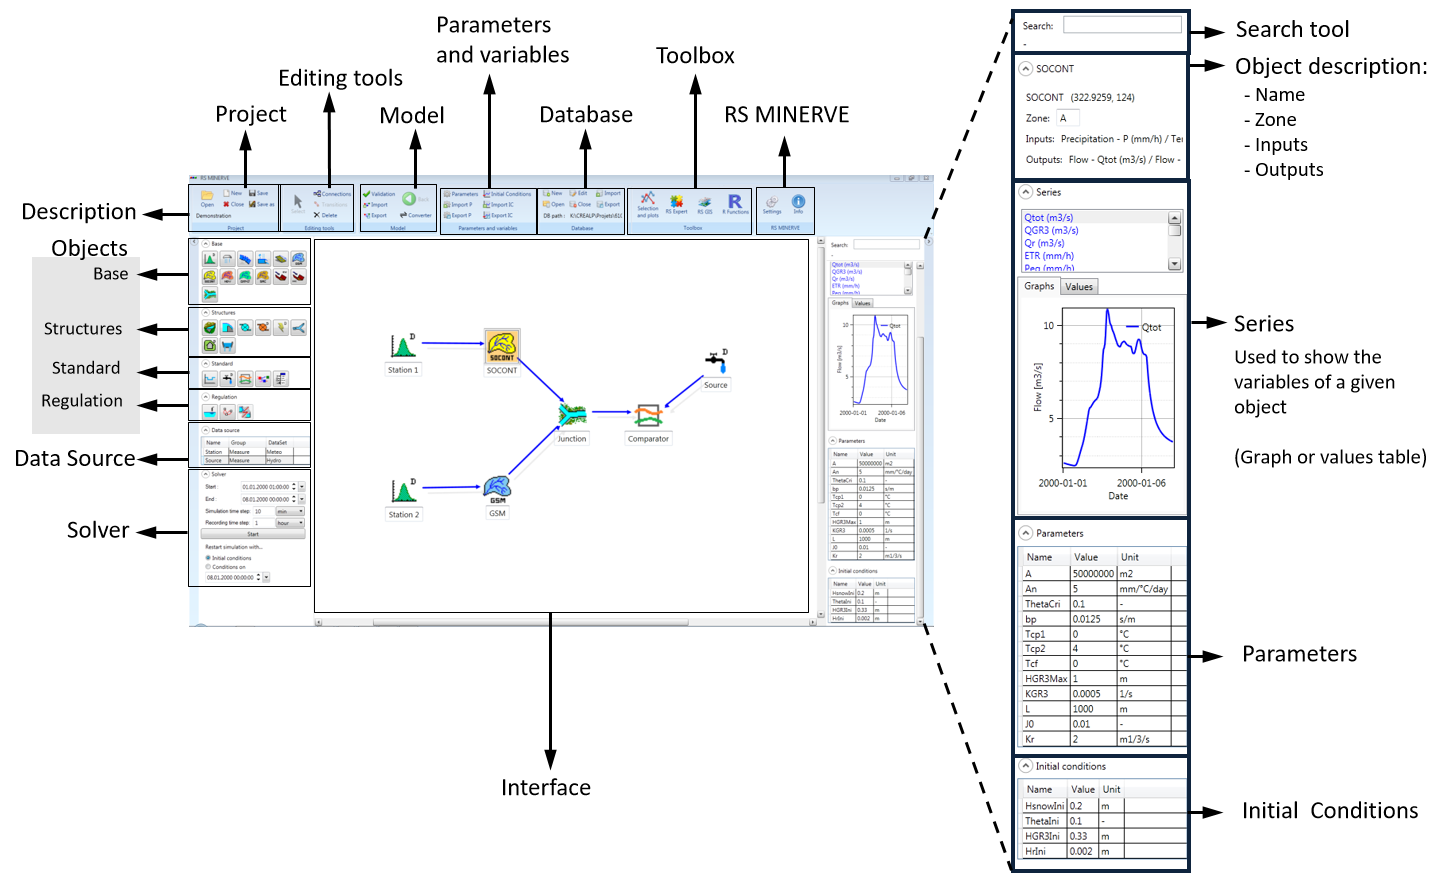
\includegraphics{./figures/fig-rsm_interface.png}

}

\caption{\label{fig-rsm_interface}Structure of the RS MINERVE main
interface}

\end{figure}

\hypertarget{updates}{%
\chapter{Updates}\label{updates}}

When RS MINERVE is opened and if an Internet connection is available, RS
MINERVE connects to the server to check if a new version is available.
If this is the case, the user is invited to install the new version by
accepting the update.

\begin{figure}

{\centering 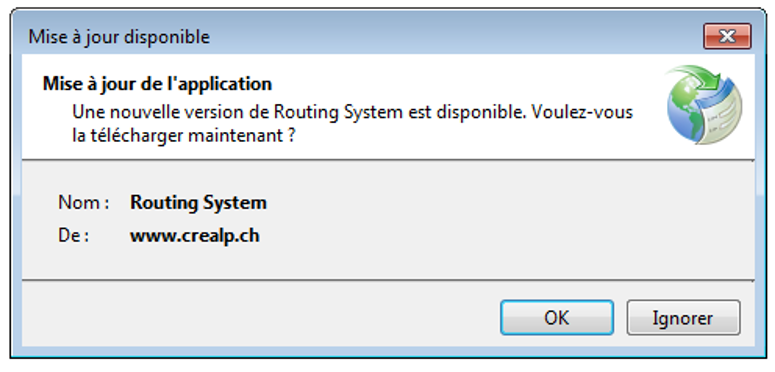
\includegraphics{./figures/fig-installation_updates.png}

}

\caption{\label{fig-installation_updates}Installation of updates}

\end{figure}

\hypertarget{uninstallation-procedure}{%
\chapter{Uninstallation procedure}\label{uninstallation-procedure}}

To uninstall RS MINERVE, use the conventional uninstallation procedure
in Windows.

\hypertarget{the-model-interface}{%
\chapter{The Model interface}\label{the-model-interface}}

The structure of the RS MINERVE main window and the different frames
composing it are presented in Figure~\ref{fig-rsm_interface}.

The \emph{Interface} frame (Figure~\ref{fig-rsm_interface}) in the
middle of the RS MINERVE interface allows the visualization of the model
network.

Interaction within the \emph{Interface} is possible with the mouse.

\begin{itemize}
\item
  Use the scroll wheel to zoom in / zoom out
\item
  Press the scroll wheel and move the mouse to move the interface window
\item
  Left click on an object (Figure~\ref{fig-selected_object} (b))
  \(\rightarrow\) Select the object and move it in the interface
\item
  Double-click on an object (the object is highlighted,
  Figure~\ref{fig-selected_object} (c)) \(\rightarrow\) Display the
  \emph{Object description, Series} and other corresponding frames (in
  the right part).
\end{itemize}

\begin{figure}

{\centering 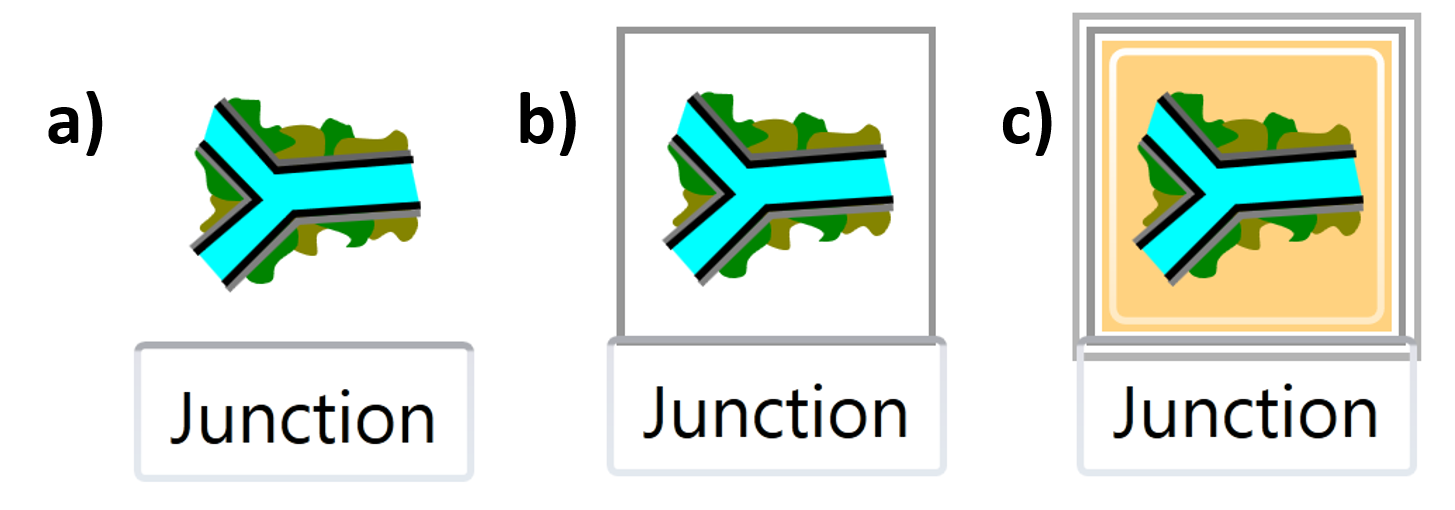
\includegraphics{./figures/fig-selected_object.png}

}

\caption{\label{fig-selected_object}Example of an unselected object (a),
after a left click (b) and after a double-click (c)}

\end{figure}

\hypertarget{the-search-tool}{%
\chapter{The Search tool}\label{the-search-tool}}

To facilitate navigation in the main window, the \emph{Search} tool
(right-frame) allows the user to enter the name of an object. All
corresponding names are listed and a click on the correct one opens the
parent model and highlights the corresponding object.

\begin{figure}

{\centering 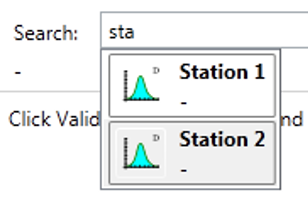
\includegraphics{./figures/fig-search_tool.png}

}

\caption{\label{fig-search_tool}The Search tool}

\end{figure}

\hypertarget{sec-user_intro_settings}{%
\chapter{Settings}\label{sec-user_intro_settings}}

The user can access the settings in the RS MINERVE frame
(Figure~\ref{fig-settings_tab}) and can change the following values:

\begin{itemize}
\item
  The units of inputs, parameters and state variables of RS MINERVE
  (Precipitation, Temperature, Length, Height,\ldots)
\item
  The interpolation method for meteorological values:

  \begin{itemize}
  \item
    Thiessen polygons: for using the nearest meteorological station
  \item
    Shepard method: for values depending on inverse distance weighting
  \end{itemize}
\item
  The Potential Evapotranspiration (ETP) method used in the hydrological
  model. The ETP can be directly taken from Database, or computed with
  one of the following methods:

  \begin{itemize}
  \item
    Turc
  \item
    McGuinness
  \item
    Oudin
  \item
    Uniform ETP
  \end{itemize}
\end{itemize}

Any change is directly applied to the current model. In addition, the
user can also save the current settings as default settings for new
models.

\begin{figure}

{\centering 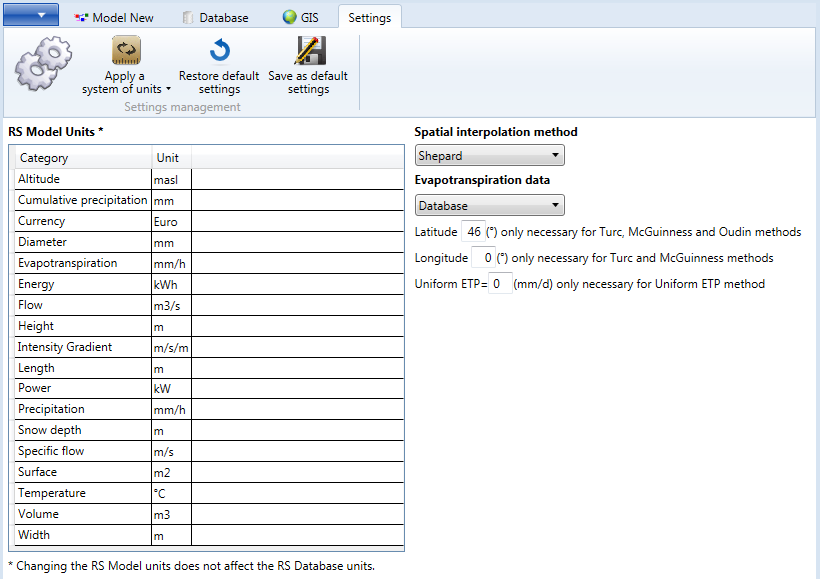
\includegraphics{./figures/fig-settings_tab.png}

}

\caption{\label{fig-settings_tab}RS MINERVE Settings tab}

\end{figure}

\hypertarget{list-of-keyboard-shortcuts-and-mouse-actions}{%
\chapter{List of keyboard shortcuts and mouse
actions}\label{list-of-keyboard-shortcuts-and-mouse-actions}}

The user can use a list of keyboard shortcuts
(Table~\ref{tbl-list_keyboard_shortcuts}) as well as a list of mouse
actions over the graphics (Table~\ref{tbl-list_mouse_actions_graphics}).

\hypertarget{tbl-list_keyboard_shortcuts}{}
\begin{longtable}[]{@{}
  >{\raggedright\arraybackslash}p{(\columnwidth - 2\tabcolsep) * \real{0.2294}}
  >{\raggedright\arraybackslash}p{(\columnwidth - 2\tabcolsep) * \real{0.7706}}@{}}
\caption{\label{tbl-list_keyboard_shortcuts}List of keyboard
shortcuts}\tabularnewline
\toprule()
\endhead
\textbf{Ctrl + N} & New Project \\
\textbf{Ctrl + O} & Open Project \\
\textbf{Ctrl + S} & Save Project \\
\textbf{Ctrl + Shift + S} & Save as Project \\
\textbf{Ctrl + W} & Close Project \\
\textbf{F5} & Start Simulation \\
\textbf{Shift + F5} & Stop Simulation \\
\textbf{Esc} & Back (go to hierarchical higher level), Cancel object
selection (when object type selected in Objects frame) \\
\textbf{Space} & Switch between \emph{Select} and \emph{Connections} \\
\textbf{Ctrl + Space} & Switch between \emph{Select} and
\emph{Transitions} (in a Regulation object only) \\
\textbf{Ctrl} & To select more than one object or series \\
\bottomrule()
\end{longtable}

\begin{longtable}[]{@{}
  >{\raggedright\arraybackslash}p{(\columnwidth - 2\tabcolsep) * \real{0.4700}}
  >{\raggedright\arraybackslash}p{(\columnwidth - 2\tabcolsep) * \real{0.5300}}@{}}
\toprule()
\endhead
\textbf{\emph{OVER THE AXES}} & \\
\textbf{Left click} & - \\
\textbf{Right click and move the mouse} & Displace the current view \\
\textbf{Move the scroll wheel} & Zoom in / zoom out \\
\textbf{Click on scroll wheel and movethe mouse} & Select the zoom
zone \\
\textbf{Double click on scroll wheel} & Back to default zoom \\
\bottomrule()
\end{longtable}

\hypertarget{tbl-list_mouse_actions_graphics}{}
\begin{longtable}[]{@{}
  >{\raggedright\arraybackslash}p{(\columnwidth - 2\tabcolsep) * \real{0.4700}}
  >{\raggedright\arraybackslash}p{(\columnwidth - 2\tabcolsep) * \real{0.5300}}@{}}
\caption{\label{tbl-list_mouse_actions_graphics}List of mouse actions in
graphics}\tabularnewline
\toprule()
\endhead
\textbf{\emph{OVER THE TIME SERIES PLOT}} & \\
\textbf{Left click} & Date and value of the nearest series point \\
\textbf{Right click and move the mouse} & Displace the current view \\
\textbf{Move the scroll wheel} & Zoom in / zoom out \\
\textbf{Click on scroll wheel and move the mouse} & Select the zoom
zone \\
\textbf{Double click on scroll wheel} & Back to default zoom \\
\bottomrule()
\end{longtable}

\hypertarget{references-1}{%
\chapter*{References}\label{references-1}}
\addcontentsline{toc}{chapter}{References}

Rainfall-runoff modelling

RS MINERVE is an object-oriented modeling software. The different
processes are modeled with equation-based objects, presented hereafter
in Section~\ref{sec-user_rainfall_runoff_hydrology} (\emph{Hydrology})
and Section~\ref{sec-user_rainfall_runoff_standard} (\emph{Standard
objects}). \emph{Hydraulic infrastructures} and \emph{Regulation}
objects are presented in
\textbf{?@sec-user\_hydraulic\_infrastructures}.

The implemented hydrological models (Snow-SD, SWMM and GSM-SOCONT) have
been developed within the framework of different research projects,
namely CRUEX (\protect\hyperlink{ref-berod_contribution_1994}{Bérod
1994}), SWURVE
(\protect\hyperlink{ref-schaefli_conceptual_2005}{Schaefli et al. 2005})
and MINERVE\footnote{MINERVE: Modélisation des Intempéries de Nature
  Extrême du Rhône Valaisan et de leurs Effets (Modeling of Rhone
  extreme floods in Valais and their consequences).}
(\protect\hyperlink{ref-hamdi_projet_2003}{Y. Hamdi, Hingray, and Musy
2003}; \protect\hyperlink{ref-hamdi_modeprevision_2005}{Y. Hamdi,
Hingray, and Musy 2005}).

The hydrological models HBV
(\protect\hyperlink{ref-bergstrom_development_1976}{Bergström 1976},
\protect\hyperlink{ref-bergstrom_hbv_1992}{1992}), GR4J
(\protect\hyperlink{ref-perrin_improvement_2003}{Perrin, Michel, and
Andréassian 2003}), SAC (\protect\hyperlink{ref-burnash_nws_1995}{R. J.
C. Burnash 1995}) and SCS
(\protect\hyperlink{ref-mcguinness_comparison_1972}{McGuinness and
Bordne 1972}) are also included in the software RS MINERVE for extending
the hydrological modeling possibilities.

\hypertarget{sec-user_rainfall_runoff_hydrology}{%
\chapter{Hydrology}\label{sec-user_rainfall_runoff_hydrology}}

The \emph{Base objects} are mostly composed of the hydro-meteorological
objects. For more details, see the Technical Manual.

\begin{longtable}[]{@{}
  >{\raggedright\arraybackslash}p{(\columnwidth - 2\tabcolsep) * \real{0.3768}}
  >{\raggedright\arraybackslash}p{(\columnwidth - 2\tabcolsep) * \real{0.6232}}@{}}
\toprule()
\endhead
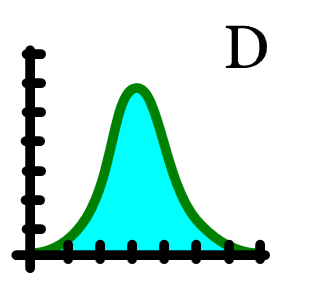
\includegraphics[width=0.44in,height=0.44in]{./figures/fig-icon_object_station.png}
& \textbf{Virtual weather station} - It calculates the local
meteorological conditions (precipitation (P), temperature (T) and
potential evapotranspiration (ETP)) based on observed or forecasted data
from the database and based on Thiessen or Shepard interpolations. In
addition, the ETP can be also calculated either with a constant value or
from one of the different equations proposed by Turc
(\protect\hyperlink{ref-turc_bilan_1955}{1955},
\protect\hyperlink{ref-turc_evaluation_1961}{1961}), McGuinness and
Bordne (\protect\hyperlink{ref-mcguinness_comparison_1972}{1972}) or
Oudin (\protect\hyperlink{ref-oudin_recherche_2004}{2004}). The method
can be selected in the Settings (see
Section~\ref{sec-user_intro_settings}). For more details, please refer
to the Technical Manual of RS MINERVE. \\
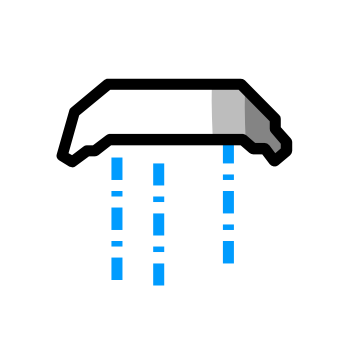
\includegraphics[width=0.44in,height=0.44in]{./figures/fig-icon_object_snow.png}
& \textbf{Snow-SD} - Simulates the time evolution of the snow pack based
on temperature (T) and precipitation (P). The output is an equivalent
precipitation (P\textsubscript{eq}) and the snow height (H) proposed as
input to other models such as \emph{SAC-SMA} or \emph{GR4J}. \\
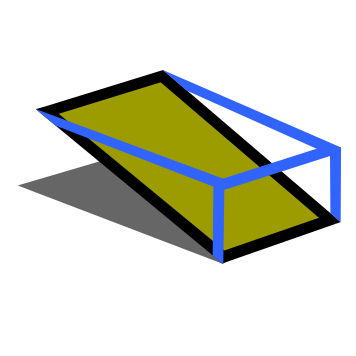
\includegraphics[width=0.44in,height=0.44in]{./figures/fig-icon_object_swmm.png}
& \textbf{Runoff (SWMM)} - The runoff-based hydrograph is calculated
with this object from a net rainfall (i\textsubscript{Net}). \\

\includegraphics[width=0.44in,height=0.44in]{./figures/fig-icon_object_gsm.png}
& \textbf{GSM (Glacial Snow Melt)} - The GSM object combines Snow and
Glacier models. \\

\includegraphics[width=0.44in,height=0.44in]{./figures/fig-icon_object_socont.png}
& \textbf{SOCONT (SOil CONTribution)} - The SOCONT object combines the
Snow, Infiltration (GR3) and Runoff (SWMM) models. \\

\includegraphics[width=0.44in,height=0.44in]{./figures/fig-icon_object_hbv.png}
& \textbf{HBV} - This integrated rainfall-runoff model is based on the
HBV model. Using a precipitation (P), a temperature (T) and a potential
evapotranspiration (ETP) as inputs, it produces a total discharge
(Q\textsubscript{tot}) composed of a run-off flow (Q\textsubscript{r}),
an interflow (Q\textsubscript{u}) and a baseflow
(Q\textsubscript{l}). \\

\includegraphics[width=0.44in,height=0.44in]{./figures/fig-icon_object_gr4j.png}
& \textbf{GR4J} - This object is based on the GR4J model, containing 4
parameters. Using an equivalent precipitation (P\textsubscript{eq}) and
a potential evapotransipration (ETP) as inputs, an outflow is
calculated. \\

\includegraphics[width=0.44in,height=0.44in]{./figures/fig-icon_object_sac.png}
& \textbf{SAC} - The SAC-SMA (Sacramento-Soil Moisture Account) object
uses an equivalent precipitation (P\textsubscript{eq}) and a potential
evapotranspiration (ETP) as inputs and provides an outflow at the outlet
of the sub-basin. \\

\includegraphics[width=0.44in,height=0.44in]{./figures/fig-icon_object_scs.png}
& \textbf{SCS} - The SCS (Soil Conservation Service) object focuses on
specific events modelling mainly for small watersheds. It is a
simplified procedure for assessing an event hydrograph using limited
input data (precipitation). \\
\bottomrule()
\end{longtable}

\hypertarget{sec-user_rainfall_runoff_rivers}{%
\chapter{Rivers}\label{sec-user_rainfall_runoff_rivers}}

Different \emph{Rivers objects} are proposed by RS MINERVE:

\begin{longtable}[]{@{}
  >{\raggedright\arraybackslash}p{(\columnwidth - 2\tabcolsep) * \real{0.3662}}
  >{\raggedright\arraybackslash}p{(\columnwidth - 2\tabcolsep) * \real{0.6338}}@{}}
\toprule()
\endhead
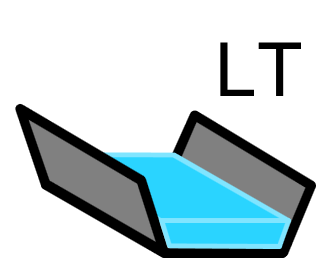
\includegraphics[width=0.44in,height=0.44in]{./figures/fig-icon_object_lagtime.png}
& \textbf{Lag-Time} - The Lag-Time river calculates a river transition
based on a lag-time but does not produce any attenuation of the flow. \\

\includegraphics[width=0.44in,height=0.44in]{./figures/fig-icon_object_kinem.png}
& \textbf{Kinematic Wave} - The flow is transferred based on the
Kinematic wave equations. \\

\includegraphics[width=0.44in,height=0.44in]{./figures/fig-icon_object_musking.png}
& \textbf{Muskingum-Cunge} - The flow is transferred based on the
Muskingum-Cunge (\protect\hyperlink{ref-cunge_subject_1969}{1969},
\protect\hyperlink{ref-cunge_polycopie_1991}{1991}) equations. \\
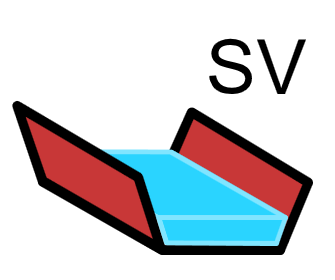
\includegraphics[width=0.44in,height=0.44in]{./figures/fig-icon_object_stvenant.png}
& \textbf{St-Venant} - The flow is transferred based on the St-Venant
equations. \\
\bottomrule()
\end{longtable}

\hypertarget{sec-user_rainfall_runoff_standard}{%
\chapter{Standard}\label{sec-user_rainfall_runoff_standard}}

The \emph{Standard objects} are complementary but generally necessary
for feeding, structuring and calibrating the model.

\begin{longtable}[]{@{}
  >{\raggedright\arraybackslash}p{(\columnwidth - 2\tabcolsep) * \real{0.3959}}
  >{\raggedright\arraybackslash}p{(\columnwidth - 2\tabcolsep) * \real{0.6041}}@{}}
\toprule()
\endhead

\includegraphics[width=0.44in,height=0.44in]{./figures/fig-icon_object_junction.png}
& \textbf{Junction} - This object allows calculating the addition of
different flow inputs (also coming from hydraulic infrastructures). \\
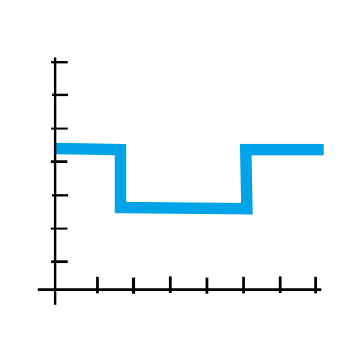
\includegraphics[width=0.44in,height=0.44in]{./figures/fig-icon_object_timeseries.png}
& \textbf{Time series} - Data can be provided to the model as time
series (time in seconds). Data of any type (Flow, Temperature,
Precipitation, ETP,...) can be directly transferred to other objects. \\
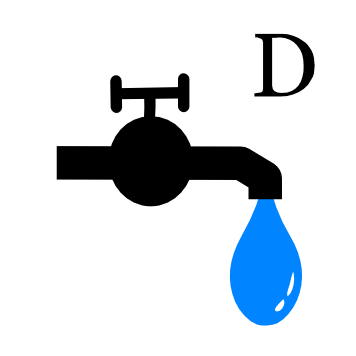
\includegraphics[width=0.44in,height=0.44in]{./figures/fig-icon_object_source.png}
& \textbf{Source} - Data can be also loaded from a database.
\emph{Sources} are mostly used to define flow time series for turbine or
pump flow and as reference flow for calibration (with a
\emph{Comparator} object). \\

\includegraphics[width=0.44in,height=0.44in]{./figures/fig-icon_object_comparator.png}
& \textbf{Comparator} - This object is used to compare the results of a
simulation with a reference data coming from another object, generally a
\emph{Source}. Both objects are connected to the \emph{Comparator} for
results comparison. \\
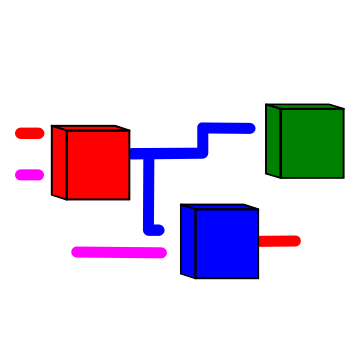
\includegraphics[width=0.44in,height=0.44in]{./figures/fig-icon_object_submodel.png}
& \textbf{Submodel} - A combination of objects can be saved as a
submodel and integrated as such in a model. \\
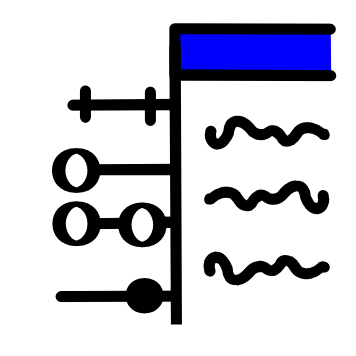
\includegraphics[width=0.44in,height=0.44in]{./figures/fig-icon_object_group_inter.png}
& \textbf{Group Interface} - It allows transferring the input or output
variables between different hierarchical levels. \\
\bottomrule()
\end{longtable}

For hydraulic infrastructures objects and regulation objects, please
refer to \textbf{?@sec-user\_hydraulic\_infrastructures}.

\hypertarget{sec-user_rainfall_runoff_creation_model}{%
\chapter{Creation of a hydrological
model}\label{sec-user_rainfall_runoff_creation_model}}

The steps to create a hydrological model for a natural basin (without
hydraulic infrastructures) are presented in this chapter.

To create the model

\begin{itemize}
\item
  {Open RS MINERVE.}
\item
  {Click on the type of object to be added (\emph{Objects} frame,
  Figure~\ref{fig-rsm_interface}). With the pencil, click in the
  \emph{Interface} to add the object. Repeat the operation for all
  objects. If the wrong object is selected in the \emph{Objects} frame,
  use the \emph{Esc} key to cancel.}
\item
  {Select \emph{Connections} in the \emph{Editing tools} frame
  (Figure~\ref{fig-rsm_interface}) or press the s\emph{pace} key to
  switch, interconnect the objects with blue arrows in the sense of flow
  and select the variables(s) concerned by the connections in the
  pop-ups (Figure~\ref{fig-simple_model_example}).\footnote{In the
    absence of water flow, connect arrows in the sense of information
    transfer.}}
\item
  {Choose \emph{Select} in the \emph{Editing tools} frame or press the
  \emph{space} key to switch.}
\item
  {By clicking on each object separately,}

  \begin{itemize}
  \item
    {Rename the objects.}
  \item
    {Modify their fixed parameters (such as coordinates for the Station
    and surface for main hydrological objects) in the \emph{Parameters}
    frame (Figure~\ref{fig-rsm_interface}). See Appendix 1 for a
    complete list of parameters and initial conditions.}
  \item
    {Define the \emph{Zone} of each object in the \emph{Object} frame
    (Figure~\ref{fig-rsm_interface})\footnote{The concept of
      \emph{Zones} allows the modification of a parameter or initial
      condition to all the objects contained in the selected zone(s) by
      attributing a unique value.}} {Use ``Tab'' to validate the
    \emph{Zone} number.}
  \end{itemize}
\end{itemize}

\begin{figure}

{\centering 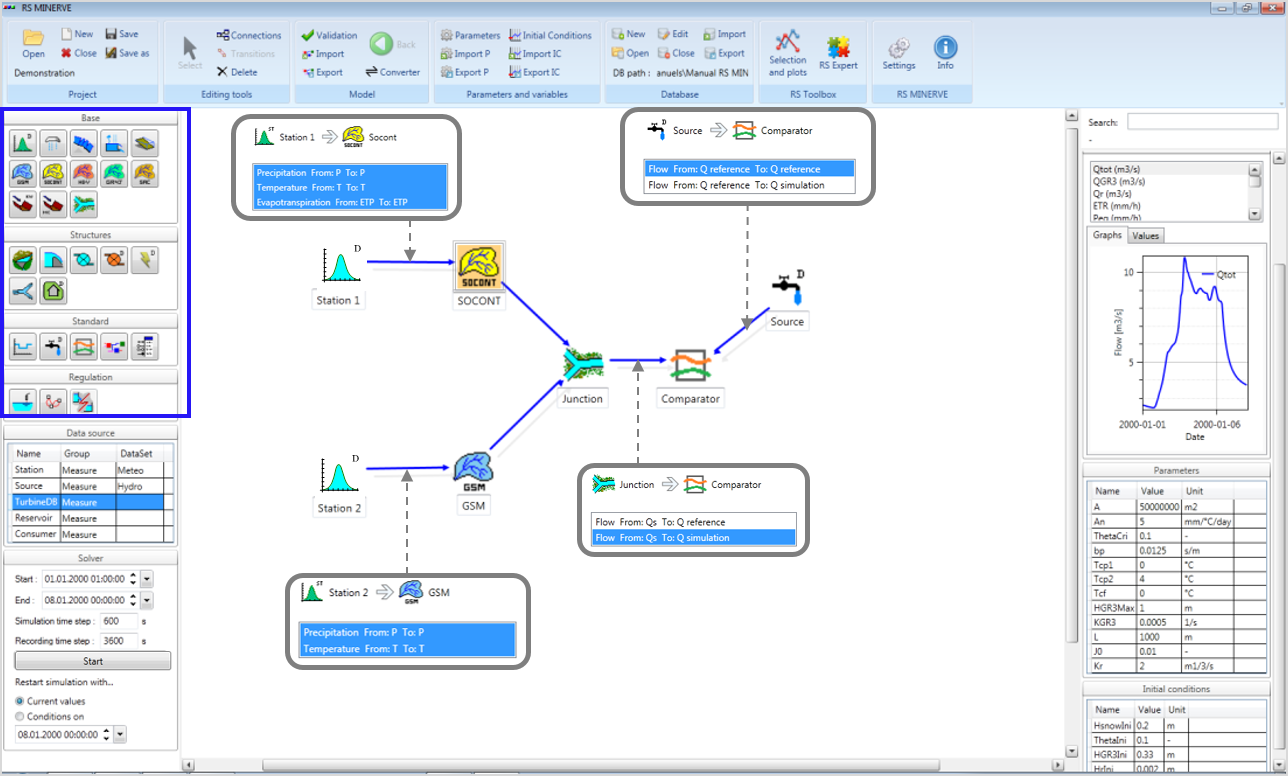
\includegraphics{./figures/fig-simple_model_example.png}

}

\caption{\label{fig-simple_model_example}Example of a simple model}

\end{figure}

To define the \emph{Parameters} of the model objects:

\begin{itemize}
\item
  {Click on
  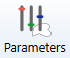
\includegraphics[width=0.2in,height=0.2in]{./figures/fig-parameters_button.png}
  \emph{Parameters} in the \emph{Parameters and Variables} frame
  (Figure~\ref{fig-rsm_interface}).}
\item
  {Select an \emph{Object type} and a \emph{Zone Id} in the
  \emph{Selection} frame (Figure~\ref{fig-selection_frame}). Use
  \emph{Ctrl} to select more than one Zone ID.}
\item
  In the \emph{Parameters management} frame
  (fig-param\_management\_frame, left), the parameters of the selected
  object type are listed. Parameters with identical value in all objects
  of the selected zone(s) are checked by default. The objects contained
  in the zone(s) and their respective parameter values are displayed in
  the \emph{Objects list} (fig-param\_management\_frame, right).
\item
  {Define the parameters to be calibrated, i.e.~uniformly modified, by
  checking and unchecking the parameters in the \emph{Parameters
  management} frame (the {[}x{]} column, fig-param\_management\_frame,
  left).}
\item
  {Modify in the \emph{Parameters management} frame the values of the
  \emph{Parameters} to be calibrated and click on \emph{Apply selected
  changes}. (Alternatively, individually modify the values of each
  object in the \emph{Objects} list (fig-param\_management\_frame,
  right)).}
\item
  {Repeat the procedure for all object types in each zone.}
\end{itemize}

\begin{figure}

{\centering 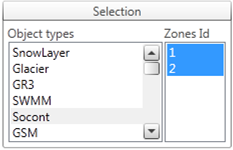
\includegraphics{./figures/fig-selection_frame.png}

}

\caption{\label{fig-selection_frame}Selection frame}

\end{figure}

\begin{figure}

{\centering 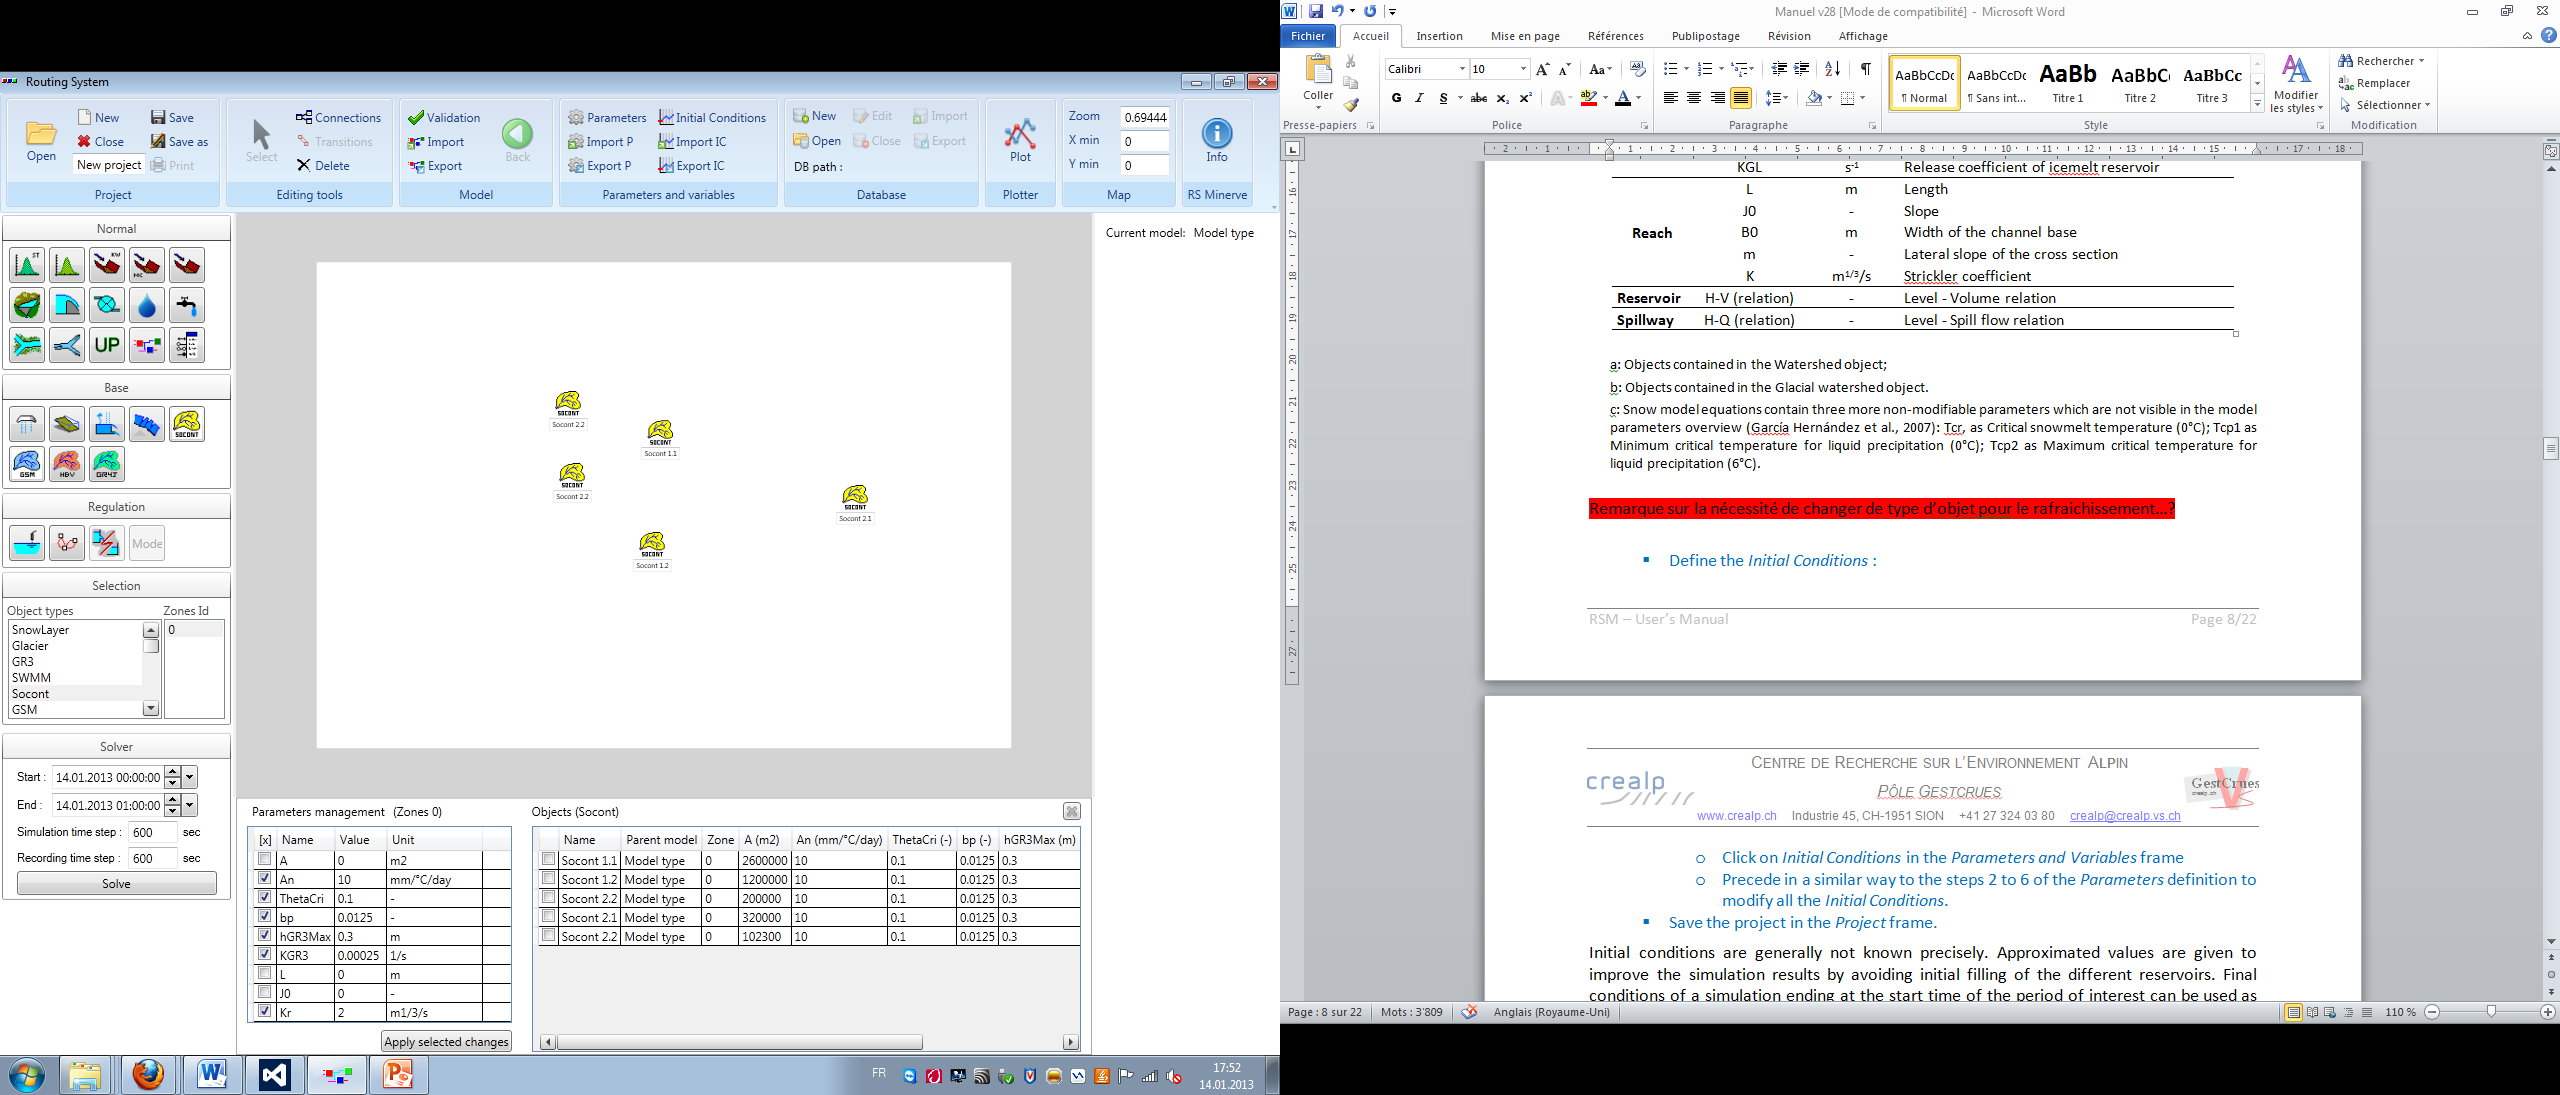
\includegraphics{./figures/fig-param_management_frame.png}

}

\caption{\label{fig-param_management_frame}Left: Parameters management
frame; Right: Objects of the selected zone(s) and their parameters}

\end{figure}

To define the \emph{Initial Conditions}:

\begin{itemize}
\item
  {Click on \emph{Initial Conditions} in the \emph{Parameters and
  Variables} frame (Figure~\ref{fig-rsm_interface}).}
\item
  {Proceed in a similar way than for the \emph{Parameters} definition to
  modify all the \emph{Initial Conditions}.}
\end{itemize}

Initial conditions are generally not known precisely. Approximated
values can be entered to improve the simulation results. Final
conditions of a previous simulation ending at the start time of the
period of interest can be used as current initial conditions to improve
the results.

To save the project:

\begin{itemize}
\item
  {Click on \emph{Save} in the \emph{Project} frame
  (Figure~\ref{fig-rsm_interface}).}
\item
  {Define the file name and save.}
\end{itemize}

\hypertarget{sec-user_rainfall_runoff_export_submodel}{%
\chapter{Exportation of a
submodel}\label{sec-user_rainfall_runoff_export_submodel}}

Combinations of objects can be exported and later imported as
\emph{Submodel} objects in a complete model. This allows the
structuration of the model by organizing it in different hierarchical
levels.

\begin{itemize}
\item
  {Add a
  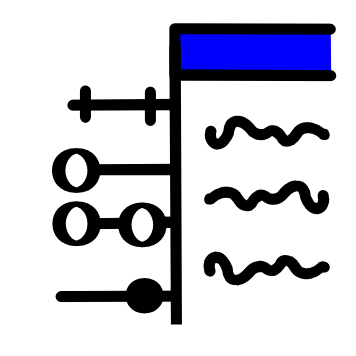
\includegraphics[width=0.2in,height=0.2in]{./figures/fig-icon_object_group_inter.png}\emph{Group
  Interface} to the combination of objects to be exported.\footnote{Group
    Interfaces are required to assemble a submodel with the upper
    hierarchical level. It allows transferring the input and/or output
    variables.}}
\item
  {Link the output object of the model (\emph{Junction} in
  Figure~\ref{fig-addition_group_interface}) to the \emph{Group
  Interface}. Select the link(s) to be created in the pop-up
  (\emph{Flow} in the example of
  Figure~\ref{fig-addition_group_interface}).\footnote{If only one link
    can be created, it is selected by default. If more than one link is
    possible, none is selected.}}
\item
  {Export the active model with the
  
\includegraphics[width=0.17in,height=0.17in]{./figures/fig-icon_export_model.png}
  \emph{Export} button in the \emph{Model} frame
  (Figure~\ref{fig-rsm_interface}).\footnote{During the exportation,
    only the elements contained in the active hierarchical level,
    including all the submodels and objects, are considered.
    Hierarchically higher elements are not exported.}}
\item
  {Create a new project with the \emph{New} button in the \emph{Project}
  frame.\footnote{Or, alternatively, open a project with Project
    \(\rightarrow\) Open.}}
\item
  {Import the \emph{Submodel} with the
  
\includegraphics[width=0.17in,height=0.17in]{./figures/fig-icon_import_model.png}
  \emph{Import} button in the \emph{Model} frame.}
\item
  {Open the
  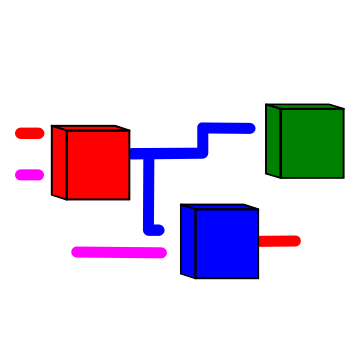
\includegraphics[width=0.16in,height=0.16in]{./figures/fig-icon_object_submodel.png}
  \emph{Submodel} with a right-click on it. The model previously created
  appears.}
\item
  {Return to the upper hierarchical level with the
  
\includegraphics[width=0.15in,height=0.15in]{./figures/fig-icon_back_button.png}
  \emph{Back} button (\emph{Model} frame) or by pressing the \emph{Esc}
  button.}
\item
  {Add a \emph{Junction} object and link the \emph{Submodel} to the new
  \emph{Junction} (Figure~\ref{fig-link_submodel_junction}). In the
  example of Figure~\ref{fig-link_submodel_junction}, the flow of the
  new \emph{Junction} now corresponds to the flow of the \emph{Junction}
  in the \emph{Submodel}.}
\end{itemize}

\begin{figure}

{\centering 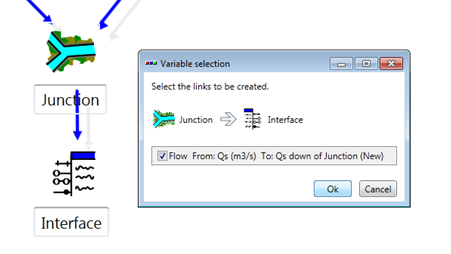
\includegraphics{./figures/fig-addition_group_interface.png}

}

\caption{\label{fig-addition_group_interface}Addition of a \emph{Group
Interface} to the combination of objects to be exported as submodel}

\end{figure}

\begin{figure}

{\centering 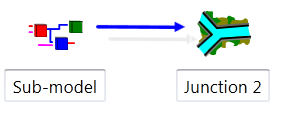
\includegraphics{./figures/fig-link_submodel_junction.png}

}

\caption{\label{fig-link_submodel_junction}Link the \emph{Submodel} to a
\emph{Junction}}

\end{figure}

At the same time, if a \emph{Submodel} receives also an input from
upstream, a second \emph{Group Interface} has to be added in the
\emph{Submodel} and linked to the object receiving the incoming
variables. \emph{Group Interfaces} can support more than one variable as
input and/or as output.

Submodels can also be created by adding an empty
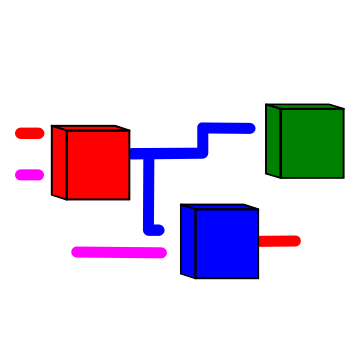
\includegraphics[width=0.2in,height=0.2in]{./figures/fig-icon_object_submodel.png}
\emph{Submodel} object\footnote{By selecting \emph{Submodel} in the
  Standard objects frame and adding the object in the \emph{Interface}.}
and then adding the adequate objects in the \emph{Submodel} (opened with
a right-click). In a similar way, objects can be added to or deleted
from imported \emph{Submodels}.

Modifying the \emph{Zone} of a \emph{Submodel} modifies the zone of all
the objects contained in the \emph{Submodel}.

\hypertarget{sec-user_rainfall_runoff_model_conversion}{%
\chapter{Model
conversion}\label{sec-user_rainfall_runoff_model_conversion}}

The conversion between different hydrological models is possible with
the button ``Converter'' of the Model Properties frame
(Figure~\ref{fig-model_properties_frame}).

\begin{figure}

{\centering 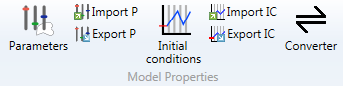
\includegraphics{./figures/fig-model_properties_frame.png}

}

\caption{\label{fig-model_properties_frame}Model properties frame}

\end{figure}

The model conversion is direct for all hydrological model as presented
in Figure~\ref{fig-conversion_between_objects}. For achieving the
conversion, initial and final hydrological model types are selected.
Then, the zone(s) and the object(s) to convert are chosen
(Figure~\ref{fig-example_conversion_hbv_socont}).

In the current version, only the parameter A (Surface) is transferred to
the new model. All other parameters are fixed to the by default values
of each model.

\begin{figure}

{\centering 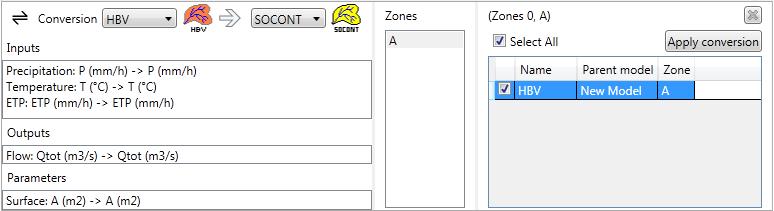
\includegraphics{./figures/fig-example_conversion_hbv_socont.png}

}

\caption{\label{fig-example_conversion_hbv_socont}Example of a
conversion between HBV and SOCONT}

\end{figure}

If the converted model does not need all inputs, a message informs that
one of the inputs is deleted, as presented in
Figure~\ref{fig-example_conversion_hbv_sac} for the input
\emph{Temperature}.

\begin{figure}

{\centering 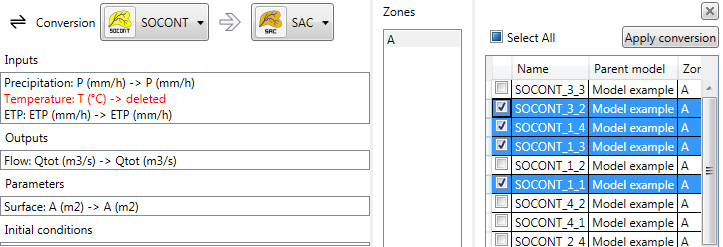
\includegraphics{./figures/fig-example_conversion_hbv_sac.png}

}

\caption{\label{fig-example_conversion_hbv_sac}Example of a conversion
between a model HBV and SAC, where the input Temperature is deleted}

\end{figure}

Finally, if the converted model needs more inputs than the original one,
a message informs that one or several inputs need to be added, as
presented in Figure~\ref{fig-example_conversion_sac_hbv} for the input
\emph{Temperature}. In that case, this/these input(s) is/are added
between the station and the model (If the data comes from several
\emph{Stations} or \emph{Time Series}, the user needs to link himself
and to select the correct inputs among all possibilities).

\begin{figure}

{\centering 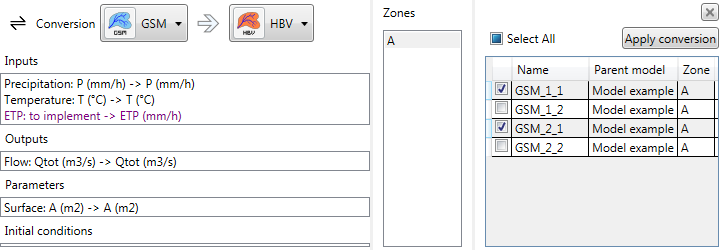
\includegraphics{./figures/fig-example_conversion_sac_hbv.png}

}

\caption{\label{fig-example_conversion_sac_hbv}Example of a conversion
between a model SAC and HBV, where the input Temperature has to be
implemented by the user}

\end{figure}

Regarding the outputs, the total discharge (Qtot or Q depending on the
model) is directly linked to the downstream object after the conversion.

If any other discharge is linked downstream, e.g.~the Qr in the SOCONT
model to a junction, the link is deleted after conversion.

\begin{figure}

{\centering 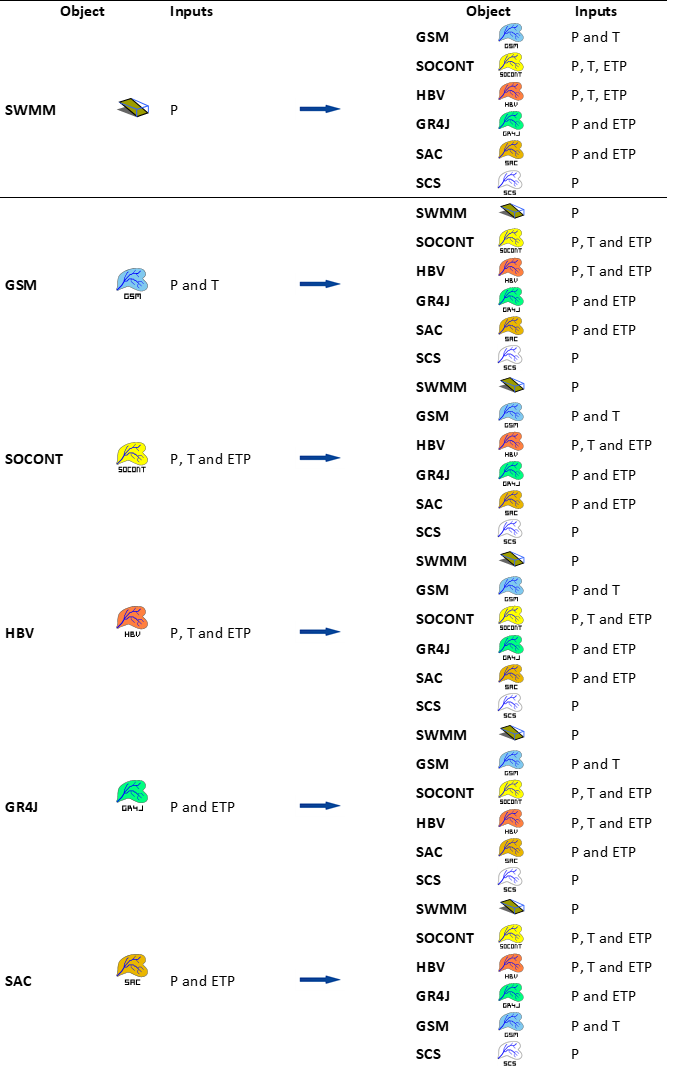
\includegraphics{./figures/fig-conversion_between_objects.png}

}

\caption{\label{fig-conversion_between_objects}Conversions between
objects}

\end{figure}

\hypertarget{sec-user_rainfall_runoff_subbasin_param}{%
\chapter{Single sub-basin
parametrization}\label{sec-user_rainfall_runoff_subbasin_param}}

The parametrization (or calibration) process aims to progressively
improve the model to fit the simulated data to the reference data (e.g.
the observations) by iteratively adjusting the object's parameters.

To proceed to the optimal parametrization (or calibration), observed
data are required as comparison basis for the simulated data. Sites of
measure stations generally define outlets of sub-basins since they
represent the location of comparison (simulated data vs.~observed
data).\footnote{Other factors are also considered during the basin
  division such as reservoir locations or river junctions.}

For simplicity, division into zones generally respects the sub-basin's
division. However, this is not compulsory and a zone can correspond to
several sub-basins or one sub-basin can be divided into several zones.
In this subchapter, it is assumed that the sub-basin is composed of a
single zone.

\hypertarget{sec-user_rainfall_runoff_model_performance}{%
\section{Model's performance
evaluation}\label{sec-user_rainfall_runoff_model_performance}}

Before adjusting the parameters, the current performance of the model is
evaluated.

\begin{itemize}
\item
  {Click on the
  
\includegraphics[width=0.2in,height=0.2in]{./figures/fig-icon_object_comparator.png}
  \emph{Comparator} object which has been added and connected as
  presented in Figure~\ref{fig-simple_model_example}.}
\item
  {In the \emph{Series} frame (Figure~\ref{fig-frames_parametrization}),
  select \emph{Q\textsubscript{reference}} and
  \emph{Q\textsubscript{simulation}} (use \emph{Ctrl} to select both).}
\item
  {Visualize the actual results:}

  \begin{itemize}
  \item
    {In the \emph{Series frame}, both curves are plotted together under
    \emph{Graphs}.}
  \item
    {In the \emph{Comparator} frame, seven performance indicators are
    provided (read the Technical Manual for more information).}

    \begin{itemize}
    \item
      {Nash coefficient}
    \item
      {Nash-ln coefficient}
    \item
      {Pearson Correlation Coefficient}
    \item
      {Kling-Gupta Efficiency}
    \item
      {Bias Score}
    \item
      {Relative Root Mean Square Error}
    \item
      {Relative Volume Bias}
    \item
      {Normalized Peak Error}
    \end{itemize}
  \end{itemize}
\end{itemize}

\hypertarget{sec-user_rainfall_runoff_param_adjustment}{%
\section{Manual parameters
adjustment}\label{sec-user_rainfall_runoff_param_adjustment}}

Based on the current model's performance, object's parameters can be
adjusted to improve the next run's performance.

\begin{itemize}
\item
  {Click on \emph{Parameters} in the \emph{Parameters and variables}
  frame (Figure~\ref{fig-frames_parametrization}).}
\item
  {Select in the \emph{Selection} frame
  (Figure~\ref{fig-frames_parametrization}) the type of object to be
  modified and the corresponding zone.}
\item
  {Modify the selection (checks) of parameters in the \emph{Parameters
  Management} frame to select only the ones to be calibrated (i.e.~to be
  uniformly modified).}
\item
  {Modify the values of the selected parameters and click on \emph{Apply
  selected changes}. Parameters are modified in the listed objects.}
\item
  {Proceed in a similar way for all object types.}
\item
  {Modify also the initial conditions to fit better the reference data.}
\item
  {After running the model, analyze the results in the comparator and
  modify again the parameters when necessary.}
\end{itemize}

\begin{figure}

{\centering 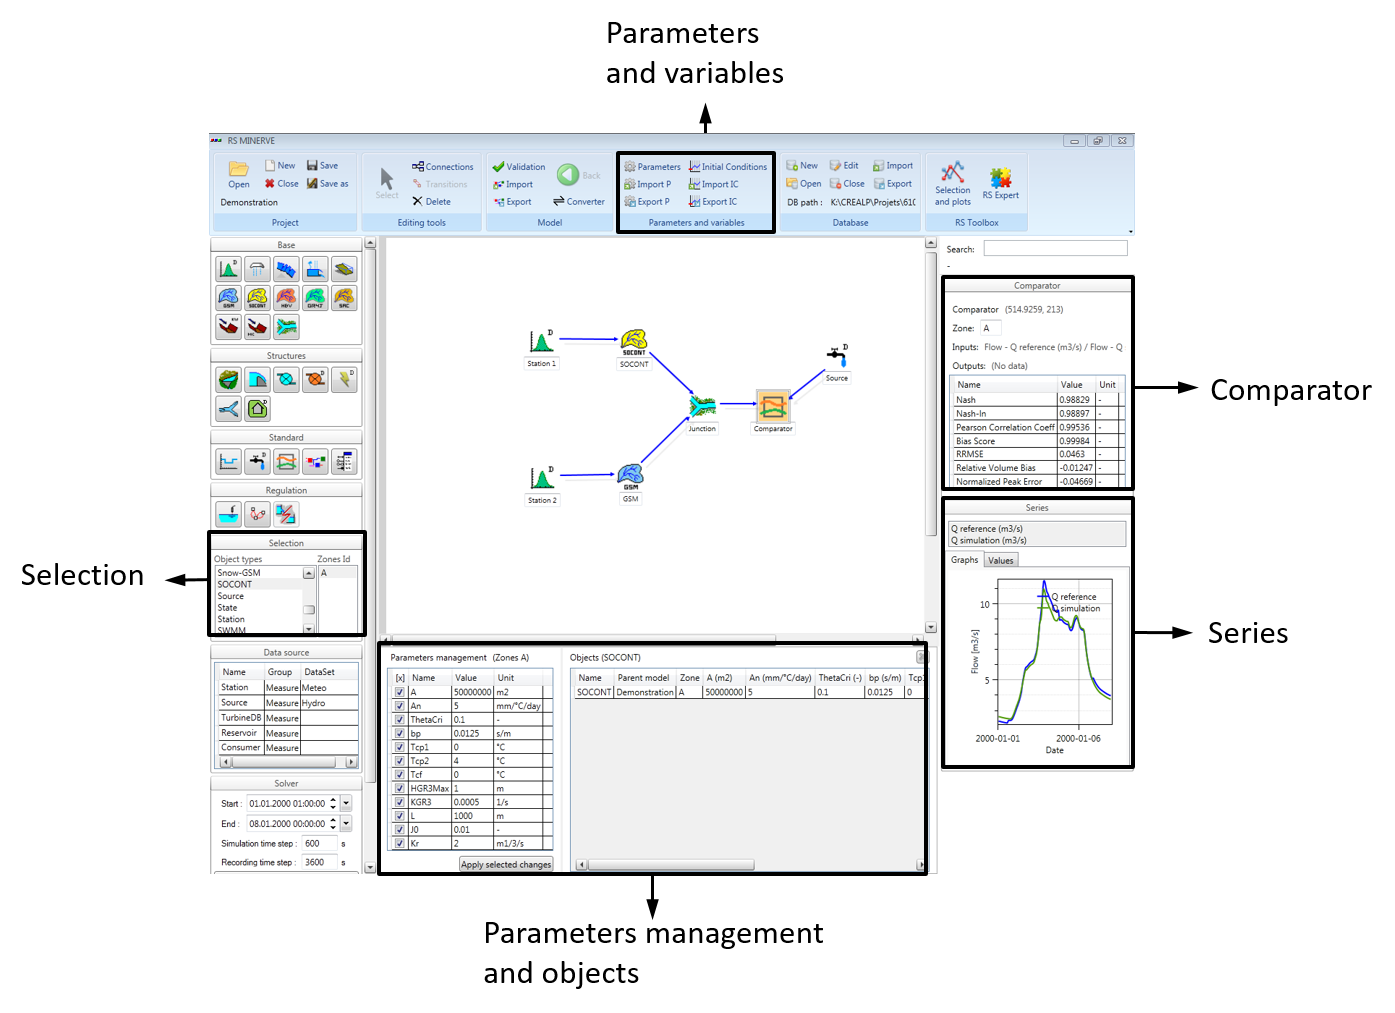
\includegraphics{./figures/fig-frames_parametrization.png}

}

\caption{\label{fig-frames_parametrization}Frames used for the
parametrization}

\end{figure}

The procedure is iterative until the simulation results are considered
sufficiently satisfying for a specified zone.

\emph{Parameters} and \emph{Initial conditions} can be exported to be,
later, imported again. Use \emph{Export P} and \emph{Import P} for the
parameters and \emph{Export IC} and \emph{Import IC} for the initial
conditions in the \emph{Parameters and variables} frame
(Figure~\ref{fig-frames_parametrization}). The parameters or initial
conditions can be saved as .txt file or also as .xlsx file with one
sheet per object type.

\hypertarget{sec-user_rainfall_runoff_auto_param_adjustment}{%
\section{Automatic parameters
adjustment}\label{sec-user_rainfall_runoff_auto_param_adjustment}}

An automatic calibration can be also achieved thanks to a specific tool
developed in the Expert module. Please the
Section~\ref{sec-user_expert_module_calibrator} for more information.

\hypertarget{sec-user_rainfall_runoff_basin_param}{%
\chapter{Complete basin
parametrization}\label{sec-user_rainfall_runoff_basin_param}}

When a basin is composed of many sub-basins, the parametrization has to
be progressively achieved from upstream to downstream in the basin. By
proceeding as such, contributions from the upstream calibrated
sub-basin(s) are considered as input(s) to the downstream sub-basin on
which the parametrization is performed. Parameters are modified for the
concerned sub-basin to obtain the best possible results at the outlet of
the sub-basin. The calibration module
(Section~\ref{sec-user_expert_module_calibrator}) can realize multiple
parametrizations for calibrating these complex basins from upstream to
downstream.

Depending on the quality of the simulation results, inputs from upstream
sub-basins can be replaced in the parametrization process by observed
data at the entrance of the sub-basin being calibrated.

\hypertarget{references-2}{%
\chapter*{References}\label{references-2}}
\addcontentsline{toc}{chapter}{References}

Hydraulic infrastructures modelling

\textbf{?@sec-user\_rainfall\_runoff} presents the different steps to
create a hydrological model without any hydraulic infrastructures.
\textbf{?@sec-user\_hydraulic\_infrastructures} explains how
infrastructures like reservoirs, turbines or spillways are implemented
in RS MINERVE.

Hydraulic infrastructures are listed in
Section~\ref{sec-user_hydraulic_infrastructures_list}, and objects used
for automatic regulation are presented in Chapters
Section~\ref{sec-user_hydraulic_infrastructures_hydropower} and
Section~\ref{sec-user_hydraulic_infrastructures_planner}.

\hypertarget{sec-user_hydraulic_infrastructures_list}{%
\chapter{Infrastructures}\label{sec-user_hydraulic_infrastructures_list}}

\begin{longtable}[]{@{}
  >{\raggedright\arraybackslash}p{(\columnwidth - 2\tabcolsep) * \real{0.2662}}
  >{\raggedright\arraybackslash}p{(\columnwidth - 2\tabcolsep) * \real{0.7338}}@{}}
\toprule()
\endhead

\includegraphics[width=0.44in,height=0.44in]{./figures/fig-icon_object_reservoir.png}
& \textbf{Reservoir} - Water level and volume evolution are simulated
based on a ``Level-Volume'' relation and an initialreservoir level. \\
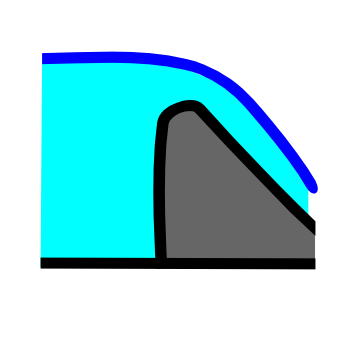
\includegraphics[width=0.44in,height=0.44in]{./figures/fig-icon_object_hq.png}
& \textbf{HQ} - Based on a level-discharge relation, it allows
integration of level-based outflows to reservoirs (such as spillways,
gates, orifices,\ldots). \\
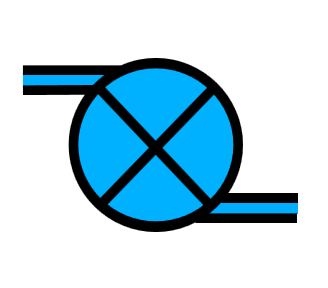
\includegraphics[width=0.44in,height=0.44in]{./figures/fig-icon_object_turbine.png}
& \textbf{Turbine} - It calculates the turbine or pump flow from a
reservoir, based on a \emph{Wanted Discharge} defined in the same object
by a time-discharge series. \\

\includegraphics[width=0.44in,height=0.44in]{./figures/fig-icon_object_turbinedb.png}
& \textbf{TurbineDB} - The TurbineDB object works as the \emph{Turbine}
object but is directly based on data provided by the database. It is
equivalent to the combination of a turbine and a source. \\
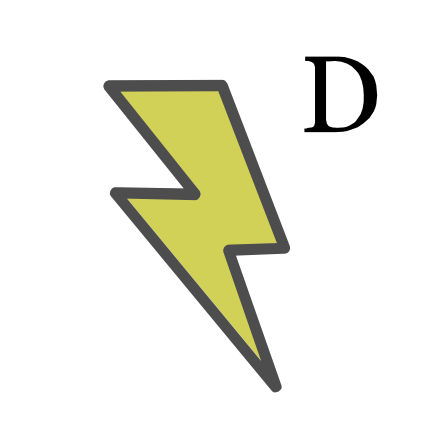
\includegraphics[width=0.44in,height=0.44in]{./figures/fig-icon_object_hydropower.png}
& \textbf{Hydropower} - This object calculates the power and the
revenue, normally produced by a turbine, depending on the discharge and
on the reservoir level. \\
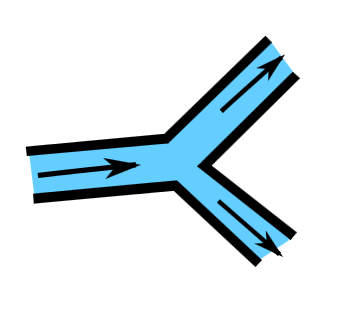
\includegraphics[width=0.44in,height=0.44in]{./figures/fig-icon_object_diversion.png}
& \textbf{Diversion} - This object is used to simulate the separation of
flow based on an ``Inflow - Diverted flow'' relation. It can be used as
a hydrological object but is mostly used as a hydraulic function. \\

\includegraphics[width=0.44in,height=0.44in]{./figures/fig-icon_object_consumer.png}
& \textbf{Consumer} - This object simulates the consumed dischargeof a
user (e.g.: a village or an agricultural field) based on a series from a
database or from a uniform demand. \\
\includegraphics[width=0.44in,height=0.44in]{./figures/fig-icon_object_efficiency.png}
& \textbf{Structure efficiency} - This object computes effects of
discharge losses in a structure like a canal or a pipe based on an
efficiency coefficient. \\
\includegraphics[width=0.44in,height=0.44in]{./figures/fig-icon_object_planner.png}
& \textbf{Planner} - This is a control system consisting of the
definition of a set of management rules, based on conditions. This
object allows you to manage the regulation of reservoirs, turbines,
bottom outlets, etc. \\
\bottomrule()
\end{longtable}

\hypertarget{sec-user_hydraulic_infrastructures_hydropower}{%
\chapter{Addition of a Hydropower
scheme}\label{sec-user_hydraulic_infrastructures_hydropower}}

This chapter presents a general example for the construction of a
hydropower scheme, including a reservoir with a hydropower plant, a
turbine and a spillway.

\hypertarget{addition-of-a-reservoir}{%
\section{Addition of a reservoir}\label{addition-of-a-reservoir}}

To add a reservoir:

\begin{itemize}
\item
  {Select the object \emph{Reservoir} in the Infras\emph{tructures
  objects} frame (2) and add it in the \emph{Interface}.}
\item
  {Link the output of the upstream sub-basin (object \emph{Junction} in
  2) to the \emph{Reservoir}.}
\end{itemize}

\begin{figure}

{\centering \includegraphics{./figures/fig-model_with_reservoir.png}

}

\caption{\label{fig-model_with_reservoir}A regular model with a
reservoir}

\end{figure}

\begin{itemize}
\item
  {Double-click on the \emph{Reservoir} object. The \emph{Reservoir},
  \emph{Series} and \emph{Initial Conditions} frames are opened (2).}
\item
  {In the \emph{Series} frame, select the \emph{H-V} series and open the
  \emph{Values} tab.}
\item
  {By default, the table is empty. Insert the corresponding
  Height-Volume (\emph{H-V}) relation for the reservoir.}
\item
  {Define an initial water elevation (\emph{HIni}) in the \emph{Initial
  conditions} frame.}
\end{itemize}

Alternatively to the last point to define the initial water elevation of
the \emph{Reservoir}, a time series can be saved in the database with a
sensor of Category \emph{Altitude} and Unit \emph{masl}. For each
simulation, RS MINERVE will then search and interpolate the initial
condition from the added time series. To link the \emph{Reservoir} with
the sensor, first select in the \emph{Data Source} frame the
corresponding \emph{Group} and \emph{Dataset}.

Then, in the \emph{Reservoir} frame (right part), click on the
\includegraphics[width=0.15in,height=0in]{./figures/fig-icon_arrow_down_menu.png}
\emph{Select station from Database} button and define the correct
station in the \emph{Station} drop-down list (only stations containing a
sensor with appropriate units are listed). The value in the
\emph{Initial conditions} frame will change after every simulation to
the value interpolated from the time series.

Once a reservoir is implemented, outputs of the reservoir have to be
defined. Water from a reservoir can be exited through different ways. A
combination of \emph{Turbine} (or \emph{TurbineDB}) and
\emph{Hydropower} objects are used to simulate the use of water for
hydropower production. \emph{Regulations} are generally used to
automatize the operation of \emph{Turbine} and \emph{TurbineDB} objects.
Finally, \emph{HQ} objects generate discharges based on
elevation-discharge relations.\footnote{As outputs from the Reservoir
  are defined by downstream objects, output flows (Qs) are considered as
  an \emph{Input} to the \emph{Reservoir} in terms of information flow.
  The corresponding water is thereby withdrawn from the stored volume.
  This implies that at least one output flow has to be defined to
  validate the model.}

All these objects can be used independently and cumulatively. For
example, several turbines can be placed in parallel with one or several
\emph{TurbineDB}(s), \emph{HQ} object(s) and/or \emph{Regulation}(s).
None of them is imperative.

\hypertarget{addition-of-a-turbinedb-object}{%
\section{Addition of a TurbineDB
object}\label{addition-of-a-turbinedb-object}}

The \emph{TurbineDB} object is based on data from a database. Thus,
before adding a \emph{TurbineDB}, data have to be added to the database

\begin{itemize}
\tightlist
\item
  {Open a database (see \textbf{?@sec-user\_database}) and create a
  station with a sensor of category \emph{Flow.} Modify the description
  and insert data for the \emph{TurbineDB} outflow in the \emph{Values}
  tab.}
\end{itemize}

The \emph{TurbineDB} object is then added.

\begin{itemize}
\tightlist
\item
  Select the object \emph{TurbineDB} in the \emph{Structures objects}
  frame

  \begin{enumerate}
  \def\labelenumi{(\arabic{enumi})}
  \tightlist
  \item
    and add it in the \emph{Interface}. Add also a \emph{Junction} to
    which outflow(s) from the \emph{Reservoir} will be linked to.
  \end{enumerate}
\item
  {Switch to \emph{Connections} (\emph{Editing Tools} frame
  \(\rightarrow\) \emph{Connections} or use the \emph{space} key) and
  link the \emph{Reservoir} to the \emph{TurbineDB} object and the
  \emph{TurbineDB} object to the \emph{Junction}
  (Figure~\ref{fig-addition_turbinedb_junction}).}
\end{itemize}

\begin{figure}

{\centering \includegraphics{./figures/fig-addition_turbinedb_junction.png}

}

\caption{\label{fig-addition_turbinedb_junction}Addition of a
\emph{TurbineDB} and a junction}

\end{figure}

\begin{itemize}
\item
  {In the \emph{Data Source} frame (2), select for the line \emph{HPP}
  \footnote{Short for HydroPower Plant, which includes the
    \emph{TurbineDB} and the \emph{Hydropower} objects.} the
  \emph{Group} and \emph{DataSet} corresponding to the sensor created in
  the database.}
\item
  {Double-click on the \emph{TurbineDB} object to open the
  \emph{TurbineDB} frame (right-side). Then, click on the
  \includegraphics[width=0.15in,height=0in]{./figures/fig-icon_arrow_down_menu.png}
  \emph{Select station from Database} button and define the
  corresponding station in the \emph{Station} drop-down list. The link
  between the \emph{TurbineDB} object and the database is now
  operational.}
\item
  {In the \emph{Parameters} frame (Figure~\ref{fig-param_ic_turbine}),
  user can define the reservoir water altitude to start
  (H\textsubscript{on}) or stop (H\textsubscript{off}) the turbine. If
  the value is equal to zero, the turbine operation will be independent
  of the reservoir altitude.}
\item
  {In the \emph{Initial conditions} frame
  (Figure~\ref{fig-param_ic_turbine}), user must define the initial
  turbine status when the water altitude is initially between
  H\textsubscript{on} and H\textsubscript{off}. `Zero' (0) means
  starting the simulation with the turbine OFF and `one' (1) means
  starting with the turbine ON.}
\end{itemize}

Once these parameters specified, the \emph{TurbineDB} object is ready
for use.

\begin{figure}

{\centering \includegraphics{./figures/fig-param_ic_turbine.png}

}

\caption{\label{fig-param_ic_turbine}Parameters and initial conditions
of turbine}

\end{figure}

\begin{figure}

{\centering \includegraphics{./figures/fig-example_turbine_operation.png}

}

\caption{\label{fig-example_turbine_operation}Example of turbine
operation}

\end{figure}

\hypertarget{addition-of-a-hydropower-object}{%
\section{Addition of a Hydropower
object}\label{addition-of-a-hydropower-object}}

The \emph{Hydropower} object calculates the power and the revenue
produced by the discharge of the turbine from the reservoir. The results
depend on the discharge and on the reservoir water level.

\begin{itemize}
\tightlist
\item
  Select the object \emph{Hydropower} in the \emph{Structures objects}
  frame

  \begin{enumerate}
  \def\labelenumi{(\arabic{enumi})}
  \setcounter{enumi}{1}
  \tightlist
  \item
    and add it in the \emph{Interface}
    (Figure~\ref{fig-addition_hydropower}).
  \end{enumerate}
\end{itemize}

\begin{figure}

{\centering \includegraphics{./figures/fig-addition_hydropower.png}

}

\caption{\label{fig-addition_hydropower}Addition of a \emph{Hydropower}
object}

\end{figure}

As the power produced in the hydropower plant depends on the water level
in the reservoir and on the discharge of the turbine, these two
variables (water level and discharge) must be transferred to the
Hydropower object as follows
(Figure~\ref{fig-links_hydropower_reservoir_turbinedb}):

\begin{itemize}
\item
  {Link the \emph{TurbineDB} to the \emph{Hydropower} object so the
  discharge variable can be transferred to the \emph{Hydropower}
  object.}
\item
  {The water level information will be automatically transferred from
  the \emph{Reservoir} to the \emph{Hydropower} object through the
  \emph{TurbineDB} object.}
\end{itemize}

\begin{figure}

{\centering \includegraphics{./figures/fig-links_hydropower_reservoir_turbinedb.png}

}

\caption{\label{fig-links_hydropower_reservoir_turbinedb}Links between
the \emph{Hydropower} object and the \emph{Reservoir} and
\emph{TurbineDB} information}

\end{figure}

\begin{itemize}
\item
  {Double-click on the \emph{Hydropower} object to open its frame
  (right-side). Then, click on the
  \includegraphics[width=0.15in,height=0in]{./figures/fig-icon_arrow_down_menu.png}
  \emph{Select station from Database} button and define the
  corresponding station which contains the \emph{Electricity price}
  series in the \emph{Station} drop-down list. The link between the
  \emph{Hydropower} object and the database is now operational.}
\item
  {In the \emph{Series} frame, select the Q-\(\eta\)
  (discharge-efficiency) series and open the Values tab. Insert data for
  the Q-\(\eta\) relation (manually or copied from a spreadsheet).}
\item
  {In the \emph{Parameters} frame, introduce the features of the
  hydropower plant. In particular the following parameters must be
  specified: the hydropower plant altitude (\(Zcentral\)) in masl; the
  length of the pipe (\(L\)) in m; the diameter of the pipe (\(D\)) in
  m; the Roughness (\(K\)) in m; the kinematic viscosity (\(\nu\)) in
  m\textsuperscript{2}/s; and the default price of electricity, only
  used if no data exists in the database.}
\end{itemize}

The \emph{Hydropower} object is ready for use.

\hypertarget{addition-of-an-hq-object}{%
\section{Addition of an HQ object}\label{addition-of-an-hq-object}}

HQ objects are used to define level-discharge relations to implement
structures such as spillways, orifices or sluice gates. For illustration
purpose, an \emph{HQ} object is used as a spillway in the following
procedure.

\begin{itemize}
\item
  Select the \emph{HQ} object in the \emph{Structures objects} frame (2)
  and add it in the \emph{Interface}.
\item
  Link the \emph{Reservoir} to the \emph{HQ} object and the \emph{HQ}
  object to the \emph{Junction} (Figure~\ref{fig-addition_spillway}).
\end{itemize}

\begin{figure}

{\centering \includegraphics{./figures/fig-addition_spillway.png}

}

\caption{\label{fig-addition_spillway}Addition of a spillway}

\end{figure}

\begin{itemize}
\tightlist
\item
  {Double-click on the \emph{HQ} object. In the \emph{Series} frame,
  select the \emph{H-Q} series and open the \emph{Values} tab. Insert
  data for the \emph{H-Q} relation (manually or copied from a
  spreadsheet).}
\end{itemize}

The \emph{HQ} object is ready for use.

\hypertarget{simulation-with-implemented-structures}{%
\section{Simulation with implemented
structures}\label{simulation-with-implemented-structures}}

Several structures can be added in parallel as illustrated in
Figure~\ref{fig-addition_spillway}. When all objects are created, the
model linked to the database and validated, start the simulation
(Section~\ref{sec-user_hydro_hydrau_simulation_run_model}). Discharges
through the different objects can then be visualized by clicking on each
object (Section~\ref{sec-user_hydro_hydrau_simulation_run_model}) or
within the \emph{Selection and Plots} module
(Section~\ref{sec-user_hydro_hydrau_simulation_selection_plots}).

It is \textbf{important} to remember that discharges generated by
\emph{HQ} objects are defined by the water level in the reservoir. Below
a certain level, no discharge is produced. This is not the case of the
\emph{TurbineDB} objects that withdraws from the reservoir the
discharges defined in the database, without checking if water is
available or not in the reservoir. This might result in a negative
volume in the reservoir (a warning is generated in the \emph{Simulation
report}). In order to generate discharges only when the water is
actually available, \emph{Regulation} objects are necessary.

\hypertarget{sec-user_hydraulic_infrastructures_planner}{%
\chapter{Implementation of a
planner}\label{sec-user_hydraulic_infrastructures_planner}}

The planner object represents a control system that allows the
definition of a set of management rules based on conditions. This object
allows regulating the operation of reservoirs, turbines and hydropower
models in RS MINERVE.

Each rule is defined using one or more conditions (that can be
combined), temporary restrictions (specific dates, hours, days of the
week, or months of the year) and an expected output. The conditions and
the temporary restrictions define the rule to be applied (and
corresponding output). The input values for the conditions can be
defined in different ways: directly taken from the variable of some
object of the full model (e.g., a specific reservoir), its own input or
depending on the state of another rule defined in the same planner. The
output can be generated from a predefined series of values, through the
database, as one of the three possible inputs of the planner object or
by setting a specific value. Furthermore, the output values can be
modified by applying a multiplier and/or additive coefficient(s). A
planner can be connected from all objects and to all objects except to
stations, time series and sources
(Figure~\ref{fig-inputs_outputs_planner}).

Once we have simulated the model, the planner shows at what times each
defined rule has been applied. With all these options, the planner
object is an efficient tool for managing complex systems.

\begin{figure}

{\centering \includegraphics{./figures/fig-inputs_outputs_planner.png}

}

\caption{\label{fig-inputs_outputs_planner}Inputs and outputs for a
\emph{Planner object}}

\end{figure}

\hypertarget{planner}{%
\section{Planner}\label{planner}}

The first part of the Planner window (right frame) shows basic
information about the object
(Figure~\ref{fig-planner_principal_window}).

\begin{figure}

{\centering \includegraphics{./figures/fig-planner_principal_window.png}

}

\caption{\label{fig-planner_principal_window}\emph{Planner} object
principal window}

\end{figure}

To know if the planner is correctly connected in the model, the
exclamation mark should be green; if it is not, the exclamation mark
will be orange and the object will be isolated and not calculated
(Figure~\ref{fig-planner_section}). In that case, it will indicate what
part of the planner element is not correctly defined.

\begin{figure}

{\centering \includegraphics{./figures/fig-planner_section.png}

}

\caption{\label{fig-planner_section}Planner section}

\end{figure}

\begin{itemize}
\tightlist
\item
  {Click on the blue circular arrow (``Clear variable'') to reset inputs
  information after connections are removed.}
\end{itemize}

Figure~\ref{fig-planner_section_example} shows an example with one Input
(Altitude) and two outputs (Qdown1 , Qdown2):

\begin{figure}

{\centering \includegraphics{./figures/fig-planner_section_example.png}

}

\caption{\label{fig-planner_section_example}Planner section example}

\end{figure}

\hypertarget{outputs}{%
\section{Outputs}\label{outputs}}

The second part allows the user to add or delete outputs for the object
(Figure~\ref{fig-planner_outputs_section}). The number of outputs for a
planner object is not limited.

\begin{figure}

{\centering \includegraphics{./figures/fig-planner_outputs_section.png}

}

\caption{\label{fig-planner_outputs_section}Planner \emph{Outputs}
section}

\end{figure}

\begin{itemize}
\item
  {To add a new output, choose the category and then push the ``Add new
  output'' button (green cross).}
\item
  {To delete an output, choose the output and push the ``Delete output''
  button (red cross).}
\end{itemize}

\hypertarget{series}{%
\section{Series}\label{series}}

The third part shows the series that can be used by the planner object
(Figure~\ref{fig-planner_series_section}). The user can define new
series linking different variable types. It's also possible to delete
the existing series. As in the output section, the number of series for
one planner object is not limited.

\begin{figure}

{\centering \includegraphics{./figures/fig-planner_series_section.png}

}

\caption{\label{fig-planner_series_section}Planner \emph{Series}
section}

\end{figure}

\begin{itemize}
\item
  {To add a new series, choose the category and select the independent
  variable, then push the ``Add new series'' button (green cross).}
\item
  {To delete a series, choose it and push the ``Delete series'' button
  (red cross).}
\end{itemize}

\hypertarget{rules}{%
\section{Rules}\label{rules}}

The fourth part shows basic information about the rules for the
management of the object (Figure~\ref{fig-planner_rules_section}). This
part is divided into four sections: \emph{Conditions}, \emph{Time},
\emph{Output generation} and \emph{Initial rule state}. The rules'
listing in the table defines the order in which those rules will be
applied.

\begin{figure}

{\centering \includegraphics{./figures/fig-planner_rules_section.png}

}

\caption{\label{fig-planner_rules_section}Planner \emph{Rules} section}

\end{figure}

\begin{itemize}
\tightlist
\item
  {To move the rule in the table you can use the up and down arrows.}
\end{itemize}

Example is shown in Figure~\ref{fig-planner_rules_section_example}. It
shows summary information about the rules.

\begin{figure}

{\centering \includegraphics{./figures/fig-planner_rules_section_example.png}

}

\caption{\label{fig-planner_rules_section_example}Rules section example}

\end{figure}

In the \emph{Conditions} section, the user can define stand-alone or
combined conditions (Figure~\ref{fig-planner_conditions_rules_section}).
To define the condition, it's possible to use the planner's inputs, the
results of any object or the states of other rules
(Figure~\ref{fig-planner_combined_conditions}). The ``always satisfied''
option allows defining a condition as always true.

\begin{figure}

{\centering \includegraphics{./figures/fig-planner_conditions_rules_section.png}

}

\caption{\label{fig-planner_conditions_rules_section}Conditions (Rules)
section}

\end{figure}

\begin{figure}

{\centering \includegraphics{./figures/fig-planner_combined_conditions.png}

}

\caption{\label{fig-planner_combined_conditions}Example of stand-alone
and combined conditions}

\end{figure}

\begin{itemize}
\item
  {Once one or more rules are defined, the user can create combined
  conditions using operators between conditions (AND, OR \ldots).}
\item
  {The number of conditions is not limited.}
\end{itemize}

Figure~\ref{fig-planner_conditions_section_example} shows an example,
with some stand-alone conditions and combined conditions. At the end, it
shows summarize information about the combined conditions (violet, as a
simplified expression with names, and blue as expanded expression with
descriptions).

\begin{figure}

{\centering \includegraphics{./figures/fig-planner_conditions_section_example.png}

}

\caption{\label{fig-planner_conditions_section_example}Conditions
(Rules) section example}

\end{figure}

In the \emph{Time} section, the user can define a time schedule to turn
on or off the rule depending on the time
(Figure~\ref{fig-planner_time_rules_section}).

\begin{figure}

{\centering \includegraphics{./figures/fig-planner_time_rules_section.png}

}

\caption{\label{fig-planner_time_rules_section}Time (Rules) section}

\end{figure}

Figure~\ref{fig-planner_time_rules_section_example} shows an example
with a schedule to start and stop the rules.

\begin{figure}

{\centering \includegraphics{./figures/fig-planner_time_rules_section_example.png}

}

\caption{\label{fig-planner_time_rules_section_example}Time (Rules)
section example}

\end{figure}

In the \emph{Output generation} section, the user can define how to
create the output (Figure~\ref{fig-planner_output_generation_section}).

\begin{figure}

{\centering \includegraphics{./figures/fig-planner_output_generation_section.png}

}

\caption{\label{fig-planner_output_generation_section}Output generation
(Rules) section}

\end{figure}

An example is shown in
Figure~\ref{fig-planner_output_generation_section_example} with a
specific value (19 m\textsuperscript{3}/s) for the output (Qdown1).

\begin{figure}

{\centering \includegraphics{./figures/fig-planner_output_generation_section_example.png}

}

\caption{\label{fig-planner_output_generation_section_example}Output
generation (Rules) section example}

\end{figure}

In the last section, \emph{Initial Rule State}, the user can define the
initial rule state for the planner object at the beginning of the
simulation (Figure~\ref{fig-planner_initial_rule_state_section}).

\begin{figure}

{\centering \includegraphics{./figures/fig-planner_initial_rule_state_section.png}

}

\caption{\label{fig-planner_initial_rule_state_section}Initial Rule
State (Rules) section}

\end{figure}

\hypertarget{simulation-with-the-planner-implemented}{%
\subsection{Simulation with the planner
implemented}\label{simulation-with-the-planner-implemented}}

Once the planner object is properly implemented, the user can start the
simulation. Results can be visualized by double-clicking on the object
or by using the \emph{Selection and Plots} module
(Figure~\ref{fig-complete_model_with_planner}).

\begin{figure}

{\centering \includegraphics{./figures/fig-complete_model_with_planner.png}

}

\caption{\label{fig-complete_model_with_planner}A complete example of a
model with planner objects}

\end{figure}

Database

The different input data as well as exported results are managed within
a database. The \emph{Database} tab is used to create or edit the
database linked to the active model.

\hypertarget{the-database-tab}{%
\chapter{The Database tab}\label{the-database-tab}}

The \emph{Database} tab appears when a database is created
(\includegraphics[width=0.17in,height=0.17in]{./figures/fig-icon_database_new.png}
\emph{New)} or opened for edition (
\includegraphics[width=0.17in,height=0.17in]{./figures/fig-icon_database_open.png}
\emph{Open} and then
\includegraphics[width=0.17in,height=0.17in]{./figures/fig-icon_database_edit.png}
\emph{Edit}).

\begin{figure}

{\centering \includegraphics{./media/fig-database_tab.png}

}

\caption{\label{fig-database_tab}The \emph{Database} tab}

\end{figure}

The database structure is organized in five hierarchical levels, listed
hereafter.

\begin{itemize}
\item
  \textbf{Database} Description of the database, complete set of data

  \begin{itemize}
  \item
    \textbf{Group} Separation based on category of data (Measures,
    Forecasts, Simulations,\ldots)\footnote{Definition and use of
      \emph{Groups} and \emph{Datasets} can also be done in a different
      way by the user.}

    \begin{itemize}
    \item
      \textbf{Dataset} Set of data of common type (Meteo data, Flow
      data,\ldots)

      \begin{itemize}
      \item
        \textbf{Station} Information about the station (name and
        coordinates)

        \begin{itemize}
        \tightlist
        \item
          \textbf{Sensor} Description of the sensor (name, units and
          data)
        \end{itemize}
      \end{itemize}
    \end{itemize}
  \end{itemize}
\end{itemize}

\hypertarget{creation-of-a-database}{%
\chapter{Creation of a database}\label{creation-of-a-database}}

The creation of a new database can be achieved following next steps:

\begin{itemize}
\item
  {Click on
  \includegraphics[width=0.17in,height=0.17in]{./figures/fig-icon_database_new.png}
  \emph{New} in the \emph{Database} frame
  (Figure~\ref{fig-rsm_interface}) and save the new database. The
  \emph{Database tab} is opened (Figure~\ref{fig-database_tab}).}
\item
  {Create the components of the different hierarchical levels of your
  database by using the
  \includegraphics[width=0.17in,height=0.17in]{./figures/fig-icon_plus.png}
  \emph{Add} button (\emph{Edition} frame).}
\item
  {For the stations, give an adequate name and enter the coordinates.}
\item
  {For each sensor:}

  \begin{itemize}
  \item
    {Define the \emph{Description} (name), \emph{Category,} \emph{Unit
    and Interpolation} method.}
  \item
    {Select the ``Values'' tab and add the data with the
    \includegraphics[width=0.16in,height=0.16in]{./figures/fig-icon_paste.png}
    \emph{Paste} button (after copying them from any spreadsheet
    program).}
  \end{itemize}
\item
  {Save the database.}
\end{itemize}

The data can be managed (exported or imported) as database or as
dataset.

To manage a \textbf{database}, proceed as follows:

\begin{itemize}
\item
  {To save a database: Click on the \emph{Database} component
  \(\rightarrow\) \emph{File database} \(\rightarrow\) \emph{Save as}.}
\item
  {To load another database: Remove the current database and click on
  \includegraphics[width=0.17in,height=0.17in]{./figures/fig-icon_database_open.png}
  \emph{Open} in the \emph{Database} frame to open the new database.}
\end{itemize}

To manage a \textbf{dataset}, perform as follows:

\begin{itemize}
\item
  {To export a dataset: Click on the Dataset component \(\rightarrow\)
  \emph{File Dataset} \(\rightarrow\) \emph{Save}}
\item
  {To import a dataset: Click on a Group component \(\rightarrow\)
  \emph{File Dataset} \(\rightarrow\) \emph{Import}}
\end{itemize}

If a dataset contained in a database is also stored separetely as a
dataset (not only in the database), both have to be saved (\emph{File
database} \(\rightarrow\) \emph{Save;} \emph{File dataset}
\(\rightarrow\) \emph{Save}) to properly modify all the files!

\hypertarget{data-format}{%
\chapter{Data format}\label{data-format}}

For copying series values in a sensor, two columns are necessary. The
first column contains the data in one of these formats:

\begin{itemize}
\item
  dd.mm.yyyy
\item
  dd.mm.yyyy hh:mm
\item
  dd.mm.yyyy hh:mm:ss
\end{itemize}

The second column contains the values of the series (example in
Figure~\ref{fig-example_data_format_sensors}).

\begin{figure}

{\centering \includegraphics{./figures/fig-example_data_format_sensors.png}

}

\caption{\label{fig-example_data_format_sensors}Example of data format
to use in the sensors}

\end{figure}

\hypertarget{connection-of-a-database-to-a-model}{%
\chapter{Connection of a database to a
model}\label{connection-of-a-database-to-a-model}}

Once the database is created, links between the model and the database
have to be implemented. The \emph{Data source} frame
(Figure~\ref{fig-data_source_frame}, left), located in the main
interface and available only when a database is opened, is used for this
purpose.

\begin{itemize}
\item
  {Define for the \emph{Station} and the \emph{Source} the corresponding
  \emph{Group} and \emph{DataSet}.}
\item
  {For the \emph{Source} objects, define in the \emph{Object
  description} frame the correct station under the
  \includegraphics[width=0.15in,height=0.17in]{./figures/fig-icon_arrow_down_menu.png}
  \emph{Select from database} button
  (Figure~\ref{fig-data_source_frame}, right).}\footnote{Source objects
    have to be linked to another object to define the type of output
    (and corresponding units) before the link to the station can be
    defined.}
\end{itemize}

The name of the station appears under \emph{Station identifier} and is
stored in the model when the model is saved.

\begin{figure}

{\centering \includegraphics{./figures/fig-data_source_frame.png}

}

\caption{\label{fig-data_source_frame}Left: The Data Source frame;
Right: Definition of the station for objects Source}

\end{figure}

\hypertarget{interaction-between-the-database-and-the-active-model}{%
\section{Interaction between the database and the active
model}\label{interaction-between-the-database-and-the-active-model}}

Modifications of the database in \emph{Database tab} (without saving
them!) are taken into account during simulations of the active model.
However, when the database is closed, only saved changes will be applied
to the database. Therefore, proper saving of the modifications is
recommended.

GIS

The GIS module allows the user to manage and process geospatial data. In
this chapter, the GIS interface and its different tools are presented.

\hypertarget{gis-interface}{%
\chapter{GIS interface}\label{gis-interface}}

To start GIS:

\begin{itemize}
\tightlist
\item
  {Click on \emph{GIS} section in the main frame
  (Figure~\ref{fig-rsm_interface}).} The \emph{GIS} tab is shown in
  Figure~\ref{fig-gis_tool_interface}.
\end{itemize}

\begin{figure}

{\centering \includegraphics{./figures/fig-gis_tool_interface.png}

}

\caption{\label{fig-gis_tool_interface}Interface of the GIS tool}

\end{figure}

\hypertarget{gis-commands}{%
\chapter{GIS Commands}\label{gis-commands}}

\hypertarget{importation-of-new-layers}{%
\section{Importation of new layers}\label{importation-of-new-layers}}

To add geospatial data in the GIS Interface,

\begin{itemize}
\item
  {Click on the \emph{Add layers} button in the GIS Commands tab
  (Figure~\ref{fig-gis_tool_interface}).}
\item
  {Move up/down the different layers and use the check boxes to display
  or not the layers.}
\end{itemize}

\begin{tcolorbox}[standard jigsaw,left=2mm, arc=.35mm, toprule=.15mm, colbacktitle=quarto-callout-important-color!10!white, coltitle=black, leftrule=.75mm, bottomtitle=1mm, colframe=quarto-callout-important-color-frame, colback=white, toptitle=1mm, titlerule=0mm, rightrule=.15mm, title=\textcolor{quarto-callout-important-color}{\faExclamation}\hspace{0.5em}{Important}, bottomrule=.15mm, opacityback=0, opacitybacktitle=0.6]
The file path of the shapefile is added to the hydrological model (.rsm)
, not the whole shapefile.
\end{tcolorbox}

\hypertarget{tools-for-interaction-in-the-interface}{%
\section{Tools for interaction in the
interface}\label{tools-for-interaction-in-the-interface}}

\begin{longtable}[]{@{}
  >{\raggedright\arraybackslash}p{(\columnwidth - 2\tabcolsep) * \real{0.6529}}
  >{\raggedright\arraybackslash}p{(\columnwidth - 2\tabcolsep) * \real{0.3471}}@{}}
\toprule()
\endhead
\includegraphics[width=0.44in,height=0.44in]{./media/fig-icon_gis_select_features.png}
& Select features by rectangle \\
\includegraphics[width=0.44in,height=0.44in]{./media/fig-icon_gis_pan.png}
& Pan \\
\includegraphics[width=0.44in,height=0.44in]{./media/fig-icon_gis_zoom_in.png}
& Zoom in \\
\includegraphics[width=0.44in,height=0.44in]{./media/fig-icon_gis_zoom_out.png}
& Zoom out \\
\includegraphics[width=0.44in,height=0.44in]{./media/fig-icon_gis_zoom_layer.png}
& Zoom to layer extent \\
\includegraphics[width=0.44in,height=0.44in]{./media/fig-icon_gis_zoom_extent.png}
& Zoom to global extent \\
\includegraphics[width=0.44in,height=0.44in]{./media/fig-icon_gis_view_attribute.png}
& View attribute table of selected layer \\
\includegraphics[width=0.44in,height=0.44in]{./media/fig-icon_gis_view_info.png}
& View information on selected feature \\
\bottomrule()
\end{longtable}

\hypertarget{automatic-model-creation}{%
\chapter{\texorpdfstring{Automatic Model
\emph{Creation}}{Automatic Model Creation}}\label{automatic-model-creation}}

The \emph{Creation} tool in the \emph{Model Management} frame
automatizes the creation of hydrological models based on the GIS layers
where the hydrological objects, the confluences and their links are
defined. This tool connects the objects (which represent the different
subbasins) with their corresponding downstream junctions (that represent
the outlets of each subbasin); theses junctions with the downstream
rivers that transport the discharges generated in the subbasins; and
finally these rivers with the outlet downstream junctions.

The structure of the GIS layers has to be edited under the following
format:

\begin{itemize}
\item
  The \textbf{subbasins} layer must contain an attribute column with the
  ID of the downstream junctions (the outlets of each subbasin).
\item
  The \textbf{junctions} layer must contain an attribute column with the
  ID of the downstream rivers that will transport the discharges. Also,
  one of the attribute columns must correspond with the ID indicated in
  the subbasins and the rivers layers.
\item
  The \textbf{rivers} layer must contain an attribute column with the ID
  of the downstream outlet junctions.
\end{itemize}

Once the different layers have been added to the interface, it is
possible to use \emph{Creation}:

\begin{itemize}
\tightlist
\item
  {Click \emph{Creation} in the \emph{Model Management} frame.}
\end{itemize}

A \emph{Configuration} area with three parts --\emph{Subbasins},
\emph{Junctions} and \emph{Rivers}-- as well as an attribute table (for
the selected layer) should appear below the GIS interface
(Figure~\ref{fig-gis_creation_interface}).

\begin{itemize}
\item
  {In the \emph{Subbasins} part, select the name of the layer that
  contains the subbasins information (\emph{Layer name}), the attribute
  that contains the basins name (\emph{Basins name}) and the ID of the
  downstream junctions to be linked to the subbasins (\emph{Junctions
  ID}). You can create submodels based on Basins ID, by choosing the
  corresponding ID field.}
\item
  {In the \emph{Junctions} part, select the name of the layer that
  contains the junctions information (\emph{Layer name}), the attribute
  that contains the junctions name (\emph{Junctions name}), the ID field
  of the junctions that will be linked to the downstream rivers
  (\emph{Junctions ID}), and the ID field of the rivers that will be
  linked (\emph{Rivers ID}).}
\item
  {If you want to create river sections, choose the option in the
  \emph{Rivers} part (\emph{Create rivers}), select the name of the
  layer that contains the rivers information (\emph{Layer name}), the
  attribute that contains the rivers name (\emph{Rivers name}), the ID
  field of the rivers that will be linked to the downstream junctions
  (\emph{Rivers ID}), and the ID field of the downstream junctions that
  will be linked (\emph{Junctions ID}).}
\item
  {In the \emph{Allocate SubBasins Type}, select the different subbasins
  entities aggregated per type by holding Ctrl while clicking (Step 5 in
  Figure~\ref{fig-gis_creation_interface}). Choose the type of object to
  create (like SOCONT or GSM) and click \emph{Allocate Subbasins}.}
\item
  {In the \emph{Allocate Rivers Type}, select the different rivers
  entities aggregated per type by holding Ctrl while clicking (Step 6 in
  Figure~\ref{fig-gis_creation_interface}). Choose the type of object to
  create (like Kinematic Wave) and click \emph{Allocate Rivers}.}
\item
  {Click \emph{Create Model} to create all the objects and their links
  defined in the GIS layers.}
\end{itemize}

\begin{figure}

{\centering \includegraphics{./figures/fig-gis_creation_interface.png}

}

\caption{\label{fig-gis_creation_interface}Model Creation interface in
the GIS}

\end{figure}

\begin{tcolorbox}[standard jigsaw,left=2mm, arc=.35mm, toprule=.15mm, colbacktitle=quarto-callout-important-color!10!white, coltitle=black, leftrule=.75mm, bottomtitle=1mm, colframe=quarto-callout-important-color-frame, colback=white, toptitle=1mm, titlerule=0mm, rightrule=.15mm, title=\textcolor{quarto-callout-important-color}{\faExclamation}\hspace{0.5em}{Important}, bottomrule=.15mm, opacityback=0, opacitybacktitle=0.6]
The \emph{Creation} tool defines automatically the parameters Surface, X
and Y of the objects; the definition of the Z parameter is optional
using the option \emph{Altitude (Z)}. For the definition of the rest of
parameters, please use the \emph{Edition} tool.
\end{tcolorbox}

If you use the default layers names, the program will load automatically
the specific fields. The names are shown in
Figure~\ref{fig-gis_default_layers_names}.

\begin{figure}

{\centering \includegraphics{./figures/fig-gis_default_layers_names.png}

}

\caption{\label{fig-gis_default_layers_names}Default layers names to
autofill fields}

\end{figure}

\hypertarget{model-edition}{%
\chapter{\texorpdfstring{Model
\emph{Edition}}{Model Edition}}\label{model-edition}}

With the \emph{Edition} tool in the \emph{Model Management} frame, the
user can manually edit existing objects and links, create new ones, or
remove some of them.

Once the GIS layers have been added and/or the hydrological objects have
been created,

\begin{itemize}
\item
  {Select the layer on the left side of the GIS tab.}
\item
  {Click \emph{Edition} in the \emph{Model Management} frame.}
\end{itemize}

An attribute table (for the selected entities) as well as an action area
with three tabs should appear below the GIS interface
(Figure~\ref{fig-gis_model_edition_interface}),

\begin{itemize}
\item
  {Select features of the selected layer in order to bring them up in
  the attribute table (use the \emph{Select All} button to select all
  features).}
\item
  {In the action area, select in the drop-down menu a Field Name (layer
  attribute) that should be used to identify features.}
\end{itemize}

\begin{figure}

{\centering \includegraphics{./figures/fig-gis_model_edition_interface.png}

}

\caption{\label{fig-gis_model_edition_interface}Model Edition interface
in the GIS and its workflow}

\end{figure}

The three tabs offer you the possibility of the following actions:

\begin{itemize}
\item
  \textbf{Create Objects}: Create model objects from GIS features.
\item
  \textbf{Model-GIS Links}: Link GIS features to existing model objects.
\item
  \textbf{Export Properties}: Export feature properties to properties
  (parameters) of model objects.
\end{itemize}

\hypertarget{create-objects}{%
\section{Create Objects}\label{create-objects}}

In the following example, we are going to generate a sub-model of the
subcatchment highlighted in blue in
Figure~\ref{fig-gis_model_edition_interface}, which has both normal and
glacial elevation bands.

\begin{itemize}
\item
  {Select the \emph{Create Objects action tab}.}
\item
  {Select all non-glacial features by holding Ctrl while clicking (Step
  3 in Figure~\ref{fig-gis_model_edition_interface}). Using the sorting
  tool for the attribute table might help to order the objects.}
\item
  {Under \emph{Type of Object to create}, select a non-glacial basin
  model (like SOCONT).}
\item
  {Put a check on \emph{Also Create Virtual Weather Stations}.} Now, a
  virtual weather station will be created for and linked to each created
  object.
\item
  {Put a check on \emph{Also link basins to a Junction}.} Now, all
  created objects will be linked to a single newly created junction.
\item
  {Under \emph{Select Model}, select the model in which you wish to
  place the newly created objects. In our case, this is the parent
  model.}
\item
  {Put a check on \emph{Create new Submodel} and give it a name.} Now, a
  submodel will be created and contain all the newly created objects.
\item
  {Click \emph{Create Objects}.}
\end{itemize}

Once the creation process is finished, a message is displayed and object
icons are displayed next to each of the features, to indicate that the
features and the objects have been linked
(Figure~\ref{fig-gis_object_creation_process}).

\begin{figure}

{\centering \includegraphics{./figures/fig-gis_object_creation_process.png}

}

\caption{\label{fig-gis_object_creation_process}Object creation process
completed}

\end{figure}

We then create the glacial objects:

\begin{itemize}
\item
  {Select glacial features by holding Ctrl while clicking (Step 3 in
  Figure~\ref{fig-gis_model_edition_interface}).}
\item
  {Under \emph{Type of Object to create}, select a glacial basin model
  (like GSM).}
\item
  {Put a check on \emph{Also Create Virtual Weather Stations}.} Now, a
  virtual weather station will be created for and linked to each created
  object.
\item
  {Put a check on \emph{Also link basins to a Junction}.} Now, all
  created objects will be linked to another single newly created
  junction.
\item
  {Under \emph{Select Model}, select the model in which you wish to
  place all newly created objects. \uline{In our case, this is the model
  that was previously created}.}
\item
  {Remove the check from \emph{Create new Submodel}, since we created
  our submodel in the last step.}
\item
  {Click \emph{Create Objects}.}
\end{itemize}

If we now view the hydraulic submodel that was created we see that all
the SOCONT and GSM objects were created and linked to both a junction
and a virtual station
(Figure~\ref{fig-gis_automatic_generated_objects}).

\begin{figure}

{\centering \includegraphics{./figures/fig-gis_automatic_generated_objects.png}

}

\caption{\label{fig-gis_automatic_generated_objects}Automatically
generated objects}

\end{figure}

It is still necessary to link the junctions to a group interface and
define certain properties of the basins (area) and virtual stations
(coordinates) in order for the submodel to be complete. In \emph{Export
Properties}, we see how these properties can be exported by bulk from
the linked shapefile features.

\hypertarget{model-gis-links}{%
\section{Model-GIS Links}\label{model-gis-links}}

It is important that model objects be linked with GIS features for two
reasons. First, it allows properties to be efficiently exported from the
features to the object (see next section). Second, it allows model
simulation results to be viewed in the GIS (see
Figure~\ref{fig-gis_hydro_model_visualization}).

In the following, we explain how to remove and create a link between a
feature and an existing model object.

\hypertarget{link-creation}{%
\subsection{Link creation}\label{link-creation}}

To create a link,

\begin{itemize}
\item
  {Select an unlinked feature in the link viewer.}
\item
  {Select a model object in the right-hand list.}
\item
  {Click the \emph{link} icon situated below the \emph{Auto-Link}
  button.}
\end{itemize}

\hypertarget{link-removal}{%
\subsection{Link removal}\label{link-removal}}

To remove a link,

\begin{itemize}
\item
  {Select the link you wish to remove in the link viewer on left side of
  Figure~\ref{fig-gis_linking_unlinking_elements}.}
\item
  {Click the \emph{unlink} icon situated below the \emph{Auto-Link}
  button.}
\end{itemize}

\begin{figure}

{\centering \includegraphics{./figures/fig-gis_linking_unlinking_elements.png}

}

\caption{\label{fig-gis_linking_unlinking_elements}Linking and unlinking
elements. Here, the two unlinked elements are ready to be linked}

\end{figure}

\hypertarget{auto-linking-objects}{%
\subsection{Auto-linking objects}\label{auto-linking-objects}}

If the object names match the Field Name displayed in the link viewer,
then you can use the \emph{Auto-Link} button to match and link the
elements automatically.

\hypertarget{export-properties}{%
\section{Export Properties}\label{export-properties}}

Properties can be exported from a linked feature directly to the basin
model or to its associated virtual weather station. There are two
properties that you will definitely want to export from the GIS to the
hydraulic model: Basin area and the coordinates of the virtual weather
station of each basin.

\begin{figure}

{\centering \includegraphics{./figures/fig-gis_exporting_feature_attributes.png}

}

\caption{\label{fig-gis_exporting_feature_attributes}Exporting feature
attributes to model objects}

\end{figure}

\hypertarget{export-pre-calculated-feature-attributes}{%
\subsection{Export pre-calculated feature
attributes}\label{export-pre-calculated-feature-attributes}}

In order to use a feature attribute as a model parameter value,

\begin{itemize}
\item
  {Select a linked pair of elements in the \emph{Export Properties}
  tab.}
\item
  {Navigate to the model parameter that you wish to change, and in the
  drop-down list, select the attribute of the linked feature that should
  be used.}
\end{itemize}

\hypertarget{compute-properties-from-the-shapefile}{%
\subsection{Compute properties from the
shapefile}\label{compute-properties-from-the-shapefile}}

The area of a basin, as well as average X and Y coordinates, can be
calculated directly from the feature itself instead of using a
pre-calculated feature attribute. In order to do that,

\begin{itemize}
\item
  {Select a linked pair of elements in the \emph{Export Properties}
  tab.}
\item
  {To compute the area for the different sub-basins, select
  \emph{Compute Area from Shapefile}.}
\item
  {To compute the centre of gravity for the virtual weather station,
  select \emph{Compute (X,Y) Coordinates from Shapefile}.}
\end{itemize}

The action can be performed on multiple pairs at the same time, but only
pairs of objects of the same type (i.e.~only pairs of SOCONT objects).
The action cannot be applied to different object types at the same time
because different object types have different sets of parameters.

\hypertarget{hydro-model-visualization}{%
\chapter{Hydro Model Visualization}\label{hydro-model-visualization}}

The \emph{Model Visualization} module lets you visualize and edit model
information from within the GIS interface. There are three tabs for
interaction:

\begin{itemize}
\item
  \textbf{Object Info}: view and edit model object parameters.
\item
  \textbf{Solver}: run a simulation.
\item
  \textbf{Spatial View}: Change the colours of GIS features based on
  values from linked objects.
\end{itemize}

\begin{tcolorbox}[standard jigsaw,left=2mm, arc=.35mm, toprule=.15mm, colbacktitle=quarto-callout-important-color!10!white, coltitle=black, leftrule=.75mm, bottomtitle=1mm, colframe=quarto-callout-important-color-frame, colback=white, toptitle=1mm, titlerule=0mm, rightrule=.15mm, title=\textcolor{quarto-callout-important-color}{\faExclamation}\hspace{0.5em}{Important}, bottomrule=.15mm, opacityback=0, opacitybacktitle=0.6]
Shapefile features must be linked to a model object to display
information
\end{tcolorbox}

\hypertarget{spatial-view}{%
\section{Spatial View}\label{spatial-view}}

The Spatial View (Figure~\ref{fig-gis_hydro_model_visualization}) allows
you to visualize results, parameters, or initial conditions at each of
the objects.

\begin{figure}

{\centering \includegraphics{./figures/fig-gis_hydro_model_visualization.emf}

}

\caption{\label{fig-gis_hydro_model_visualization}Hydro Model
Visualization: interface workflow in the Spatial View}

\end{figure}

In order to perform a visualization,

\begin{itemize}
\item
  {Select the layer that you wish to visualize. Features from this layer
  must be linked with model objects.}
\item
  {Select the \emph{Spatial View} tab.}
\item
  {Select the object types that you wish to visualize. Multiple
  selections can be made, but different object types \textbf{must} share
  a parameter in order to be displayed.}
\item
  {Select the parameter type from either \emph{Results, Parameters, or
  Initial Conditions}.}
\item
  {Select the parameter that you wish to display.}
\item
  {If you are viewing simulation results, select the date for which
  results should be displayed.}
\item
  {Optional: change color settings.}
\item
  {Click on \emph{Visualize}.}
\end{itemize}

\hypertarget{db-stations-visualization}{%
\chapter{DB Stations Visualization}\label{db-stations-visualization}}

The \emph{DB Stations Visualization} tool allows spatial representation
of the stations contained in a database or a dataset.

The stations are represented directly in the GIS interface. The
coordinates are taken from the X, Y and Z coordinates from the position
of the stations.

\hypertarget{data-requirements}{%
\section{Data requirements}\label{data-requirements}}

The input is composed of a dataset or a database (RS MINERVE format).

\hypertarget{procedure}{%
\section{Procedure}\label{procedure}}

The steps to plot in GIS the stations' location are presented hereafter.

\begin{itemize}
\item
  {In GIS, click on the \emph{DB Stations Visualization} button
  (\emph{Toolbox} frame).}
\item
  {Select the dataset or the database to be considered.}
\end{itemize}

A new layer of points is created and displayed in the GIS interface
(Figure~\ref{fig-gis_visualization_stations_location}). The user can
posteriorly save the layer.

\begin{figure}

{\centering \includegraphics{./figures/fig-gis_visualization_stations_location.png}

}

\caption{\label{fig-gis_visualization_stations_location}Visualization of
stations location in GIS}

\end{figure}

Hydrological-hydraulic simulation

\hypertarget{sec-user_hydro_hydrau_simulation_run_model}{%
\chapter{Run a model}\label{sec-user_hydro_hydrau_simulation_run_model}}

Before solving a model, its validity has to be verified.

\begin{itemize}
\tightlist
\item
  {Click on the
  \includegraphics[width=0.159in,height=0.159in]{./figures/fig-icon_check.png}
  \emph{Validation} button. A \emph{Pre-Simulation} report is generated
  (right-frame)}.
\end{itemize}

\begin{quote}
In case of \textbf{Fatal error(s)}: Correct your model consequently.
\footnote{During the \emph{Validation} process, the model is verified.
  In particular, a \emph{Fatal error} is generated for each missing
  required object's input (absence of interconnection from upstream).}

In case of \textbf{Warning(s)}: Proceed to adequate modifications if
required.

In case of \textbf{Note(s)}: Consider the message(s) and go ahead.
\end{quote}

\begin{itemize}
\tightlist
\item
  {In the \emph{Solver} window, define the simulation period, simulation
  time step and recording time step (Figure~\ref{fig-solver_window})}.
\end{itemize}

\begin{figure}

{\centering \includegraphics{./figures/fig-solver_window.png}

}

\caption{\label{fig-solver_window}The \emph{Solver} window}

\end{figure}

The time interval for the simulation time step and recording time step
can be modified accordingly to Table~\ref{tbl-solver_time_intervals}.

\hypertarget{tbl-solver_time_intervals}{}
\begin{longtable}[]{@{}
  >{\raggedright\arraybackslash}p{(\columnwidth - 2\tabcolsep) * \real{0.5000}}
  >{\raggedright\arraybackslash}p{(\columnwidth - 2\tabcolsep) * \real{0.5000}}@{}}
\caption{\label{tbl-solver_time_intervals}Possible time intervals for
simulation and recording time steps}\tabularnewline
\toprule()
\begin{minipage}[b]{\linewidth}\raggedright
Simulation time step
\end{minipage} & \begin{minipage}[b]{\linewidth}\raggedright
Recording time step
\end{minipage} \\
\midrule()
\endfirsthead
\toprule()
\begin{minipage}[b]{\linewidth}\raggedright
Simulation time step
\end{minipage} & \begin{minipage}[b]{\linewidth}\raggedright
Recording time step
\end{minipage} \\
\midrule()
\endhead
\begin{minipage}[t]{\linewidth}\raggedright
\begin{itemize}
\tightlist
\item
  Seconds
\item
  Minutes
\item
  Hour
\item
  Day
\end{itemize}
\end{minipage} & \begin{minipage}[t]{\linewidth}\raggedright
\begin{itemize}
\tightlist
\item
  Seconds
\item
  Minutes
\item
  Hour
\item
  Day
\item
  Month
\end{itemize}
\end{minipage} \\
\bottomrule()
\end{longtable}

\begin{itemize}
\item
  {Click on \emph{Start}. At the end of the computation, a
  \emph{Post-Simulation report} (right frame) provides a summary of the
  simulation with potential warning(s)}.
\item
  {Visualize the obtained results by selecting each object in the
  \emph{Interface} and using the \emph{Graphs} tool in the \emph{Object}
  frame (Figure~\ref{fig-rsm_interface}). Select the variable(s) of
  interest in the list (use \emph{Ctrl} to select more than one
  series)}.
\end{itemize}

\hypertarget{sec-user_hydro_hydrau_simulation_selection_plots}{%
\chapter{\texorpdfstring{Results visualization with the \emph{Selection
and
Plots}}{Results visualization with the Selection and Plots}}\label{sec-user_hydro_hydrau_simulation_selection_plots}}

A combination of results can be visualized in the \emph{Selection and
Plots} module.

\begin{itemize}
\tightlist
\item
  {Click on \emph{Selection and plots} in the \emph{Toolbox} frame
  (Figure~\ref{fig-rsm_interface})}. A new tab is opened.
\end{itemize}

In the \emph{Objects and variables} frame
(Figure~\ref{fig-selection_plots_interface}), all the variables are
listed by objects.

\begin{itemize}
\item
  {Check in the \emph{Objects and variables} frame the variable(s) to
  draw.\footnote{Variables of two different units can be drawn
    simultaneously (second axis).}}
\item
  {Click on \emph{Plot} to plot the listed series.\footnote{Use the
    mouse to visualize data values (press left button), move (press
    right button), zoom (press scroll-wheel) or fit to view
    (double-click on scroll-wheel). Zoom and fit to view can be also
    realised onto the axes.}}
\item
  {Give a name to the active selection in the \emph{Selections list}.}
\item
  {Export the selection using \emph{Selections} frame \(\rightarrow\)
  \emph{Export}.\footnote{Selections are saved in a text file with the
    *.chk format.}}
\item
  {Import a selection using \emph{Selections} frame \(\rightarrow\)
  \emph{Import}.}
\end{itemize}

A second selection appears in the \emph{Selections list}. Different
selections can be defined and saved for the exploitation and analysis of
the results.

\begin{figure}

{\centering \includegraphics{./figures/fig-selection_plots_interface.png}

}

\caption{\label{fig-selection_plots_interface}The \emph{Selection and
Plots} interface}

\end{figure}

\hypertarget{export-import-of-results-to-a-database}{%
\chapter{Export / Import of results to a
database}\label{export-import-of-results-to-a-database}}

Results of a simulation can be saved to the \emph{database} as a dataset
of time series.

\begin{itemize}
\item
  {Select \emph{Export} in the \emph{Database} frame
  (Figure~\ref{fig-rsm_interface}) in the RS MINERVE main window.}
\item
  {Define the name of the dataset and choose between:}

  \begin{itemize}
  \item
    {Add the dataset to an existing Group.}
  \item
    {Create a new Group.}
  \end{itemize}
\item
  {Export with \emph{OK}. \footnote{By activating \emph{Only selected
    series}, only the series corresponding to the last active Selection
    in the \emph{Selection and Plots} are exported.}}
\end{itemize}

You can now visualize your results in the database (cf.
\textbf{?@sec-user\_database}). Once exported, results can be imported
into the model. Importing a dataset of series replaces the current time
series (results of a simulation) of all concerned objects.

\begin{itemize}
\item
  {Select \emph{Import} in the \emph{Database} frame.}
\item
  {Select the \emph{Group} and the \emph{Dataset} of time series to
  import and click \emph{Ok}.}
\end{itemize}

Exported results can also be visualized in the \emph{Selection and
Plots} module.

\begin{itemize}
\item
  {Open \emph{Selection and Plots} module (\emph{Module} frame
  \(\rightarrow\) \emph{Selection and plots}).}
\item
  {In the Source of data, check the \emph{Database} source
  (Figure~\ref{fig-selection_plots_interface}), then select in the combo
  the Group containing the dataset of time series.}
\item
  {Select the dataset of time series to be drawn.}
\item
  {Click on \emph{Plot} in the \emph{Series} frame.}
\end{itemize}

Expert module

In this chapter, the four plugins of the Expert module are presented:

\begin{itemize}
\item
  Automatic calibration of hydrological model parameters;
\item
  Stochastic simulation
\item
  Time-slices simulation;
\item
  Scenario simulation.
\end{itemize}

\hypertarget{sec-user_expert_module_calibrator}{%
\chapter{Calibrator}\label{sec-user_expert_module_calibrator}}

The complexity of a hydrological model calibration increases with the
number of parameters to calibrate. The search for optimal values of
calibration parameters can be made manually to a reasonable number of
parameters. But in general, for large basins including hundreds or
thousands of parameters, it is essential to have an automatic
calibration tool.

In RS MINERVE, an automatic calibration can be realized in the
\emph{Calibrator} tool (Figure~\ref{fig-calibrator_interface}).

\begin{itemize}
\tightlist
\item
  {Click on \emph{Expert} module and then on the Calibrator tool
  (Figure~\ref{fig-calibrator_interface}).}
\end{itemize}

\hypertarget{calibration-configuration}{%
\section{Calibration configuration}\label{calibration-configuration}}

Different types of calibration can be achieved for an optimization:

\begin{itemize}
\item
  Regular calibration: One or more zones with a unique downstream gauged
  station, calibrated with the same parameters for all zones.
\item
  Calibration per zone: One or more zones with a unique downstream
  gauged station, calibrated with different parameters per zones.
\item
  Regional calibration: One or more zones with several downstream gauged
  station, calibrated with the same parameters for all zones.
\end{itemize}

The creation of a new calibration configuration can be realized
following next steps (corresponding to the black boxes in the
Figure~\ref{fig-calibrator_interface}):

\begin{itemize}
\tightlist
\item
  {In the \emph{Selection} frame
  (Figure~\ref{fig-calibrator_interface}), select the object types to
  calibrate: press simultaneously \emph{Ctrl} on keyboard and left click
  on the object types. Then define the corresponding zone(s) by clicking
  on the Zone Id number(s).}
\end{itemize}

\begin{quote}
All the objects corresponding to the selected object types and zone(s)
appear in the \emph{Models} frame
(Figure~\ref{fig-calibrator_interface}). The correspondent parameters
are shown in the \emph{Parameters} frame
(Figure~\ref{fig-calibrator_interface}).
\end{quote}

\begin{itemize}
\item
  {In the \emph{Parameters} frame
  (Figure~\ref{fig-calibrator_interface}), select the parameters to
  calibrate. For each of them, define their minimum and maximum possible
  values (\emph{Min} and \emph{Max} columns) and the value to be used
  for the first iteration of the calibration (\emph{From model},
  \emph{Defined} value or \emph{Random} value).}
\item
  {If more than one zone has been selected (\emph{Selection} frame), a
  column \emph{Values per zone} appears in the table. For the
  parameter(s) selected for calibration, a box appears in this column.
  If the box is checked, the calibration for the parameter will consider
  a different value for each zone. If not, the same value will be
  considered for all zones in the concerned calibration.}
\end{itemize}

\begin{quote}
Parameters can be imported in the model by clicking on
\includegraphics[width=\textwidth,height=0.16in]{./figures/fig-icon_calibrator_import_param.png}
in the \emph{Parameters import/export} frame
(Figure~\ref{fig-calibrator_interface}).
\end{quote}

{In the \emph{Comparators} frame
(Figure~\ref{fig-calibrator_interface}), select the comparator(s) whose
the observed variables (discharges or heights) will be used for the
calibration (press simultaneously \emph{Ctrl} on keyboard and left click
on the comparators name to select more than one).} If more than one
comparator is selected, all will be taken into account in the objective
function with the same weight.

\begin{figure}

{\centering \includegraphics{./figures/fig-calibrator_interface.png}

}

\caption{\label{fig-calibrator_interface}Interface of the Hydrological
calibration module (in black: configuration; in green: results)}

\end{figure}

\begin{itemize}
\item
  {Define the weight of each indicator to determine the objective
  function in the \emph{Objective Functions} (OF) frame.} Its total
  weight appears in the cell at the top of the frame.
\item
  {In the \emph{Solver} tab of the \emph{Hydrologic parameters
  optimization} frame (Figure~\ref{fig-calibrator_interface}), specify
  the calibration period and both \emph{Simulation} and \emph{Recording}
  time steps (Figure~\ref{fig-calibrator_solver_runtime_algorithms}).
  The \emph{warm up period} parameter defined for each comparator will
  be taken into account to initialize the state variables (as explained
  in the Technical manual).}
\end{itemize}

\begin{figure}

{\centering \includegraphics{./figures/fig-calibrator_solver_runtime_algorithms.png}

}

\caption{\label{fig-calibrator_solver_runtime_algorithms}Calibration
solver: both runtime (left) and algorithm properties (right)}

\end{figure}

\begin{quote}
{In the \emph{Algorithm parameters} tab of this same frame, define the
algorithm type (SCE-UA in the example of
Figure~\ref{fig-calibrator_solver_runtime_algorithms}) and the
corresponding parameters.}

Three different algorithms (Shuffled Complex Evolution -- University of
Arizona - SCE-UA and Uniform Adaptive Monte Carlo - UAMC and Coupled
Latin Hypercube and Rosenbrock - CLHR) are available in the actual
version. For more information, see RS MINERVE -- Technical Manual.

The mouse fly above of each parameter name shows their description.
\end{quote}

\begin{itemize}
\tightlist
\item
  {Click on
  \includegraphics[width=\textwidth,height=0.19in]{./figures/fig-icon_calibrator_export_config.png}
  in the \emph{Calibration Configuration} frame
  (Figure~\ref{fig-calibrator_interface}) to save the current
  calibration configuration. If you want to save the configuration for
  all the calibrations click on
  \includegraphics[width=\textwidth,height=0.19in]{./figures/fig-icon_calibrator_export_all_config.png}.}
  The produced file can be imported for the next calibration test.
\end{itemize}

{To import an existing configuration, click on
\includegraphics[width=\textwidth,height=0.19in]{./figures/fig-icon_calibrator_import_config.png}
in the \emph{Calibration Configuration} frame
(Figure~\ref{fig-calibrator_interface}) and load the file.}

\hypertarget{calibration-startstop}{%
\section{Calibration start/stop}\label{calibration-startstop}}

\begin{itemize}
\tightlist
\item
  {Click on
  \includegraphics[width=\textwidth,height=0.11in]{./figures/fig-icon_calibrator_start.png}
  in the \emph{Hydrologic parameters optimization} frame to launch the
  calibration.}
\end{itemize}

\begin{quote}
If the calibration configuration is valid, a ``Start'' message with the
current date appears in the \emph{Process} tab in the \emph{Summary
Results} frame. Otherwise, a red error message is displayed at the
bottom of the \emph{Solver} tab and describes the problem to resolve.
\end{quote}

\begin{itemize}
\tightlist
\item
  {To stop the calibration, click on
  \includegraphics[width=\textwidth,height=0.11in]{./figures/fig-icon_calibrator_stop.png}
  in the \emph{Hydrologic parameters optimization} frame.} It takes a
  moment to stop until the current simulation ends.
\end{itemize}

\hypertarget{calibration-results}{%
\section{Calibration results}\label{calibration-results}}

After each simulation during the calibration, the following results are
showed in the \emph{Summary} \emph{Results} frame
(Figure~\ref{fig-calibrator_interface} and
Figure~\ref{fig-calibrator_textual_results}):

\begin{itemize}
\item
  The Objective Function (OF), with its maximum possible value.
\item
  The results of the simulation before optimization with initial
  parameters, initial indicators values and initial OF value.
\item
  The results of the current iteration with its parameters values and
  the respective indicators values and OF value.
\item
  The best result, with related parameters and OF value.
\end{itemize}

These results can be exported at all times by saving with the Save
button located in the same frame or by copying then pasting the text in
a file.

\begin{figure}

{\centering \includegraphics{./figures/fig-calibrator_textual_results.png}

}

\caption{\label{fig-calibrator_textual_results}Textual results of the
calibration in progress}

\end{figure}

If more than one comparator has been selected in the \emph{Comparators}
frame, the Objective Function is equal to the sum of the objective
functions obtained at each compactor.

The results of the calibration in progress can also be visualized as
graphic form in the \emph{Graphic} \emph{Results} frame
(Figure~\ref{fig-calibrator_interface} and
Figure~\ref{fig-calibrator_graphic_results}):

\begin{itemize}
\item
  The \emph{OF Progress} tab shows the temporal evolution of the
  Objective Function (OF), with Initial value in green, current value in
  red and all other values in orange. The activation of the mouse wheel
  on vertical axis allows to zoom on the OF values of interest.
\item
  The \emph{Comparator} tab allows following the progression of the
  current simulated variable (discharges or heights) with respect to the
  observed one. If more than one comparator had been selected for the
  calibration in the \emph{Comparators} frame, the comparator to show
  can be modified by clicking on the one of interest in the same frame.
\end{itemize}

\begin{figure}

{\centering \includegraphics{./figures/fig-calibrator_graphic_results.png}

}

\caption{\label{fig-calibrator_graphic_results}Graphic results of the
calibration in progress. Evolution of the Objective function (left) and
hydrograph of both observed and current simulated discharge (right).}

\end{figure}

At the end of the calibration:

\begin{itemize}
\item
  The parameters obtained for the best \emph{Objective Function} value
  are applied in the current model. If the model is saved, the
  parameters are stored; if not, the hydrological model keeps the
  initial parameter values.
\item
  The parameters can be also exported in a file by clicking on
  \includegraphics[width=\textwidth,height=0.18in]{./figures/fig-icon_calibrator_export_param.png}
  in the \emph{Parameters import/export} frame
  (Figure~\ref{fig-calibrator_interface}).
\end{itemize}

\hypertarget{multiple-calibration}{%
\section{Multiple calibration}\label{multiple-calibration}}

Additionally, in combination with all possible optimizations, multiple
calibrations can be achieved:

\begin{itemize}
\item
  Unconnected basins calibration: several independent basins can be
  calibrated if the same ``order'' is provided for all of them.
\item
  Upstream-downstream basins calibration: Different dependent basins can
  be calibrated from upstream to downstream (``order'' grows up from
  upstream to downstream).
\end{itemize}

Parallel and series calibration can be combined for a complex basin as
presented in example of Figure~\ref{fig-calibrator_example_with_basins},
where two unconnected basins are calibrated in Calibration A and
Calibration B, then a downstream basin is calibrated in Calibration C
and, finally, a more downstream basin is calibrated in Calibration D.

\begin{figure}

{\centering \includegraphics{./figures/fig-calibrator_example_with_basins.png}

}

\caption{\label{fig-calibrator_example_with_basins}Example of a
calibration with two unconnected basins and two basins upstream}

\end{figure}

\hypertarget{scenario-simulation}{%
\chapter{Scenario simulation}\label{scenario-simulation}}

To evaluate the model sensitivity (i.e.~the simulated flows) to the
Initial Conditions, to the parameters and also to the meteorological
inputs, it is necessary to run a lot of simulations to test different
sets of values. But for the user it is very tedious to launch these many
scenarios simulations.

In RS MINERVE, scenario's simulations can be realized in the
\emph{Scenario simulation} tool.

\begin{itemize}
\tightlist
\item
  {Click on the \emph{Expert module} in the \emph{Toolbox} frame
  (Figure~\ref{fig-rsm_interface}) and then on the \emph{Scenario
  simulation} (Figure~\ref{fig-scenario_simulation_interface}).}
\end{itemize}

\begin{figure}

{\centering \includegraphics{./figures/fig-scenario_simulation_interface.png}

}

\caption{\label{fig-scenario_simulation_interface}Interface of the
Scenario simulation module (in black: configuration; in green: results)}

\end{figure}

\hypertarget{scenarios-configuration}{%
\section{Scenarios configuration}\label{scenarios-configuration}}

A scenario is composed of a combination of input datasets (one for each
type of \emph{Input data}), a set of initial conditions and a set of
parameters. Except the dataset for the \emph{Station} input
(meteorological inputs) when the model contains at least one
\emph{Virtual weather station}, all other inputs are optional. Initial
conditions and parameters can be provided as text or worksheet files.

All possible combinations composed of every input type with at least one
dataset or input file are proposed, but the user can erase undesired
simulations.

The creation of a new scenarios configuration can be achieved following
next steps (corresponding to the black boxes in
Figure~\ref{fig-time_slice_simulation_interface}):

\begin{itemize}
\tightlist
\item
  {In the \emph{Inputs} frame
  (Figure~\ref{fig-scenario_simulation_interface}), click on the
  \emph{DataSets} tab (Figure~\ref{fig-scenario_simulation_inputs}).
  Select the dataset(s) to be used as data sources for the different
  \emph{Inputs}: Station, TurbineDB, Source, Reservoir and Consumer
  (only object types existing in the model are listed). For example, for
  the \emph{Station} data source, click on \emph{Station} in the left
  part\emph{,} search the corresponding dataset name(s) in the right
  part and check it/them.}
\end{itemize}

\begin{figure}

{\centering \includegraphics{./figures/fig-scenario_simulation_inputs.png}

}

\caption{\label{fig-scenario_simulation_inputs}\emph{Inputs} frame in
the Scenario simulation tool}

\end{figure}

\begin{itemize}
\item
  {Click on the Initial conditions tab
  (Figure~\ref{fig-scenario_simulation_inputs}). If you want to add
  initial conditions (IC) file(s), click on
  \includegraphics[width=\textwidth,height=0.16in]{./figures/fig-icon_add_button.png}
  and import the desired IC files. The selected ones are listed in the
  \emph{Inputs} frame.}
\item
  {Click on the Parameters tab
  (Figure~\ref{fig-scenario_simulation_inputs}). If you want to add
  parameters file(s), click on
  \includegraphics[width=\textwidth,height=0.16in]{./figures/fig-icon_add_button.png}
  and import the desired parameters files. The selected ones are listed
  in the \emph{Inputs} frame.}
\item
  {In the \emph{Selection} frame
  (Figure~\ref{fig-scenario_simulation_interface}), choose the
  \emph{model selection} to be used.}
\item
  {Then, select the object's series to be displayed.}
\end{itemize}

The \emph{model selection} is also used for the results exportation.

\begin{itemize}
\item
  {In the \emph{Outputs} frame
  (Figure~\ref{fig-scenario_simulation_interface}), define the outputs
  to be recorded: \emph{All results} (all the simulation results of the
  model) and/or \emph{Results from selection} (which considers only the
  above selected model selection). For each one, it is possible to
  record:}

  \begin{itemize}
  \item
    {\emph{Each simulation:} one dataset will be produced by time-slice
    (see \emph{Simulation period} in \emph{Solver frame} at
    Figure~\ref{fig-scenario_simulation_interface})}
  \item
    {\emph{Combined simulations}: only one dataset will be produced for
    all the period}
  \item
    {\emph{Nothing:} no dataset will be produced}
  \end{itemize}
\item
  {In the \emph{Solver} frame
  (Figure~\ref{fig-scenario_simulation_interface}), specify:}

  \begin{itemize}
  \tightlist
  \item
    {Both \emph{Simulation} and \emph{Recording} time steps}
  \end{itemize}
\end{itemize}

The period of each scenario simulation will only correspond to the
period covered by all the datasets composing the scenario. If the
covered periods for a scenario do not overlap for more than one time
step, a gray progress bar is displayed (since simulation cannot be
achieved).

The name of the output file of each scenario is composed by merging the
names of all the datasets used for the scenario. The input type of each
dataset (e.g.~Station, Source) is added before the name of each dataset
(e.g.~``\emph{Station-}Datameteo\_Source-Datasource\ldots{}'')

\hypertarget{scenario-simulation-startstop}{%
\section{Scenario simulation
start/stop}\label{scenario-simulation-startstop}}

\begin{itemize}
\tightlist
\item
  {Click on
  \includegraphics[width=\textwidth,height=0.12in]{./figures/fig-icon_calibrator_start.png}
  in the \emph{Solver} frame to launch the time-slice simulation.}
\end{itemize}

\begin{quote}
If the model is valid, the simulation starts. Succes of each scenario is
presented with a green progress bar
(Figure~\ref{fig-scenario_simulation_progress_simulation}). If the
current scenario is not valid, the RS MINERVE error is displayed and a
gray progress bar is shown
(Figure~\ref{fig-scenario_simulation_progress_simulation}, right).
\end{quote}

\begin{figure}

{\centering \includegraphics{./figures/fig-scenario_simulation_progress_simulation.png}

}

\caption{\label{fig-scenario_simulation_progress_simulation}Progress
state after succes (left) and failure (right) of the simulation}

\end{figure}

\begin{itemize}
\tightlist
\item
  {Click on
  \includegraphics[width=\textwidth,height=0.12in]{./figures/fig-icon_calibrator_stop.png}
  in the \emph{Solver} frame if necessary to stop the simulation. All
  results until that moment are saved.}
\end{itemize}

\hypertarget{scenarios-results}{%
\section{Scenarios results}\label{scenarios-results}}

After simulation of each scenario, following components are showed:

\begin{itemize}
\item
  In the \emph{Selection} frame: the temporal evolution of the selected
  object's series.
\item
  In the \emph{Comparators} frame: the values of indicators checked at
  the top left of the frame (\emph{Indicators to visualize}).These
  values are displayed as graphical and tabular forms and correspond to
  the comparator selected in the bottom left of the \emph{Comparator}
  frame.
\end{itemize}

During the simulation, you can change all the objects or all indicators
or all comparators to visualize by clicking on or checking them. The
tabular results of indicators can be exported at all times by copying
then pasting the text in a file.

At the end of the scenario simulation, the outputs datasets are
available in the same repository than those of the database.

\hypertarget{stochastic-simulation}{%
\chapter{Stochastic simulation}\label{stochastic-simulation}}

This tool is capable of generating a set of simulations based on
different parameters or initial conditions with values located in a
defined user interval. For each element of the model, simulated
hydrographs, corresponding statistics (mean, median, quartiles, minimum
and maximum values), and related set of parameters for each simulation
are provided. This module has implemented 4 types of probability
distributions, uniform, normal, log normal and exponential. Also, it is
possible to define a custom probability distribution with a txt file, to
get more information go to the Technical Manual.

Sometimes the complexity of a hydrological model requires a sensitivity
analysis to collect a set of simulations. The possibility to analysis
the results of a model depending of a range parameter is really useful
to know the variability of the model. This module generates a lot of
information, all the results simulations, generated parameter series and
finally a statistic results.

In RS MINERVE, an automatic stochastic simulation can be realized in the
\emph{Hydrological calibration} tool (3).

\begin{itemize}
\tightlist
\item
  {Click on \emph{Expert} module and then on the Stochastic Simulation
  (3).}
\end{itemize}

\begin{figure}

{\centering \includegraphics{./figures/fig-stochastic_simulation_interface.png}

}

\caption{\label{fig-stochastic_simulation_interface}Interface of the
Stochastic simulation module (in black: configuration; in green:
results)}

\end{figure}

\hypertarget{stochastic-configuration}{%
\section{Stochastic configuration}\label{stochastic-configuration}}

The creation of a new Stochastic simulation configuration can be
realized following next steps (corresponding to the black boxes in 3):

\begin{itemize}
\tightlist
\item
  {In the \emph{Selection} frame (3), select the object types to
  simulate: press simultaneously \emph{Ctrl} on keyboard and left click
  on the object types. Then define the corresponding zone(s) by clicking
  on the Zone Id number(s).}
\end{itemize}

\begin{quote}
All the objects corresponding to the selected object types and zone(s)
appear in the \emph{Models} frame (3). The correspondent parameters are
shown in the \emph{Parameters} frame (3).
\end{quote}

\begin{itemize}
\item
  {In the \emph{Parameters} frame (3), select the range parameters to
  simulate. For each of them, define their minimum and maximum possible
  values (\emph{Min} and \emph{Max} columns) and the probability
  distribution to be used in the simulation (\emph{Uniform, normal, log
  normal, exponential and user defined}). To get more information go to
  the Technical Manual.}
\item
  {If more than one zone has been selected (\emph{Selection} frame), a
  column \emph{Values per zone} appears in the table. For the
  parameter(s) selected for simulation, a box appears in this column. If
  the box is checked, the simulation for the parameter will consider a
  different value for each zone. If not, the same value will be
  considered for all zones in the concerned simulation.}
\end{itemize}

\begin{quote}
{Parameters can be imported in the model by clicking on
\includegraphics[width=\textwidth,height=0.16in]{./figures/fig-icon_calibrator_import_param.png}
in the \emph{Parameters import/export} frame (3).}
\end{quote}

\begin{itemize}
\item
  {In the \emph{Selection plot} frame (3), select the result(s) that
  will be used for the simulation (press simultaneously \emph{Ctrl} on
  keyboard and left click on the selection name to select more than
  one). It is necessary to define previously a plot to run the
  stochastic simulation.}
\item
  {In the \emph{Solver} tab of the \emph{Hydrologic parameters} frame
  (3), specify the simulation period and both \emph{Simulation} and
  \emph{Recording} time steps.}
\item
  Click on
  \includegraphics[width=\textwidth,height=0.19in]{./figures/fig-icon_calibrator_export_config.png}
  in the \emph{Summary results} frame

  \begin{enumerate}
  \def\labelenumi{(\arabic{enumi})}
  \setcounter{enumi}{2}
  \tightlist
  \item
    to save the current stochastic configuration. If you want to save
    the configuration for all the simulations click on
    \includegraphics[width=\textwidth,height=0.15in]{./figures/fig-icon_calibrator_export_all_config.png}.
    The produced file can be imported for the next simulation test.
  \end{enumerate}
\end{itemize}

{To import an existing configuration, click on
\includegraphics[width=\textwidth,height=0.19in]{./figures/fig-icon_calibrator_import_config.png}
in the \emph{Simulation Configuration} frame (3) and load the file.}

\hypertarget{stochastic-startstop}{%
\section{Stochastic start/stop}\label{stochastic-startstop}}

\begin{itemize}
\tightlist
\item
  {Click on
  \includegraphics[width=\textwidth,height=0.11in]{./figures/fig-icon_calibrator_start.png}
  in the \emph{Hydrologic parameters} frame to launch the simulation.}
\end{itemize}

\begin{quote}
If the simulation configuration is valid, a ``Start'' message with the
current date appears in the \emph{Process} tab in the \emph{Summary
Results} frame. Otherwise, a red error message is displayed at the
bottom of the \emph{Solver} tab and describes the problem to resolve.
\end{quote}

\begin{itemize}
\tightlist
\item
  {Click on
  \includegraphics[width=\textwidth,height=0.11in]{./figures/fig-icon_calibrator_stop.png}
  in the \emph{Hydrologic parameters} frame to stop the simulation. It
  takes a moment to stop until the current simulation ends.}
\end{itemize}

\hypertarget{stochastic-results}{%
\section{Stochastic results}\label{stochastic-results}}

After each simulation during the calibration, the following results are
showed in the \emph{Summary Results} frame
(Figure~\ref{fig-stochastic_simulation_textual_results}):

\begin{figure}

{\centering \includegraphics{./figures/fig-stochastic_simulation_textual_results.png}

}

\caption{\label{fig-stochastic_simulation_textual_results}Textual
results of the stochastic simulation}

\end{figure}

These results can be exported at all times by saving with the Save
button
\includegraphics[width=0.16in,height=0.16in]{./figures/fig-icon_save_button.png}.

This action save three CSV files with all the numerical simulation
information.

\begin{itemize}
\item
  {First file, (*.csv) contains all the simulations results for the
  defined period of time
  (Figure~\ref{fig-stochastic_simulation_numerical_results}, left).}
\item
  {Second file, (* - Statistical.csv) contains the statistical values
  for simulations results for the defined period of time (Max, Q(75\%),
  Median, Average, Q(25\%) and Min)
  (fig-stochastic\_simulation\_numerical\_results, right).}
\item
  {Third file, (* - P\&IC.csv) contains the parameters values with a
  defined probability distribution
  (Figure~\ref{fig-stochastic_simulation_probability_distribution}).}
\end{itemize}

\begin{figure}

{\centering \includegraphics{./figures/fig-stochastic_simulation_numerical_results.png}

}

\caption{\label{fig-stochastic_simulation_numerical_results}Numerical
results for the stochastic simulation. All the simulation iterations
(left). Statistical results (right).}

\end{figure}

\begin{figure}

{\centering \includegraphics{./figures/fig-stochastic_simulation_probability_distribution.png}

}

\caption{\label{fig-stochastic_simulation_probability_distribution}Parameters
values with a defined probability distribution}

\end{figure}

Finally, Figure~\ref{fig-stochastic_simulation_graphical_results} shows
the statistical graphical results for the defined period of time.

\begin{figure}

{\centering \includegraphics{./figures/fig-stochastic_simulation_graphical_results.png}

}

\caption{\label{fig-stochastic_simulation_graphical_results}Graphic
results of the stochastic simulation, statistical series plots}

\end{figure}

\hypertarget{time-slice-simulation}{%
\chapter{Time-slice simulation}\label{time-slice-simulation}}

The computation duration logically increases with the model complexity
but also with the simulation period length. Thus, simulations on long
periods with short time steps and a complex model can become
inappropriate for user's computer performance. In this case, it is
necessary to clip the simulation period in time-slices.

In RS MINERVE, a time-slice simulation can be realized in the
\emph{Time-slice simulation} tool.

\begin{itemize}
\tightlist
\item
  {Click on \emph{Expert} module and then in the \emph{Time-slice
  simulation} tool (Figure~\ref{fig-time_slice_simulation_interface}).}
\end{itemize}

\begin{figure}

{\centering \includegraphics{./figures/fig-time_slice_simulation_interface.png}

}

\caption{\label{fig-time_slice_simulation_interface}Interface of the
Time-slice simulation tool (in black: configuration; in green: results}

\end{figure}

\hypertarget{time-slice-configuration}{%
\section{Time-slice configuration}\label{time-slice-configuration}}

The creation of a new time-slice configuration can be achieved following
next steps (corresponding to the black boxes in
Figure~\ref{fig-time_slice_simulation_interface}):

\begin{itemize}
\tightlist
\item
  {In the \emph{Inputs} frame
  (Figure~\ref{fig-time_slice_simulation_interface}), select the
  dataset(s) for each data source (Station, TurbineDB, Source, etc.).
  For example, for the \emph{Data Source} of \emph{Station} objects:
  click on \emph{Station,} search the corresponding dataset name(s) and
  check it.}
\end{itemize}

\begin{quote}
More than one dataset can be checked for each type of input. If a period
of the simulation is covered by more than one dataset, the dataset
starting first is used
\end{quote}

\begin{itemize}
\item
  {In the \emph{Selection} frame
  (Figure~\ref{fig-time_slice_simulation_interface}), choose the
  \emph{model selection} to be used.}
\item
  {Then, select the object's series to be displayed.}
\end{itemize}

\begin{quote}
The \emph{model selection} is also used for the results exportation.
\end{quote}

\begin{itemize}
\item
  {In the \emph{Outputs} frame
  (Figure~\ref{fig-time_slice_simulation_interface}), define the outputs
  to be recorded: \emph{All results} (all the simulation results of the
  model) and/or \emph{Results from selection} (which considers only the
  above selected model selection). For each one, it is possible to
  record:}

  \begin{itemize}
  \item
    {\emph{Each simulation:} one dataset will be produced by time-slice
    (see \emph{Simulation period} in \emph{Solver frame} at
    Figure~\ref{fig-time_slice_simulation_interface})}
  \item
    {\emph{Combined simulations}: only one dataset will be produced for
    all the period}
  \item
    {\emph{Nothing:} no dataset will be produced}
  \end{itemize}
\item
  {In the \emph{Solver} frame
  (Figure~\ref{fig-time_slice_simulation_interface}), specify:}

  \begin{itemize}
  \tightlist
  \item
    {The entire simulation period: \emph{Start} and \emph{End} dates.}
  \end{itemize}
\end{itemize}

\begin{quote}
By default, the maximum possible period to be simulated is proposed. It
corresponds to the maximum period covered by the datasets in each object
type for which at least one dataset is selected. Manual modification can
only shrink the extent of the simulation period.
\end{quote}

\begin{itemize}
\item
  {The time-slice or \emph{Simulation period: annually, monthly, etc.}}
\item
  {Both \emph{Simulation} and \emph{Recording} time steps.}
\end{itemize}

\hypertarget{time-slice-simulation-startstop}{%
\section{Time-slice simulation
start/stop}\label{time-slice-simulation-startstop}}

\begin{itemize}
\tightlist
\item
  {Click on
  \includegraphics[width=\textwidth,height=0.12in]{./figures/fig-icon_calibrator_start.png}
  in the \emph{Solver} frame to launch the time-slice simulation.}
\end{itemize}

\begin{quote}
If the model is valid, the simulation starts. In addition, succes of
each time-slice is presented with a green progress bar
(Figure~\ref{fig-time_slice_simulation_progress_simulation}, left). If
one time-slice cannot be achieved, the RS MINERVE error window is
displayed and a gray progress bar is shown
(Figure~\ref{fig-time_slice_simulation_progress_simulation}, right).
\end{quote}

\begin{figure}

{\centering \includegraphics{./figures/fig-time_slice_simulation_progress_simulation.png}

}

\caption{\label{fig-time_slice_simulation_progress_simulation}Progress
state after success (left) and failure (right) of the simulation}

\end{figure}

\begin{itemize}
\tightlist
\item
  {Click on
  \includegraphics[width=\textwidth,height=0.11in]{./figures/fig-icon_calibrator_stop.png}
  in the \emph{Solver} frame if necessary to stop the simulation. All
  results until that moment are saved.}
\end{itemize}

\hypertarget{time-slice-results}{%
\section{Time-slice results}\label{time-slice-results}}

After each computation of each time-slice, next components are shown:

\begin{itemize}
\item
  In the \emph{Solver} frame, the progress bar of each time-slice.
\item
  In the \emph{Selection} frame, the series of the components selected
  in the object list for the last computed time-slice.
\item
  In the Comparators frame: the values of the indicators checked under
  \emph{Indicators to visualize} for the selected comparators are
  graphically shown in the top part of the frame and in tabular form in
  the bottom part of the same frame
  (Figure~\ref{fig-time_slice_simulation_visualization_indicators}).
\end{itemize}

\begin{figure}

{\centering \includegraphics{./figures/fig-time_slice_simulation_visualization_indicators.png}

}

\caption{\label{fig-time_slice_simulation_visualization_indicators}Visualization
of indicators at the different comparators}

\end{figure}

Objects selection in the \emph{Selection} frame as well as indicators
and comparators to consider in the \emph{Comparators} frame can be
modified during the Time-slice simulation.

The tabular results of indicators can be exported at any time by copying
them and pasting the text in a file.

At the end of the time-slice simulation, the outputs datasets are
available in the same repository than those of the database.

\hypertarget{optimizator}{%
\chapter{Optimizator}\label{optimizator}}

In RS MINERVE, an automatic optimization of the Planner's conditions and
rules can be performed with the \emph{Optimizator} tool
(Figure~\ref{fig-planner_optimizator_interface}).

\begin{itemize}
\tightlist
\item
  {Click on \emph{Expert} module and then on the Optimizator tool
  (Figure~\ref{fig-planner_optimizator_interface}).}
\end{itemize}

\hypertarget{optimization-configuration}{%
\section{Optimization configuration}\label{optimization-configuration}}

The definition of a new optimization configuration can be carried out
following the next steps (corresponding to the black boxes in
Figure~\ref{fig-planner_optimizator_interface}):

\begin{itemize}
\tightlist
\item
  {In the \emph{Selection} frame
  (Figure~\ref{fig-planner_optimizator_interface}), select the Zones to
  be considered and the Planners objects to which the optimization
  should be applied to: press \emph{Ctrl} and click to select multiple
  Zones or Planners.}
\end{itemize}

\begin{quote}
Once the Zones and Planner objects selected, all the possible ``output
generation'' parameters and the ``conditions'' parameters that can be
optimized appear in the \emph{Parameters to optimize} frame
(Figure~\ref{fig-planner_optimizator_interface}).
\end{quote}

\begin{itemize}
\tightlist
\item
  {In the \emph{Parameters to optimize} frame
  (Figure~\ref{fig-planner_optimizator_interface}), select the
  parameters to optimize in both tabs (Output generation and
  Conditions). For each one, define its minimum and maximum possible
  values.}
\end{itemize}

\begin{figure}

{\centering \includegraphics{./figures/fig-planner_optimizator_interface.emf}

}

\caption{\label{fig-planner_optimizator_interface}Interface of the
Planner optimization module (in black: configuration; in green:
results)}

\end{figure}

\begin{itemize}
\item
  {Choose the `Model selection' (from those defined in \emph{Selection
  and plots} module) in the \emph{Objective Function} (OF) frame
  (Figure~\ref{fig-planner_optimizator_interface}).} The available
  series of this selection appear in the table below.
\item
  {Select the series to take into account in the objective function. For
  each selection, specify its weight, the optimization type (maximize or
  minimize) and the value we want to maximize/minimize (the maximum
  value of the series, the minimum value, the average or the value for a
  specific K date).}
\item
  {If the option ``K\textsuperscript{th} date'' is selected for the
  Value to optimize, the user has to define a specific date in the
  ``K\textsuperscript{th} Date'' column.}
\item
  {A conversion from discharge to damages can be applied to the flow
  series selected. This could be used to optimize damages instead of
  discharges. For this purpose, the user can create a conversion curve
  adding at least two points in the ``Table conversion'' on the right.
  When the points are added, the Convert option for this result can be
  enabled.}
\item
  {In the \emph{Solver} section of the \emph{Optimization computation}
  frame, specify the optimization period and both the \emph{Simulation}
  and \emph{Recording} time steps
  (Figure~\ref{fig-planner_optimizator_interface}).}
\end{itemize}

\begin{quote}
In the \emph{Algorithm parameters} section of the same frame, define the
optimization algorithm to be used (e.g., SCE-UA in
Figure~\ref{fig-planner_optimizator_interface}) and its corresponding
parameters. Three different algorithms are available: Shuffled Complex
Evolution -- University of Arizona - SCE-UA; Uniform Adaptive Monte
Carlo -- UAMC; Coupled Latin Hypercube with Rosenbrock - CLHR. For more
information about their basic essentials, please refer to the RS MINERVE
-- Technical Manual.

Hover the mouse over each parameter to display a short description.
\end{quote}

\begin{itemize}
\item
  {To save the current optimization configuration (optional), click on
  \includegraphics[width=\textwidth,height=0.16in]{./figures/fig-icon_calibrator_export_config.png}
  in the \emph{Optimization Configuration} frame
  (Figure~\ref{fig-planner_optimizator_interface}). If you want to save
  the configuration for all the optimizations, click on
  \includegraphics[width=\textwidth,height=0.16in]{./figures/fig-icon_calibrator_export_all_config.png}.}
  The resulting file can be imported for the next optimization.
\item
  {To import an existing optimization, click on
  \includegraphics[width=\textwidth,height=0in]{./figures/fig-icon_calibrator_import_config.png}
  in the \emph{Optimization Configuration} frame
  (Figure~\ref{fig-planner_optimizator_interface}) and load the file.}
\end{itemize}

\hypertarget{optimization-startstop}{%
\section{Optimization start/stop}\label{optimization-startstop}}

\begin{itemize}
\tightlist
\item
  {Click on
  \includegraphics[width=\textwidth,height=0.11in]{./figures/fig-icon_calibrator_start.png}
  in the \emph{Optimization computation} frame to launch the
  optimization.}
\end{itemize}

\begin{quote}
If the optimization configuration is valid, a ``Start'' message with the
current date appears in the \emph{Process} tab of the \emph{Summary
Results} frame. Otherwise, a red error message is displayed at the
bottom of the \emph{Solver} section with a description of the problem.
\end{quote}

\begin{itemize}
\tightlist
\item
  {To stop the process, click on
  \includegraphics[width=\textwidth,height=0.11in]{./figures/fig-icon_calibrator_stop.png}
  in the \emph{Optimization computation} frame.} It takes a moment to
  stop until the ongoing simulation ends.
\end{itemize}

\hypertarget{optimization-results}{%
\section{Optimization results}\label{optimization-results}}

During the optimization running, the following results are displayed in
the \emph{Summary} \emph{Results} frame
(Figure~\ref{fig-planner_optimizator_interface} and
Figure~\ref{fig-planner_optimizator_text_results}):

\begin{itemize}
\item
  The Objective Function (OF), with its maximum possible value.
\item
  The results of the simulation before the optimization with the initial
  Planner parameters and the initial OF value.
\item
  The results of the current iteration with its Planner parameters
  values and the respective values of the OF value.
\item
  The best result, with related parameters and OF value.
\end{itemize}

The results can be exported for all iterations at the end of the process
with the Save button located in the same frame. The summary results can
also be copy -pasted the text in a file.

\begin{figure}

{\centering \includegraphics{./figures/fig-planner_optimizator_text_results.png}

}

\caption{\label{fig-planner_optimizator_text_results}Textual results of
the optimization in progress}

\end{figure}

The results of the optimization in progress are also displayed
graphically in the \emph{Graphic} \emph{Results} frame
(Figure~\ref{fig-planner_optimizator_interface}):

\begin{itemize}
\tightlist
\item
  The \emph{OF Progress} tab shows the evolution of the Objective
  Function (OF), with its Initial value in green, the current value in
  red and all other values in orange. The activation of the mouse wheel
  on the vertical axis allows to zoom on the OF values of interest.
\end{itemize}

At the end of the optimization:

\begin{itemize}
\tightlist
\item
  The Planner parameters obtained at the end of the optimization process
  are applied to the model. If the model is saved, the parameters are
  stored; if not, the Planner objects keep the initial (non-optimized)
  parameters.
\end{itemize}

Plugins

Needs and requests in terms of hydrological and hydraulic modelling
differ a lot among users. This is why sometimes, tools need to be
developped for specific applications. To answer these particular
requests, a plugin module has been developped to enable integration of
additional tools into RS MINERVE.

\hypertarget{options-for-the-integration-of-plugins}{%
\chapter{Options for the integration of
plugins}\label{options-for-the-integration-of-plugins}}

Plugins are additional tools integrated in RS MINERVE. They are
developed by the RS MINERVE Group on request of users of the RS MINERVE
community that are willing to fund their developments. Depending on
their wish to share or not the developed plugin, three different
possibilities exist:

\begin{itemize}
\item
  \textbf{Integration in RS MINERVE}: The plugin is directly integrated
  in RS MINERVE and therefore available to all users at installation.
\item
  \textbf{Plugin available for download on a website}: The founder can
  decide that the plugin should not be part of RS MINERVE but freely
  available for download on a webpage (CREALP website or company
  website).
\item
  \textbf{Private plugin}: The funder can decide not to share the
  plugin.
\end{itemize}

\hypertarget{plugin-manager-under-development}{%
\chapter{Plugin Manager (under
development)}\label{plugin-manager-under-development}}

The Plugin manager will allow integration of plugins not yet available
in RS MINERVE (available for download on a webpage). This part is still
under development. However, plugins can already be used trough addition
of dll files. In case of questions, please contact the RS MINERVE Group
trough the email contact indicated on the Plugin Manager.

\hypertarget{plugins-documentation}{%
\chapter{Plugins documentation}\label{plugins-documentation}}

The documentation of the plugin is specific to each plugin and not part
of the official User and Technical manuals of RS MINERVE.

Technical Manual

Introduction

\hypertarget{manuals-structure}{%
\chapter*{Manual's structure}\label{manuals-structure}}
\addcontentsline{toc}{chapter}{Manual's structure}

The presented Technical manual is organised in eight chapters:

\begin{enumerate}
\def\labelenumi{\arabic{enumi}.}
\item
  Introduction (\textbf{?@sec-tech\_intro})
\item
  Hydrological and hydraulic models description
  (\textbf{?@sec-tech\_hydrological\_models})
\item
  Performance indicators (\textbf{?@sec-tech\_performance\_indicators})
\item
  Calibration algorithms (\textbf{?@sec-tech\_calibration\_algorithms})
\item
  Visual basic scripts
\item
  Files formats
\item
  Database formats
\item
  GIS formats
\end{enumerate}

For the RS MINERVE software utilisation, the reader can also use the RS
MINERVE User's Manual (\textbf{?@sec-user\_intro}).

Hydrological and hydraulics models description

This chapter presents the hydrological objects existing in RS MINERVE
software.

\hypertarget{list-of-objects}{%
\chapter{List of objects}\label{list-of-objects}}

The parameters or required data (such as paired data) of all objects are
presented hereafter. Not presented objects do not require data or
require data from another object or from database.

\begin{itemize}
\item
  Hydrology:

  \begin{itemize}
  \item
    Virtual Station (see Section~\ref{sec-virtual_station})
  \item
    Snow-SD model (see Section~\ref{sec-model_snow})
  \item
    Runoff (SWMM) model (see Section~\ref{sec-model_swmm})
  \item
    GSM model (see Section~\ref{sec-model_gsm})
  \item
    SOCONT model (see Section~\ref{sec-model_socont})
  \item
    HBV model (see Section~\ref{sec-model_hbv})
  \item
    GR4J model (see Section~\ref{sec-model_gr4j})
  \item
    SAC (SACRAMENTO-SOIL MOISTURE ACCOUNT) model (see
    Section~\ref{sec-model_sac_sma})
  \item
    SCS (Soil Conservation Service) Unit Hydrograph model (see
    Section~\ref{sec-model_scs})
  \end{itemize}
\item
  Rivers

  \begin{itemize}
  \tightlist
  \item
    Channel routing description (see
    Section~\ref{sec-model_channel_routing})
  \end{itemize}
\item
  Standard:

  \begin{itemize}
  \item
    Junction (object without parameters or paired data)
  \item
    Time Series (see Section~\ref{sec-model_timeseries})
  \item
    Source (object without parameters or paired data, but only a link to
    the database)
  \item
    Comparator (see Section~\ref{sec-model_comparator})
  \item
    Sub-model (object without any parameters or paired data)
  \item
    Group Interface (object without any parameters or paired data)
  \end{itemize}
\item
  Structures:

  \begin{itemize}
  \item
    Reservoir (see Section~\ref{sec-model_reservoir})
  \item
    Level-Discharge relation HQ (see Section~\ref{sec-model_hq})
  \item
    Turbine (see Section~\ref{sec-model_turbine})
  \item
    TurbineDB (object linked to the database; see
    Section~\ref{sec-model_turbine})
  \item
    Hydropower (see Section~\ref{sec-model_hydropower})
  \item
    Diversion (see Section~\ref{sec-model_diversion})
  \item
    Consumer (see Section~\ref{sec-model_consumer})
  \item
    Structure Efficiency (see sec-model\_efficiency)
  \end{itemize}
\item
  Regulation objects:

  \begin{itemize}
  \tightlist
  \item
    Planner (see Section~\ref{sec-model_planner})
  \end{itemize}
\end{itemize}

\hypertarget{sec-virtual_station}{%
\chapter{Virtual Station}\label{sec-virtual_station}}

The object ``V-Station'' (which is associated with the coordinates X, Y,
Z) allows the spatial distribution of the meteorological variables
(precipitation, temperature, ETP) from available measures or estimations
of a database, with spatial reference in metric coordinates.

\hypertarget{tbl-param_virtual_station}{}
\begin{longtable}[]{@{}
  >{\raggedright\arraybackslash}p{(\columnwidth - 6\tabcolsep) * \real{0.1608}}
  >{\raggedright\arraybackslash}p{(\columnwidth - 6\tabcolsep) * \real{0.0699}}
  >{\raggedright\arraybackslash}p{(\columnwidth - 6\tabcolsep) * \real{0.6364}}
  >{\raggedright\arraybackslash}p{(\columnwidth - 6\tabcolsep) * \real{0.1329}}@{}}
\caption{\label{tbl-param_virtual_station}List of parameters and initial
conditions for the \textbf{virtual station}}\tabularnewline
\toprule()
\begin{minipage}[b]{\linewidth}\raggedright
Name
\end{minipage} & \begin{minipage}[b]{\linewidth}\raggedright
Units
\end{minipage} & \begin{minipage}[b]{\linewidth}\raggedright
Description
\end{minipage} & \begin{minipage}[b]{\linewidth}\raggedright
Regular Range
\end{minipage} \\
\midrule()
\endfirsthead
\toprule()
\begin{minipage}[b]{\linewidth}\raggedright
Name
\end{minipage} & \begin{minipage}[b]{\linewidth}\raggedright
Units
\end{minipage} & \begin{minipage}[b]{\linewidth}\raggedright
Description
\end{minipage} & \begin{minipage}[b]{\linewidth}\raggedright
Regular Range
\end{minipage} \\
\midrule()
\endhead
X, Y, Z & - & Coordinates of the virtual station & - \\
Search Radius & m & Search radius of the virtual stations &
\textgreater0 \\
No.~min. of stations & - & Minimal number of stations used for
interpolation (higher priority than ``Search Radius'') & \(\geq\) 1 \\
Gradient P & 1/m & Precipitation gradient & -\footnote{The precipitation
  and evapotranspiration gradients are function of the local conditions.
  Their regular ranges have to be estimated for each studied case.} \\
Gradient T & °C/m & Temperature gradient & -0.007 to -0.004 \\
Gradient ETP & 1/m & Evapotranspiration gradient & - \\
Coeff P & - & Multiplying correction coefficient & 0.5 to 2 \\
Coeff T & °C & Adding correction coefficient & -2 to 2 \\
Coeff ETP & - & Multiplying correction coefficient & 0.5 to 2 \\
\bottomrule()
\end{longtable}

The method chosen for the spatial distribution of the precipitation, the
temperature and the ETP corresponds to the Thiessen and Shepard methods.
The first method, Thiessen, searches the nearest meteorological station
for each meteorological variable. The second one, Shepard, searches i
stations being in a search radius and calculates the meteorological
variable depending on inverse distance weighting.

\hypertarget{thiessen-interpolation}{%
\section{Thiessen interpolation}\label{thiessen-interpolation}}

The evaluation of a variable in a virtual station s from n
meteorological stations is obtained by searching the nearest
meteorological station \emph{k} of the database to the virtual point
\emph{s} (normally referring to the gravity centre of a sub-catchment).

This method has been extended to take into account the evolution of
certain meteorological variables as a function of the altitude. Thus,
gradients and coefficients for precipitation, potential
evapotranspiration or temperature is also included in the method for
obtaining the final value at virtual station \emph{s}, as presented in
Equation~\ref{eq-A1} to Equation~\ref{eq-A3}.

\begin{equation}\protect\hypertarget{eq-A1}{}{
P_s=CoeffP_s \cdot \big( 1 + GradP_s \cdot (z_s-z_k) \big) \cdot P_k
}\label{eq-A1}\end{equation}

\begin{equation}\protect\hypertarget{eq-A2}{}{
T_s=CoeffT_s + GradT_s \cdot(z_s-z_k) + T_k
}\label{eq-A2}\end{equation}

\begin{equation}\protect\hypertarget{eq-A3}{}{
ETP_s=CoeffETP_s \cdot\big( 1 + GradETP_s \cdot(z_s-z_k) \big) \cdot ETP_k
}\label{eq-A3}\end{equation}

with \(P_s\): value of the precipitation in the virtual station \emph{s}
{[}I.U.{]}; \(T_s\): value of the temperature in the virtual station
\emph{s} {[}I.U.{]}; \(ETP_s\): value of the potential
evapotranspiration in the virtual station \emph{s} {[}I.U.{]}; \(P_k\):
value of the precipitation in the meteorological station \emph{k}
{[}I.U.{]}; \(T_k\): value of the temperature in the meteorological
station \emph{k\textsubscript{i}} {[}I.U.{]}; \(ETP_k\): value of the
potential evapotranspiration in the meteorological station \emph{k}
{[}I.U.{]}; \(CoeffP_s\): precipitation coefficient {[}-{]};
\(CoeffT_s\): temperature coefficient {[}°C{]}; \(CoeffETP_s\):
potential evapotranspiration coefficient {[}-{]};\(GradP_s\):
precipitation gradient (\(\mathrm{d}P_s/\mathrm{d}z\)) {[}1/m{]};
\(GradT_s\): temperature gradient (\(\mathrm{d}T_s/\mathrm{d}z\))
{[}°C/m{]}; \(GradETP_s\): potential evapotranspiration gradient
(\(\mathrm{d}ETP_s/\mathrm{d}z\)) {[}1/m{]}; \(z_s\): altitude of the
virtual station \emph{s} {[}m a.s.l.{]}; \(z_k\): position of the
meteorological station \emph{k} of the database {[}m a.s.l.{]}.

In that case, the parameters \emph{Search Radius} and \emph{No.~min. of
stations} are not used, since only the nearest meteorological station is
used.

\hypertarget{shepard-interpolation}{%
\section{Shepard interpolation}\label{shepard-interpolation}}

The evaluation of a variable in a virtual station s from n
meteorological stations localized at i=1,2,\ldots,n is obtained by
weighting according to the inverse square distance
\emph{d\textsubscript{i,s}} between the meteorological station \emph{i}
of the database and the virtual station \emph{s}.

\begin{equation}\protect\hypertarget{eq-A4}{}{
d_{i,s}=\sqrt{(x_i-x_s)^2+(y_i-y_s)^2}
}\label{eq-A4}\end{equation}

with \(x_i\), \(y_i\): position of the meteorological station \emph{i}
of the database {[}m{]}; \(x_s\), \(y_s\): position of the virtual
station s {[}m{]}; \(d_{i,s}\): distance between the meteorological
station \emph{i} and the virtual station \emph{s} {[}m{]}.

The \emph{n} meteorological stations for the spatial interpolation in
the virtual station \emph{s} are determined automatically respecting
Equation~\ref{eq-A5}. Hence, the number \emph{n} of meteorological
stations is variable for every pair (\emph{s},
\emph{r\textsubscript{s}}). Nevertheless, a minimal number of stations
used for interpolation can be fixed by the user with the corresponding
parameter.

\begin{equation}\protect\hypertarget{eq-A5}{}{
d_{i,s} \leq r_s
}\label{eq-A5}\end{equation}

with \(r_s\): search radius of meteorological stations {[}m{]}.

The Shepard method
(\protect\hyperlink{ref-shepard_two-dimensional_1968}{Shepard 1968}) has
been also extended to take into account the evolution of the
meteorological variables as a function of the altitude. Gradients and
coefficients for precipitation, potential evapotranspiration or
temperature are also included in the method for obtaining the final
value at virtual station \emph{s}, as presented in Equation~\ref{eq-A6}
to Equation~\ref{eq-A8}.

\begin{equation}\protect\hypertarget{eq-A6}{}{
P_S=CoeffP_S \cdot \Bigg(\frac{\sum_{i=1}^{n} \Big[ \big( 1 + GradP_s \cdot (z_s-z_i) \big) \cdot P_i \cdot {\frac {1}{d_{i,s}^2}} \Big]}{\sum_{i=1}^{n} \frac{1}{{d_{i,s}}^2}} \Bigg)
}\label{eq-A6}\end{equation}

\begin{equation}\protect\hypertarget{eq-A7}{}{
T_S=CoeffT_S + \Bigg(\frac{\sum_{i=1}^{n} \Big[\big(GradT_s \cdot (z_s-z_i) + T_i\big) \cdot {\frac {1}{d_{i,s}^2}} \Big]}{\sum_{i=1}^{n} \frac{1}{{d_{i,s}}^2}} \Bigg)
}\label{eq-A7}\end{equation}

\begin{equation}\protect\hypertarget{eq-A8}{}{
ETP_S=CoeffETP_S \cdot \Bigg(\frac{\sum_{i=1}^{n} \Big[\big( 1 + GradETP_s \cdot (z_s-z_i) \big) \cdot ETP_i \cdot {\frac {1}{d_{i,s}^2}} \Big]}{\sum_{i=1}^{n} \frac{1}{{d_{i,s}}^2}} \Bigg)
}\label{eq-A8}\end{equation}

with \(P_s\): value of the precipitation in the virtual station \emph{s}
{[}I.U.{]}; \(T_s\): value of the temperature in the virtual station
\emph{s} {[}I.U.{]}; \(ETP_s\): value of the potential
evapotranspiration in the virtual station \emph{s} {[}I.U.{]}; \(P_i\):
value of the precipitation in the meteorological station \emph{i}
{[}I.U.{]}; \(T_i\): value of the temperature in the meteorological
station \emph{i} {[}I.U.{]}; \(ETP_i\): value of the potential
evapotranspiration in the meteorological station \emph{i} {[}I.U.{]};
\(CoeffP_s\): precipitation coefficient {[}-{]}; \(CoeffT_s\):
temperature coefficient {[}°C{]}; \(CoeffETP_s\): potential
evapotranspiration coefficient {[}-{]}; \(GradP_s\): precipitation
gradient (\(\mathrm{d}P_s/\mathrm{d}z\)) {[}1/m{]}; \(GradT_s\):
temperature gradient (\(\mathrm{d}T_s/\mathrm{d}z\)) {[}°C/m{]};
\(GradETP_s\): potential evapotranspiration gradient
(\(\mathrm{d}ETP_s/\mathrm{d}z\)) {[}1/m{]}; \(z_s\): altitude of the
virtual station \emph{s} {[}m a.s.l.{]}; \(z_i\): position of the
meteorological station \emph{i} of the database {[}m a.s.l.{]}.

\hypertarget{complementary-calculations-for-the-potential-evapotranspiration-etp}{%
\section{Complementary calculations for the Potential Evapotranspiration
(ETP)}\label{complementary-calculations-for-the-potential-evapotranspiration-etp}}

If no ETP values are available in the database, RS MINERVE offers also
the possibility of calculating the ETP from different methods directly
at virtual station. These methods can be selected in the RS MINERVE
Settings, on the Evapotranspiration frame
(Figure~\ref{fig-selection_ETP}).

\begin{figure}

{\centering \includegraphics{./figures/fig-selection_ETP.png}

}

\caption{\label{fig-selection_ETP}Selection of the ETP calculation}

\end{figure}

The available methods are presented hereafter in detail.

\textbf{a. Turc}

The potential evapotranspiration proposed by Turc
(\protect\hyperlink{ref-turc_bilan_1955}{1955},
\protect\hyperlink{ref-turc_evaluation_1961}{1961}) is presented in
Equation~\ref{eq-A9}:

\begin{equation}\protect\hypertarget{eq-A9}{}{
ETP =
  \begin{cases}
    CoeffETP \cdot K \cdot TT + 15 \cdot (R_g+50)       & \quad \text{if } T>0\\
    0                                                   & \quad \text{if } T \leq 0
  \end{cases}
}\label{eq-A9}\end{equation}

with \(ETP\): potential evapotranspiration {[}mm/month{]}; \(T\): air
temperature {[}°C{]}; \(R_g\): global radiation
{[}cal/cm\textsuperscript{2}/day{]}; \(K\): constant {[}-{]}.

The constant \emph{K} value is:

\begin{equation}\protect\hypertarget{eq-A10}{}{
K =
  \begin{cases}
    0.4   & \quad \text{if Month } \neq \text{February}\\
    0.37  & \quad \text{if Month = February}
  \end{cases}
}\label{eq-A10}\end{equation}

\emph{R\textsubscript{g}} value is a location dependent (latitude and
longitude) monthly average of the global radiation.

The global radiation \emph{R\textsubscript{g}} is obtained in
{[}kWh/m\textsuperscript{2}/day{]} from the \emph{Global horizontal
radiation} dataset provided by the Surface meteorological and Solar
Energy (SSE) web portal, sponsored by the NASA's Applied Science Program
(\url{http://eosweb.larc.nasa.gov/sse}). This data comes as a grid
(latitude and longitude) and is composed of monthly averaged values.

\emph{R\textsubscript{g}} data takes into account 22 year monthly
average (July 1983 - June 2005). The latitude and the longitude values
indicate the lower left corner of a 1x1 degree region. Negative values
are south and west; positive values are north and east. Boundaries of
the -90/-180 region are -90 to -89 (south) and -180 to -179 (west). The
last region, 89/180, is bounded by 89 to 90 (north) and 179 to 180
(east). The mid-point of the region is +0.5 added to the
latitude/longitude value. These data are regional averages, not point
data.

If the user introduces decimals to the latitude/longitude values, the RS
MINERVE program calculates the nearest integer value for
\emph{R\textsubscript{g}} calculations.

\textbf{b. McGuinness}

McGuinness and Bordne
(\protect\hyperlink{ref-mcguinness_comparison_1972}{1972}) proposes next
ETP calculation:

\begin{equation}\protect\hypertarget{eq-A11}{}{
ETP =
  \begin{cases}
    CoeffETP \cdot K \cdot \frac{R_g}{\lambda + \rho} \cdot \frac {T_a + 5}{68}       & \quad \text{if } T>-5\\
    0  & \quad \text{if } T \leq -5
  \end{cases}
}\label{eq-A11}\end{equation}

with \(ETP\): potential evapotranspiration {[}m/d{]}; \(R_g\): global
radiation {[}MJ/m\textsuperscript{2}/day{]}; \(T_a\): air temperature
{[}°C{]}; \(\rho\): water density, constant value of 1'000
{[}kg/m\^{}3{]} ; \(\lambda\): latent heat of vaporization, constant
value of 2.26 {[}MJ/kg{]}.

\emph{R\textsubscript{g}} value is a location dependent (latitude and
longitude) monthly average of the global radiation.

The global radiation \emph{R\textsubscript{g}} is obtained in
{[}kWh/m\textsuperscript{2}/day{]} from the \emph{Global horizontal
radiation} dataset provided by the Surface meteorological and Solar
Energy (SSE) web portal, sponsored by the NASA's Applied Science Program
(\url{http://eosweb.larc.nasa.gov/sse}). This data comes as a grid
(latitude and longitude) and is composed of monthly averaged values.

\emph{R\textsubscript{g}} data takes into account 22 year monthly
average (July 1983 - June 2005). The latitude and the longitude values
indicate the lower left corner of a 1x1 degree region. Negative values
are south and west; positive values are north and east. Boundaries of
the -90/-180 region are -90 to -89 (south) and -180 to -179 (west). The
last region, 89/180, is bounded by 89 to 90 (north) and 179 to 180
(east). The mid-point of the region is +0.5 added to the
latitude/longitude value. These data are regional averages; not point
data.

If the user introduces decimals to the latitude/longitude values, the RS
MINERVE program calculates the nearest integer value for
\emph{R\textsubscript{g}} calculations.

\textbf{c.~Oudin}

Oudin (\protect\hyperlink{ref-oudin_recherche_2004}{2004}) proposes
following equation for the calculation of ETP:

\begin{equation}\protect\hypertarget{eq-A12}{}{
ETP =
  \begin{cases}
    CoeffETP \cdot K \cdot \frac{R_e}{\lambda \cdot \rho} \cdot \frac {T + 5}{100}       & \quad \text{if } T>-5\\
    0  & \quad \text{if } T \leq -5
  \end{cases}
}\label{eq-A12}\end{equation}

with \(ETP\): potential evapotranspiration {[}m/d{]}; \(R_e\):
extra-terrestrial radiation {[}MJ m\^{}\{-2\} d\^{}\{-1\}{]}; \(T\): Air
temperature {[}°C{]}; \(\rho\): water density, constant value of 1'000
{[}kg/m\^{}\{3\}{]}; \(\lambda\): latent heat of vaporization, constant
value of 2.26 {[}MJ/kg{]}.

Oudin method coefficients (5 and 100) were optimized for the
hydrological modelling, on the basis of a study realized on many
worldwide watersheds (\protect\hyperlink{ref-oudin_recherche_2004}{Oudin
2004}).

Latitude are only necessary for obtaining \emph{R\textsubscript{e}}
values.

The extra-terrestrial radiation \emph{R\textsubscript{e}} is calculated
as follows: \$\$ R\_e=37.6 \cdot dr \cdot \big( \omega \cdot \sin(\psi)
\cdot \sin(\delta) + \sin(\omega) \cdot \cos(\psi)
\cdot \cos(\delta)\big)

\$\$ \{\#eq-A13\}

\$\$

dr=1 + 0.033 \cdot \cos \Big(\frac {2 \cdot \Pi \cdot J_d}{365} \Big)

\$\$ \{\#eq-A14\}

\$\$

\omega=\arccos (-\tan(\psi) \cdot \tan(\delta))

\$\$ \{\#eq-A15\}

\$\$

\delta=0.409 \cdot \sin \Big( \frac{2 \cdot \Pi \cdot J_d}{365} -
1.39\Big)

\$\$ \{\#eq-A16\}

\$\$

J\_d =

\begin{cases}
    275 \cdot \frac{month}{9} - 30 + Dm       & \quad \text{if month} <3\\
    275 \cdot \frac{month}{9} - 31 + Dm       & \quad \text{if month} \geq 3 \text{ and leap year = true}\\
    275 \cdot \frac{month}{9} - 32 + Dm       & \quad \text{if month} \geq 3 \text{ and leap year = false}
  \end{cases}

\$\$ \{\#eq-A17\}

with \(dr\): relative distance Sun-Earth {[}-{]}; \(\delta\): solar
declination {[}rad{]}; \(J_d\): Julian day {[}-{]}; \(\psi\): latitude,
negative in the south hemisphere {[}rad{]}; \(\omega\): hour angle of
the sun {[}rad{]}; \(month\): month of the year, 1 to 12 {[}-{]};
\(Dm\):day of the month {[}-{]}.

\textbf{d.~Uniform ETP}

The user can also set a uniform ETP for the whole simulation period and
for the entire basin.

\$\$

ETP=CoeffETP \cdot X

\$\$ \{\#eq-A18\}

with \(X\): uniform ETP {[}mm/d{]}

\hypertarget{sec-model_snow}{%
\chapter{Snow-SD model description}\label{sec-model_snow}}

The Snow-SD (Snow model with a Seasonal Degree-day factor) model
(Figure~\ref{fig-model_snow}), inspired by Schaefli et al.
(\protect\hyperlink{ref-schaefli_conceptual_2005}{2005}) and Y. Hamdi,
Hingray, and Musy
(\protect\hyperlink{ref-hamdi_modeprevision_2005}{2005}), is composed of
two sub-models. They simulate the transient evolution of the snow pack
(accumulation and melt) as a function of the temperature (\emph{T}) and
precipitation (\emph{P}) and produce an equivalent precipitation
(\emph{P\textsubscript{eq}}) which can be used as an input variable for
the SAC-SMA or GR4J model.

\begin{figure}

{\centering \includegraphics{./figures/fig-model_snow.png}

}

\caption{\label{fig-model_snow}Snow-SD model}

\end{figure}

\hypertarget{tbl-param_model_snow}{}
\begin{longtable}[]{@{}
  >{\raggedright\arraybackslash}p{(\columnwidth - 6\tabcolsep) * \real{0.1111}}
  >{\raggedright\arraybackslash}p{(\columnwidth - 6\tabcolsep) * \real{0.1212}}
  >{\raggedright\arraybackslash}p{(\columnwidth - 6\tabcolsep) * \real{0.5657}}
  >{\raggedright\arraybackslash}p{(\columnwidth - 6\tabcolsep) * \real{0.2020}}@{}}
\caption{\label{tbl-param_model_snow}List of parameters and initial
conditions for the \textbf{Snow-SD model}}\tabularnewline
\toprule()
\begin{minipage}[b]{\linewidth}\raggedright
Name
\end{minipage} & \begin{minipage}[b]{\linewidth}\raggedright
Units
\end{minipage} & \begin{minipage}[b]{\linewidth}\raggedright
Decription
\end{minipage} & \begin{minipage}[b]{\linewidth}\raggedright
Regular range
\end{minipage} \\
\midrule()
\endfirsthead
\toprule()
\begin{minipage}[b]{\linewidth}\raggedright
Name
\end{minipage} & \begin{minipage}[b]{\linewidth}\raggedright
Units
\end{minipage} & \begin{minipage}[b]{\linewidth}\raggedright
Decription
\end{minipage} & \begin{minipage}[b]{\linewidth}\raggedright
Regular range
\end{minipage} \\
\midrule()
\endhead
S & mm/°C/d & Reference degree-day snowmelt coefficient & 0.5 to 20 \\
SInt & mm/°C/d & Degree-day snowmelt interval & 0 to 4 \\
SMin & mm/°C/d & Minimal degree-day snowmelt coefficient & \(\geq\) 0 \\
SPh & d & Phase shift of the sinusoidal function & 1 to 365 \\
ThetaCri & - & Critical relative water content of the snow pack & 0.1 \\
bp & d/mm & Melt coefficient due to liquid precipitation & 0.0125 \\
Tcp1 & °C & Minimum critical temperature for liquid precipitation & 0 \\
Tcp2 & °C & Maximum critical temperature for solid precipitation & 4 \\
Tcf & °C & Critical snowmelt temperature & 0 \\
CFR & - & Refreezing coefficient & 0 to 1 \\
SWEIni & m & Initial snow water equivalent height & - \\
ThetaIni & - & Initial relative water content in the snow pack & - \\
\bottomrule()
\end{longtable}

In a first step, precipitation is separated into solid
(\emph{P\textsubscript{sn}}) and liquid precipitation
(\emph{P\textsubscript{w}}) as a function of the temperature
(\textbf{?@eq-B1} to \textbf{?@eq-B3}):

\$\$

P\_w = \alpha \cdot P

\$\$ \{\#eq-B1\}

\$\$

P\_\{sn\} = (1 - \alpha) \cdot P

\$\$ \{\#eq-B2\}

\$\$

\alpha =

\begin{cases}
    0                                     & \quad \text{if } T \leq T_{cp1}\\
    (T - T_{cp1})/(T_{cp2} - T_{cp1})     & \quad \text{if } T_{cp1} < T < T_{cp2}\\
    1                                     & \quad \text{if } T \geq T_{cp2}
  \end{cases}

\$\$ \{\#eq-B3\}

with \(P_w\): liquid precipitation {[}L/T{]}; \(\alpha\): separation
factor; \(P\): precipitation {[}L/T{]}; \(P_{sn}\): solid precipitation
{[}L/T{]}; \(T\): temperature {[}°C{]}; \(T_{cp1}\): minimum critical
temperature for liquid precipitation {[}°C{]}; \(T_{cp2}\): maximum
critical temperature for solid precipitation {[}°C{]}.

If the observed temperature is lower than \emph{T\textsubscript{cp1}},
only solid precipitation is generated. If the temperature is higher than
\emph{T\textsubscript{cp2}}, only liquid precipitation
(\emph{P\textsubscript{w}}) is present. If the observed temperature is
between these two critical values, both phases (liquid and solid) are
produced. Solid precipitation (\emph{P\textsubscript{sn}}) is used as
input for the snow pack, varying its content as a function of melt or
freezing. The snowmelt calculation is performed as follows, using a
time-varying degree-day snowmelt coefficient with a lower bound as
presented in Figure~\ref{fig-model_snow_degreeday}:

\$\$

S' = max \Big( S\_\{Min\}~;~S + ~\frac{S_{Int}}{2} \cdot \sin \big(
2\pi \cdot \frac{n - S_{Ph}}{365} \big) \Big)

\$\$ \{\#eq-B4\}

\$\$

M\_\{sn\} =

\begin{cases}
    S' \cdot (1 + b_p \cdot P_w) \cdot (T - T_{cf})     & \quad \text{if } T > T_{cf}\\
    S' \cdot CFR \cdot (T - T_{cf})        & \quad \text{if } T \leq T_{cf}
  \end{cases}

\$\$ \{\#eq-B5\}

\$\$

\mathrm{d}H\_\{snow\}/\mathrm{d}t = P\_\{sn\} - M\_\{sn\},
\quad M\_\{sn\} \leq P\_\{sn\} + H\_\{snow\}/\mathrm{d}t,
\quad M\_\{sn\} \geq - W\_\{snow\}/\mathrm{d}t

\$\$ \{\#eq-B6\}

with \(S'\) (\emph{S} Series in RS MINERVE): time-varying degree-day
snowmelt coefficient {[}L/T/°C{]}; \(S\): reference degree-day snowmelt
coefficient {[}L/T/°C{]}; \(S_{Int}\): degree-day snowmelt coefficient
interval {[}L/T/°C{]}; \(n\): day of the year {[}T{]}; \(S_{Min}\):
Minimal degree-day snowmelt coefficient {[}L/T/°C{]}; \(S_{Ph}\): Phase
shift of the sinusoidal function {[}T{]}; \(M_{sn}\): snowmelt or
freezing {[}L/T{]}; \(b_p\): melt coefficient due to liquid
precipitation {[}T/L{]}; \(T_{cf}\): critical snowmelt temperature
{[}°C{]}; \(CFR\): refreezing coefficient {[}-{]}; \(H_{snow}\): water
content of the solid fraction of snow {[}L{]}; \(dt\): time step
{[}T{]}; \(W_{snow}\): water content of the liquid fraction of snow
{[}L{]}.

\begin{figure}

{\centering \includegraphics{./figures/fig-model_snow_degreeday.png}

}

\caption{\label{fig-model_snow_degreeday}Time-varying degree-day
snowmelt coefficient}

\end{figure}

\emph{S\textsubscript{Min}} allows to fix a lower limit to the \emph{S'}
value. The \emph{S\textsubscript{Ph}} parameter defines the (horizontal)
phase shift of the sinusoidal curve with respect to the first day of the
year.

The equivalent precipitation (\emph{P\textsubscript{eq}}) depends on the
water content of the snow (\textbf{?@eq-B7} to \textbf{?@eq-B9}):

\$\$

\theta = \frac{W_{snow}}{H_{snow}}

\$\$ \{\#eq-B7\}

\$\$

P\_\{eq\} =

\begin{cases}
    P_w + W_{snow}/\mathrm{d}t                            & \quad \text{if } H_{snow} = 0\\
    0                                            & \quad \text{if } H_{snow} > 0 \text{ and } \theta \leq \theta_{cr}\\
    (\theta - \theta_{cr}) \cdot H_{snow}/\mathrm{d}t     & \quad \text{if } H_{snow} > 0 \text{ and } \theta > \theta_{cr}
  \end{cases}

\$\$ \{\#eq-B8\}

\$\$

\mathrm{d}W\_\{snow\}/\mathrm{d}t = P\_w + M\_\{sn\} - P\_\{eq\}

\$\$ \{\#eq-B9\}

with \(\theta\) (\emph{Theta} in RS MINERVE): relative water content in
the snow pack {[}-{]}; \(\theta_{cr}\) (\emph{ThetaCri} in RS MINERVE):
critical relative water content in the snow pack {[}-{]}; \(P_{eq}\):
equivalent precipitation {[}L/T{]}.

The snow water equivalent is then the addition of
\emph{H\textsubscript{snow}} and \emph{W\textsubscript{snow}}
(\textbf{?@eq-B10}):

\$\$

SWE = H\_\{snow\} + W\_\{snow\}

\$\$ \{\#eq-B10\}

with \(SWE\): snow water equivalent {[}L{]}.

The variables for the initial situation associated to this model are
\theta (\emph{Theta} in RS MINERVE) and \emph{SWE}. The parameters to
adjust are \emph{S}, \emph{S\textsubscript{Int}} and \emph{CFR}. The
parameters \emph{S\textsubscript{Phi}}, \emph{b\textsubscript{p}},
\emph{\theta\textsubscript{cr}}, \emph{T\textsubscript{cp1}},
\emph{T\textsubscript{cp2}} and \emph{T\textsubscript{cf}} can be
assumed as constant (\emph{b\textsubscript{p}} = 0.0125,
\emph{\theta\textsubscript{cr} = 0.1}, \emph{T\textsubscript{cp1} = 0
°C}, \emph{T\textsubscript{cp2} = 4 °C}, \emph{T\textsubscript{cf} = 0
°C}, \emph{S\textsubscript{Phi} = 80} (corresponding to March
21\textsuperscript{st} for the Northern hemisphere; use 264 for Southern
hemisphere corresponding to September 21)) but can be also be calibrated
for some cases.

The refreezing coefficient \emph{CFR} is similar to the one found for
example in HBV (see Section~\ref{sec-model_hbv}) and is available for
the Snow-SD model in RS MINERVE program from the version 2.8.0. By
default, \emph{CFR} is set to 1, recommended values from the literature
are around 0.05.

The input variables of the model are precipitation (\emph{P}) and
temperature (\emph{T}), the output value is the equivalent precipitation
(\emph{P\textsubscript{eq}}).

\hypertarget{sec-model_swmm}{%
\chapter{Runoff (SWMM) model description}\label{sec-model_swmm}}

The SWMM (Storm Water Management Model) model presented hereafter was
developed by Metcalf \& Eddy
(\protect\hyperlink{ref-metcalf__eddy_storm_1971}{1971}).

\begin{figure}

{\centering \includegraphics{./figures/fig-model_swmm.png}

}

\caption{\label{fig-model_swmm}SWMM Runoff model}

\end{figure}

\hypertarget{tbl-param_model_swmm}{}
\begin{longtable}[]{@{}
  >{\raggedright\arraybackslash}p{(\columnwidth - 6\tabcolsep) * \real{0.1209}}
  >{\raggedright\arraybackslash}p{(\columnwidth - 6\tabcolsep) * \real{0.1319}}
  >{\raggedright\arraybackslash}p{(\columnwidth - 6\tabcolsep) * \real{0.5275}}
  >{\raggedright\arraybackslash}p{(\columnwidth - 6\tabcolsep) * \real{0.2198}}@{}}
\caption{\label{tbl-param_model_swmm}List of parameters and initial
conditions for the \textbf{SWMM model}}\tabularnewline
\toprule()
\begin{minipage}[b]{\linewidth}\raggedright
Name
\end{minipage} & \begin{minipage}[b]{\linewidth}\raggedright
Units
\end{minipage} & \begin{minipage}[b]{\linewidth}\raggedright
Description
\end{minipage} & \begin{minipage}[b]{\linewidth}\raggedright
Regular Range
\end{minipage} \\
\midrule()
\endfirsthead
\toprule()
\begin{minipage}[b]{\linewidth}\raggedright
Name
\end{minipage} & \begin{minipage}[b]{\linewidth}\raggedright
Units
\end{minipage} & \begin{minipage}[b]{\linewidth}\raggedright
Description
\end{minipage} & \begin{minipage}[b]{\linewidth}\raggedright
Regular Range
\end{minipage} \\
\midrule()
\endhead
A & m\textsuperscript{2} & Surface of runoff & \textgreater0 \\
L & m & Length of the plane & \textgreater0 \\
J0 & - & Runoff slope & \textgreater0 \\
K & m\textsuperscript{1/3}/s & Strickler coefficient & 0.1 to 90 \\
HIni & m & Initial water level downstream of the surface & - \\
\bottomrule()
\end{longtable}

The transfer of the net intensity to an impermeable surface is carried
out by the help of a non-linear transfer reservoir
(Figure~\ref{fig-model_swmm}) depending on the \textbf{?@eq-C1} to
\textbf{?@eq-C3}:

\$\$

\mathrm{d}H/\mathrm{d}t = 2 \cdot (i\_\{Net\} - i\_\{r\}),
\quad H\_\{r\} \geq 0

\$\$ \{\#eq-C1\}

\$\$

i\_\{r\} = K \cdot \sqrt{J_{o}} \cdot H\^{}\{5/3\} \cdot \frac{1}{L}

\$\$ \{\#eq-C2\}

\$\$

Q = i\_\{r\} \cdot A

\$\$ \{\#eq-C3\}

with \(H\): runoff water level downstream of the surface {[}L{]};
\(i_{Net}\): net intensity {[}L/T{]}; \(i_r\): runoff intensity
{[}L/T{]}; \(K\): Strickler coefficient {[}L\textsuperscript{1/3}/T{]};
\(J_o\): average slope of the plane {[}-{]}; \(L\): length of the plane
{[}L{]}; \(A\): run-off surface {[}L\textsuperscript{2}{]}.

The variable for the initial condition associated to the model is
\emph{H\textsubscript{r}}. The parameter to adjust is \emph{K}. The
other parameters (\emph{J\textsubscript{o}}, \emph{L}, \emph{A}) are
supposed to be constant.

The SWMM model, supplied by a hyetograph of net rainfall
(\emph{i\textsubscript{Net}}), provides a hydrograph downstream of the
surface (\emph{Q}).

\hypertarget{sec-model_gsm}{%
\chapter{GSM model description}\label{sec-model_gsm}}

The GSM model (Figure~\ref{fig-model_gsm}) is composed of 5 sub-models,
two corresponding to the Snow-SD model and the other three corresponding
to the glacier model. The present model allows an easy construction of
this kind of composition.

From the inputs of precipitation (P) and temperature (T), the snow model
creates an equivalent precipitation (\emph{P\textsubscript{eq}}) which
is transferred to the glacier model. The same accounts for the height of
the snow (\emph{SWE}) and the temperature (\emph{T}).

In the glacier model the equivalent precipitation is transferred to the
linear snow reservoir (\emph{R\textsubscript{sn}}) and finally to the
outlet of the sub-catchment (Q\textsubscript{snow}). Besides, the
sub-model of the glacier melt creates a flow when the height of snow is
zero (\emph{SWE=0}). This glacier flow (\emph{P\textsubscript{eqGL}}) is
transferred to the linear glacier reservoir (\emph{R\textsubscript{gl}})
and the resulting flow (\emph{Q\textsubscript{glacier}}) to the outlet
of the sub-catchment.

The final flow (\emph{Q\textsubscript{tot}}) produced by the
sub-catchment is the addition of the two flows
(\emph{Q\textsubscript{glacier}} and \emph{Q\textsubscript{snow}}).

\begin{figure}

{\centering \includegraphics{./figures/fig-model_gsm.png}

}

\caption{\label{fig-model_gsm}GSM model}

\end{figure}

\hypertarget{tbl-param_model_gsm}{}
\begin{longtable}[]{@{}
  >{\raggedright\arraybackslash}p{(\columnwidth - 6\tabcolsep) * \real{0.1373}}
  >{\raggedright\arraybackslash}p{(\columnwidth - 6\tabcolsep) * \real{0.1176}}
  >{\raggedright\arraybackslash}p{(\columnwidth - 6\tabcolsep) * \real{0.5490}}
  >{\raggedright\arraybackslash}p{(\columnwidth - 6\tabcolsep) * \real{0.1961}}@{}}
\caption{\label{tbl-param_model_gsm}List of parameters and initial
conditions for the \textbf{GSM model}}\tabularnewline
\toprule()
\begin{minipage}[b]{\linewidth}\raggedright
Name
\end{minipage} & \begin{minipage}[b]{\linewidth}\raggedright
Units
\end{minipage} & \begin{minipage}[b]{\linewidth}\raggedright
Description
\end{minipage} & \begin{minipage}[b]{\linewidth}\raggedright
Regular Range
\end{minipage} \\
\midrule()
\endfirsthead
\toprule()
\begin{minipage}[b]{\linewidth}\raggedright
Name
\end{minipage} & \begin{minipage}[b]{\linewidth}\raggedright
Units
\end{minipage} & \begin{minipage}[b]{\linewidth}\raggedright
Description
\end{minipage} & \begin{minipage}[b]{\linewidth}\raggedright
Regular Range
\end{minipage} \\
\midrule()
\endhead
A & m\textsuperscript{2} & Surface of infiltration & \textgreater0 \\
S & mm/°C/d & Reference degree-day snowmelt coefficient & 0.5 to 20 \\
SInt & mm/°C/d & Degree-day snowmelt interval & 0 to 4 \\
SMin & mm/°C/d & Minimal degree-day snowmelt coefficient & \(\geq\) 0 \\
Sph & d & Phase shift of the sinusoidal function & 1 to 365 \\
ThetaCri & - & Critical relative water content of the snow pack & 0.1 \\
bp & d/mm & Melt coefficient due to liquid precipitation & 0.0125 \\
Tcp1 & °C & Minimum critical temperature for liquid precipitation & 0 \\
Tcp2 & °C & Maximum critical temperature for solid precipitation & 4 \\
Tcf & °C & Critical snowmelt temperature & 0 \\
G & mm/°C/d & Reference degree-day glacier melt coefficient & 0.5 to
20 \\
GInt & mm/°C/d & Degree-day glacier melt interval & 0 to 4 \\
GMin & mm/°C/d & Minimal degree-day glacier melt coefficient & \(\geq\)
0 \\
Tcg & °C & Critical glacier melt temperature & 0 \\
Kgl & 1/d & Release coefficient of glacier melt reservoir & 0.1 to 5 \\
Ksn & 1/d & Release coefficient of snowmelt reservoir & 0.1 to 5 \\
CFR & - & Refreezing coefficient & 0 to 1 \\
SWEIni & m & Initial snow water equivalent height & - \\
ThetaIni & - & Initial relative water content in the snow pack & - \\
QsnowIni & m\textsuperscript{3}/s & Initial outflow of linear snow
reservoir & - \\
QglacierIni & m\textsuperscript{3}/s & Initial outflow of linear glacier
reservoir & - \\
\bottomrule()
\end{longtable}

In a first step, the precipitation is divided into a solid precipitation
(\emph{P\textsubscript{sn}}) and into a liquid precipitation
(\emph{P\textsubscript{w}}) as a function of the temperature
(\textbf{?@eq-D1} to \textbf{?@eq-D3}):

\$\$

P\_\{w\} = \alpha \cdot P

\$\$ \{\#eq-D1\}

\$\$

P\_\{sn\} = (1 - \alpha) \cdot P

\$\$ \{\#eq-D2\}

\$\$

\alpha =

\begin{cases}
    0                                     & \quad \text{if } T \leq T_{cp1}\\
    (T - T_{cp1})/(T_{cp2} - T_{cp1})     & \quad \text{if } T_{cp1} < T < T_{cp2}\\
    1                                     & \quad \text{if } T \geq T_{cp2}
  \end{cases}

\$\$ \{\#eq-D3\}

with \(P_w\): liquid precipitation {[}L/T{]}; \(\alpha\): separation
factor; \(P\): precipitation {[}L/T{]}; \(P_{sn}\): solid precipitation
{[}L/T{]}; \(T\): te*mperature {[}°C{]}; \(T_{cp1}\): minimum critical
temperature for liquid precipitation {[}°C{]}; \(T_cp2\): maximum
critical temperature for solid precipitation {[}°C{]}.

If the observed temperature is lower than \emph{T\textsubscript{cp1}}
only solid precipitation is produced. If the temperature is higher than
\emph{T\textsubscript{cp2}} only liquid precipitation
(\emph{P\textsubscript{w}}) is produced. If the temperature observed is
found between these two critical values liquid and solid precipitation
are produced. The solid precipitation (\emph{P\textsubscript{sn}}) is
used as input for the snow pack, varying its content as a function of
melt or freezing. The snowmelt calculation is performed as follows,
using a time-varying degree-day snowmelt coefficient
(Figure~\ref{fig-model_snow_degreeday})
(\protect\hyperlink{ref-magnusson_assimilation_2014}{Magnusson et al.
2014}; \protect\hyperlink{ref-slater_snow_2006}{Slater and Clark 2006}).

\$\$

S\^{}\{'\} = max \bigg( S\_\{Min\}~;~S + \frac{S_{Int}}{2}
\cdot \sin \Big( 2 \pi \cdot \frac{n - S_{Ph}}{365} \Big) \bigg)~

\$\$ \{\#eq-D4\}

\$\$

M\_\{sn\} =

\begin{cases}
    S' \cdot (1 + b_p \cdot P_w) \cdot (T - T_{cf})    & \quad \text{if } T > T_{cf} \\
    S' \cdot CFR \cdot (T - T_{cf})                    & \quad \text{if } T \leq T_{cf}
  \end{cases}

\$\$ \{\#eq-D5\}

\$\$

\mathrm{d}H\_\{snow\}/\mathrm{d}t = P\_\{sn\} - M\_\{sn\} ,
\quad M\_\{sn\} \leq P\_\{sn\} + H\_\{snow\}/\mathrm{d}t ,
\quad M\_\{sn\} \geq - W\_\{snow\}/\mathrm{d}t

\$\$ \{\#eq-D6\}

with \(S'\) (SSeries in RS MINERVE): time-varying degree-day snowmelt
coefficient {[}L/T/°C{]}; \(S\): reference degree-day snowmelt
coefficient {[}L/T/°C{]}; \(S_{Int}\): degree-day snowmelt coefficient
interval {[}L/T/°C{]}; \(n\): day of the year {[}T{]}; \(S_{Min}\):
Minimal degree-day snowmelt coefficient {[}L/T/°C{]}; \(S_{Ph}\): Phase
shift of the sinusoidal function {[}T{]}; \(M_{sn}\): snowmelt or
freezing {[}L/T{]}; \(b_p\): melt coefficient due to liquid
precipitation {[}T/L{]}; \(T_{cf}\): critical snowmelt temperature
{[}°C{]}; \(CFR\): refreezing coefficient {[}-{]}; \(H_{snow}\): water
content of the solid fraction of snow {[}L{]}; dt: time step {[}T{]};
\(W_{snow}\): water content of the liquid fraction of snow {[}L{]}.

The \emph{S\textsubscript{ph}} parameter defines the phase shift of the
sinusoidal curve with respect to the first day of the year.

The equivalent precipitation (\emph{P\textsubscript{eq}}) is produced by
the water content of the snow (\textbf{?@eq-D7} to \textbf{?@eq-D9}):

\$\$

\theta = \frac{W_{snow}}{H_{snow}}

\$\$ \{\#eq-D7\}

\$\$

P\_\{eq\} =

\begin{cases}
    P_{w} + W_{snow}/\mathrm{d}t                          & \quad \text{if } H_{snow} = 0 \\
    0                                                     & \quad \text{if } H_{snow} > 0 \text{ and } \theta \leq \theta_{cr} \\
    (\theta - \theta_{cr}) \cdot H_{snow}/\mathrm{d}t     & \quad \text{if } H_{snow} > 0 \text{ and } \theta > \theta_{cr}
  \end{cases}

\$\$ \{\#eq-D8\}

\$\$

\mathrm{d}W\_\{snow\}/\mathrm{d}t = P\_w + M\_\{sn\} - P\_\{eq\}

\$\$ \{\#eq-D9\}

with \(\theta\) (\emph{Theta} in RS MINERVE): relative water content in
the snow pack {[}-{]}; \(\theta_{cr}\) (\emph{ThetaCri} in RS MINERVE):
critical relative water content in the snow pack {[}-{]}; \(P_{eq}\):
equivalent precipitation {[}L/T{]}.

The equivalent precipitation \emph{P\textsubscript{eq}} is then
transferred to the linear snow reservoir (\emph{R\textsubscript{sn}}),
generating an outflow according to \textbf{?@eq-D10} and
\textbf{?@eq-D11}.

\$\$

\mathrm{d}H\_\{Rsn\}/\mathrm{d}t = P\_\{eq\} - K\_\{sn\}
\cdot H\_\{Rsn\}

\$\$ \{\#eq-D10\}

\$\$

Q\_\{snow\} = K\_\{sn\} \cdot H\_\{Rsn\} \cdot A

\$\$ \{\#eq-D11\}

with \(P_{eq}\): equivalent precipitation {[}L/T{]}; \(H_{Rsn}\): level
in linear snow reservoir {[}L{]}; \(K_{sn}\): release coefficient of
linear snow reservoir {[}1/T{]}; \(Q_{snow}\): outflow of linear snow
reservoir {[}L\textsuperscript{3}/T{]}; \(A\): glacier surface
{[}L\textsuperscript{2}{]}.

The snow water equivalent is then the addition of H\textsubscript{snow}
and \emph{W\textsubscript{snow}} (\textbf{?@eq-D12}):

\$\$

SWE = H\_\{snow\} + W\_\{snow\}

\$\$ \{\#eq-D12\}

with \(SWE\): snow water equivalent {[}L{]}.

The glacier melt sub-model only provides a discharge when the snow level
is zero (\emph{H\textsubscript{snow}=0}). The water intensity produced
by the glacier melt (\emph{P\textsubscript{eqGL}}) is transferred to the
linear glacier reservoir (\emph{R\textsubscript{gl}}) and the resulting
discharge (\emph{Q\textsubscript{glacier}}) at the outlet of the
sub-catchment.

The glacier melt \emph{Q\textsubscript{glacier}} is defined according to
\textbf{?@eq-D13} to \textbf{?@eq-D16}:

\$\$

G' = max \bigg( G\_\{Min\}~;~G + \frac{G_{Int}}{2} \cdot \sin \Big(
2\pi \cdot \frac{n - S_{Ph}}{365} \Big) \bigg)

\$\$ \{\#eq-D13\}

\$\$

P\_\{eqGL\} =

\begin{cases}
    0                          & \quad \text{if } T \leq T_{cg} \text{ or }  H_{snow} > 0 \\
    G \cdot (T - T_{cr})       & \quad \text{if } T > T_{cg}    \text{ and } H_{snow} = 0
  \end{cases}

\$\$ \{\#eq-D14\}

\$\$

\mathrm{d}H\_\{Rgl\}/\mathrm{d}t = P\_\{eqGL\} - K\_\{gl\}
\cdot H\_\{Rgl\}

\$\$ \{\#eq-D15\}

\$\$

Q\_\{glacier\} = K\_\{gl\} \cdot H\_\{Rgl\} \cdot A

\$\$ \{\#eq-D16\}

with \(P_{eqGL}\): glacier melt {[}L/T{]}; {]}; \(T_{cg}\): critical
glacier melt temperature {[}°C{]}; \(G\): degree-day glacier melt
coefficient {[}L/T/°C{]}; \(G_{Min}\): Minimal degree-day glacier melt
coefficient {[}L/T/°C{]}; \(H_{Rgl}\):level of glacier melt reservoir
{[}L{]}; \(K_{gl}\): coefficient of linear glacier reservoir {[}1/T{]};
\(Q_{glacier}\): outflow of linear glacier reservoir
{[}L\textsuperscript{3}/T{]}.

And the total discharge is the addition of
\emph{Q\textsubscript{glacier}} and \emph{Q\textsubscript{snow}}:

\$\$

Q = Q\_\{snow\} + Q\_\{glacier\}

\$\$ \{\#eq-D17\}

with \(Q\): total outflow {[}L\textsuperscript{3}/T{]};

The variables for the initial situation associated to this model are
\theta (\emph{Theta} in RS MINERVE), \emph{SWE},
\emph{H\textsubscript{Rsn}}, and \emph{H\textsubscript{Rgl}}.

The parameters to adjust are \emph{S}, \emph{S\textsubscript{Int}},
\emph{CFR}, \emph{\theta\textsubscript{cr}}, \emph{G},
\emph{G\textsubscript{Int}}, \emph{K\textsubscript{gl}} and
\emph{K\textsubscript{sn}}. The parameters \emph{S\textsubscript{ph}},
\emph{b\textsubscript{p}}, \emph{\theta\textsubscript{cr}},
\emph{T\textsubscript{cp1}}, \emph{T\textsubscript{cp2}},
\emph{T\textsubscript{cf}} and \emph{T\textsubscript{cg}} can be assumed
as constant (\emph{b\textsubscript{p} = 0.0125},
\emph{\theta\textsubscript{cr} = 0.1}, \emph{T\textsubscript{cp1} = 0
°C}, \emph{T\textsubscript{cp2} = 4 °C}, \emph{T\textsubscript{cf} = 0
°C}, \emph{T\textsubscript{cg} = 0 °C}, \emph{S\textsubscript{Ph} = 80}
(corresponding to March 21\textsuperscript{st} for the Northern
hemisphere; use 264 for Southern hemisphere corresponding to September
21)). The parameter \emph{A} is supposed to be constant.

The refreezing coefficient \emph{CFR} is similar to the one found for
example in HBV (see Section~\ref{sec-model_hbv}) and is available for
the GSM model in the RS MINERVE program from its version 2.8.0. By
default, \emph{CFR} is set to 1, recommended values from the literature
are around 0.05.

The input variables of the model are the precipitation (\emph{P}) and
the temperature (\emph{T}). The output is the total discharge
(\emph{Q\textsubscript{tot}}) at the model outlet.

\hypertarget{sec-model_socont}{%
\chapter{SOCONT model description}\label{sec-model_socont}}

In the SOCONT model (Figure~\ref{fig-model_socont}), the Snow-SD model
simulates the transient evolution of the snow pack (melt and
accumulation) as a function of the temperature (\emph{T}) and the
precipitation (\emph{P}), thus providing an equivalent precipitation
(\emph{P\textsubscript{eq}}) that is used as input by the GR3 model. The
GR3 model also takes into account the potential evapotranspiration
(\emph{ETP}) and provides the net intensity to the SWMM model.

\begin{figure}

{\centering \includegraphics{./figures/fig-model_socont.png}

}

\caption{\label{fig-model_socont}SOCONT Model}

\end{figure}

\hypertarget{tbl-param_model_socont}{}
\begin{longtable}[]{@{}
  >{\raggedright\arraybackslash}p{(\columnwidth - 6\tabcolsep) * \real{0.1111}}
  >{\raggedright\arraybackslash}p{(\columnwidth - 6\tabcolsep) * \real{0.1212}}
  >{\raggedright\arraybackslash}p{(\columnwidth - 6\tabcolsep) * \real{0.5657}}
  >{\raggedright\arraybackslash}p{(\columnwidth - 6\tabcolsep) * \real{0.2020}}@{}}
\caption{\label{tbl-param_model_socont}List of parameters and initial
conditions for the \textbf{SOCONT model}}\tabularnewline
\toprule()
\begin{minipage}[b]{\linewidth}\raggedright
Name
\end{minipage} & \begin{minipage}[b]{\linewidth}\raggedright
Units
\end{minipage} & \begin{minipage}[b]{\linewidth}\raggedright
Description
\end{minipage} & \begin{minipage}[b]{\linewidth}\raggedright
Regular Range
\end{minipage} \\
\midrule()
\endfirsthead
\toprule()
\begin{minipage}[b]{\linewidth}\raggedright
Name
\end{minipage} & \begin{minipage}[b]{\linewidth}\raggedright
Units
\end{minipage} & \begin{minipage}[b]{\linewidth}\raggedright
Description
\end{minipage} & \begin{minipage}[b]{\linewidth}\raggedright
Regular Range
\end{minipage} \\
\midrule()
\endhead
A & m\textsuperscript{2} & Surface & \textgreater0 \\
S & mm/°C/d & Reference degree-day snowmelt coefficient & 0.5 to 20 \\
SInt & mm/°C/d & Degree-day snowmelt interval & 0 to 4 \\
SMin & mm/°C/d & Minimal degree-day snowmelt coefficient & \(\geq\) 0 \\
SPh & d & Phase shift of the sinusoidal function & 1 to 365 \\
ThetaCri & - & Critical relative water content of the snow pack & 0.1 \\
bp & d/mm & Melt coefficient due to liquid precipitation & 0.0125 \\
Tcp1 & °C & Minimum critical temperature for liquid precipitation & 0 \\
Tcp2 & °C & Maximum critical temperature for solid precipitation & 4 \\
Tcf & °C & Critical snowmelt temperature & 0 \\
HGR3Max & m & Maximum height of infiltration reservoir & 0 to 2 \\
KGR3 & 1/s & Release coefficient of infiltration reservoir & 0.00025 to
0.1 \\
L & m & Length of the plane & \textgreater0 \\
J0 & - & Runoff slope & \textgreater0 \\
Kr & m\textsuperscript{1/3}/s & Strickler coefficient & 0.1 to 90 \\
CFR & - & Refreezing coefficient & 0 to 1 \\
SWEIni & m & Initial snow water equivalent height & - \\
HGR3Ini & m & Initial level in infiltration reservoir & - \\
HrIni & m & Initial runoff water level downstream of the surface & - \\
ThetaIni & - & Initial relative water content in the snow pack & - \\
\bottomrule()
\end{longtable}

In a first step, the precipitation is divided into a solid precipitation
(\emph{P\textsubscript{sn}}) and into a liquid precipitation
(\emph{P\textsubscript{w}}) as a function of the temperature
(\textbf{?@eq-E1} to \textbf{?@eq-E3}):

\$\$

P\_w = \alpha \cdot P

\$\$ \{\#eq-E1\}

\$\$

P\_\{sn\} = (1 - \alpha) \cdot P

\$\$ \{\#eq-E2\}

\$\$

\alpha =

\begin{cases}
    0                                     & \quad \text{if }  T \leq T_{cp1} \\
    (T - T_{cp1})/(T_{cp2} - T_{cp1})     & \quad \text{if }  T_{cp1} < T < T_{cp2} \\
    1                                     & \quad \text{if }  T \geq T_{cp2}
  \end{cases}

\$\$ \{\#eq-E3\}

with \(P_w\): liquid precipitation {[}L/T{]}; \(\alpha\): separation
factor; \(P\): precipitation {[}L/T{]}; \(P_{sn}\): solid precipitation
{[}L/T{]}; \(T\): temperature {[}°C{]}; \(T_{cp1}\): minimum critical
temperature for liquid precipitation {[}°C{]}; \(T_{cp2}\): maximum
critical temperature for solid precipitation {[}°C{]}.

If the observed temperature is lower than \emph{T\textsubscript{cp1}}
only solid precipitation is produced. If the temperature is higher than
\emph{T\textsubscript{cp2}} only liquid precipitation
(\emph{P\textsubscript{w}}) is produced. If the temperature observed is
found between these two critical values liquid and solid precipitation
are produced. The solid precipitation (\emph{P\textsubscript{sn}}) is
used as input for the snow pack, varying its content as a function of
melt or freezing. The snowmelt calculation is performed as follows,
using a time-varying degree-day snowmelt coefficient
(Figure~\ref{fig-model_snow_degreeday})
(\protect\hyperlink{ref-magnusson_assimilation_2014}{Magnusson et al.
2014}; \protect\hyperlink{ref-slater_snow_2006}{Slater and Clark 2006}):

\$\$

S' = max\left( S\_\{Min\}~;~S + ~\frac{S_{Int}}{2}\sin\left(
2\pi\frac{n - S_{Ph}}{365} \right) \right)

\$\$ \{\#eq-E4\}

\$\$

M\_\{sn\} =

\begin{cases}
    S' \cdot (1 + b_{p} \cdot P_{w}) \cdot (T - T_{cf})      & \quad \text{if }  T > T_{cf} \\
    S' \cdot CFR \cdot (T - T_{cf})                          & \quad \text{if }  T \leq T_{cf}
  \end{cases}

\$\$ \{\#eq-E5\}

\$\$

\mathrm{d}H\_\{snow\}/\mathrm{d}t = P\_\{sn\} - M\_\{sn\},
\quad M\_\{sn\} \leq P\_\{sn\} + H\_\{snow\}/\mathrm{d}t,
\quad M\_\{sn\} \geq - W\_\{snow\}/\mathrm{d}t

\$\$ \{\#eq-E6\}

with \(S'\) (\emph{SSeries} in RS MINERVE): time-varying degree-day
snowmelt coefficient {[}L/T/°C{]}; \(S\): reference degree-day snowmelt
coefficient {[}L/T/°C{]}; \(S_{Int}\): degree-day snowmelt coefficient
interval {[}L/T/°C{]}; \(n\): day of the year {[}T{]}; \(S_{Min}\):
Minimal degree-day snowmelt coefficient {[}L/T/°C{]}; \(S_{Ph}\): Phase
shift of the sinusoidal function {[}T{]}; \(M_{sn}\): snowmelt or
freezing {[}L/T{]}; \(b_p\): melt coefficient due to liquid
precipitation {[}T/L{]}; \(T_{cf}\): critical snowmelt temperature
{[}°C{]}; \(CFR\): refreezing coefficient {[}-{]}; \(H_{snow}\): water
content of the solid fraction of snow {[}L{]}; \(dt\): time step
{[}T{]}; \(W_{snow}\): water content of the liquid fraction of snow
{[}L{]}.

The \emph{S\textsubscript{Ph}} parameter defines the phase shift of the
sinusoidal curve with respect to the first day of the year.

The equivalent precipitation (\emph{P\textsubscript{eq}}) is produced by
the water content of the snow (\textbf{?@eq-E7} to \textbf{?@eq-E9}):

\$\$

\theta = W\_\{snow\}/H\_\{snow\}

\$\$ \{\#eq-E7\}

\$\$

P\_\{eq\} =

\begin{cases}
    P_{w} + W_{snow}/\mathrm{d}t                            & \quad \text{if }  H_{snow} = 0 \\
    0                                                       & \quad \text{if }  H_{snow} > 0 \text{ and } \theta \leq \theta_{cr} \\
    (\theta - \theta_{cr}) \cdot H_{snow}/\mathrm{d}t       & \quad \text{if }  H_{snow} > 0 \text{ and } \theta > \theta_{cr}
  \end{cases}

\$\$ \{\#eq-E8\}

\$\$

\mathrm{d}W\_\{snow\}/\mathrm{d}t = P\_w + M\_\{sn\} - P\_\{eq\}

\$\$ \{\#eq-E9\}

with \(\theta\) (\emph{Theta} in RS MINERVE): relative water content in
the snow pack {[}-{]}; \(\theta_{cr}\) (\emph{ThetaCri} in RS MINERVE):
critical relative water content in the snow pack {[}-{]}; \(P_{eq}\):
equivalent precipitation {[}L/T{]}.

The snow water equivalent is then the addition of
\emph{H\textsubscript{snow}} and \emph{W\textsubscript{snow}}
(\textbf{?@eq-E10}):

\$\$

SWE = H\_\{snow\} + W\_\{snow\}

\$\$ \{\#eq-E10\}

with \(SWE\): snow water equivalent {[}L{]}.

Next, the infiltration reservoir is computed as follows:

\$\$

i\_\{Inf\} =

\begin{cases}
    P_{eq} \cdot \big(1 - (H_{GR3}/H_{GR3Max})^{2} \big)     & \quad \text{if }  H_{GR3} \leq H_{GR3Max} \\
    0                                                        & \quad \text{if }  H_{GR3} > H_{GR3Max}
  \end{cases}

\$\$ \{\#eq-E11\}

\$\$

ETR =

\begin{cases}
  ETP \cdot \sqrt{ \frac{H_{GR3}}{H_{GR3Max}}}     & \quad \text{if }  H_{GR3} \leq H_{GR3Max} \\
  ETP                                              & \quad \text{if }  H_{GR3} > H_{GR3Max}
  \end{cases}

\$\$ \{\#eq-E12\}

\$\$

i\_\{Net\} = P\_\{eq\} - i\_\{Inf\}

\$\$ \{\#eq-E13\}

\$\$

Q =

\begin{cases}
    Q = K_{GR3} \cdot H_{GR3} \cdot A           & \quad \text{if }  H_{GR3} \leq H_{GR3Max} \\
    Q = K_{GR3} \cdot H_{GR3Max} \cdot A        & \quad \text{if }  H_{GR3} > H_{GR3Max}
  \end{cases}

\$\$ \{\#eq-E14\}

\$\$

\mathrm{d}H\_\{GR3\}/\mathrm{d}t = i\_\{Inf\} - ETR - \frac{Q}{A}

\$\$ \{\#eq-E15\}

with \(ETP\): potential evapotranspiration {[}L/T{]}; \(i_{Inf}\):
infiltration intensity {[}L/T{]}; \(P_{eq}\): equivalent precipitation
{[}L/T{]}; \(H\): level in infiltration reservoir {[}L{]};
\(H_{GR3Max}\): capacity of infiltration reservoir {[}L{]}; \(ETR\):
real evapotranspiration {[}L/T{]}; \(Q\): base discharge
{[}L\textsuperscript{3}/T{]}; \(K_{GR3}\): release coefficient of
infiltration reservoir {[}1/T{]}; \(A\): surface
{[}L\textsuperscript{2}{]}; \(i_{Net}\): net intensity {[}L/T{]}.

The transfer of the net intensity to an impermeable surface is carried
out by the help of a non-linear transfer reservoir depending on
\textbf{?@eq-E16} to \textbf{?@eq-E18}:

\$\$

\mathrm{d}H\_\{r\}/\mathrm{d}t = 2 \cdot (i\_\{Net\} - i\_\{r\}),
\quad H\_\{r\} \geq 0

\$\$ \{\#eq-E16\}

\$\$

i\_\{r\} = K\_\{r\} \cdot \sqrt{J_{o}} \cdot {H_{r}}\^{}\{\frac{5}{3}\}
\cdot \frac{1}{L}

\$\$ \{\#eq-E17\}

\$\$

Q = i\_\{r\} \cdot A

\$\$ \{\#eq-E18\}

with \(H_r\): runoff water level downstream of the surface {[}L{]};
\(i_{Net}\): net intensity {[}L/T{]}; \(i_r\): runoff intensity
{[}L/T{]}; \(K_r\): Strickler coefficient
{[}L\textsuperscript{1/3}/T{]}; \(J_o\): average slope of the plane
{[}-{]}; \(L\): length of the plane {[}L{]}.

The variables for the initial situation associated to this model are
\emph{\theta* (}Theta* in RS MINERVE), \emph{SWE},
\emph{H\textsubscript{GR3}} and \emph{H\textsubscript{r}}. The
parameters to adjust are \emph{S}, \emph{S\textsubscript{Int}},
\emph{b\textsubscript{p}}, \emph{CFR}, \emph{\theta\textsubscript{cr}},
\emph{K\textsubscript{GR3}}, \emph{H\textsubscript{GR3Max}} and
\emph{K\textsubscript{r}}. The parameters \emph{S\textsubscript{Phi}},
\emph{b\textsubscript{p}}, \emph{\theta\textsubscript{cr}},
\emph{T\textsubscript{cp1}}, \emph{T\textsubscript{cp2}} and
\emph{T\textsubscript{cf}} can be assumed as constant
(\emph{b\textsubscript{p} = 0.0125},
\emph{\textbackslash theta\textsubscript{cr} = 0.1},
\emph{T\textsubscript{cp1} = 0 °C}, \emph{T\textsubscript{cp2} = 4 °C},
\emph{T\textsubscript{cf} = 0 °C}, \emph{S\textsubscript{Phi} = 80}
(corresponding to March 21\textsuperscript{st} for the Northern
hemisphere; use 264 for Southern hemisphere corresponding to September
21)). The other parameters (\emph{J\textsubscript{o}}, \emph{L},
\emph{A}) are supposed to be constant.

The refreezing coefficient \emph{CFR} is similar to the one found for
example in HBV (see Section~\ref{sec-model_hbv}) and is available for
the SOCONT model in the RS MINERVE program from its version 2.8.0. By
default, \emph{CFR} is set to 1; recommended values from the literature
are around 0.05.

The input variables of the model are the precipitation (\emph{P}), the
temperature (\emph{T}) and the potential evapotranspiration
(\emph{ETP}). The output value is the equivalent precipitation
(\emph{P\textsubscript{eq}}).

The outflow discharge \emph{Q\textsubscript{tot}}, composed by the base
discharge (\emph{Q\textsubscript{GR3}}) and the run-off discharge
(\emph{Q\textsubscript{r}}), is finally transferred to the outlet of the
sub-catchment.

\hypertarget{sec-model_hbv}{%
\chapter{HBV model description}\label{sec-model_hbv}}

The integrated rainfall-runoff model HBV
(\protect\hyperlink{ref-bergstrom_development_1976}{Bergström 1976},
\protect\hyperlink{ref-bergstrom_hbv_1992}{1992}) is composed of a snow
function, a humidity reservoir and two (upper and lower) soil storage
reservoirs. The structure of the implemented model is presented in
Figure~\ref{fig-model_hbv}.

\begin{figure}

{\centering \includegraphics{./figures/fig-model_hbv.png}

}

\caption{\label{fig-model_hbv}HBV Model}

\end{figure}

\hypertarget{tbl-param_model_hbv}{}
\begin{longtable}[]{@{}
  >{\raggedright\arraybackslash}p{(\columnwidth - 6\tabcolsep) * \real{0.1170}}
  >{\raggedright\arraybackslash}p{(\columnwidth - 6\tabcolsep) * \real{0.1277}}
  >{\raggedright\arraybackslash}p{(\columnwidth - 6\tabcolsep) * \real{0.5426}}
  >{\raggedright\arraybackslash}p{(\columnwidth - 6\tabcolsep) * \real{0.2128}}@{}}
\caption{\label{tbl-param_model_hbv}List of parameters and initial
conditions for the \textbf{HBV model}}\tabularnewline
\toprule()
\begin{minipage}[b]{\linewidth}\raggedright
Name
\end{minipage} & \begin{minipage}[b]{\linewidth}\raggedright
Units
\end{minipage} & \begin{minipage}[b]{\linewidth}\raggedright
Description
\end{minipage} & \begin{minipage}[b]{\linewidth}\raggedright
Regular Range
\end{minipage} \\
\midrule()
\endfirsthead
\toprule()
\begin{minipage}[b]{\linewidth}\raggedright
Name
\end{minipage} & \begin{minipage}[b]{\linewidth}\raggedright
Units
\end{minipage} & \begin{minipage}[b]{\linewidth}\raggedright
Description
\end{minipage} & \begin{minipage}[b]{\linewidth}\raggedright
Regular Range
\end{minipage} \\
\midrule()
\endhead
A & m\textsuperscript{2} & Surface of the basin & \textgreater0 \\
CFMax & mm/°C/d & Melting factor & 0.5 to 20 \\
CFR & - & Refreezing factor & 0.05 \\
CWH & - & Critical relative water content of the snow pack & 0.1 \\
TT & °C & Threshold temperature of rain/snow & 0 to 3 \\
TTInt & °C & Temperature interval for rain/snow mixing & 0 to 3 \\
TTSM & °C & Threshold temperature for snow melt & 0 \\
Beta & - & Model parameter (shape coefficient) & 1 to 5 \\
FC & m & Maximum soil storage capacity & 0.050 to 0.65 \\
PWP & - & Soil permanent wilting point threshold & 0.030 to 1 \\
SUMax & m & Upper reservoir water level threshold & 0 to 0.10 \\
Kr & 1/d & Near surface flow storage coefficient & 0.05 to 0.5 \\
Ku & 1/d & Interflow storage coefficient & 0.01 to 0.4 \\
Kl & 1/d & Baseflow storage coefficient & 0 to 0.15 \\
Kperc & 1/d & Percolation storage coefficient & 0 to 0.8 \\
SWEIni & m & Initial snow water equivalent height & - \\
WHIni & - & Initial relative water content in the snow pack & - \\
HumIni & m & Initial humidity & - \\
SUIni & m & Initial upper reservoir water level & - \\
SLIni & m & Initial lower reservoir water level & - \\
\bottomrule()
\end{longtable}

The precipitation is first divided into snowfall (\emph{SF}) and
rainfall (\emph{RF}) as a function of the temperature (\textbf{?@eq-H1}
to \textbf{?@eq-H3}). If the observed temperature is lower than
\emph{TT-TTInt/2}, only solid snowfall is produced. If the temperature
is higher than \emph{TT+TTInt/2}, only rainfall is produced. If the
observed temperature is found between these values, both rainfall and
snowfall are produced.

\$\$

RF = \alpha \cdot P

\$\$ \{\#eq-F1\}

\$\$

SF = (1 - \alpha) \cdot P

\$\$ \{\#eq-F2\}

\$\$

\alpha =

\begin{cases}
    0                                    & \quad \text{if } T < TT - TTInt/2 \\
    \frac{T - (TT - TTInt/2)}{TTInt}     & \quad \text{if } TT - TTInt/2 < T < TT + TTInt/2 \\
    1                                    & \quad \text{if } T > TT + TTInt/2
  \end{cases}

\$\$ \{\#eq-F3\}

with \(RF\): rainfall {[}L/T{]}; \(\alpha\): separation factor; \(P\):
precipitation {[}L/T{]}; \(SF\): snowfall {[}L/T{]}; \(T\): temperature
{[}°C{]}; \(TT\): threshold temperature for rain/snow {[}°C{]};
\(TTInt\): temperature interval for rain/snow mixing {[}°C{]}.

The snowfall (\emph{SF}) is used as input for the snow pack, varying its
content as a function of melt or freezing. The snowmelt calculation is
performed as follows:

\$\$

M\_\{sn\} =

\begin{cases}
    CFMax \cdot (T - TTSM)               & \quad \text{if } T > TTSM \\
    CFR \cdot CFMax \cdot (T - TTSM)     & \quad \text{if } T \leq TTSM
  \end{cases}

\$\$ \{\#eq-F4\}

\$\$

\mathrm{d}H\_\{snow\}/\mathrm{d}t = SF - M\_\{sn\} , \quad M\_\{sn\}
\leq SF + H\_\{snow\}/\mathrm{d}t, \quad M\_\{sn\} \geq -
W\_\{snow\}/\mathrm{d}t

\$\$ \{\#eq-F5\}

with \(M_{sn}\): snowmelt or freezing {[}L/T{]}; \(CFMax\): degree-day
melting factor {[}L/T/°C{]}; \(CFR\): refreezing factor {[}-{]};
\(TTSM\): critical snowmelt temperature {[}°C{]}; \(H_{snow}\): snow
height {[}L{]}; \(W_{snow}\): water content {[}L{]}; \(dt\): time step
{[}T{]}.

The equivalent precipitation (\emph{P\textsubscript{eq}}) is produced by
the water content of the snow (\textbf{?@eq-F6} to \textbf{?@eq-F8}):

\$\$

WH = W\_\{snow\}/H\_\{snow\}

\$\$ \{\#eq-F6\}

\$\$

P\_\{eq\} =

\begin{cases}
    RF + W_{snow}/\mathrm{d}t                      & \quad \text{if } H_{snow} = 0 \\
    0                                     & \quad \text{if } H_{snow} > 0 \text { and } WH \leq CWH \\
    (\ WH - \ CWH) \cdot H_{snow}/\mathrm{d}t      & \quad \text{if } H_{snow} > 0 \text { and } WH > CWH
  \end{cases}

\$\$ \{\#eq-F7\}

\$\$

\mathrm{d}W\_\{snow\}/\mathrm{d}t = RF + M\_\{sn\} - P\_\{eq\}

\$\$ \{\#eq-F8\}

with \(WH\): relative water content in the snow pack {[}-{]}; \(CWH\):
critical relative water content in the snow pack {[}-{]}; \(P_{eq}\):
equivalent precipitation {[}L/T{]}.

The snow water equivalent is then the addition of
\emph{H\textsubscript{snow}} and \emph{W\textsubscript{snow}}
(\textbf{?@eq-F9}):

\$\$

SWE = H\_\{snow\} + W\_\{snow\}

\$\$ \{\#eq-F9\}

with \(SWE\): snow water equivalent {[}L{]}.

The calculation of the recharge is carried out depending on a model
parameter \emph{Beta}, as presented in \textbf{?@eq-H10}. \emph{ETR} is
calculated as shown in \textbf{?@eq-H11}. Finally, the humidity of the
soil (\emph{Hum}) is performed taking into account the input (Equivalent
precipitation, \emph{P\textsubscript{eq}}) and outputs (Recharge
intensity and \emph{ETR}) as presented in \textbf{?@eq-H12}.
Additionally, and based on Seibert
(\protect\hyperlink{ref-seibert_estimation_1997}{1997}), parameter
\emph{PWP} is a rate related to parameter \emph{FC}. Thus, the height of
the soil permanent wilting point threshold is calculated multiplying
\emph{PWP} by \emph{FC}.

\$\$

i\_\{Recharge\} = \Bigg( \frac{Hum}{FC} \Bigg)\^{}\{Beta\}
\cdot P\_\{eq\}

\$\$ \{\#eq-F10\}

\$\$

ETR =

\begin{cases}
    ETP \cdot \frac{Hum}{(PWP \cdot FC)}      & \quad \text{if } Hum < (PWP \cdot FC) \\
    ETP                                       & \quad \text{if } Hum \geq (PWP \cdot FC)
  \end{cases}

\$\$ \{\#eq-F11\}

\$\$

\frac{dHum}{dt} = (P\_\{eq\} - i\_\{Recharge\}) - ETR, \quad Hum \geq 0

\$\$ \{\#eq-F12\}

with \(i_{Recharge}\): Reservoir recharge intensity {[}L/T{]} ; \(Hum\):
Humidity {[}L{]}; \(FC\): Maximum soil storage capacity {[}L{]} ;
\(Beta\): Model parameter (shape coefficient) {[}-{]}; \(P_{eq}\):
Equivalent precipitation {[}L/T{]}; \(ETR\): Evapotranspiration
{[}L/T{]} ; \(ETP\): Potential evapotranspiration {[}L/T{]} ; \(PWP\):
Soil permanent wilting point threshold {[}-{]}.

Then, near surface (or run-off) flow is calculated depending on the
water level in the \emph{Upper reservoir} (\emph{SU}) and its threshold,
as well as on a flow storage coefficient \emph{K\textsubscript{r}}.

\$\$

Q\_r =

\begin{cases}
    K_{r} \cdot (SU - SU_{Max}) \cdot A       & \quad \text{if } SU > SU_{Max} \\
    0                                         & \quad \text{if } SU \leq SU_{Max}
  \end{cases}

\$\$ \{\#eq-F13\}

with \(Q_r\): Near surface flow (or run-off flow)
{[}L\textsuperscript{3}/T{]}; \(K_r\): Near surface flow storage
coefficient {[}1/T{]}; \(SU\): Upper reservoir water level {[}L{]};
\(SU_{Max}\): Upper reservoir water level threshold {[}L{]}; \(A\):
Basin surface {[}L\textsuperscript{2}{]}.

The \emph{Upper reservoir} (or interflow reservoir), corresponding to
the upper soil storage and producing the interflow, is computed as
follows:

\$\$

\frac{dSU}{dt} = i\_\{Recharge\} - (K\_\{perc\} + K\_\{u\}) \cdot SU -
\frac {Q_{r}}{A} , \quad SU \geq 0 \textbackslash{}

\$\$ \{\#eq-F14\}

\$\$

i\_\{Perc\} = K\_\{perc\} \cdot SU

\$\$ \{\#eq-F15\}

\$\$

Q\_\{u\} = K\_\{u\} \cdot SU \cdot A

\$\$ \{\#eq-F16\}

with \(K_{perc}\): Percolation storage coefficient {[}1/T{]} ; \(K_u\):
Interflow storage coefficient {[}1/T{]} ; \(i_{Perc}\): Percolation
intensity {[}L/T{]} ; \(Q_u\): Interflow {[}L\textsuperscript{3}/T{]}.

Afterwards, the lower reservoir (or baseflow reservoir), corresponding
to the lower soil storage, is calculated as presented in
\textbf{?@eq-F17} and \textbf{?@eq-F18}.

\$\$

\mathrm{d}SL/\mathrm{d}t = i\_\{Perc\} - K\_\{l\} \cdot SL , \quad SL
\geq 0

\$\$ \{\#eq-F17\}

\$\$

Q\_\{l\} = K\_\{l\} \cdot SL \cdot A

\$\$ \{\#eq-F18\}

with \(SL\): Lower reservoir water level {[}L{]}; \(K_l\): Baseflow
storage coefficient {[}1/T{]}; \(Q_l\): Baseflow
{[}L\textsuperscript{3}/T{]}.

And finally the total outflow is:

\$\$

Q\_\{tot\} = Q\_\{r\} + Q\_\{u\} + Q\_\{l\}

\$\$ \{\#eq-F19\}

with \(Q_{tot}\): Total outflow {[}L\textsuperscript{3}/T{]}.

The initial conditions associated to this model are
\emph{SWE\textsubscript{Ini}}, \emph{WH\textsubscript{Ini}},
\emph{Hum\textsubscript{Ini}}, \emph{SU\textsubscript{Ini}} and
\emph{SL\textsubscript{Ini}}. The parameters to adjust are \emph{CFMax},
\emph{CFR}, \emph{CWH}, \emph{TT}, \emph{TTInt}, \emph{TTSM},
\emph{Beta}, \emph{FC}, \emph{PWP}, \emph{SU\textsubscript{max}},
\emph{K\textsubscript{r}}, \emph{K\textsubscript{u}}, \emph{Kl} and
\emph{K\textsubscript{perc}}. The parameter \emph{A} is supposed to be
constant.

The model inputs are the precipitation (\emph{P}), the temperature
(\emph{T}) and the potential evapotranspiration (\emph{ETP}). The output
is the total discharge at the model outlet
(\emph{Q\textsubscript{tot}}).

\hypertarget{sec-model_gr4j}{%
\chapter{GR4J model description}\label{sec-model_gr4j}}

The GR4J model is a global hydrological model with four parameters
developed by Perrin, Michel, and Andréassian
(\protect\hyperlink{ref-perrin_improvement_2003}{2003}). It is an
empirical model (Figure~\ref{fig-model_gr4j}), but its structure is
similar to the conceptual models. It takes into account the humidity and
contains two reservoirs (production and routing). Unit hydrographs are
also associated for the hydrological behaviour of the basin.

\begin{figure}

{\centering \includegraphics{./figures/fig-model_gr4j.png}

}

\caption{\label{fig-model_gr4j}GR4J Model}

\end{figure}

\hypertarget{tbl-param_model_gr4j}{}
\begin{longtable}[]{@{}
  >{\raggedright\arraybackslash}p{(\columnwidth - 6\tabcolsep) * \real{0.1158}}
  >{\raggedright\arraybackslash}p{(\columnwidth - 6\tabcolsep) * \real{0.1263}}
  >{\raggedright\arraybackslash}p{(\columnwidth - 6\tabcolsep) * \real{0.5474}}
  >{\raggedright\arraybackslash}p{(\columnwidth - 6\tabcolsep) * \real{0.2105}}@{}}
\caption{\label{tbl-param_model_gr4j}List of parameters and initial
conditions for the \textbf{GR4J model}}\tabularnewline
\toprule()
\begin{minipage}[b]{\linewidth}\raggedright
Name
\end{minipage} & \begin{minipage}[b]{\linewidth}\raggedright
Units
\end{minipage} & \begin{minipage}[b]{\linewidth}\raggedright
Description
\end{minipage} & \begin{minipage}[b]{\linewidth}\raggedright
Regular Range
\end{minipage} \\
\midrule()
\endfirsthead
\toprule()
\begin{minipage}[b]{\linewidth}\raggedright
Name
\end{minipage} & \begin{minipage}[b]{\linewidth}\raggedright
Units
\end{minipage} & \begin{minipage}[b]{\linewidth}\raggedright
Description
\end{minipage} & \begin{minipage}[b]{\linewidth}\raggedright
Regular Range
\end{minipage} \\
\midrule()
\endhead
A & m\textsuperscript{2} & Surface of the basin & \textgreater0 \\
X1 & m & Capacity of production store & 0.01 to 1.2 \\
X2 & m & Water exchange coefficient & -0.005 to 0.003 \\
X3 & m & Capacity of routing store & 0.01 to 0.5 \\
X4 & d & UH time base & -0.5 to 1 \\
SIni & m & Initial water content in the production reservoir & - \\
RIni & m & Initial water level in the routing reservoir & - \\
\bottomrule()
\end{longtable}

The first calculation is the neutralization of
\emph{P\textsubscript{eq}} by \emph{ETP} for determining a net intensity
(\emph{P\textsubscript{n}}) and a net evapotranspiration
(\emph{E\textsubscript{n}}) according to \textbf{?@eq-G1} and
\textbf{?@eq-G2}.

\$\$

P\_n =

\begin{cases}
    P_{eq} - ETP       & \quad \text{if } P \geq ETP \\
    0                  & \quad \text{if } P < ETP
  \end{cases}

\$\$ \{\#eq-G1\}

\$\$

E\_n =

\begin{cases}
    0                  & \quad \text{if } P \geq ETP \\
    ETP - P_{eq}       & \quad \text{if } P < ETP
  \end{cases}

\$\$ \{\#eq-G2\}

with \(P_n\): net rain intensity {[}L/T{]} ; \(P_{eq}\) : Equivalent
precipitation {[}L/T{]} ; ETP: potential evapotranspiration {[}L/T{]} ;
\(E_n\): net evapotranspiration {[}L/T{]}.

When \emph{P\textsubscript{n}} is not zero, a part
(\emph{P\textsubscript{s}}) of \emph{P\textsubscript{n}} feed the
production reservoir (\emph{S}) as presented in \textbf{?@eq-G3}.
Similarly, when \emph{E\textsubscript{n}} is not zero, an
evapotranspiration (\emph{E\textsubscript{s}}) from the production
reservoir is calculated depending on the water level in the production
reservoir as described in \textbf{?@eq-G4}.

\$\$

P\_s = \frac{\mathrm{d}}{\mathrm{d} t}
\frac {X1 \cdot \bigg( 1-{( \frac{S}{X1})}^{2} \bigg) \cdot tanh \Big( \frac{P_n \cdot dt}{X1} \Big)}{1 + \frac{S}{X1} \cdot tanh\Big( \frac{P_n \cdot dt}{X1} \Big)}

\$\$ \{\#eq-G3\}

\$\$

E\_s = \frac{\mathrm{d}}{\mathrm{d} t}
\frac {S \cdot  \bigg( 2- \frac{S}{X1} \bigg) \cdot tanh \Big( \frac{E_n \cdot dt}{X1} \Big)}{1 + \Big( 1 - \frac{S}{X1} \Big) \cdot tanh\Big( \frac{E_n \cdot dt}{X1} \Big)}

\$\$ \{\#eq-G4\}

with \(P_s\): rain intensity feeding the production reservoir {[}L/T{]};
\(X1\): maximum capacity of production reservoir \(S\) {[}L{]} ; \(S\) :
water content in the production reservoir {[}L{]}; \(E_s\) :
evapotranspiration from the production reservoir {[}L/T{]}.

The percolation (\emph{i\textsubscript{Perc}}) flowing from the
production reservoir is then calculated as follows:

\$\$

i\_\{Perc\} = \frac {\mathrm{d}}{\mathrm{d} t} \big( S + (P\_s - E\_s)
\cdot dt \big) \cdot \Bigg( 1 - \bigg( 1 + \Big( \frac{4}{9}
\cdot \frac{ S + (P_s - E_s) \cdot dt}{X1} \Big)\^{}\{4\} \bigg)\^{}\{-
\frac{1}{4}\} \Bigg)

\$\$ \{\#eq-G5\}

with \(i_{Perc}\): percolation intensity {[}L/T{]}.

Finally, the variation in the production reservoir \emph{S} is obtained
according to \textbf{?@eq-G6}:

\$\$

\frac {\mathrm{d} S}{\mathrm{d} t} = P\_s - E\_s - i\_\{Perc\} , \quad S
\geq 0

\$\$ \{\#eq-G6\}

The quantity of water (\emph{i\textsubscript{Pr}}) which goes to the
routing reservoir is provided by:

\$\$

i\_\{Pr\} = i\_\{Perc\} + (P\_n - P\_s)

\$\$ \{\#eq-G7\}

with \(i_{Pr}\) : intensity flowing to the routing reservoir {[}L/T{]}.

Afterwards, for the calculation of unit hydrographs,
\emph{i\textsubscript{Pr}} is divided in two flow components: 90\% are
routed by a unit hydrograph UH1 and a routing reservoir and 10\% by a
symmetrical unit hydrograph UH2. UH1 and UH2 depend on parameter
\emph{X4}, which is the base time.

The ordinates of the hydrographs are calculated from curves SH1 and SH2,
which correspond to the cumulated hydrograph. SH1 and SH2 are defined
depending on the time step \emph{t} as presented in \textbf{?@eq-G8} and
\textbf{?@eq-G9}. The ordinates of UH1 and UH2 are then calculated.

\$\$

SH1\_\{t\} =

\begin{cases}
    0                                              & \quad \text{if } t \leq 0 \\
    \bigg( \frac{t}{X4} \bigg)^{\frac{5}{2}}       & \quad \text{if } 0 < t < X4 \\
    1                                              & \quad \text{if } t \geq X4
  \end{cases}

\$\$\{\#eq-G8\}

\$\$

SH2\_\{t\} =

\begin{cases}
    0                                                                      & \quad \text{if } t \leq 0 \\
    \frac{1}{2} \cdot \bigg( \frac{t}{X4} \bigg)^{\frac{5}{2}}             & \quad \text{if } 0 < t < X4 \\
    1 - \frac{1}{2} \cdot \bigg( 2 - \frac{t}{X4} \bigg)^{\frac{5}{2}}     & \quad \text{if } X4 < t < 2 \cdot X4 \\
    1                                                                      & \quad \text{if } t \geq 2 \cdot X4 \\
  \end{cases}

\$\$ \{\#eq-G9\}

\$\$

UH1\_\{j\} = SH1\_\{j\} - SH1\_\{j - 1\}

\$\$ \{\#eq-G10\}

\$\$

UH2\_\{j\} = SH2\_\{j\} - SH2\_\{j - 1\}

\$\$ \{\#eq-G11\}

with \(SH1\): hydrograph 1 from \(S\) {[}-{]}; \(SH2\): hydrograph 2
from \(S\) {[}-{]}; \(t\): time step {[}T{]}; \(X4\): base time {[}T{]};
\(UH1\): hydrograph from SH1 {[}-{]}; \(UH2\): hydrograph from \(SH2\)
{[}-{]}.

Then, at each time step \emph{k}, outflows \emph{Q9} and \emph{Q1} from
the two hydrographs correspond to the convolution of previous
intensities according to the repartition provided by the discretized
hydrograph and calculated as presented in \textbf{?@eq-G12} and
\textbf{?@eq-G13}.

\$\$

Q9 = 0.9 \cdot \sum\emph{\{j = 1\}\^{}\{l\} ( UH1}\{j\}
\cdot {i_{Pr}}\_\{k - j - l\})

\$\$ \{\#eq-G12\}

\$\$

Q1 = 0.1 \cdot \sum\emph{\{j = 1\}\^{}\{m\} ( UH2}\{j\}
\cdot {i_{Pr}}\_\{k - j - l\})

\$\$ \{\#eq-G13\}

with \(Q9\): Unitary flow from the UH1 hydrograph; {[}L/T{]}; \(Q1\):
Unitary flow from the UH2 hydrograph {[}L/T{]}; \(j\): day (integer)
{[}T{]}; \(l\): integer value of \(X4 + 1\) {[}T{]} ; \(m\): integer
value of \(2 \cdot X4+1\) {[}T{]}.

Then, an exchange function (\emph{i\textsubscript{F}}) with the
non-atmospheric outside produces an underground water exchange according
to \textbf{?@eq-G14} (physical interpretation of this function is not
direct). Then, the routing reservoir (\emph{R}) is emptied by a routing
discharge (\emph{Q\textsubscript{r'}}) as described in
\textbf{?@eq-G15}.

\$\$

i\_F = \frac{\mathrm{d}}{\mathrm{d} t}X2 \cdot \bigg( \frac{R}{X3}
\bigg)\^{}\{\frac{7}{2}\}

\$\$ \{\#eq-G14\}

\$\$

Q\_\{r'\} = \frac{\mathrm{d}}{\mathrm{d} t} \big( R + (Q9 + iF) \cdot dt
\big) \cdot \Bigg( 1 - \bigg( 1 + \Big(
\frac{R + (Q9 + iF) \cdot dt}{X3} \Big)\^{}\{4\} \bigg)\^{}\{-
\frac{1}{4}\} \Bigg)

\$\$ \{\#eq-G15\}

with \(i_F\): exchange function {[}L/T{]} ; \(X2\): water exchange
coefficient, positive for contributions, negative for losses due to
infiltration or zero when no exchange is produced {[}L{]}; \(R\): water
level in the routing reservoir {[}L{]} ; \(X3\): one day capacity of
routing reservoir {[}L{]}; \(Q_{r'}\): unitary routing reservoir outflow
{[}L/T{]}.

The variation of the water level in the routing reservoir is:

\$\$

\mathrm{d}R/\mathrm{d}t = Q9 - i\_F - Q\_\{r'\} , \quad R \geq 0

\$\$ \{\#eq-G16\}

The outflow \emph{Q1} from hydrograph UH2 has also the same exchange for
providing the complementary flow \emph{Q\textsubscript{d'}}:

\$\$

Q\_\{d'\} = Q1 + i\_F

\$\$ \{\#eq-G17\}

with \(Q_{d'}\): unitary complementary outflow {[}L/T{]}.

Finally, the model outflows are calculated as presented in
\textbf{?@eq-G18} and \textbf{?@eq-G19} and the total flow at the
outlet, \emph{Q\textsubscript{tot}}, as presented in \textbf{?@eq-G20}:

\$\$

Q\_r = Q\_\{r'\} \cdot A

\$\$ \{\#eq-G18\}

\$\$

Q\_d = Q\_\{d'\} \cdot A

\$\$ \{\#eq-G19\}

\$\$

Q\_\{tot\} = Q\_r + Q\_d

\$\$ \{\#eq-G20\}

with \(Q_r\): outflow from the routing reservoir
{[}L\textsuperscript{3}/T{]}; \(A\): Basin surface
{[}L\textsuperscript{2}{]}; \(Q_d\): complementary outflow
{[}L\textsuperscript{3}/T{]}; \(Q_{tot}\): total outflow
{[}L\textsuperscript{3}/T{]}.

The variables associated to this model are \emph{S\textsubscript{Ini}}
and \emph{R\textsubscript{Ini}}. The parameters to adjust are \emph{X1},
\emph{X2}, \emph{X3} and \emph{X4}. The parameter \emph{A} is supposed
to be constant.

The model inputs are the equivalent precipitation
(\emph{P\textsubscript{eq}}) and the potential evapotranspiration
(\emph{ETP}). The output is the total discharge at the model outlet
(\emph{Q\textsubscript{tot}}).

\hypertarget{sec-model_sac_sma}{%
\chapter{SAC-SMA model description}\label{sec-model_sac_sma}}

The SAC-SMA (Figure~\ref{fig-model_sac_sma}) or SACRAMENTO hydrological
model was developed in the 70's
(\protect\hyperlink{ref-burnash_generalized_1973}{R. L. Burnash Ferral
1973}; \protect\hyperlink{ref-burnash_nws_1995}{R. J. C. Burnash 1995})
to optimize humidity characteristics into the soil, distributed into
different level, with rational percolation characteristics, for an
efficient simulation of discharges. This model calculates the total
discharge from the precipitation (\emph{P}) and the potential
evapotranspiration (\emph{ETP}) depending on the parameters and initial
conditions presented in Table~\ref{tbl-param_model_sac_sma}.

\begin{figure}

{\centering \includegraphics{./figures/fig-model_sac_sma.png}

}

\caption{\label{fig-model_sac_sma}SAC-SMA Model}

\end{figure}

\hypertarget{tbl-param_model_sac_sma}{}
\begin{longtable}[]{@{}
  >{\raggedright\arraybackslash}p{(\columnwidth - 6\tabcolsep) * \real{0.0813}}
  >{\raggedright\arraybackslash}p{(\columnwidth - 6\tabcolsep) * \real{0.0976}}
  >{\raggedright\arraybackslash}p{(\columnwidth - 6\tabcolsep) * \real{0.6585}}
  >{\raggedright\arraybackslash}p{(\columnwidth - 6\tabcolsep) * \real{0.1626}}@{}}
\caption{\label{tbl-param_model_sac_sma}List of parameters and initial
conditions for the \textbf{SAC-SMA model}}\tabularnewline
\toprule()
\begin{minipage}[b]{\linewidth}\raggedright
Name
\end{minipage} & \begin{minipage}[b]{\linewidth}\raggedright
Units
\end{minipage} & \begin{minipage}[b]{\linewidth}\raggedright
Description
\end{minipage} & \begin{minipage}[b]{\linewidth}\raggedright
Regular Range
\end{minipage} \\
\midrule()
\endfirsthead
\toprule()
\begin{minipage}[b]{\linewidth}\raggedright
Name
\end{minipage} & \begin{minipage}[b]{\linewidth}\raggedright
Units
\end{minipage} & \begin{minipage}[b]{\linewidth}\raggedright
Description
\end{minipage} & \begin{minipage}[b]{\linewidth}\raggedright
Regular Range
\end{minipage} \\
\midrule()
\endhead
A & m\textsuperscript{2} & Surface of the basin & \textgreater0 \\
Adimp & - & Maximum fraction of an additional impervious area due to
saturation & 0 to 0.2 \\
Pctim & - & Permanent impervious area fraction & 0 to 0.05 \\
Riva & - & Riparian vegetarian area fraction & 0 to 0.2 \\
UztwMax & m & Upper Zone Tension Water capacity & 0.01 to 0.15 \\
UzfwMax & m & Upper Zone Free Water capacity & 0.005 to 0.10 \\
Uzk & 1/d & Interflow depletion rate from the Upper Zone Free Water
storage & 0.10 to 0.75 \\
Zperc & - & Ratio of maximum and minimum percolation rates & 10 to
350 \\
Rexp & - & Shape parameter of the percolation curve & 1 to 4 \\
Pfree & - & Percolation fraction that goes directly to the Lower Zone
Free Water storages & 0 to0.6 \\
LztwMax & m & The Lower Zone Tension Water capacity & 0.05 to 0.40 \\
LzfpMax & m & The Lower Zone primary Free Water capacity & 0.03 to
0.80 \\
LzfsMax & m & The Lower Zone supplementary Free Water capacity & 0.01 to
0.40 \\
Rserv & - & Fraction of Lower Zone Free Water not transferable to Lower
Zone Tension Water & 0 to 1 \\
Lzpk & 1/d & Depletion rate of the Lower Zone primary Free Water storage
& 0.001 to 0.03 \\
Lzsk & 1/d & Depletion rate of the Lower Zone supplemental Free Water
storage & 0.02 to 0.3 \\
Side & - & Ratio of deep percolation from Lower Zone Free Water storages
& 0 to 0.5 \\
AdimIni & m & Initial Tension Water content of the Adimp area & - \\
UztwIni & m & Initial Upper Zone Tension Water content & - \\
UzfwIni & m & Initial Upper Zone Free Water content & - \\
LztwIni & m & Initial Lower Zone Tension Water content & - \\
LzfpIni & m & Initial Lower Zone Free supplementary content & - \\
LzfsIni & m & Initial Lower Zone Free primary content & - \\
\bottomrule()
\end{longtable}

When considering rainfall over a basin, two basic basin areas are taken
into account:

\begin{itemize}
\item
  An impervious portion of the soil mantle covered by streams, lake
  surfaces, marshes and other impervious material directly linked to the
  streamflow network. This area produces impervious and direct runoff
  Q\textsubscript{DirectRunoff} from any rainfall.
\item
  A pervious portion of the soil mantle which distributes rainwater to
  the next storages. In addition, the pervious area can produce runoff
  when rainfall rates are sufficiently heavy.
\end{itemize}

The basin may present permanent or temporarily impervious areas,
determined by:

\begin{itemize}
\item
  The permanent impervious area fraction (\emph{P\textsubscript{ctim}}).
\item
  The maximum fraction of an additional impervious area due to
  saturation (\emph{A\textsubscript{dimp}}). It represents the maximum
  portion of reservoirs and temporary watersheds contained in the basin.
\end{itemize}

Thus, the permanent pervious area fraction of the basin is calculated
following \textbf{?@eq-H1}.

\$\$

P\_\{area\} = 1 - (P\_\{ctim\} + A\_\{dimp\})

\$\$ \{\#eq-H1\}

with \(P_{area}\): permanent pervious area fraction of the basin {[}-{]}
; \(P_{ctim}\): permanent impervious area fraction {[}-{]} ;
\(A_{dimp}\): maximum fraction of an additional impervious area due to
saturation {[}-{]}.

It is worth mentioning that the behaviour of the additional impervious
area might be purely pervious, purely impervious or mixed, depending on
the storage of the permanent pervious and impervious areas. The pervious
capacity (or fraction) of this area will decrease as the rainfall grows.

As shown in Figure~\ref{fig-model_sac_sma}, the SAC model divides the
soil in 2 zones:

\begin{itemize}
\item
  An \textbf{Upper Zone}, sub-divided in two areas that receive the
  infiltrated water from rainfall.
\item
  A \textbf{Lower Zone}, sub-divided in 3 reservoirs, where the input is
  the percolation from the Upper Zone.
\end{itemize}

The main components of the model and their flow transfers are described
below.

\textbf{Upper Zone Tension Water storage}

This storage represents the water bound by adhesion and cohesion in
between the soil pores as well as the water intercepted by vegetation.
The water can be only consumed by evapotranspiration.

The water that reaches this reservoir comes from the rain felt into the
pervious area of the basin, but also from transfers from the Upper Zone
Free Water storage.

The following concepts are defined for this reservoir:

\begin{itemize}
\item
  The Upper Zone \emph{Tension Water Maximum} capacity
  (\emph{Uztw\textsubscript{Max}}) is the maximum Tension Water storage
  admissible in the Upper Zone.
\item
  The Upper Zone \emph{Tension Water Content} (\emph{UztwC}) is the
  Tension Water stored in this Upper Zone at any given time.
\end{itemize}

If the relative content of Tension Water (ratio between its content and
its maximum storage) is smaller than the relative content of Free Water,
a transfer is produced from the Free Water storage to the Tension Water
storage. The expressions of these ratios and the infiltration transfer
are shown in \textbf{?@eq-H2} to \textbf{?@eq-H4}:

\$\$

T = \frac{UztwC}{Uztw_{Max}}

\$\$ \{\#eq-H2\}

\$\$

F = \frac{UzfwC}{Uzfw_{Max}}

\$\$ \{\#eq-H3\}

\$\$

Uztr =

\begin{cases}
    \mathrm{d} \bigg( \frac{UzfwC \cdot Uztw_{Max} - UztwC \cdot Uzfw_{Max}}{Uzfw_{Max} + Uztw_{Max}} \bigg) / \mathrm{d}t      & \quad \text{if } T < F \\
    0                                                                                                                           & \quad \text{if } T \geq F
  \end{cases}

\$\$ \{\#eq-H4\}

with \(T\): relative content of Upper Zone Tension Water {[}-{]}; \(F\):
relative content of Upper Zone Free Water {[}-{]}; \(Uztr\):
infiltration transfer from the Free Water storage to the Tension Water
storage {[}L/T{]}; \(UztwC\): the Upper Zone Tension Water storage
{[}L{]}; \(Uztw_{Max}\): the Upper Zone Tension Water capacity {[}L{]};
\(UzfwC\): the Upper Zone Free Water storage {[}L{]}; \(Uzfw_{Max}\):
the Upper Zone Free Water capacity {[}L{]}.

Although free water is present during filling of Upper Zone Tension
Water (by infiltration), this free water is rapidly transformed into
Upper Zone Tension Water until tension water relative content
requirements are satisfied.\footnote{The precipitation and
  evapotranspiration gradients are function of the local conditions.
  Their regular ranges have to be estimated for each studied case.}

In addition, when the Upper Zone Tension Water volume has been filled,
excess moisture above the Upper Zone Tension Water capacity is
accumulated in the Upper Zone Free Water.

\textbf{Upper Zone Free Water storage}

This storage represents the water not attached to the soil particles and
free to move under gravitational forces. The water that reaches this
reservoir comes from the infiltration of the Upper Zone Tension Water
storage

The following concepts are defined:

\begin{itemize}
\item
  The Upper Zone \emph{Free Water Maximum} capacity
  (\emph{Uzfw\textsubscript{Max}}) is the maximum Free Water storage
  admissible in the Upper Zone.
\item
  The Upper Zone \emph{Free Water Content} (\emph{UzfwC}) is the Free
  Water stored in the Upper Zone at any given time.
\item
  The \emph{Interflow depletion rate} (\emph{Uzk}) represents the
  portion of the Upper Zone Free Water that is transferred outside as
  interflow.
\end{itemize}

The water may be depleted by evapotranspiration, percolation to the
Lower Zone or horizontal flow (surface runoff and interflow).

On the one hand, the percolation to the Lower Zone is computed prior to
the interflow computation as it is its preferred path. It depends on the
deficiency of the Lower Zone moisture volumes, on the soil properties,
and on the water relative storage in this reservoir. The first 2 factors
define the percolation demand from the Lower Zone (DDA). This demand
represents the percolation in case of total percolation availability on
the Upper Zone Free Water storage.

\$\$

P\_\{Base\} = Lzfp\_\{Max\} \cdot Lzpk + Lzfs\_\{Max\} \cdot Lzsk

\$\$ \{\#eq-H5\}

\$\$

DEFR =
\frac{(Lztw_{Max} - LztwC) + (Lzfp_{Max} - LzfpC) + (Lzfs_{Max} - LzfsC)}{Lztw_{Max} + Lzfp_{Max} + Lzfs_{Max}}

\$\$ \{\#eq-H6\}

\$\$

DDA = P\_\{Base\} \cdot (1 + Zperc \cdot {DEFR}\^{}\{Rexp\})

\$\$ \{\#eq-H7\}

with \(P_{Base}\): the continuing percolation rate under saturated
condition (maximal percolation) {[}L/T{]}; \(DDA\): Lower Zone maximum
percolation demand {[}L/T{]}; \(Zperc\): ratio of maximum and minimum
percolation rates {[}-{]}; \(DEFR\): relative Lower Zone water
deficiency {[}-{]}; \(Rexp\): shape parameter of the percolation curve
{[}-{]}.

The effective percolation depends on the percolation demand and the
ratio between the Upper Zone Free Water content and the Upper Zone Free
Water capacity as shown in \textbf{?@eq-H8}. In addition, the effective
percolation is limited by the humidity content in the Upper Zone and
also by the deficiency in the Lower Zone (\textbf{?@eq-H9} and
\textbf{?@eq-H10} respectively):

\$\$

PERC = DDA \cdot \frac{UzfwC}{Uzfw_{Max}}

\$\$ \{\#eq-H8\}

\$\$

PERC \leq \mathrm{d}(UzfwC)/\mathrm{d}t

\$\$ \{\#eq-H9\}

\$\$

PERC \leq \mathrm{d} \Big( (Lztw\_\{Max\} - LztwC) + (Lzfp\_\{Max\} -
LzfpC) + (Lzfs\_\{Max\} - LzfsC) \Big) / \mathrm{d}t

\$\$ \{\#eq-H10\}

with \(PERC\): real percolation {[}L/T{]}; \(DDA\): Lower Zone maximum
percolation demand {[}L/T{]}; \(UzfwC\): Upper Zone Free Water content
{[}L{]}; \(Uzfw_{Max}\): Upper Zone Free Water capacity {[}L{]}.

On the other hand, the interflow occurs only when the rate of
precipitation exceed the rate at which downward motion can occur from
the Upper Zone Free Water. It depends on the water content and on its
interflow depletion rate Uzk, as shown in \textbf{?@eq-H11}:

\$\$

Q\_\{interflow\} = Uzk \cdot UzfwC \cdot P\_\{area\} \cdot A

\$\$ \{\#eq-H11\}

with \(Q_{interflow}\): interflow {[}L\textsuperscript{3}/T{]}; \(Uzk\):
interflow depletion rate from the Upper Zone Free water storage
{[}T\textsuperscript{-1}{]}; \(UzfwC\): Upper Zone Free Water content
{[}L{]}; \(P_{area}\): pervious area fraction of the basin {[}-{]};
\(A\): surface of the basin {[}L\textsuperscript{2}{]}.

Moreover, when the Upper Zone Free Water storage is completely full and
the precipitation intensity exceeds both the percolation rate and the
maximum interflow drainage capacity, the excess precipitation results in
surface runoff \emph{Q\textsubscript{SurfRunoff}}.

\textbf{Lower Zone Tension Water storage}

This storage represents the semi-saturated zone. It characterizes the
volume of moisture in the lower soils which will be claimed by dry soil
particles when moisture from a wetting front reaches that depth. The
water is consumed through evapotranspiration, proportionally to the
remaining ETP of the Upper Zone Tension Water storage.

The water reaching this reservoir comes from the Upper Zone percolation.
One fraction (\emph{Pfree}) of this percolation goes directly to the
Free Water storages, even if the Tension Water storage is not yet full,
and the other fraction (\emph{1-Pfree}) goes to the Tension Water
storage of the Lower Zone \footnote{If the Tension Water storage of the
  Lower Zone is completely full, then percolation goes entirely to the 2
  Free Water storages.}. The water also reaches this storage from
transfers between the other Lower Zone Free Water storages.

The following concepts are defined:

\begin{itemize}
\item
  The Lower Zone \emph{Tension Water Maximum} capacity
  (\emph{Lztw\textsubscript{Max}}) is the maximum Tension Water storage
  admissible in the Lower Zone.
\item
  The Lower Zone \emph{Tension Water Content} (\emph{LztwC}) is the
  Tension Water stored in the Lower Zone at any given time.
\end{itemize}

If the relative content of Tension Water (ratio between its content and
its maximum storage) is smaller than the relative content of Free Water,
the incoming excess is transferred from Free Water to Tension Water. The
expressions of both ratios are shown in \textbf{?@eq-H12} to
\textbf{?@eq-H14}:

\$\$

RFW = Rserv \cdot (LzfpMax + Lzfs\_\{Max\})

\$\$ \{\#eq-H12\}

\$\$

T = \frac{LztwC}{Lztw_{Max}}

\$\$ \{\#eq-H13\}

\$\$

F = \frac{LzfpC + LzfsC - RFW}{Lzfp_{Max} + Lzfs_{Max} - RFW}

\$\$ \{\#eq-H14\}

with \(T\): relative content of Lower Zone Tension Water {[}-{]}; \(F\):
relative content of Lower Zone Free Water {[}-{]}; \(RFW\): Lower Zone
Free Water not transferable to Lower Zone Tension Water, susceptible to
become baseflow {[}L{]}; \(Rserv\): fraction of Lower Zone Free Water
not transferable to Lower Zone Tension Water{[}-{]}.

If the relative content of the Lower Zone Tension Water is smaller than
the relative fullness of the global Lower Zone, a water transfer DEL
occurs from the Lower Zone Free Supplementary reservoir to the Lower
Zone Tension Water reservoir, as described by the following equations:

\$\$

R =
\frac{LzfpC + LzfsC + LztwC - RFW}{Lzfp_{Max} + Lzfs_{Max} + Lztw_{Max} - RFW}

\$\$ \{\#eq-H15\}

\$\$

DEL = Lztw\_\{Max\} \cdot \mathrm{d}(R - T)/\mathrm{d}t

\$\$ \{\#eq-H16\}

with \(DEL\): the Free-Tension Water transfer in the Lower Zone
{[}L/T{]}; \(R\): ratio between the available water for
evapotranspiration and the total water content, in the whole Lower Zone
{[}-{]}; \(RFW\): Lower Zone Free Water not transferable to Lower Zone
Tension Water, susceptible to become baseflow {[}L{]}.

\textbf{Lower Zone Primary and Supplementary Free Water storages}

This storage represents the saturated zone of the subsoil, i.e.~the
aquifer. There are two types of Lower Zone Free Water: a primary type
with a very slow draining providing baseflow over long periods of time,
and a supplementary type which supplements the baseflow after a period
of relatively recent rainfall.

The water that reaches these storages comes from the \emph{Pfree}
fraction of the percolation of the Upper Zone Free Water. This fraction
is distributed into the primary and supplementary storages according to
their deficiency of water.

The following concepts are defined:

\begin{itemize}
\item
  The Lower Zone \emph{primary Free Water Maximum} capacity
  (\emph{Lzfp\textsubscript{Max}}) is the maximum primary water storage
  admissible in the Lower Zone.
\item
  The Lower Zone \emph{primary Free Water Content} (\emph{LzfpC}) is the
  primary Free Water stored in the Lower Zone at any given time.
\item
  The \emph{Depletion rate of the Lower Zone primary Free Water storage}
  (\emph{Lzpk}) is the portion of primary Free Water that drains as
  baseflow per day.
\item
  The Lower Zone \emph{supplementary Free Water Maximum} capacity
  (\emph{LzfsMax}) is the maximum supplementary water storage admissible
  in the Lower Zone.
\item
  The Lower Zone \emph{supplementary Free Water Content} (\emph{LzfsC})
  is the supplementary Free Water stored in the Lower Zone at any given
  time.
\item
  The \emph{Depletion rate of the Lower Zone supplementary Free Water
  storage} (\emph{Lzsk}) is the portion of supplementary Free Water that
  drains as baseflow per day.
\end{itemize}

The drained water leaving these two storages (primary flow
\emph{Q\textsubscript{primary}} and supplementary flow
\emph{Q\textsubscript{supplementary}}) follows the Darcy's law and forms
the baseflow of the Lower Zone \emph{Q\textsubscript{Lower~Zone}} as
shown in \textbf{?@eq-H17} to \textbf{?@eq-H19}:

\$\$

Q\_\{primary\} = Lzpk \cdot LzfpC \cdot P\_\{area\} \cdot A

\$\$ \{\#eq-H17\}

\$\$

Q\_\{supplementary\} = Lzsk \cdot LzfsC \cdot P\_\{area\} \cdot A

\$\$ \{\#eq-H18\}

\$\$

Q\_\{Lower~Zone\} = Q\_\{primary\} + Q\_\{supplementary\}

\$\$ \{\#eq-H19\}

with \(Q_{primary}\): primary baseflow {[}L\textsuperscript{3}/T{]};
\(Q_{supplementary}\): supplementary baseflow
{[}L\textsuperscript{3}/T{]}; \(Q_{Lower\ Zone}\): total baseflow
produced in the Lower Zone {[}L\textsuperscript{3}/T{]}; \(Lzpk\):
depletion rate of the Lower Zone primary Free Water storage
{[}T\textsuperscript{-1}{]}; \(LzfpC\): Lower Zone primary Free Water
Content {[}L{]}; \(Lzsk\): depletion rate of the Lower Zone
supplementary Free Water storage {[}T\textsuperscript{-1}{]}; \(LzfsC\):
Lower Zone supplementary Free Water Content {[}L{]}; \(P_{area}\):
pervious area fraction of the basin {[}-{]}; \(A\): surface of the basin
{[}L\textsuperscript{2}{]}.

The model allows including baseflow losses, called subsurface flow
\emph{Q\textsubscript{SubSurf}}, due to the existence of geological
faults, fractured rocks, etc. that lead to filtrations throughout the
aquifer. The \emph{Side} parameter captures these losses as shown in
\textbf{?@eq-H20}:

\$\$

Q\_\{SubSurf\} = Side \cdot Q\_\{baseflow\}

\$\$ \{\#eq-H20\}

with \(Side\): ratio of deep percolation from Lower Zone Free Water
storages {[}-{]}, \(Q_{baseflow}\): Lower Zone Free Water volume
actually integrated to the channel outflow hydrographs
{[}L\textsuperscript{3}/T{]}; \(Q_{SubSurf}\): discharge lost into the
aquifer {[}L\textsuperscript{3}/T{]}.

And so this \emph{Side} parameter is used to correct the baseflow as
follows:

\$\$

Q\_\{baseflow\} = \frac{Q_{Lower\ Zone}}{1 + Side}

\$\$ \{\#eq-H21\}

\$\$

Q\_\{SubSurf\} = Side \cdot \frac{Q_{Lower\ Zone}}{1 + Side}

\$\$ \{\#eq-H22\}

\textbf{Evapotranspiration}

The real evapotranspirations are obtained from each Tension Water
storage, from the transfers between Free Water and Tension Water
storages, from riverside vegetation and from impervious areas. They are
described hereafter.

\begin{itemize}
\tightlist
\item
  \emph{ETR1}: evapotranspiration from the Upper Zone Tension Water
  reservoir. If this reservoir is not full, the evapotranspiration is
  proportional to its content (\textbf{?@eq-H23}):
\end{itemize}

\$\$

ETR1 = ETP \cdot \frac{UztwC}{Uztw_{Max}} \leq UztwC

\$\$ \{\#eq-H23\}

with \(ETP\): potential evapotranspiration {[}L/T{]}.

The remaining evapotranspiration demand RED and the updated content of
water in the Upper Zone Tension Water reservoir \emph{UztwC} are then
calculated:

\$\$

RED = ETP - ETR1

\$\$ \{\#eq-H24\}

\$\$

\mathrm{d}(UztwC)/\mathrm{d}t = - ETR1

\$\$ \{\#eq-H25\}

\begin{itemize}
\tightlist
\item
  \emph{ETR2}: evapotranspiration from the Upper Zone Free Water
  reservoir. This evapotranspiration is equal to the remaining RED left
  by the Tension Water reservoir, but it is limited by the Upper Zone
  Free Water content \emph{UzfwC}:
\end{itemize}

\$\$

ETR2 = min \big( RED ; \mathrm{d}(UzfwC)/\mathrm{d}t \big)

\$\$ \{\#eq-H26\}

Then, the remaining evapotranspiration REDLz from the Lower Zone is:

\$\$

REDLz = RED - ETR2

\$\$ \{\#eq-H27\}

The variation of the water content \emph{UzfwC} in the Upper Zone Free
Water reservoir is defined as follows:

\$\$

\mathrm{d}(UzfwC)/\mathrm{d}t = - ETR2

\$\$ \{\#eq-H28\}

\begin{itemize}
\tightlist
\item
  \emph{ETR3}: evapotranspiration from the Lower Zone Tension Water
  reservoir. The evapotranspiration availability corresponds to the
  remaining evapotranspiration demand in the Lower Zone.
  Evapotranspiration in this reservoir is proportional to the remaining
  evapotranspiration and to the Lower Zone Tension Water content, and
  inversely proportional to the Tension Water reservoirs' capacity of
  the Upper Zone and the Lower Zone:
\end{itemize}

\$\$

ETR3 = REDLz \cdot \frac{LztwC}{Uztw_{Max} + Lztw_{Max}}
\leq \mathrm{d}(LztwC)/\mathrm{d}t

\$\$ \{\#eq-H29\}

\begin{itemize}
\tightlist
\item
  \emph{ETR4}: evapotranspiration from the basin covered by riverside
  vegetation. Riverside vegetation absorbs the deficiency of potential
  evapotranspiration from the Upper Zone and the Lower Zone:
\end{itemize}

\$\$

ETR4 = ETP - ETR1 - ETR2 - ETR3

\$\$ \{\#eq-H30\}

\begin{itemize}
\tightlist
\item
  \emph{ETR5}: evapotranspiration from the impervious fraction of the
  basin.
\end{itemize}

\$\$

ETR5 = ETR1 + (RED + ETR2)
\cdot \frac{A_{dimp}C - UztwC - V_{ETR1}}{Uztw_{Max} + Lztw_{Max}}

\$\$ \{\#eq-H31\}

\$\$

V\_\{ETR1\} = \int\_\{t1\}\^{}\{t2\}\{ETR1 \cdot \mathrm{d}t\}

\$\$ \{\#eq-H32\}

with \(A_{dimp}C\): sum of the Upper Zone and Lower Zone Tension Water
Content in the \emph{A\textsubscript{dimp}} area {[}-{]}; \(V_{ETR1}\):
evapotranspirated water from the Upper Zone Tension Water reservoir in a
time step {[}L{]}.

Each evapotranspiration value is weighted based on the portion of the
basin area in which it is produced. The total evapotranspiration is
finally:

\$\$

ETRtotal = \Big( (ETR1 + ETR2 + ETR3) \cdot P\_\{area\} + ETR4
\cdot Riva + ETR5 \cdot A\_\{dimp\} \Big) \cdot A

\$\$ \{\#eq-H33\}

with \(ETRtotal\): total evapotranspiration
{[}L\textsuperscript{3}/T{]}; \(P_{area}\): pervious area fraction of
the basin {[}-{]}; \(Riva\): riparian vegetarian area fraction {[}-{]};
\(Pctim\): permanent impervious area fraction of the basin {[}-{]};
\(A_{dimp}\): maximum fraction of an additional impervious area due to
saturation {[}-{]}; \(A\): surface of the basin
{[}L\textsuperscript{2}{]}.

A more detailed guide about the SAC-SMA equations can be found on the
following National Weather Service link:
\url{http://www.nws.noaa.gov/iao/iao_SAC_SMA.php}

\hypertarget{sec-model_scs}{%
\chapter{SCS (Soil Conservation Service) model
description}\label{sec-model_scs}}

The Soil Conservation Service (SCS) model is a popular method developed
in the early 70's
(\protect\hyperlink{ref-soil_conservation_service_scs_national_1972}{(SCS)
1972}) for assessing an event runoff volume and peak rate of discharge
using limited input data (precipitation). It is especially applicable
for small watersheds.

The SCS model only requires precipitation as input, which provides the
effective precipitation considered after the initial abstraction. The
hydrograph computation is by default based on the dimensionless unit
hydrograph (Figure~\ref{fig-model_scs}) resulting from a 1 cm of excess
rainfall. This unit hydrograph (UH) has 37.5\% of the total runoff
volume before the peak discharge (\emph{T/T\textsubscript{p}=1}) and the
remaining 62.5\% volume after. The shape of the default UH can be
tailored in RS MINERVE.

To use the SCS UH, one needs to determine only two things: time to peak
\emph{T\textsubscript{p}}; and peak discharge \emph{Q\textsubscript{p}}.

The total hydrograph from the rainfall event will be the addition of
each hydrograph resulting from each excess rainfall, scaled by the
rainfall magnitude.

\begin{figure}

{\centering \includegraphics{./figures/fig-model_scs.png}

}

\caption{\label{fig-model_scs}Curvilinear and triangular dimensionless
unit hydrographs}

\end{figure}

\hypertarget{tbl-param_model_scs}{}
\begin{longtable}[]{@{}
  >{\raggedright\arraybackslash}p{(\columnwidth - 6\tabcolsep) * \real{0.1528}}
  >{\raggedright\arraybackslash}p{(\columnwidth - 6\tabcolsep) * \real{0.1667}}
  >{\raggedright\arraybackslash}p{(\columnwidth - 6\tabcolsep) * \real{0.3194}}
  >{\raggedright\arraybackslash}p{(\columnwidth - 6\tabcolsep) * \real{0.2778}}@{}}
\caption{\label{tbl-param_model_scs}List of parameters and initial
conditions for the \textbf{SCS model}}\tabularnewline
\toprule()
\begin{minipage}[b]{\linewidth}\raggedright
Name
\end{minipage} & \begin{minipage}[b]{\linewidth}\raggedright
Units
\end{minipage} & \begin{minipage}[b]{\linewidth}\raggedright
Description
\end{minipage} & \begin{minipage}[b]{\linewidth}\raggedright
Regular Range
\end{minipage} \\
\midrule()
\endfirsthead
\toprule()
\begin{minipage}[b]{\linewidth}\raggedright
Name
\end{minipage} & \begin{minipage}[b]{\linewidth}\raggedright
Units
\end{minipage} & \begin{minipage}[b]{\linewidth}\raggedright
Description
\end{minipage} & \begin{minipage}[b]{\linewidth}\raggedright
Regular Range
\end{minipage} \\
\midrule()
\endhead
A & m\textsuperscript{2} & Surface of the basin & \textgreater0 \\
CN & - & Curve Number & 30 to 100 \\
L & m & Width of the plane & \(\geq\) 0 \\
J0 & - & Runoff slope & \begin{minipage}[t]{\linewidth}\raggedright
\geq 0
\end{minipage} \\
Ia & mm & Initial abstraction & 0 to 100000 \\
TI & s & Lag time & \(\geq\) 0 \\
\bottomrule()
\end{longtable}

First, according to the SCS-CN method, we define the rainfall excess
(\emph{Q\textsubscript{e}}, in m) as:

\$\$

Q\_\{e\} = \frac{(P - Ia)^{2}}{P - Ia + \lambda} \text{ for } P
\textgreater{} 0.2 \lambda , \text{ else } Q\_\{e\} = 0

\$\$ \{\#eq-I1\}

Initial abstraction (\emph{I\textsubscript{a}}, in m) is all losses
before runoff begins. It includes water retained in surface depressions,
water intercepted by vegetation, evaporation, and infiltration. If not
specified, \emph{I\textsubscript{a}} will be derived from the Curve
Number following \textbf{?@eq-I2}.

\$\$

I\_\{a\} = 0.2 \cdot \lambda

\$\$ \{\#eq-I2\}

with \(\lambda\): potential maximum retention after runoff begins
{[}m{]}, given by \textbf{?@eq-I3}:

\$\$

\lambda = \bigg( \frac{25400}{CN} - 254 \bigg) \cdot \frac{1}{1000}

\$\$ \{\#eq-I3\}

with \(CN\): curve number {[}-{]}.

The UH can be solved using a simplified form of `triangular' unit
hydrograph. Assuming that this triangular unit hydrograph has the same
37.5\% of volume on the rising side as the dimensionless UH of
Figure~\ref{fig-model_scs}, we can solve for the
\emph{T\textsubscript{b}}, which contains entire 100\% volume of runoff:

\$\$

T\_\{b\} = \frac{1}{0.375} \cdot T\_\{p\} = 2.67 \cdot T\_\{p\}

\$\$ \{\#eq-I4\}

\emph{T\textsubscript{p}} (in h) and \emph{Q\textsubscript{p}} (in
m\textsuperscript{3}/s per unit excess rainfall) can then be derived
from the triangular UH. By considering two triangles, we can write the
total volume (\emph{Q}) under the hydrograph:

\$\$

Q = \frac{Q_{p} \cdot T_{p}}{2} + \frac{Q_{p} \cdot (T_{b} - T_{p})}{2}
= \frac{Q_{p}}{2} \cdot 2.67 \cdot T\_\{p\}

\$\$ \{\#eq-I5\}

Since the area under the UH is equivalent to 1 cm, we have (for 1 cm
rainfall depth, with A in m\textsuperscript{2}):

\$\$

\frac{q_{p}}{2} \cdot 2.67T\_\{p\} \cdot 3600 = \frac{A}{100}

\$\$ \{\#eq-I6\}

\$\$

q\_\{p\} = \frac{2A}{100 \cdot 3600 \cdot 2.67T_{p}} =
\frac{2A}{3600 \cdot 2.67 \cdot T_{p}} \text { per m excess rainfall}

\$\$ \{\#eq-I7\}

From the scheme in Figure~\ref{fig-model_scs}, we have the time-of-peak:

\$\$

T\_\{p\} = \frac{T_{r}}{2} + T\_\{l\}

\$\$ \{\#eq-I8\}

with \(T_r\) (in h) being the duration of the unit excess rainfall and
\(T_l\) (in h) the time between the center of mass of excess rainfall
and the peak of the UH. RS MINERVE numerically applies the UH to each
precipitation time interval, therefore \emph{T\textsubscript{r}} is
equal to the computation time-step \emph{dT} in the code. If the lag
time parameter (\emph{T\textsubscript{l}}) is not provided, SCS defines
it as:

\$\$

T\_\{l\} = 0.6 \cdot T\_\{c\}

\$\$ \{\#eq-I9\}

with \(T_c\): the time of concentration defined in SI (in h), as:

\$\$

T\_\{c\} = \frac{227 \cdot L^{0.8}(\lambda + 1)^{0.7}}{10^{5} \sqrt{J0}}

\$\$ \{\#eq-I10\}

with \(L\): the width of plane parameter; \(J0\): the runoff slope
parameter.

If \emph{T\textsubscript{l}} is provided, \emph{T\textsubscript{c}} is
simply computed from \textbf{?@eq-I9}. We can thus compute
\emph{T\textsubscript{p}} as:

\$\$

T\_\{p\} = \frac{dT}{2} + 0.6 \cdot T\_\{c\}

\$\$ \{\#eq-I11\}

And the resulting flow \emph{Q\textsubscript{p}} becomes (with
\emph{Q\textsubscript{e}} the excess rainfall during the time interval
\emph{dT}):

\$\$

Q\_p = q\_p \cdot Q\_e = \frac {2.08 \cdot 10^{-4} \cdot A}{T_p}
\cdot Q\_e

\$\$ \{\#eq-I12\}

\hypertarget{sec-model_channel_routing}{%
\chapter{Channel routing description}\label{sec-model_channel_routing}}

The channel routing can be solved by the St-Venant, Muskingum-Cunge or
Kinematic wave. The three possibilities are presented hereafter and
their parameters in Table~\ref{tbl-param_model_channel_routing}.

\hypertarget{tbl-param_model_channel_routing}{}
\begin{longtable}[]{@{}
  >{\raggedright\arraybackslash}p{(\columnwidth - 6\tabcolsep) * \real{0.1325}}
  >{\raggedright\arraybackslash}p{(\columnwidth - 6\tabcolsep) * \real{0.1325}}
  >{\raggedright\arraybackslash}p{(\columnwidth - 6\tabcolsep) * \real{0.4940}}
  >{\raggedright\arraybackslash}p{(\columnwidth - 6\tabcolsep) * \real{0.2410}}@{}}
\caption{\label{tbl-param_model_channel_routing}List of parameters and
initial conditions for the \textbf{channel routing
model}}\tabularnewline
\toprule()
\begin{minipage}[b]{\linewidth}\raggedright
Name
\end{minipage} & \begin{minipage}[b]{\linewidth}\raggedright
Units
\end{minipage} & \begin{minipage}[b]{\linewidth}\raggedright
Description
\end{minipage} & \begin{minipage}[b]{\linewidth}\raggedright
Regular Range
\end{minipage} \\
\midrule()
\endfirsthead
\toprule()
\begin{minipage}[b]{\linewidth}\raggedright
Name
\end{minipage} & \begin{minipage}[b]{\linewidth}\raggedright
Units
\end{minipage} & \begin{minipage}[b]{\linewidth}\raggedright
Description
\end{minipage} & \begin{minipage}[b]{\linewidth}\raggedright
Regular Range
\end{minipage} \\
\midrule()
\endhead
L & m & Length & \textgreater0 \\
B0 & m & Width of the channel base & \textgreater0 \\
m & - & Side bank relation coefficient (1H/mV) & 0.1 to 1 \\
J0 & - & Slope & \textgreater0 \\
K & m\textsuperscript{1/3}/s & Strickler coefficient & 10 to 90 \\
N & - & Number of sections (not for Lag-Time) & \textgreater0 \\
Lag & min & Lag time (only for Lag-Time) & \(\geq\) 0 \\
QIni & m\textsuperscript{3}/s & Initial discharge & - \\
\bottomrule()
\end{longtable}

\hypertarget{sec-model_channel_routing_st_venant}{%
\section{St.~Venant routing}\label{sec-model_channel_routing_st_venant}}

The St.~Venant equations solving the 1D unsteady flow are:

\$\$

\frac{\partial A}{\partial t} + \frac{\partial Q}{\partial x} = 0

\$\$ \{\#eq-J1\}

\$\$

\frac{\partial Q}{\partial t} + \frac{\partial}{\partial x} \bigg(
\frac{Q^{2}}{A} + g \cdot I\_\{1\} \bigg) = g \cdot A \cdot \big(
J\_\{0\} - J\_\{f\} \big) + g \cdot I\_\{2\}

\$\$ \{\#eq-J2\}

with \(A\): cross sectional flow area {[}L\textsuperscript{2}{]}; \(Q\):
discharge {[}L\textsuperscript{3}/T{]}; \(J_0\): bottom slope; \(J_f\):
friction slope {[}-{]}; \(I_1\): profile coefficient
{[}L\textsuperscript{3}{]}; \(I_2\): coefficient for cross sectional
variation {[}L\textsuperscript{2}{]}.

\textbf{?@eq-J1} expresses the mass conservation while \textbf{?@eq-J2}
ensures the conservation of momentum. The term \emph{I\textsubscript{1}}
takes into account the shape of the transversal profile and is
calculated as follows:

\$\$

I\_\{1\} = \int\_\{0\}\^{}\{h\}\{(h - \eta)
\cdot b(\eta\})~\mathrm{d}\eta

\$\$ \{\#eq-J3\}

The term \emph{b} represents the cross-sectional variation for the level
\eta and constitutes an integration variable according to
Figure~\ref{fig-model_channel_routing_st_venant_1}. St.~Venant equations
can be solved in RS MINERVE for a trapezoidal profile
(Figure~\ref{fig-model_channel_routing_st_venant_2}).

\begin{figure}

\begin{minipage}[t]{0.50\linewidth}

{\centering 

\raisebox{-\height}{

\includegraphics{./figures/fig-model_channel_routing_st_venant_1.png}

}

}

\subcaption{\label{fig-model_channel_routing_st_venant_1}Descriptive
sketch for parameters used in the calculation of I\textsubscript{1}}
\end{minipage}%
%
\begin{minipage}[t]{0.50\linewidth}

{\centering 

\raisebox{-\height}{

\includegraphics{./figures/fig-model_channel_routing_st_venant_2.png}

}

}

\subcaption{\label{fig-model_channel_routing_st_venant_2}Transversal
profile available for the computation of channel routing}
\end{minipage}%

\caption{\label{fig-channel_routing_st_venant}Sections of the Channel
routing model}

\end{figure}

For this trapezoidal section, the equation defining
\emph{I\textsubscript{1}} is reduced to:

\$\$

I\_1 = \frac {B \cdot h^2}{2} + \frac {m \cdot h^3}{3}

\$\$ \{\#eq-J4\}

with \(B\): width of the base of the transversal profile {[}L{]}; \(h\):
water level {[}L{]}; \(m\): side bank relation coefficient (1 vertical /
\emph{m} horizontal) {[}-{]}.

The friction slope \emph{J\textsubscript{f}} is calculated according to
Manning-Strickler:

\$\$

J\_f = \frac{Q \cdot |Q|}{A^{2} \cdot K^{2} \cdot {R_{h}}^{\frac{4}{3}}}

\$\$ \{\#eq-J5\}

\$\$

R\_h = \frac{A}{L_p}

\$\$ \{\#eq-J6\}

with \(J_f\): friction slope {[}-{]}; \(K\): Strickler coefficient
{[}L\textsuperscript{1/3}/T{]}; \(R_h\): hydraulic radius {[}L{]};
\(A\): flow area {[}L\textsuperscript{2}{]}; \(L_p\): wetted perimeter
{[}L{]}.

The term \emph{I\textsubscript{2}} takes into account the variation of
the section along the channel. In the case of a prismatic channel
\emph{I\textsubscript{2}} is equal to zero. In general,
\emph{I\textsubscript{2}} is:

\$\$

I\_2 = \int\emph{\{0\}\^{}\{h\}\{(h - \eta)
~\{\frac{\partial b}{\partial x}\} \textbar{}}\{h = \eta\}\}

\$\$ \{\#eq-J7\}

For a prismatic channel, \textbf{?@eq-J1} and \textbf{?@eq-J2} are
solved by the Euler method (first order) as follows:

\$\$

\{A\_\{j + 1\}\}\^{}\{n + 1\} = \{A\_\{j + 1\}\}\^{}\{n\} -
\frac{\Delta t}{\Delta x}(\{Q\_\{j + 1\}\}\^{}\{n\} -
\{Q\_\{j\}\}\^{}\{n\})

\$\$ \{\#eq-J8\}

\$\$

\{Q\_\{j + 1\}\}\^{}\{n + 1\} = \{Q\_\{j + 1\}\}\^{}\{n\} -
\frac{\Delta t}{\Delta x}(\frac{({Q_{j + 1}}^{n})^{2}}{{A_{j + 1}}^{n}}
- \frac{({Q_{j}}^{n})^{2}}{{A_{j}}^{n}} + g \cdot {I_{1,j + 1}}\^{}\{n\}
- g \cdot {I_{1,j}}\^{}\{n\}) + \Delta t \cdot g
\cdot \frac{({A_{j}}^{n} + {A_{j + 1}}^{n})}{2} \cdot J\_\{0\} -
\Delta t \cdot g \cdot {A_{j + 1}}\^{}\{n\}
\cdot {{J_{f}}_{j + 1}}\^{}\{n\}

\$\$ \{\#eq-J9\}

with \(j\) and \(j+1\) representing the spatial position; \(n\) and
\(n+1\) representing the time increment; \(g\): gravity constant
{[}L\textsuperscript{2}/T{]}; \(\Delta x\): longitudinal increment
{[}L{]}.

The downstream boundary condition used by RS MINERVE is the normal flow
depth.

In practice, according to the physical situation to be simulated, some
terms of the complete dynamic equations can be eliminated in order to
get simplified expressions without losing precision. Applicable
solutions are the diffusive and kinematic waves which are presented in
the following.

\hypertarget{sec-model_channel_routing_muskingum}{%
\section{Muskingum-Cunge
routing}\label{sec-model_channel_routing_muskingum}}

Ruling out the first two terms of \textbf{?@eq-J2} yields:

\$\$

\frac{\partial I_{1}}{\partial x} = A \cdot \left( J\_\{0\} - J\_\{f\}
\right) + I\_\{2\}

\$\$ \{\#eq-J10\}

This new equation corresponds to the approximation of the diffusive
wave. With the supplementary hypothesis of a prismatic channel
(\protect\hyperlink{ref-cunge_polycopie_1991}{Cunge 1991}) it is
possible to express \textbf{?@eq-J2} as follows:

\$\$

\frac{\partial Q}{\partial t} + \bigg(
\frac{Q}{BD}\frac{\mathrm{d}D}{\mathrm{d}h} \bigg)
\cdot \frac{\partial Q}{\partial x} - \frac{D^{2}}{2 \cdot B \cdot |Q|}
\cdot \frac{\partial^{2}Q}{\partial x^{2}} = 0

\$\$ \{\#eq-J11\}

with \(B\): width of the bottom of the transversal profile {[}L{]};
\(D\): discharge rate {[}L\textsuperscript{3}/T{]}.

The discharge rate is the capacity of a cross section of a channel to
transport a certain flow and is defined as:

\$\$

Q = D \cdot {J_{0}}\^{}\{\frac{1}{2}\}

\$\$ \{\#eq-J12\}

\textbf{?@eq-J11} is an equation with partial derivatives of parabolic
type which represents the convection and the diffusion of the variable
\emph{Q}. Hence, the flow transported with a velocity \emph{c}
(\textbf{?@eq-J13}) and diffused with a diffusion coefficient
\delta (\textbf{?@eq-J14}):

\$\$

c = \frac{Q}{B \cdot D} \cdot \frac{\mathrm{d}D}{\mathrm{d}h}

\$\$ \{\#eq-J13\}

\$\$

\delta = \frac{D^{2}}{2B \cdot |Q|}

\$\$ \{\#eq-J14\}

Based on the hypothesis of a clearly defined relation between the flow
\emph{Q} and the water level \emph{h}, \textbf{?@eq-J11} is reduced to:

\$\$

\frac{\partial Q}{\partial t} + \bigg( \frac{\mathrm{d}Q}{\mathrm{d}A}
\bigg)\emph{\{x}\{0\}\} \cdot \frac{\partial Q}{\partial x} = 0

\$\$ \{\#eq-J15\}

This equation is called ``equation of the kinematic wave'' and describes
the simple convection of the flow with a velocity \emph{c} according to
\textbf{?@eq-J13}. It can be solved by the following numerical finite
difference scheme:

\$\$

\frac{\partial Q}{\partial t}
\approx \frac{X \cdot \big( {Q_{j}}^{n + 1} - {Q_{j}}^{n} \big) + (1 + X) \cdot \big( {Q_{j + 1}}^{n + 1} - {Q_{j + 1}}^{n} \big)}{\Delta t}

\$\$ \{\#eq-J16\}

\$\$

\frac{\partial Q}{\partial x}
\approx \frac{\frac{1}{2} \cdot \big( {Q_{j + 1}}^{n + 1} - {Q_{j}}^{n + 1} \big) + \frac{1}{2} \cdot \big( {Q_{j + 1}}^{n} - {Q_{j}}^{n} \big)}{\Delta x}

\$\$ \{\#eq-J17\}

Applying this scheme to \textbf{?@eq-J15} yields:

\$\$

\frac{X \cdot \big( {Q_{j}}^{n + 1} - {Q_{j}}^{n} \big) + (1 + X) \cdot \big( {Q_{j + 1}}^{n + 1} - {Q_{j + 1}}^{n} \big)}{c \cdot \Delta t}
+
\frac{\frac{1}{2} \cdot \big( {Q_{j + 1}}^{n + 1} - {Q_{j}}^{n + 1} \big) + \frac{1}{2} \cdot \big( {Q_{j + 1}}^{n} - {Q_{j}}^{n} \big)}{\Delta x}
= 0

\$\$ \{\#eq-J18\}

We can express the solution of this equation as a function of the
unknown variable \emph{Q\textsubscript{j+1}\textsuperscript{n+1}}
namely:

\$\$

\{Q\_\{j + 1\}\}\^{}\{n + 1\} = C\_1 \cdot {Q_{j}}\^{}\{n + 1\} + C\_2
\cdot {Q_{j}}\^{}\{n\} + C\_3 \cdot {Q_{j + 1}}\^{}\{n\}

\$\$ \{\#eq-J19\}

with:

\$\$

\begin{matrix}
  C_1 = - \frac{K \cdot X - \frac{\Delta t}{2}}{K \cdot (1 - X) + \frac{\Delta t}{2}} \\
  C_2 = \frac{K \cdot X + \frac{\Delta t}{2}}{K \cdot (1 - X) + \frac{\Delta t}{2}} \\
  C_3 = \frac{K \cdot (1 - X) - \frac{\Delta t}{2}}{K \cdot (1 - X) + \frac{\Delta t}{2}} \\
\end{matrix}

\$\$ \{\#eq-J20\}

\$\$

K = \frac{\Delta x}{c}

\$\$ \{\#eq-J21\}

\$\$

c = \frac{{Q_{j + 1}}^{n} - {Q_{j}}^{n}}{{A_{j + 1}}^{n} - {A_{j}}^{n}}

\$\$ \{\#eq-J22\}

Here, hydraulic engineers might recognize the equation of Muskingum
(\protect\hyperlink{ref-boillat_polycopie_1980}{Boillat 1980})
corresponding to the name of the river localized in the United States
where the method was employed for the first time. The Muskingum method
represents an approximation by finite differences of the equation for
the kinematic wave. This is not only an appearance since developing the
terms of \textbf{?@eq-J18} in terms of a Taylor series around the point
(\emph{j}, \emph{n}) assuming \emph{\Delta x/\Delta t = c} and
neglecting the quadratic terms (\emph{\Delta x\^{}2}) the equation can
be written as follows:

\$\$

\frac{\partial Q}{\partial t} + c \cdot \frac{\partial Q}{\partial x} -
c \cdot B\frac{\partial^{2}Q}{\partial x^{2}} = 0

\$\$ \{\#eq-J23\}

\$\$

B = \Delta x \cdot \bigg( \frac{1}{2} - X \bigg)

\$\$ \{\#eq-J24\}

According to this analysis proposed by Cunge
(\protect\hyperlink{ref-cunge_subject_1969}{1969}) it can be recognized
that the Muskingum equation is a solution in terms of finite differences
of the equation of the diffusive wave (\textbf{?@eq-J11}) under the
condition of correctly introducing the value of the parameters \emph{K}
and \emph{X}. \emph{K} is defined by \textbf{?@eq-J21} and according to
the celerity \emph{c} (\textbf{?@eq-J24}), \emph{X} corresponds to:

\$\$

X = \frac{1}{2} -
\frac{D^3}{2 \cdot \Delta x \cdot |Q| \cdot Q \cdot \frac{\mathrm{d}D}{\mathrm{d}h}}

\$\$ \{\#eq-J25\}

This function of the diffusive wave implemented at present in RS MINERVE
is capable of solving the Muskingum-Cunge equation for the trapezoidal
geometry of a transversal profile according to
Figure~\ref{fig-model_channel_routing_st_venant_2}.

\hypertarget{sec-model_channel_routing_kinematic}{%
\section{Kinematic Wave
routing}\label{sec-model_channel_routing_kinematic}}

In the kinematic wave model the terms of inertia and pressure of the
St.~Venant equations are supposed to be negligible. As a consequence,
the cinematic hypothesis supposes that the gravity forces are identical,
though with an opposite sign, to the friction forces. This implies that
there is an explicit relationship between the flow and the water level
(measured normal water depth).

The equation of the cinematic wave as presented in the previous chapter
is presented as follows:

\$\$

\frac{\partial Q}{\partial t} + \left( \frac{dQ}{dA}
\right)\emph{\{x}\{0\}\} \cdot \frac{\partial Q}{\partial x} = 0

\$\$ \{\#eq-J26\}

This is a simple equation of convection which indicates that the flow
\emph{Q} is transported downstream with a celerity \emph{c} which is
defined as:

\$\$

c = \frac{\partial Q}{\partial A}

\$\$ \{\#eq-J27\}

This rather simple model transports each point of the hydrograph from
upstream to downstream with a velocity \emph{c}. Since no diffusive term
appears in the equation the peak discharge remains constant and is not
reduced. On the contrary, the general behaviour of a flood is modified,
since high discharges are transferred downstream more rapidly than small
ones.

The initial parameters are identical to those of the model of the
diffusive wave. The geometry for the transversal profiles also
corresponds to the same than for the Muskingum-Cunge method (trapezoidal
channels, Figure~\ref{fig-model_channel_routing_st_venant_2}). Opposite
to the model of the diffusive wave, no reduction of the flood is
produced as mentioned previously. The solution is performed according to
the following equations:

\$\$

c = \frac{{Q_{j + 1}}^{n} - {Q_{j}}^{n}}{{A_{j + 1}}^{n} - {A_{j}}^{n}}

\$\$ \{\#eq-J28\}

\$\$

\alpha = c \cdot \frac{\Delta t}{\Delta L}

\$\$ \{\#eq-J29\}

\$\$

\{Q\_\{j + 1\}\}\^{}\{n + 1\}=

\begin{cases}
    \alpha \cdot {Q_{j}}^{n} + (1 - \alpha) \cdot {Q_{j + 1}}^{n}                                   & \quad \text{if } \alpha \leq 1 \\
    1/\alpha \cdot {Q_{j}}^{n} + (1 - \frac{1}{\alpha}) \cdot {Q_{j}}^{n + 1}               & \quad \text{if } \alpha > 1
  \end{cases}

\$\$ \{\#eq-J30\}

\hypertarget{sec-model_channel_routing_lagtime}{%
\section{Lag-time}\label{sec-model_channel_routing_lagtime}}

The lag-time model is the simpler routing model where upstream and
downstream flows are delayed by a fixed lag time called \emph{Lag} (in
minutes).

\hypertarget{sec-model_timeseries}{%
\chapter{Time series}\label{sec-model_timeseries}}

In this object, temporary series of flow, precipitation, temperature or
ETP can be directly introduced. The time is incorporated in seconds and
the associated values in their corresponding units, in tabular form ``t
{[}s{]} - value {[}depending on the series{]}''.

\hypertarget{tbl-param_model_timeseries}{}
\begin{longtable}[]{@{}
  >{\raggedright\arraybackslash}p{(\columnwidth - 4\tabcolsep) * \real{0.2222}}
  >{\raggedright\arraybackslash}p{(\columnwidth - 4\tabcolsep) * \real{0.4444}}
  >{\raggedright\arraybackslash}p{(\columnwidth - 4\tabcolsep) * \real{0.3194}}@{}}
\caption{\label{tbl-param_model_timeseries}\textbf{Time series} required
data}\tabularnewline
\toprule()
\begin{minipage}[b]{\linewidth}\raggedright
Name
\end{minipage} & \begin{minipage}[b]{\linewidth}\raggedright
Units
\end{minipage} & \begin{minipage}[b]{\linewidth}\raggedright
Description
\end{minipage} \\
\midrule()
\endfirsthead
\toprule()
\begin{minipage}[b]{\linewidth}\raggedright
Name
\end{minipage} & \begin{minipage}[b]{\linewidth}\raggedright
Units
\end{minipage} & \begin{minipage}[b]{\linewidth}\raggedright
Description
\end{minipage} \\
\midrule()
\endhead
Series (paired data) & s (depending on the series) & Time - Value
series \\
\bottomrule()
\end{longtable}

\hypertarget{sec-model_reservoir}{%
\chapter{Reservoir}\label{sec-model_reservoir}}

The transient evolution of a water volume \(V\) in a reservoir is
described by the following retention equation:

\$\$

\frac{\mathrm{d}V}{\mathrm{d}t} = Q\_\{e\} - Q\_\{s\}

\$\$ \{\#eq-K1\}

with \(V\): volume in the reservoir {[}L\textsuperscript{3}{]}; \(Q_e\):
inflow in the reservoir {[}L\textsuperscript{3}/T{]}; \(Q_s\): outflow
{[}L\textsuperscript{3}/T{]}.

Usually, reservoirs are equipped with turbines, pumps and spillways
depending on the water level in the reservoir. To solve
\textbf{?@eq-K1}, it is necessary to know the outflow as a function of
the water volume \(V\) in the reservoir. This operation is possible if
relation between the water level and the water volume is known
(Table~\ref{tbl-param_model_reservoir}).

\hypertarget{tbl-param_model_reservoir}{}
\begin{longtable}[]{@{}
  >{\raggedright\arraybackslash}p{(\columnwidth - 4\tabcolsep) * \real{0.2222}}
  >{\raggedright\arraybackslash}p{(\columnwidth - 4\tabcolsep) * \real{0.2083}}
  >{\raggedright\arraybackslash}p{(\columnwidth - 4\tabcolsep) * \real{0.4583}}@{}}
\caption{\label{tbl-param_model_reservoir}\textbf{Reservoir} paired data
and initial condition required}\tabularnewline
\toprule()
\begin{minipage}[b]{\linewidth}\raggedright
Name
\end{minipage} & \begin{minipage}[b]{\linewidth}\raggedright
Units
\end{minipage} & \begin{minipage}[b]{\linewidth}\raggedright
Description
\end{minipage} \\
\midrule()
\endfirsthead
\toprule()
\begin{minipage}[b]{\linewidth}\raggedright
Name
\end{minipage} & \begin{minipage}[b]{\linewidth}\raggedright
Units
\end{minipage} & \begin{minipage}[b]{\linewidth}\raggedright
Description
\end{minipage} \\
\midrule()
\endhead
H-V (paired data) & masl - m\textsuperscript{3} & Level - Volume
relation \\
Hini & masl & Initial level in the reservoir \\
\bottomrule()
\end{longtable}

\hypertarget{sec-model_hq}{%
\chapter{Level-Discharge Relation (HQ)}\label{sec-model_hq}}

The HQ object provides an outflow depending on a level in a reservoir.
The outflow is calculated by the help of a ``Level - Discharge''
relation (Table~\ref{tbl-param_model_hq}). Hence, the discharge in then
calculated as follows:

\$\$

\{Q\_\{outflow\}\}\^{}\{n\} =

\begin{cases}
    0                                                                                               & \quad \text{if } H^n < H_{1} \\
    Q_{dev,i} + (H_{i + 1} - H^{n}) \cdot \frac{Q_{outflow,i+1} - Q_{outflow,i}}{H_{i+1} - H_i}     & \quad \text{if } H_i < H^n < H_{i+1} \\
  \end{cases}

\$\$ \{\#eq-L1\}

with \({Q_{outflow}}^n\): discharge at instant n
{[}L\textsuperscript{3}/T{]}; \(H^n\): water level at instant n {[}L{]};
\(Q_{outflow,i}\): discharge flow for a water level \(H_i\)
{[}L\textsuperscript{3}/T{]}; \(H_i\): reservoir water level {[}L{]}.

\hypertarget{tbl-param_model_hq}{}
\begin{longtable}[]{@{}
  >{\raggedright\arraybackslash}p{(\columnwidth - 4\tabcolsep) * \real{0.2222}}
  >{\raggedright\arraybackslash}p{(\columnwidth - 4\tabcolsep) * \real{0.2222}}
  >{\raggedright\arraybackslash}p{(\columnwidth - 4\tabcolsep) * \real{0.4028}}@{}}
\caption{\label{tbl-param_model_hq}\textbf{HQ} paired data
required}\tabularnewline
\toprule()
\begin{minipage}[b]{\linewidth}\raggedright
Name
\end{minipage} & \begin{minipage}[b]{\linewidth}\raggedright
Units
\end{minipage} & \begin{minipage}[b]{\linewidth}\raggedright
Description
\end{minipage} \\
\midrule()
\endfirsthead
\toprule()
\begin{minipage}[b]{\linewidth}\raggedright
Name
\end{minipage} & \begin{minipage}[b]{\linewidth}\raggedright
Units
\end{minipage} & \begin{minipage}[b]{\linewidth}\raggedright
Description
\end{minipage} \\
\midrule()
\endhead
H-Q (paired data) & masl - m\textsuperscript{3}/s & Level - Discharge
relation \\
\bottomrule()
\end{longtable}

\hypertarget{sec-model_turbine}{%
\chapter{Turbine}\label{sec-model_turbine}}

In this object, temporary series of flow can be directly introduced to
provide an outflow in a reservoir. The time is incorporated in seconds
and the associated values in their corresponding units, in tabular form
``t {[}s{]} - discharge''. The final discharge also depends on the level
reservoir as presented in next equations:

\$\$

\{Q\_\{turbine\}\}\^{}n =

\begin{cases}
    {Q_{wanted}}^{n}    & \quad \text{if } \left( H^{n} > H_{on}  \right) \text{ or } (H_{off} \leq  H^{n} \leq H_{on} \text{ and } IsOperating = 1)  \\
    0                   & \quad \text{if } \left( H^{n} < H_{off} \right) \text{ or } (H_{off} \leq  H^{n} \leq H_{on} \text{ and } IsOperating = 0) \\
  \end{cases}

\$\$ \{\#eq-M1\}

with \({Q_{turbine}}^n\): discharge at instant n
{[}L\textsuperscript{3}/T{]}; \(H^n\): water level at instant \emph{n}
{[}L{]}; \({Q_{wanted}}^n\): discharge flow wanted at instant n
{[}L\textsuperscript{3}/T{]}; \(Hon\): Threshold in the level of the
reservoir to start the turbine cycle {[}L{]}; \(Hoff\): Threshold in the
level of the reservoir to stop the turbine cycle {[}L{]};
\(IsOperating\): Planned turbine cycle at instant \emph{t} {[}0/1{]}.

\hypertarget{tbl-param_model_turbine}{}
\begin{longtable}[]{@{}
  >{\raggedright\arraybackslash}p{(\columnwidth - 4\tabcolsep) * \real{0.1579}}
  >{\raggedright\arraybackslash}p{(\columnwidth - 4\tabcolsep) * \real{0.1404}}
  >{\raggedright\arraybackslash}p{(\columnwidth - 4\tabcolsep) * \real{0.7018}}@{}}
\caption{\label{tbl-param_model_turbine}\textbf{Time-Q} paired data,
parameters and initial conditions required}\tabularnewline
\toprule()
\begin{minipage}[b]{\linewidth}\raggedright
Name
\end{minipage} & \begin{minipage}[b]{\linewidth}\raggedright
Units
\end{minipage} & \begin{minipage}[b]{\linewidth}\raggedright
Description
\end{minipage} \\
\midrule()
\endfirsthead
\toprule()
\begin{minipage}[b]{\linewidth}\raggedright
Name
\end{minipage} & \begin{minipage}[b]{\linewidth}\raggedright
Units
\end{minipage} & \begin{minipage}[b]{\linewidth}\raggedright
Description
\end{minipage} \\
\midrule()
\endhead
H-Q (paired data) & masl - m\textsuperscript{3}/s & Level - Discharge
relation \\
Hon & masl & Threshold in the level of the reservoir to start the
turbine cycle (turbine starts when the threshold is exceeded) \\
Hoff & masl & Threshold in the level of the reservoir to stop the
turbine cycle (turbine stops when level go below the threshold) \\
IsOperatingIni & 0/1 & First suggested value for the turbine cycle (0 =
not turbine; 1 = turbine). Only taken into account if \emph{Hoff
\textgreater{} H \textgreater{} Hon} \\
\bottomrule()
\end{longtable}

\begin{figure}

{\centering \includegraphics{./figures/fig-model_turbine.png}

}

\caption{\label{fig-model_turbine}Time-H, tubine start and stop
operation}

\end{figure}

\hypertarget{sec-model_hydropower}{%
\chapter{Hydropower}\label{sec-model_hydropower}}

The inputs of this object are a reservoir level and a discharge. It also
needs the paired data relation ``Discharge (Q) - Performance
(\(\eta\))'' for the turbine, the altitude (Z\textsubscript{central}) of
the hydropower plant, the length (\emph{L}), the diameter (\emph{D}) and
the roughness (\emph{K}) of the pipe as well as the kinematic viscosity
of the fluid (\(\nu\)).

As outputs, the object calculates not only the power and the revenue for
each time step, as presented in \textbf{?@eq-N1} to \textbf{?@eq-N3},
but also the total energy produced and the total obtained revenue. For
this calculation, it takes into account the head loss in terms of
volumetric flow rate in a full-flowing circular pipe from the
Darcy-Weisbach equation
(\protect\hyperlink{ref-darcy_recherches_1857}{Darcy 1857};
\protect\hyperlink{ref-simmons_henry_2008}{Simmons 2008}).

\$\$

\{Z\_\{net\}\}\^{}\{n\} = (\{Z\_\{water\}\}\^{}\{n\} - Z\_\{central\}) -
f \cdot \frac{8 \cdot L \cdot {Q^{n}}^{2}}{g \cdot \pi^{2} \cdot D^{5}}

\$\$ \{\#eq-N1\}

\$\$

Power\^{}\{n\} = \eta\^{}\{n\} \cdot 1000 \cdot Q\^{}\{n\} \cdot g
\cdot {Z_{net}}\^{}\{n\}

\$\$ \{\#eq-N2\}

\$\$

Revenue\^{}\{n\} = Power\^{}\{n\} \cdot Price\^{}\{n\}

\$\$ \{\#eq-N3\}

with \({H_{net}}^n\): net height at instant \emph{n} {[}L{]};
\({Z_{water}}^n\): water height in the reservoir at instant \emph{n}
{[}L{]}; \(Z_{central}\): hydropower plant altitude {[}L{]}; \(f\):
friction factor {[}-{]}; \(L\): length of the pipe {[}L{]}; \(Q^n\):
discharge at instant \emph{n} {[}L\textsuperscript{3}/T{]}; \(g\):
gravity, 9.81 {[}L\textsuperscript{2}/T{]}; \(D\): diameter {[}L{]};
\(Power^n\): power at instant \emph{n} {[}Watt{]}; \(\eta\): performance
of the turbine at instant \emph{n} {[}\%{]}; \(Revenue^n\): Revenue of
the turbine at instant \emph{n} {[}\euro{}/Kwh{]}; \(Price^n\): Price of
the energy at instant \emph{n} {[}\euro{}/Kwh{]}.

If the discharge actually provided to the object Hydropower is higher
than the range proposed in the relation \emph{Q-\eta* of this object,
the maximum discharge of the paired data }Q-\eta* is taken for the
energy production calculations.

\hypertarget{tbl-param_model_hydropower}{}
\begin{longtable}[]{@{}
  >{\raggedright\arraybackslash}p{(\columnwidth - 4\tabcolsep) * \real{0.1684}}
  >{\raggedright\arraybackslash}p{(\columnwidth - 4\tabcolsep) * \real{0.1895}}
  >{\raggedright\arraybackslash}p{(\columnwidth - 4\tabcolsep) * \real{0.6421}}@{}}
\caption{\label{tbl-param_model_hydropower}\textbf{Hydropower} paired
data and parameters required}\tabularnewline
\toprule()
\begin{minipage}[b]{\linewidth}\raggedright
Name
\end{minipage} & \begin{minipage}[b]{\linewidth}\raggedright
Units
\end{minipage} & \begin{minipage}[b]{\linewidth}\raggedright
Description
\end{minipage} \\
\midrule()
\endfirsthead
\toprule()
\begin{minipage}[b]{\linewidth}\raggedright
Name
\end{minipage} & \begin{minipage}[b]{\linewidth}\raggedright
Units
\end{minipage} & \begin{minipage}[b]{\linewidth}\raggedright
Description
\end{minipage} \\
\midrule()
\endhead
Q-\eta (paired data) & m\^{} 3\^{}/s - \% & Discharge-Performance
relation \\
Zplant & masl & Hydropower plant altitude \\
L & m & Length of the pipe \\
D & m & Diameter of the pipe \\
K & m & Roughness \\
\begin{minipage}[t]{\linewidth}\raggedright
\nu
\end{minipage} & m\textsuperscript{2}/s & Kinematic viscosity \\
Default Price & eu ro/Kwh & Default price, only used if no data exists
in the database \\
\bottomrule()
\end{longtable}

A default price can be introduced for first approximation of the
revenue. It is used only if the object does not have a price series in
the database.

For the calculation of the friction factor \emph{f} of the
Darcy-Weisbach equation, the equation of Colebrook-White
(\protect\hyperlink{ref-colebrook_experiments_1937}{C. F. Colebrook and
White 1937}; \protect\hyperlink{ref-colebrook_turbulent_1939}{C. F.
Colebrook 1939}) is used. It is presented in \textbf{?@eq-N4}, where
\emph{\lambda* represents }f\emph{. In addition, the Reynolds number,
}Re*, is presented in \textbf{?@eq-N5}.

\$\$

\frac{1}{\sqrt{\lambda}} = - 2 \cdot log\_\{10\}\left( \frac{k/D}{3.7} +
\frac{2.51}{Re \cdot \sqrt{\lambda}} \right)

\$\$ \{\#eq-N4\}

\$\$

Re = v \cdot \frac{D}{\upsilon}

\$\$ \{\#eq-N5\}

with \(\lambda\): friction factor {[}-{]}; \(k\): roughness {[}L{]};
\(Re\): Reynolds number {[}-{]}; \(v\): velocity {[}L/T{]};
\(\upsilon\): kinematic viscosity {[}L\textsuperscript{2}/T{]}

\textbf{?@eq-N4} is solved for the range of discharges of the paired
data \emph{Q-}\(\eta\), providing the paired data relation ``Discharge
(Q) - Friction factor (\(\lambda\))'' for user information.

\hypertarget{sec-model_diversion}{%
\chapter{Diversion}\label{sec-model_diversion}}

This object needs the paired data relation ``Inflow - Diverted flow'' as
information as well as the incoming hydrograph. The relation describes
the behaviour of the diversion and is generated by the user, who
performs a calculation for the behaviour of the diversion and then
creates the relation ``Inflow - Diverted flow''.

With this information, the Diversion calculates the diverted hydrograph
and the downstream hydrograph, as presented in \textbf{?@eq-O1}:

\$\$

\{Q\_\{up\}\}\^{}\{n\} = \{Q\_\{down\}\}\^{}\{n\} +
\{Q\_\{diverted\}\}\^{}\{n\}

\$\$ \{\#eq-O1\}

with \({Q_{up}}^n\): total flow upstream at instant \emph{n}
{[}L\textsuperscript{3}/T{]}; \({Q_{diverted}}^n\): diverted flow at
instant \emph{n} {[}L\textsuperscript{3}/T{]}; \({Q_{down}}^n\):
downstream flow at instant \emph{n} {[}L\textsuperscript{3}/T{]}.

\hypertarget{tbl-param_model_diversion}{}
\begin{longtable}[]{@{}
  >{\raggedright\arraybackslash}p{(\columnwidth - 4\tabcolsep) * \real{0.2805}}
  >{\raggedright\arraybackslash}p{(\columnwidth - 4\tabcolsep) * \real{0.2195}}
  >{\raggedright\arraybackslash}p{(\columnwidth - 4\tabcolsep) * \real{0.5000}}@{}}
\caption{\label{tbl-param_model_diversion}\textbf{Diversion} paired data
required}\tabularnewline
\toprule()
\begin{minipage}[b]{\linewidth}\raggedright
Name
\end{minipage} & \begin{minipage}[b]{\linewidth}\raggedright
Units
\end{minipage} & \begin{minipage}[b]{\linewidth}\raggedright
Description
\end{minipage} \\
\midrule()
\endfirsthead
\toprule()
\begin{minipage}[b]{\linewidth}\raggedright
Name
\end{minipage} & \begin{minipage}[b]{\linewidth}\raggedright
Units
\end{minipage} & \begin{minipage}[b]{\linewidth}\raggedright
Description
\end{minipage} \\
\midrule()
\endhead
Q\textsubscript{up}-Q\textsubscript{diverted} (paired data) &
m\textsuperscript{3}/s - m\textsuperscript{3}/s & Upstream flow -
Diverted flow relation \\
\bottomrule()
\end{longtable}

\hypertarget{sec-model_consumer}{%
\chapter{Consumer}\label{sec-model_consumer}}

The Consumer object is used to take into account a consumption site
(agriculture, cities, etc.). A series in the database is used as the
demand of the Consumer object. If no information about consummation
exists in the database, the parameter ``Default QDemand'' is used for
the whole period of the simulation as uniform demand.

The LossRate parameter provides the distribution losses of a demand site
(physical leaks, clandestine connections, etc.). If the input discharge
(\emph{Qup}) is sufficient, the delivered flow (\emph{Qdelivered}) is
equal to the Qdemand and the supply requirement (\emph{Qsupplied}) is
equal to the Qdemand divided by (\emph{1-LossRate}), otherwise the
supply requirement is equal to the input discharge (\emph{Qup}). Then,
the ConsumptionRate parameter is used to determine the discharge
consumed by the demand site and which is lost (evaporation, embodied
products, etc). The discharge remainder (\emph{Qreturn}) is returned to
the main system. The output flow is equal to the input flow minus the
losses and the effective consumption (\emph{Qconsumed}).

The Consumer object calculates the losses, the consumed discharge as
well as the downstream hydrograph, as presented in next equations. At
the same time, the object also calculates the unmet demand and the
demand coverage (\%) series during the simulation period.

\$\$

\{Q\_\{supplied\}\}\^{}\{n\} = min \bigg(
\frac{{Q_{demand}}^{n}}{1 - LossRate};\{Q\_\{up\}\}\^{}\{n\} \bigg)

\$\$ \{\#eq-P1\}

\$\$

\{Q\_\{stream\}\}\^{}\{n\} = \{Q\_\{up\}\}\^{}\{n\} -
\{Q\_\{supplied\}\}\^{}\{n\}

\$\$ \{\#eq-P2\}

\$\$

\{Q\_\{losses\}\}\^{}\{n\} = \{Q\_\{supplied\}\}\^{}\{n\} \cdot LossRate

\$\$ \{\#eq-P3\}

\$\$

\{Q\_\{delivered\}\}\^{}\{n\} = \{Q\_\{supplied\}\}\^{}\{n\} \cdot (1 -
LossRate)

\$\$ \{\#eq-P4\}

\$\$

\{Q\_\{UnmetDemand\}\}\^{}\{n\} = \{Q\_\{demand\}\}\^{}\{n\} -
\{Q\_\{delivered\}\}\^{}\{n\}

\$\$ \{\#eq-P5\}

\$\$

\{DemandCoverage\}\^{}\{n\} =
\frac{{Q_{demand}}^{n} - {Q_{delivered}}^{n}}{{Q_{demand}}^{n}}
\cdot 100

\$\$ \{\#eq-P6\}

\$\$

\{Q\_\{consumed\}\}\^{}\{n\} = \{Q\_\{delivered\}\}\^{}\{n\}
\cdot ConsumptionRate

\$\$ \{\#eq-P7\}

\$\$

\{Q\_\{return\}\}\^{}\{n\} = \{Q\_\{delivered\}\}\^{}\{n\} \cdot (1 -
ConsumptionRate)

\$\$ \{\#eq-P8\}

\$\$

\{Q\_\{down\}\}\^{}\{n\} = \{Q\_\{up\}\}\^{} \{n\} -
\{Q\_\{losses\}\}\^{}\{n\} - \{Q\_\{consumed\}\}\^{}\{n\}

\$\$ \{\#eq-P9\}

with \({Q_{demand}}^n\): demanded consumption at instant \emph{n}
{[}L\textsuperscript{3}/T{]}; \({Q_{up}}^n\): total flow upstream at
instant \emph{n} {[}L\textsuperscript{3}/T{]}; \(LossRate\): fraction of
the Q\textsubscript{supplied} lost at the demand site {[}-{]};
\({Q_{supplied}}^n\): supplied discharge at instant n
{[}L\textsuperscript{3}/T{]}; \({Q_{stream}}^n\): discharge that flows
downstream after the initial supply at instant \emph{n}
{[}L\textsuperscript{3}/T{]}; \({Q_{losses}}^n\): part of the
\emph{Q\textsubscript{supplied}} discharge that is lost at instant
\emph{n} {[}L\textsuperscript{3}/T{]}; \(LossRate\): fraction of the
\emph{Q\textsubscript{supplied}} discharge that will be lost before its
delivery {[}-{]}; \({Q_{delivered}}^n\): part of the
\emph{Q\textsubscript{supplied}} discharge that is not lost at instant
\emph{n} {[}L\textsuperscript{3}/T{]}; \({Q_{UnmetDemand}}^n\):
discharge shortfall at the consumption site at instant \emph{n}
{[}L\textsuperscript{3}/T{]}; \(DemandCoverage\): percentage of the
demand covered by the delivered discharge at instant \emph{n} {[}\%{]};
\(ConsumptionRate\): fraction of the \emph{Q\textsubscript{delivered}}
ultimately consumed {[}-{]}; \({Q_{consumed}}^n\): discharge consumed at
the consumption site at instant \emph{n} {[}L\textsuperscript{3}/T{]};
\({Q_{return}}^n\): discharge returning downstream from the consumption
site at instant \emph{n} {[}L\textsuperscript{3}/T{]}; \({Q_{down}}^n\):
downstream flow at instant \emph{n} {[}L\textsuperscript{3}/T{]}.

\hypertarget{tbl-param_model_consumer}{}
\begin{longtable}[]{@{}
  >{\raggedright\arraybackslash}p{(\columnwidth - 4\tabcolsep) * \real{0.1667}}
  >{\raggedright\arraybackslash}p{(\columnwidth - 4\tabcolsep) * \real{0.1111}}
  >{\raggedright\arraybackslash}p{(\columnwidth - 4\tabcolsep) * \real{0.7222}}@{}}
\caption{\label{tbl-param_model_consumer}\textbf{Consumer} parameters
required}\tabularnewline
\toprule()
\begin{minipage}[b]{\linewidth}\raggedright
Name
\end{minipage} & \begin{minipage}[b]{\linewidth}\raggedright
Units
\end{minipage} & \begin{minipage}[b]{\linewidth}\raggedright
Description
\end{minipage} \\
\midrule()
\endfirsthead
\toprule()
\begin{minipage}[b]{\linewidth}\raggedright
Name
\end{minipage} & \begin{minipage}[b]{\linewidth}\raggedright
Units
\end{minipage} & \begin{minipage}[b]{\linewidth}\raggedright
Description
\end{minipage} \\
\midrule()
\endhead
LossRate & - & Fraction of the \emph{Q\textsubscript{supplied}} lost at
the demand site \\
ConsumptionRate & - & Fraction of the \emph{Q\textsubscript{delivered}}
ultimately consumed \\
Default QDemand & m\textsuperscript{3}/s & Default demand of
consummation, only used if no data exists in the database \\
\bottomrule()
\end{longtable}

\begin{figure}

{\centering \includegraphics{./figures/fig-model_consumer.png}

}

\caption{\label{fig-model_consumer}Distribution of discharges in the
Consumer object}

\end{figure}

\hypertarget{sec-model_efficiency}{%
\chapter{Structure efficiency}\label{sec-model_efficiency}}

This object needs an efficiency coefficient as information to describe
the efficiency of a structure such a canal or a pipe, as well as the
incoming hydrograph.

An efficiency of 1 provides an output flow equivalent to the input
hydrograph. An efficiency of 0 generates a complete loss of the input.

The downstream hydrograph is calculated as presented in \textbf{?@eq-Q1}
and \textbf{?@eq-Q2}:

\$\$

\{Q\_\{down\}\}\^{}\{n\} = \{Q\_\{up\}\}\^{}\{n\}
\cdot \text{Efficiency}

\$\$ \{\#eq-Q1\}

\$\$

\{Q\_\{lost\}\}\^{}\{n\} = \{Q\_\{up\}\}\^{}\{n\} \cdot (1 -
\text{Efficiency})

\$\$ \{\#eq-Q2\}

with \({Q_{up}}^n\): total flow upstream at instant \emph{n}
{[}L\textsuperscript{3}/T{]}; \({Q_{lost}}^n\): lost flow at instant
\emph{n} {[}L\textsuperscript{3}/T{]}; \({Q_{down}}^n\): downstream flow
at instant \emph{n} {[}L\textsuperscript{3}/T{]}.

\hypertarget{tbl-param_model_efficiency}{}
\begin{longtable}[]{@{}
  >{\raggedright\arraybackslash}p{(\columnwidth - 4\tabcolsep) * \real{0.1944}}
  >{\raggedright\arraybackslash}p{(\columnwidth - 4\tabcolsep) * \real{0.1944}}
  >{\raggedright\arraybackslash}p{(\columnwidth - 4\tabcolsep) * \real{0.4167}}@{}}
\caption{\label{tbl-param_model_efficiency}\textbf{Structure efficiency}
parameters required}\tabularnewline
\toprule()
\begin{minipage}[b]{\linewidth}\raggedright
Name
\end{minipage} & \begin{minipage}[b]{\linewidth}\raggedright
Units
\end{minipage} & \begin{minipage}[b]{\linewidth}\raggedright
Description
\end{minipage} \\
\midrule()
\endfirsthead
\toprule()
\begin{minipage}[b]{\linewidth}\raggedright
Name
\end{minipage} & \begin{minipage}[b]{\linewidth}\raggedright
Units
\end{minipage} & \begin{minipage}[b]{\linewidth}\raggedright
Description
\end{minipage} \\
\midrule()
\endhead
Efficiency & - & Efficiency of the structure \\
\bottomrule()
\end{longtable}

\hypertarget{sec-model_planner}{%
\chapter{Planner}\label{sec-model_planner}}

When a planner object is selected, a manage system is generated. Inside
this object, several Rules can be created. All the rules will be
computed, from first one to last one. In each rule define several
Conditions is possible and also create combinations between them (with
AND or OR operators). The rule will be applied if the combined condition
(or an individual condition) is satisfied.

\hypertarget{tbl-operators_combin_model_planner}{}
\begin{longtable}[]{@{}
  >{\raggedright\arraybackslash}p{(\columnwidth - 2\tabcolsep) * \real{0.2083}}
  >{\raggedright\arraybackslash}p{(\columnwidth - 2\tabcolsep) * \real{0.7083}}@{}}
\caption{\label{tbl-operators_combin_model_planner}Operators to combine
rule conditions}\tabularnewline
\toprule()
\begin{minipage}[b]{\linewidth}\raggedright
Operator
\end{minipage} & \begin{minipage}[b]{\linewidth}\raggedright
Combined condition is satisfied when
\end{minipage} \\
\midrule()
\endfirsthead
\toprule()
\begin{minipage}[b]{\linewidth}\raggedright
Operator
\end{minipage} & \begin{minipage}[b]{\linewidth}\raggedright
Combined condition is satisfied when
\end{minipage} \\
\midrule()
\endhead
OR & Left condition OR Right condition are satisfied \\
AND & Left condition AND Right condition are satisfied \\
\bottomrule()
\end{longtable}

A typical example of planner is the implementation of a turbine/pump law
as a function of the water level in the reservoir. Thus, some Rules
should be created with different conditions regarding to reservoir
levels or, in some cases, to results from other objects.

\hypertarget{tbl-param_model_planner}{}
\begin{longtable}[]{@{}
  >{\raggedright\arraybackslash}p{(\columnwidth - 6\tabcolsep) * \real{0.1148}}
  >{\raggedright\arraybackslash}p{(\columnwidth - 6\tabcolsep) * \real{0.0984}}
  >{\raggedright\arraybackslash}p{(\columnwidth - 6\tabcolsep) * \real{0.0984}}
  >{\raggedright\arraybackslash}p{(\columnwidth - 6\tabcolsep) * \real{0.6885}}@{}}
\caption{\label{tbl-param_model_planner}\textbf{Planner} data
required}\tabularnewline
\toprule()
\begin{minipage}[b]{\linewidth}\raggedright
Object
\end{minipage} & \begin{minipage}[b]{\linewidth}\raggedright
Name
\end{minipage} & \begin{minipage}[b]{\linewidth}\raggedright
Units
\end{minipage} & \begin{minipage}[b]{\linewidth}\raggedright
Description
\end{minipage} \\
\midrule()
\endfirsthead
\toprule()
\begin{minipage}[b]{\linewidth}\raggedright
Object
\end{minipage} & \begin{minipage}[b]{\linewidth}\raggedright
Name
\end{minipage} & \begin{minipage}[b]{\linewidth}\raggedright
Units
\end{minipage} & \begin{minipage}[b]{\linewidth}\raggedright
Description
\end{minipage} \\
\midrule()
\endhead
Planner & Rule & - & Rule to be applied regarding at least one
condition \\
Rules & Condition & - & Expression to be evaluated and if it is
satisfied the parent rule will be applied \\
\bottomrule()
\end{longtable}

The possible operators to use inside the conditions are presented in
Table~\ref{tbl-param_model_planner}.

\hypertarget{tbl-operators_model_planner}{}
\begin{longtable}[]{@{}
  >{\raggedright\arraybackslash}p{(\columnwidth - 2\tabcolsep) * \real{0.2083}}
  >{\raggedright\arraybackslash}p{(\columnwidth - 2\tabcolsep) * \real{0.3750}}@{}}
\caption{\label{tbl-operators_model_planner}Operators for rule
conditions}\tabularnewline
\toprule()
\begin{minipage}[b]{\linewidth}\raggedright
Operator
\end{minipage} & \begin{minipage}[b]{\linewidth}\raggedright
Definition
\end{minipage} \\
\midrule()
\endfirsthead
\toprule()
\begin{minipage}[b]{\linewidth}\raggedright
Operator
\end{minipage} & \begin{minipage}[b]{\linewidth}\raggedright
Definition
\end{minipage} \\
\midrule()
\endhead
\textgreater{} & Bigger than \\
\(\geq\) & Bigger than or equal to \\
= & Equal to \\
\(\leq\) & Smaller than or equal to \\
\textless{} & Smaller than \\
\bottomrule()
\end{longtable}

\hypertarget{sec-model_comparator}{%
\chapter{Comparator}\label{sec-model_comparator}}

The Comparator object calculates ten performance indicators by comparing
a simulated and a reference (observed) timeseries. The warm up period
parameter (in days) is used for the initialization of the model state
variables. Note that this time period starts at the beginning of and
must be shorter than the simulation period and is not used to compute
the performance indicators. The description of each indicator is
presented in \textbf{?@sec-tech\_performance\_indicators}.

Moreover, for the calculation of threshold-based indicators (Peirce
Skill Score and Overall Accuracy), the definition of both the reference
and the simulation thresholds is required
(Table~\ref{tbl-param_model_comparator}).

\hypertarget{tbl-param_model_comparator}{}
\begin{longtable}[]{@{}
  >{\raggedright\arraybackslash}p{(\columnwidth - 4\tabcolsep) * \real{0.1575}}
  >{\raggedright\arraybackslash}p{(\columnwidth - 4\tabcolsep) * \real{0.1918}}
  >{\raggedright\arraybackslash}p{(\columnwidth - 4\tabcolsep) * \real{0.6507}}@{}}
\caption{\label{tbl-param_model_comparator}\textbf{Comparator}
parameters required}\tabularnewline
\toprule()
\begin{minipage}[b]{\linewidth}\raggedright
Name
\end{minipage} & \begin{minipage}[b]{\linewidth}\raggedright
Units
\end{minipage} & \begin{minipage}[b]{\linewidth}\raggedright
Description
\end{minipage} \\
\midrule()
\endfirsthead
\toprule()
\begin{minipage}[b]{\linewidth}\raggedright
Name
\end{minipage} & \begin{minipage}[b]{\linewidth}\raggedright
Units
\end{minipage} & \begin{minipage}[b]{\linewidth}\raggedright
Description
\end{minipage} \\
\midrule()
\endhead
Reference threshold & (depends on the variable) & Threshold used by
threshold-based indicators (returns TRUE if reference value
\textgreater{} threshold) \\
Simulation threshold & (depends on the variable) & Threshold used by
threshold-based indicators (returns TRUE if simulation value
\textgreater{} threshold) \\
Warm up period & Days & Warm up period, not used for indicators
computation \\
\bottomrule()
\end{longtable}

\hypertarget{references-3}{%
\chapter*{References}\label{references-3}}
\addcontentsline{toc}{chapter}{References}

Performance indicators

The indicators calculated by the Comparator object are based on observed
and simulated values. Since the Comparator object is able to compare
variables of type flow, height, altitude, power and True/False, the
descriptions below only refer to these 2 variables.

\hypertarget{sec-tech_performance_indicators_nash}{%
\chapter{Nash coefficient}\label{sec-tech_performance_indicators_nash}}

The Nash-Sutcliffe criteria
(\protect\hyperlink{ref-nash_river_1970}{Nash and Sutcliffe 1970}) is
used to assess the predictive power of hydrological models {[}Ajami et
al. (\protect\hyperlink{ref-ajami_calibration_2004}{2004}); Schaefli et
al. (\protect\hyperlink{ref-schaefli_conceptual_2005}{2005}); Jordan
(\protect\hyperlink{ref-jordan_modeprevision_2007}{2007});@
viviroli\_continuous\_2009; Javier García Hernández
(\protect\hyperlink{ref-garcia_hernandez_flood_2011}{2011}){]}. It is
defined as presented in Equation~\ref{eq-IND1}.

\begin{equation}\protect\hypertarget{eq-IND1}{}{
Nash = 1 - \frac{\sum_{t = t_{i}}^{t_{f}}{(X_{sim,t} - X_{ref,t})^{2}}}{\sum_{t = t_{i}}^{t_{f}}{(X_{ref,t} - {\overline{X}_{ref}})^{2}}}
}\label{eq-IND1}\end{equation}

with \(Nash\): Nash-Sutcliffe model efficiency coefficient {[}-{]};
\(X_{sim,t}\): simulated variable (discharge
{[}L\textsuperscript{3}/T{]} or height {[}L{]}) at time \emph{t};
\(X_{ref,t}\)~: observed variable (discharge
{[}L\textsuperscript{3}/T{]} or height {[}L{]}) at time \emph{t};
\(\overline{X}_{ref}\): average observed variable (discharge
{[}L\textsuperscript{3}/T{]} or height {[}L{]}) for the considered
period.

It varies from -∞ to 1, with 1 representing the best performance of the
model and zero the same performance than assuming the average of all the
observations at each time step.

\hypertarget{sec-tech_performance_indicators_nashlog}{%
\chapter{Nash coefficient for logarithm
values}\label{sec-tech_performance_indicators_nashlog}}

The Nash-Sutcliffe coefficient for logarithm flow values (Nash-ln) is
used to assess the hydrological models performance for low values
(\protect\hyperlink{ref-krause_comparison_2005}{Krause, Boyle, and Bäse
2005}; \protect\hyperlink{ref-nobrega_uncertainty_2011}{Nóbrega et al.
2011}). It is defined as presented in Equation~\ref{eq-IND2}.

\begin{equation}\protect\hypertarget{eq-IND2}{}{
\text{Nash-ln} = 1 - \frac{\sum_{t = t_{i}}^{t_{f}}{(ln(X_{sim,t}) - ln(X_{ref,t}))^{2}}}{\sum_{t = t_{i}}^{t_{f}}{(ln(X_{ref,t}) - ln({\overline{X}_{ref}}))^{2}}}
}\label{eq-IND2}\end{equation}

with \(Nash-ln\): Nash-Sutcliffe coefficient for log values {[}-{]}.

It varies from -∞ to 1, with 1 representing the best performance of the
model.

\hypertarget{sec-tech_performance_indicators_pearson}{%
\chapter{Pearson Correlation
Coefficient}\label{sec-tech_performance_indicators_pearson}}

The Pearson correlation coefficient shows the covariability of the
simulated and observed values without penalizing for bias
(\protect\hyperlink{ref-aghakouchak_application_2010}{Aghakouchak and
Habib 2010}; \protect\hyperlink{ref-wang_monthly_2011}{Q. J. Wang et al.
2011}). It is defined as presented in Equation~\ref{eq-IND3}.

\begin{equation}\protect\hypertarget{eq-IND3}{}{
Pearson = \frac{\sum_{t = t_{i}}^{t_{f}}{(X_{sim,t} - {\overline{X}_{sim}}) \cdot (X_{ref,t} - {\overline{X}_{ref}})}}{\sqrt{\sum_{t = t_{i}}^{t_{f}}{(X_{sim,t} - {\overline{X}_{sim}})^{2}} \cdot \sum_{t = t_{i}}^{t_{f}}{(X_{ref,t} - {\overline{X}_{ref}})^{2}}}}
}\label{eq-IND3}\end{equation}

with \(Pearson\): Pearson Correlation Coefficient {[}-{]};
\({\overline{X}_{sim}}\): average simulated variable (discharge
{[}L\textsuperscript{3}/T{]} or height {[}L{]}) for the considered
period.

It varies from -1 to 1, with 1 representing the best performance of the
model.

\hypertarget{sec-tech_performance_indicators_klinggupta}{%
\chapter{Kling-Gupta
Efficiency}\label{sec-tech_performance_indicators_klinggupta}}

The Kling-Gupta efficiency
(\protect\hyperlink{ref-gupta_decomposition_2009}{Gupta et al. 2009})
provides an indicator which facilitates the global analysis based on
different components (correlation, bias and variability) for
hydrological modelling issues.

Kling, Fuchs, and Paulin
(\protect\hyperlink{ref-kling_runoff_2012}{2012}) proposed a revised
version of this indicator, to ensure that the bias and variability
ratios are not cross-correlated. This update is proposed as indicator in
RS~MINERVE (Equation~\ref{eq-IND4}):

\begin{equation}\protect\hypertarget{eq-IND4}{}{
KGE' = 1 - \sqrt{(r - 1)^{2} + (\beta - 1)^{2} + (\gamma - 1)^{2}}
}\label{eq-IND4}\end{equation}

\begin{equation}\protect\hypertarget{eq-IND5}{}{
\beta = \frac{\mu_{s}}{\mu_{o}}
}\label{eq-IND5}\end{equation}

\begin{equation}\protect\hypertarget{eq-IND6}{}{
\gamma = \frac{{CV}_{s}}{{CV}_{o}} = \frac{\sigma_{s}/\mu_{s}}{\sigma_{o}/\mu_{o}}
}\label{eq-IND6}\end{equation}

with \(KGE'\): modified KGE-statistic {[}-{]}; \(r\): correlation
coefficient between simulated and reference values {[}-{]}; \(\beta\):
bias ratio {[}-{]}; \(\gamma\): variability ratio {[}-{]}; \(\mu\): mean
discharge {[}L\textsuperscript{3}/T{]}; \(CV\): coefficient of variation
{[}-{]}; \(\sigma\): standard deviation of discharge
{[}L\textsuperscript{3}/T{]}; the indices \(s\) and \(o\) indicate
respectively simulated and observed discharge values.

It varies from 0 to 1, with 1 representing the best performance.

\hypertarget{sec-tech_performance_indicators_biasscore}{%
\chapter{Bias Score}\label{sec-tech_performance_indicators_biasscore}}

The Bias Score (BS) is a symmetric estimation of the match between the
average simulation and average observation
(\protect\hyperlink{ref-wang_monthly_2011}{Q. J. Wang et al. 2011}). It
is defined as presented in Equation~\ref{eq-IND7}.

\begin{equation}\protect\hypertarget{eq-IND7}{}{
BS = 1 - \bigg( max \Big(\frac{{\overline{X}}_{sim}}{{\overline{X}}_{ref}};\frac{{\overline{X}}_{ref}}{{\overline{X}}_{sim}} \Big) - 1 \bigg)^2
}\label{eq-IND7}\end{equation}

with \(BS\): Bias Score {[}-{]}.

It varies from -∞ to 1, with 1 representing the best performance of the
model.

\hypertarget{sec-tech_performance_indicators_rrmse}{%
\chapter{Relative Root Mean Square
Error}\label{sec-tech_performance_indicators_rrmse}}

The Relative Root Mean Square Error (RRMSE) is defined as the RMSE
normalized to the mean of the observed values
(\protect\hyperlink{ref-feyen_application_2000}{Feyen et al. 2000};
\protect\hyperlink{ref-el-nasr_modelling_2005}{El-Nasr et al. 2005};
\protect\hyperlink{ref-heppner_adding_2006}{Heppner et al. 2006}) and is
presented in Equation~\ref{eq-IND8}.

\begin{equation}\protect\hypertarget{eq-IND8}{}{
RRMSE = \frac{\sqrt{\frac{\sum_{t = t_{i}}^{t_{f}}{(X_{sim,t} - X_{ref,t})^{2}}}{n}}}{{\overline{X}}_{ref}}
}\label{eq-IND8}\end{equation}

with~\(RRMSE\): relative RMSE {[}-{]}; \(n\): number of values {[}-{]}.

It varies from 0 to +∞. The smaller RRMSE, the better the model
performance is.

\hypertarget{sec-tech_performance_indicators_rvb}{%
\chapter{Relative Volume
Bias}\label{sec-tech_performance_indicators_rvb}}

The Relative Volume Bias (\emph{RVB}), sometimes called differently,
corresponds in this case to the relative error between the simulated and
the observed volumes during the studied period
(\protect\hyperlink{ref-ajami_calibration_2004}{Ajami et al. 2004};
\protect\hyperlink{ref-schaefli_conceptual_2005}{Schaefli et al. 2005};
\protect\hyperlink{ref-moriasi_model_2007}{Moriasi et al. 2007};
\protect\hyperlink{ref-aghakouchak_application_2010}{Aghakouchak and
Habib 2010}) according to Equation~\ref{eq-IND9}. This indicator is
envisaged for the comparison between observed and simulated discharges.

\begin{equation}\protect\hypertarget{eq-IND9}{}{
RVB = \frac{\sum_{t = t_{i}}^{t_{f}}{(X_{sim,t} - X_{ref,t})}}{\sum_{t = t_{i}}^{t_{f}}{(X_{ref,t})}}
}\label{eq-IND9}\end{equation}

with \(RVB\): relative volume bias between forecast and observation for
the considered period {[}-{]}; \(X\) usually corresponding to the
discharge variable.

The \(RVB\) varies from -1 to +∞. An index near to zero indicates a good
performance of the simulation. Negative values are returned when
simulated variable is, in average, smaller than the average of the
observed one (deficit model), while positive values mean the opposite
(overage model).

\hypertarget{sec-tech_performance_indicators_npe}{%
\chapter{Normalized Peak
Error}\label{sec-tech_performance_indicators_npe}}

The Normalized Peak Error (NPE) indicates the relative error between the
simulated and the observed maximum values
(\protect\hyperlink{ref-masmoudi_performance_1993}{Masmoudi and Habaieb
1993}; \protect\hyperlink{ref-sun_flood_2000}{Sun et al. 2000};
\protect\hyperlink{ref-ajami_calibration_2004}{Ajami et al. 2004};
\protect\hyperlink{ref-gabellani_propagation_2007}{Gabellani et al.
2007}). It is computed according to Equation~\ref{eq-IND10} to
Equation~\ref{eq-IND12}.

\begin{equation}\protect\hypertarget{eq-IND10}{}{
NPE = \frac{S_{\max} - R_{\max}}{R_{\max}}
}\label{eq-IND10}\end{equation}

\begin{equation}\protect\hypertarget{eq-IND11}{}{
S_{\max} = \overset{t_{f}}{\underset{t = t_{i}}{\vee}}Q_{sim,t}
}\label{eq-IND11}\end{equation}

\begin{equation}\protect\hypertarget{eq-IND12}{}{
R_{\max} = \overset{t_{f}}{\underset{t = t_{i}}{\vee}}Q_{ref,t}
}\label{eq-IND12}\end{equation}

with \(NPE\): relative error between simulated and observed peak value
{[}-{]}; \(S_{max}\)~: maximum simulated value (discharge
{[}L\textsuperscript{3}/T{]} or height {[}L{]}) for the studied period;
\(R_{max}\)~: maximum observed value (discharge
{[}L\textsuperscript{3}/T{]} or height {[}L{]}) for the studied period.

The NPE varies from -1 to +∞. Negative values are returned when maximum
simulated value is below the observed one, while positive values mean
the opposite. Values near to zero indicate a good performance of
simulated peaks regarding observed ones.

\begin{tcolorbox}[standard jigsaw,left=2mm, arc=.35mm, toprule=.15mm, colbacktitle=quarto-callout-warning-color!10!white, coltitle=black, leftrule=.75mm, bottomtitle=1mm, colframe=quarto-callout-warning-color-frame, colback=white, toptitle=1mm, titlerule=0mm, rightrule=.15mm, title=\textcolor{quarto-callout-warning-color}{\faExclamationTriangle}\hspace{0.5em}{Warning}, bottomrule=.15mm, opacityback=0, opacitybacktitle=0.6]
The indicator is computed over the entire simulation period and the
absolute maximum of the simulated and the observed peaks are considered!
This indicator should therefore be used with care when simulating over
long periods of time.
\end{tcolorbox}

\hypertarget{sec-tech_performance_indicators_pierce}{%
\chapter{Peirce Skill
Score}\label{sec-tech_performance_indicators_pierce}}

The Peirce Skill Score (\emph{PSS}) indicates the performance of the
model to reproduce the overrun of a threshold
(\protect\hyperlink{ref-peirce_numerical_1884}{Peirce 1884};
\protect\hyperlink{ref-manzato_note_2007}{Manzato 2007}). Based on a
contingency table definging the number of cases where the simulation and
the obseration exceed or not the threshold, the \emph{PS}S is computed
according to Equation~\ref{eq-IND13}.

\begin{equation}\protect\hypertarget{eq-IND13}{}{
PSS = \frac{ad - bc}{(a + c)(b + d)}
}\label{eq-IND13}\end{equation}

with \(a\): the number of cases when both simulation and observation
exceed the threshold defined in the Comparator (event); \(b\): the
number of cases when the simulation exceeds the threshold but not the
obseration (false); \(c\): the number of cases when the observation
exceeds the threshold but not the simulation (miss); \(d\): the number
of cases when both simulation and obseration are below the threshold
(nonevent).

\begin{tcolorbox}[standard jigsaw,left=2mm, arc=.35mm, toprule=.15mm, colbacktitle=quarto-callout-note-color!10!white, coltitle=black, leftrule=.75mm, bottomtitle=1mm, colframe=quarto-callout-note-color-frame, colback=white, toptitle=1mm, titlerule=0mm, rightrule=.15mm, title=\textcolor{quarto-callout-note-color}{\faInfo}\hspace{0.5em}{Note}, bottomrule=.15mm, opacityback=0, opacitybacktitle=0.6]
Remark : If the denominerator equals 0 (division by 0), a value of 0 is
returned for the PSS.
\end{tcolorbox}

\hypertarget{sec-tech_performance_indicators_oa}{%
\chapter{Overall Accuracy}\label{sec-tech_performance_indicators_oa}}

The Overall Accurary (OA) indicates the performance of the model to
reproduce the overrun of a threshold
(\protect\hyperlink{ref-parajka_spatio-temporal_2008}{Parajka and
Blöschl 2008}). Based on the same contingency table as the Pierce Skill
Score, the OA is computed according to Equation~\ref{eq-IND14}.

\begin{equation}\protect\hypertarget{eq-IND14}{}{
OA = \frac{a + d}{a + b + \ c + d}
}\label{eq-IND14}\end{equation}

\hypertarget{references-4}{%
\chapter*{References}\label{references-4}}
\addcontentsline{toc}{chapter}{References}

Expert module - Calibration algorithms

\hypertarget{sec-tech_calibration_algorithms_intro}{%
\chapter{Introduction to the calibration
module}\label{sec-tech_calibration_algorithms_intro}}

The module \emph{Calibrator} of the \textbf{RS Expert} frame has been
implemented for calibrating the parameters of the hydrological model.
This module uses an objective function defined by the user and different
algorithms to solve it.

The first algorithm, the Shuffled Complex Evolution -- University of
Arizona (SCE-UA), is a global optimization method
(\protect\hyperlink{ref-duan_effective_1992}{Q. Duan, Sorooshian, and
Gupta 1992}; \protect\hyperlink{ref-duan_shuffled_1993}{Q. Y. Duan,
Gupta, and Sorooshian 1993}) based on a synthesis of the best features
from several existing algorithms, including the genetic algorithm, and
introduces the concept of complex information exchange, so-called
complex shuffling. The SCE-UA method was designed for solving problems
encountered in conceptual watershed model calibration
(\protect\hyperlink{ref-hapuarachchi_application_2001}{Hapuarachchi, Li,
and Wang 2001}; \protect\hyperlink{ref-ajami_calibration_2004}{Ajami et
al. 2004}; \protect\hyperlink{ref-muttil_superior_2004}{Muttil and Liong
2004}; \protect\hyperlink{ref-blasone_parameter_2007}{Blasone, Madsen,
and Rosbjerg 2007}), but has also been satisfyingly used in water
resources management (\protect\hyperlink{ref-zhu_application_2006}{Zhu,
Wu, and Wu 2006}; \protect\hyperlink{ref-lin_pareto_2008}{Lin, Cheng,
and Lin 2008}; \protect\hyperlink{ref-wang_development_2010}{L. Wang et
al. 2010}).

The second algorithm is a variation of the Adaptive Markov Chain Monte
Carlo, used since it can be interesting for solving complex problems in
high dimensional spaces
(\protect\hyperlink{ref-gilks_markov_1995}{Gilks, Richardson, and
Spiegelhalter 1995}; \protect\hyperlink{ref-liu_monte_2004}{Liu 2004}).
It has been modified to an Uniform Adaptative Monte Carlo (UAMC) in this
program to adjust the solution space after a defined group of
simulations up to the convergence of the optimization. Variations of the
Monte Carlo method are usually used in hydrological problem for
parameterization optimization
(\protect\hyperlink{ref-vrugt_effective_2003}{Vrugt et al. 2003};
\protect\hyperlink{ref-jeremiah_efficient_2012}{Jeremiah et al. 2012}).

The third and last algorithm used in RS~MINERVE is the Coupled Latin
Hypercube and Rosenbrock (CLHR) It couples the Latin Hypercube algorithm
(\protect\hyperlink{ref-mckay_comparison_1979}{McKay, Beckman, and
Conover 1979}) with the Rosenbrock algorithm
(\protect\hyperlink{ref-rosenbrock_automatic_1960}{Rosenbrock 1960}),
generating a powerful tool for optimization of complex problems. The
latin hypercube algorithm has been usually used in hydrology for
sampling the initial parameter space, combined the with other methods
(\protect\hyperlink{ref-van_griensven_global_2006}{Griensven et al.
2006}; \protect\hyperlink{ref-kamali_comparison_2013}{Kamali,
Ponnambalam, and Soulis 2013}). Rosenbrock algorithm has been also used
for hydrological parameters optimisation
(\protect\hyperlink{ref-abbott_distributed_1996}{Abbott and Refsgaard
1996}) or optimization of numerical functions
(\protect\hyperlink{ref-kang_rosenbrock_2011}{Kang, Li, and Ma 2011}).

\hypertarget{sec-tech_calibration_algorithms_of}{%
\chapter{Objective function}\label{sec-tech_calibration_algorithms_of}}

A flexible objective function (OF) has been developed for the module of
calibration aiming to be adapted to the user's requirements. The
indicators presented in \textbf{?@sec-tech\_performance\_indicators} are
used in this OF, each one weighted with a value defined by the user
(Table~\ref{tbl-weights_indicators_of}).

\hypertarget{tbl-weights_indicators_of}{}
\begin{longtable}[]{@{}
  >{\raggedright\arraybackslash}p{(\columnwidth - 6\tabcolsep) * \real{0.4783}}
  >{\raggedright\arraybackslash}p{(\columnwidth - 6\tabcolsep) * \real{0.1087}}
  >{\raggedright\arraybackslash}p{(\columnwidth - 6\tabcolsep) * \real{0.2283}}
  >{\raggedright\arraybackslash}p{(\columnwidth - 6\tabcolsep) * \real{0.1848}}@{}}
\caption{\label{tbl-weights_indicators_of}Weights of the indicators for
the objective function}\tabularnewline
\toprule()
\begin{minipage}[b]{\linewidth}\raggedright
Indicator
\end{minipage} & \begin{minipage}[b]{\linewidth}\raggedright
Weight
\end{minipage} & \begin{minipage}[b]{\linewidth}\raggedright
Range of Values
\end{minipage} & \begin{minipage}[b]{\linewidth}\raggedright
Ideal value
\end{minipage} \\
\midrule()
\endfirsthead
\toprule()
\begin{minipage}[b]{\linewidth}\raggedright
Indicator
\end{minipage} & \begin{minipage}[b]{\linewidth}\raggedright
Weight
\end{minipage} & \begin{minipage}[b]{\linewidth}\raggedright
Range of Values
\end{minipage} & \begin{minipage}[b]{\linewidth}\raggedright
Ideal value
\end{minipage} \\
\midrule()
\endhead
Nash & w\textsubscript{1} & -∞ to 1 & 1 \\
Nash-ln & w\textsubscript{2} & -∞ to 1 & 1 \\
Pearson Correlation Coefficient & w\textsubscript{3} & -1 to 1 & 1 \\
Kling-Gupta Efficiency (KGE) & w\textsubscript{4} & -∞ to 1 & 1 \\
Bias Score (BS) & w\textsubscript{5} & -∞ to 1 & 1 \\
Relative Root Mean Square Error (RRMSE) & w\textsubscript{6} & 0 to +∞ &
0 \\
Relative Volume Bias (RVB) & w\textsubscript{7} & -∞ to +∞ & 0 \\
Normalized Peak Error (NPE) & w\textsubscript{8} & -∞ to +∞ & 0 \\
Peirce Skill Score (PSS) & w\textsubscript{9} & -1 to 1 & 1 \\
Overall Accuracy (OA) & w\textsubscript{10} & 0 to 1 & 1 \\
\bottomrule()
\end{longtable}

The OF is presented in Equation~\ref{eq-CAL1} and takes into account the
ideal values of each indicator. Thus, the OF searches to maximize the
first five and last two indicators (\emph{Nash}, \emph{Nash-ln},
\emph{Pearson}, \emph{Kling-Gupta}, \emph{BS}, \emph{PSS} and \emph{OA})
since their ideal value is equal to the maximum possible value and, at
the same time, to minimize the value or the absolute value for the three
other indicators (\emph{RRMSE}, \emph{RVB}, \emph{NPE}) since their
ideal value corresponds to zero.

\begin{equation}\protect\hypertarget{eq-CAL1}{}{
OF = max(Nash \cdot w_{1} + Nashln \cdot w_{2} + Pearson \cdot w_{3} + KGE \cdot w_{4} + BS \cdot w_{5} - RRMSE \cdot w_{6} - \left| RVB \cdot w_{7} \right| - \left| NPE \cdot w_{8} \right| + PSS \cdot w_{9} + OA \cdot w_{10})
}\label{eq-CAL1}\end{equation}

\hypertarget{sec-tech_calibration_algorithms_sce_ua}{%
\chapter{Shuffled Complex Evoluation -- University of
Arizona}\label{sec-tech_calibration_algorithms_sce_ua}}

\hypertarget{model-architecture}{%
\section{Model architecture}\label{model-architecture}}

The Shuffled Complex Evolution -- University of Arizona (SCE-UA) method
was developed to obtain the traditional best parameter set and its
underlying posterior distribution within a single optimization run. The
goal is to find a single best parameter set in the feasible space. It
starts with a random sample of points distributed throughout the
feasible parameter space, and uses an adaptation of the Simplex Downhill
search scheme (\protect\hyperlink{ref-nelder_simplex_1965}{Nelder and
Mead 1965}) to continuously evolve the population toward better
solutions in the search space, progressively relinquishing occupation of
regions with lower posterior probability
(\protect\hyperlink{ref-mariani_hybrid_2011}{Mariani et al. 2011}).

A general description of the steps of the SCE-UA method is given below
(\protect\hyperlink{ref-duan_optimal_1994}{Q. Duan, Sorooshian, and
Gupta 1994}) and illustrated in Figure~\ref{fig-flowchart_sce}.

\emph{Step 1}

Generate sample: Sample \emph{NPT} points in the feasible parameter
space and compute the criterion value at each point. In the absence of
prior information on the location of the global optimum, use a uniform
probability distribution to generate a sample.

\emph{Step 2}

Rank points: Sort the \emph{NPT} points to increase criterion value so
that the first point represents the point with the lowest criterion
value and the last the one with the highest criterion value (assuming
that the goal is to minimize the criterion value).

\emph{Step 3}

Partition into complexes: Partition the \emph{NPT} points into
\emph{NGS} complexes, each containing NPG points. The complexes are
partitioned in such a way that the first complex contains every
\emph{NGS \cdot (k-1)+1} ranked point, the second complex contains every
\emph{NGS \cdot (k-1)+2} ranked point, and so on, where \emph{k =
1,2,...,NPG}.

\emph{Step 4}

Evolve each complex: Evolve each complex independently by taking
\emph{NSPL} evolution steps, according to the Competitive Complex
Evolution (CCE) algorithm. Figure~\ref{fig-sce_ua_steps} illustrates how
each evolution step is taken.

\emph{Step 5}

Shuffle complexes: Combine the points in the evolved complexes into a
single sample population; sort the sample population in order of
increasing criterion value; re-partition or shuffle the sample
population into \emph{NGS} complexes according to the procedure
specified in the third step.

\emph{Step 6}

Check convergence: If any of the pre-specified convergence criteria are
satisfied, stop; otherwise, continue.

\emph{Step 7}

Check complex number reduction: If \emph{MINGS} (the minimum number of
complexes)~\emph{\textless~NGS}, remove the complex with the lowest
ranked points; set \emph{NGS=NGS-1} and \emph{NPT=NGS \cdot NPG}; and
return to Step 4. If \emph{MINGS=NGS}, return to Step 4.

\begin{figure}

{\centering \includegraphics{./figures/fig-flowchart_sce.png}

}

\caption{\label{fig-flowchart_sce}Flow chart of the shuffled complex
evolution method (from Q. Y. Duan, Gupta, and Sorooshian
(\protect\hyperlink{ref-duan_shuffled_1993}{1993})), with \emph{V=n},
\emph{NGS=p}, \emph{NPG=m} and \emph{NPT=s}}

\end{figure}

The SCE-UA method is explained in Figure~\ref{fig-sce_ua_method} and
Figure~\ref{fig-sce_ua_steps} for a two dimensional case
(\protect\hyperlink{ref-duan_optimal_1994}{Q. Duan, Sorooshian, and
Gupta 1994}). The contour lines in Figure~\ref{fig-sce_ua_method} and
Figure~\ref{fig-sce_ua_steps} represent a function surface having a
global optimum located at (4,2) and a local optimum located at (1,2).
Figure~\ref{fig-sce_ua_method} (a) shows that a sample population
containing \emph{NPT} (=10) points is divided into \emph{NGS} (=2)
complexes. Each complex contains \emph{NPG} (=5) points which are marked
by \textbf{•} and * respectively. Figure~\ref{fig-sce_ua_method} (b)
shows the locations of the points in the two independently evolved
complexes at the end of the first cycle of evolution. It can be seen
that one complex (marked by *) is converging towards the local optimum,
while the other (marked by \textbf{•}) is converging toward the global
optimum. The two evolved complexes are shuffled according to \emph{Step
5}. Figure~\ref{fig-sce_ua_method} (c) displays the new membership of
the two evolved complexes after shuffling.

Figure~\ref{fig-sce_ua_method} (d) illustrates the two complexes at the
end of the second cycle of evolution. It is clear that both complexes
are now converging to the global optimum at the end of second cycle.

\begin{figure}

{\centering \includegraphics{./figures/fig-sce_ua_method.png}

}

\caption{\label{fig-sce_ua_method}Illustration of the shuffled complex
evolution (SCE-UA) method (from Duan et al., 1994)}

\end{figure}

The CCE algorithm is graphically illustrated in
Figure~\ref{fig-sce_ua_steps}. The black dots (\textbf{•}) indicate the
locations of the points in a complex before the evolution step is taken.
A sub-complex containing \emph{NPS} (=3, i.e.~forms a triangle in this
case) points is selected according to a pre-specified probability
distribution to initiate an evolution step.

The probability distribution is specified such that the better points
have a higher chance of being chosen to form the sub-complex than the
worse points. The symbol (*) represents the new points generated by the
evolution steps. There are three types of evolution steps: reflection,
contraction and mutation.

Figure~\ref{fig-sce_ua_steps} (a), Figure~\ref{fig-sce_ua_steps} (b) and
Figure~\ref{fig-sce_ua_steps} (d) illustrate the "reflection" step,
which is implemented by reflecting the worst point in a sub-complex
through the centroid of the other points. Since the reflected point has
a lower criterion value than the worst point, the worst point is
discarded and replaced by the new point. Thus an evolution step is
completed.

In Figure~\ref{fig-sce_ua_steps} (c), the new point is generated by a
"contraction" step (the new point lies half-way between the worst point
and the centroid of the other points), after rejecting a reflection step
for not improving the criterion value.

In Figure~\ref{fig-sce_ua_steps} (e), a "mutation" step is taken by
random selection of a point in the feasible parameter space to replace
the wrong point of the sub-complex. This is realized after a reflection
step is attempted, but results in a wrong point, i.e.~outside of the
feasible parameter space. Another scenario in which a mutation step is
taken is when both the reflection step and the contraction step do not
improve the criterion value.

Finally, the Figure~\ref{fig-sce_ua_steps} (f) shows the final complex
after NSPL (=5) evolution steps.

\begin{figure}

{\centering \includegraphics{./figures/fig-sce_ua_steps.png}

}

\caption{\label{fig-sce_ua_steps}Illustration of the evolution steps
taken by each complex (from Duan et al., 1994).}

\end{figure}

\hypertarget{algorithm-parameters}{%
\section{Algorithm parameters}\label{algorithm-parameters}}

Different parameters of the SCE-UA have to be defined by the user
(Table~\ref{tbl-param_sce_ua_algorithm}), as presented hereafter, and
other parameters are directly calculated by the process.

An initial set of \emph{Nopt} parameters is given by the user or is
assumed as random depending on the user's needs and the used
hydrological models. The other \emph{NPT-1} points (or parameters sets)
are randomly created by the algorithm, depending on a \emph{SEED} value.
The number of points \emph{NPG} in each complex corresponds to \emph{2
\cdot Nopt+1} and the number of points NPS in each sub-complex to
\emph{Nopt+1} (It has to be noted that each point corresponds to a set
of parameters). The number of evolution steps allowed for each complex
before complex shuffling, \emph{NSPL}, is equal to \emph{NPG}. The
number of complexes is defined as \emph{NGS}, which is assumed equal to
MINGS according to the Duan investigation. Then, the total number of
points \emph{NPT} in the entire sample population is \emph{NGS
\cdot NPG}.

Three different convergence criteria are defined by the user:

\begin{itemize}
\item
  The maximum number of function evaluations (or iterations)
  \emph{MAXN}.
\item
  The number of shuffling loops (\emph{KSTOP}) in which the criterion
  value must change by a fixed percentage (\emph{PCENTO}) before
  optimization is finished.
\item
  The \emph{PEPS} parameter which provides a flag indicating whether
  parameter convergence is reached (it compares the value of \emph{PEPS}
  with the normalized geometric mean of parameter ranges).
\end{itemize}

\hypertarget{tbl-param_sce_ua_algorithm}{}
\begin{longtable}[]{@{}
  >{\raggedright\arraybackslash}p{(\columnwidth - 6\tabcolsep) * \real{0.1605}}
  >{\raggedright\arraybackslash}p{(\columnwidth - 6\tabcolsep) * \real{0.1605}}
  >{\raggedright\arraybackslash}p{(\columnwidth - 6\tabcolsep) * \real{0.4568}}
  >{\raggedright\arraybackslash}p{(\columnwidth - 6\tabcolsep) * \real{0.2222}}@{}}
\caption{\label{tbl-param_sce_ua_algorithm}Parameters of the SCE-UA
algorithm}\tabularnewline
\toprule()
\begin{minipage}[b]{\linewidth}\raggedright
Name
\end{minipage} & \begin{minipage}[b]{\linewidth}\raggedright
Units
\end{minipage} & \begin{minipage}[b]{\linewidth}\raggedright
Description
\end{minipage} & \begin{minipage}[b]{\linewidth}\raggedright
Default Value
\end{minipage} \\
\midrule()
\endfirsthead
\toprule()
\begin{minipage}[b]{\linewidth}\raggedright
Name
\end{minipage} & \begin{minipage}[b]{\linewidth}\raggedright
Units
\end{minipage} & \begin{minipage}[b]{\linewidth}\raggedright
Description
\end{minipage} & \begin{minipage}[b]{\linewidth}\raggedright
Default Value
\end{minipage} \\
\midrule()
\endhead
MAXM & - & Maximum number of iterations & 10000 \\
NGS & - & Number of complexes & 3 \\
KSTOP & - & Number of shuffling loops & 10 \\
PCENTO & - & Criterion value on shuffling loops & 0.1 \\
PEPS & - & Convergence parameter & 0.001 \\
SEED & - & Seed value & Random \\
\bottomrule()
\end{longtable}

\hypertarget{sec-tech_calibration_algorithms_uamc}{%
\chapter{Uniform Adaptive Monte
Carlo}\label{sec-tech_calibration_algorithms_uamc}}

\hypertarget{model-architecture-1}{%
\section{Model architecture}\label{model-architecture-1}}

The Uniform Adaptive Monte Carlo (UAMC) algorithm is based on the Monte
Carlo experiments that rely on repeated random sampling to obtain
simulation results (\protect\hyperlink{ref-gilks_markov_1995}{Gilks,
Richardson, and Spiegelhalter 1995};
\protect\hyperlink{ref-liu_monte_2004}{Liu 2004}); but has been modified
in order to iteratively adjust the solution space.

The algorithm randomly launches a collection of simulations (block) and
finds the better results in the solution space. Afterwards, the solution
space is adjusted and a new group of simulations starts. The process is
repeated until the optimization converges to the best set of parameters
(Figure~\ref{fig-flowchart_uamc}).

\hypertarget{algorithm-parameters-1}{%
\section{Algorithm parameters}\label{algorithm-parameters-1}}

Different parameters of the UAMC algorithm have to be defined by the
user (Table~\ref{tbl-param_sce_uamc_algorithm}), as presented hereafter.

A number of iterations \emph{ITGR} per group is defined for the
optimization. Random values of parameters are used for each iteration of
the group based on a \emph{SEED} value. Once the first group of
iterations is finished, a number \emph{NUMBEST} of best values is
applied for calculating the solutions space range for the next group of
iterations. This solution space takes into account the minimum and the
maximum values of each parameter providing the best values and adds an
additional range \emph{COEFRANG}.

Finally, the optimization finishes when the convergence criterion
(defined as \emph{ERR}) is achieved, or when the maximum number of
iterations \emph{MAXN} is attained.

\hypertarget{tbl-param_sce_uamc_algorithm}{}
\begin{longtable}[]{@{}
  >{\raggedright\arraybackslash}p{(\columnwidth - 6\tabcolsep) * \real{0.1092}}
  >{\raggedright\arraybackslash}p{(\columnwidth - 6\tabcolsep) * \real{0.1092}}
  >{\raggedright\arraybackslash}p{(\columnwidth - 6\tabcolsep) * \real{0.6303}}
  >{\raggedright\arraybackslash}p{(\columnwidth - 6\tabcolsep) * \real{0.1513}}@{}}
\caption{\label{tbl-param_sce_uamc_algorithm}Parameters of the UAMC
algorithm}\tabularnewline
\toprule()
\begin{minipage}[b]{\linewidth}\raggedright
Name
\end{minipage} & \begin{minipage}[b]{\linewidth}\raggedright
Units
\end{minipage} & \begin{minipage}[b]{\linewidth}\raggedright
Description
\end{minipage} & \begin{minipage}[b]{\linewidth}\raggedright
Default Value
\end{minipage} \\
\midrule()
\endfirsthead
\toprule()
\begin{minipage}[b]{\linewidth}\raggedright
Name
\end{minipage} & \begin{minipage}[b]{\linewidth}\raggedright
Units
\end{minipage} & \begin{minipage}[b]{\linewidth}\raggedright
Description
\end{minipage} & \begin{minipage}[b]{\linewidth}\raggedright
Default Value
\end{minipage} \\
\midrule()
\endhead
MAXN & - & Maximum number of iterations & 2000 \\
ITGR & - & Number of iterations per group & 100 \\
NUMBEST & - & Number of best values taken into account for the next
group calculation & 5 \\
COEFRANG & - & Additional range coefficient & 0.1 \\
ERR & - & Error difference until convergence & 0.001 \\
SEED & - & Seed value & Random \\
\bottomrule()
\end{longtable}

\begin{figure}

{\centering \includegraphics{./figures/fig-flowchart_uamc.png}

}

\caption{\label{fig-flowchart_uamc}Flow chart of the UAMC algorithm}

\end{figure}

\hypertarget{sec-tech_calibration_algorithms_rosenb}{%
\chapter{Coupled Latin Hypercube and
Rosenbrock}\label{sec-tech_calibration_algorithms_rosenb}}

\hypertarget{model-architecture-2}{%
\section{Model architecture}\label{model-architecture-2}}

The Coupled Latin Hypercube
(\protect\hyperlink{ref-mckay_comparison_1979}{McKay, Beckman, and
Conover 1979}) and the Rosenbrock algorithm
(\protect\hyperlink{ref-rosenbrock_automatic_1960}{Rosenbrock 1960}),
called hereafter CLHR, generates a powerful tool for optimization of
complex problems. This combined algorithm can discretize a wide domain
and then narrow your search to smaller sectors
(Figure~\ref{fig-operation_clhr}). Scanning of the space of possible
solutions is performed by the Latin Hypercube. This algorithm allows
pseudo-statistical sampling conditioned by the previous calculated
solutions. The Latin hypercube is an evolution of Monte Carlo method,
with more homogeneous samples achieved with fewer samples. An important
advantage of this method is that the dimension of the problem is defined
by the division of the latin hypercube and not by the number of
parameters.

The best results from samples become the starting points required for
Rosenbrock algorithm. The advantage of this subroutine calculation lies
in the speed to obtain near optimal values. This algorithm is based on a
gradient search, adjusting axis changes based on the direction of
maximum enhancement, thus reducing the number of evaluations of the
objective function.

\begin{figure}

{\centering \includegraphics{./figures/fig-operation_clhr.png}

}

\caption{\label{fig-operation_clhr}Illustration of the operation of the
CLHR algorithm}

\end{figure}

A general description of the steps of the CLHR method is given below:

\emph{Step 1}

Generate sample: Generation and evaluation of a pseudorandom sample by a
Latin hypercube within the feasible parameter space. If the size of the
hypercube is greater, uncertainty is reduced within the domain of
search.

\emph{Step 2}

Rank points: The results obtained in the first step are ordered
(Figure~\ref{fig-operation_hypercube}). The best results from the Latin
hypercube algorithm will serve as starting points to launch the
Rosenbrock algorithm.

\begin{figure}

{\centering \includegraphics{./figures/fig-operation_hypercube.png}

}

\caption{\label{fig-operation_hypercube}Illustration of the operation of
the Latin Hypercube algorithm}

\end{figure}

\emph{Step 3}

Launch of Rosenbrock: Rosenbrock algorithm starts at least once. This
subroutine searches around the starting point the values that improve
the objective function. Depending on whether the objective function
improves or worsens, the parameters values are changed to advance or
backward.

\emph{Step 4}

Axes change: Axes are changed to orient the Cartesian axes to the
direction of maximum improvement. For applying this change of axes, it
should have obtained worse results in all directions of search and at
least an improvement in one of these directions (remember each direction
has 2 ways).

\emph{Step 5}

The best result of all Rosenbrock releases is stored.

\begin{figure}

{\centering \includegraphics{./figures/fig-operation_rosenbrock.png}

}

\caption{\label{fig-operation_rosenbrock}Illustration of the operation
of the Rosenbrock algorithm}

\end{figure}

\hypertarget{algorithm-parameters-2}{%
\section{Algorithm parameters}\label{algorithm-parameters-2}}

Number of tests with the latin hypercube algorithm is equal to the
parameter \emph{DivLH} (≥ 2).The \emph{SEED} is responsible for
generating the randomness of the sample.

The \emph{RLAUNCHES} (\emph{1≥RLAUNCHES≤DivLH}) best results from the
Latin Hypercube algorithm are used as starting points for the Rosenbrock
algorithm.

The \emph{ALPHA} coefficient represents the increment in the direction
of search if the objective function improves. The \emph{BETA}
coefficient represents the movement if a worse result is obtained.

The \emph{STEPROS} parameter indicates the subdivisions for each
parameter's range. It is used to calculate value variations in each of
the parameters (\emph{∆\textsubscript{i}}) to be studied, as presented
in Equation~\ref{eq-CAL2}.

\begin{equation}\protect\hypertarget{eq-CAL2}{}{
\frac{MaxP{arameterValue}_{i} - Min{ParameterValue}_{i}}{STEPROS} = \mathrm{\Delta}_{i}
}\label{eq-CAL2}\end{equation}

The optimization finishes when the convergence criterion (defined as
\emph{ERR}) is achieved, or when the maximum number of iterations
\emph{MAXN} is attained.

\hypertarget{tbl-param_sce_clhr_algorithm}{}
\begin{longtable}[]{@{}
  >{\raggedright\arraybackslash}p{(\columnwidth - 6\tabcolsep) * \real{0.1625}}
  >{\raggedright\arraybackslash}p{(\columnwidth - 6\tabcolsep) * \real{0.1625}}
  >{\raggedright\arraybackslash}p{(\columnwidth - 6\tabcolsep) * \real{0.4500}}
  >{\raggedright\arraybackslash}p{(\columnwidth - 6\tabcolsep) * \real{0.2250}}@{}}
\caption{\label{tbl-param_sce_clhr_algorithm}Parameters of the CLHR
algorithm}\tabularnewline
\toprule()
\begin{minipage}[b]{\linewidth}\raggedright
Name
\end{minipage} & \begin{minipage}[b]{\linewidth}\raggedright
Units
\end{minipage} & \begin{minipage}[b]{\linewidth}\raggedright
Description
\end{minipage} & \begin{minipage}[b]{\linewidth}\raggedright
Default Value
\end{minipage} \\
\midrule()
\endfirsthead
\toprule()
\begin{minipage}[b]{\linewidth}\raggedright
Name
\end{minipage} & \begin{minipage}[b]{\linewidth}\raggedright
Units
\end{minipage} & \begin{minipage}[b]{\linewidth}\raggedright
Description
\end{minipage} & \begin{minipage}[b]{\linewidth}\raggedright
Default Value
\end{minipage} \\
\midrule()
\endhead
MAXN & - & Maximum number of iterations & 2000 \\
DivLH & - & Latin hypercube division & 50 \\
SEED & - & Seed value & Random \\
RLAUNCHES & - & Rosenbrock algorithm launches & 2 \\
ALPHA & - & Advance coefficient & 3 \\
BETA & - & Backward coefficient & -0.5 \\
STEPROS & - & Parameter range subdivision & 40 \\
ERR & - & Convergence parameter & 0.001 \\
\bottomrule()
\end{longtable}

\hypertarget{references-5}{%
\chapter*{References}\label{references-5}}
\addcontentsline{toc}{chapter}{References}

Expert module - Stochastic equations

\hypertarget{sec-tech_stochastic_equations_intro}{%
\chapter{Introduction to the stochastic
simulation}\label{sec-tech_stochastic_equations_intro}}

The problem of identifiability is basic to all statistical methods and
data analysis and it occurs in diverse areas such as reliability theory,
survival analysis, econometrics, etc., where stochastic modelling is
widely used
(\protect\hyperlink{ref-prakasa_rao_identifiability_1992}{Prakasa Rao
1992}).

The module Stochastic of the Expert frame has been implemented for
launching multiple simulations depending of the object's selected
parameters. This module uses probability distributions to calculate the
simulation parameters. The defaults results are two CSV files, one of
them is a statistics series of all the simulations and the other is a
parameter series with a selected distribution. The user can save all the
simulation in a single file when the process is finished.

\hypertarget{sec-tech_stochastic_equations_distributions}{%
\chapter{Probability
distributions}\label{sec-tech_stochastic_equations_distributions}}

A probability distribution assigns a probability to each measurable
subset of the possible outcomes of a random experiment. The predefined
distributions are uniform, normal, log normal, exponential and finally
it is possible use a customized distribution
(Figure~\ref{fig-probability_distributions}).

\begin{figure}

{\centering \includegraphics{./figures/fig-probability_distributions.png}

}

\caption{\label{fig-probability_distributions}Probability distributions
of the stochastic simulations module}

\end{figure}

For define a correct probability distribution, the area under the
probability density function must be equal to 1. For other hand,
cumulative distribution function is bounded between 0 and 1 and also it
must be non-decreasing and right-continuous.

\hypertarget{uniform}{%
\section{Uniform}\label{uniform}}

The continuous uniform distribution or rectangular distribution is a
family of symmetric probability distributions such that for each member
of the family, all intervals of the same length on the distribution's
support are equally probable. Figure~\ref{fig-distribution_uniform}
shows an example with a bounded \emph{X} between {[}-5, 5{]}.

\begin{figure}

{\centering \includegraphics{./figures/fig-distribution_uniform.png}

}

\caption{\label{fig-distribution_uniform}Uniform distribution.
Probability density function (left), cumulative distribution function
(right)}

\end{figure}

\hypertarget{normal}{%
\section{Normal}\label{normal}}

The normal distribution (or Gaussian distribution) is a very common
continuous probability distribution. Normal distributions are important
in statistics and are often used to represent distributions are not
known. Several characterizations of the univariate and the multivariate
normal distribution are known
(\protect\hyperlink{ref-kagan_characterization_1967}{Kagan and
Shalaevsky 1967};
\protect\hyperlink{ref-prakasa_rao_identifiability_1992}{Prakasa Rao
1992}). The normal distribution is sometimes informally called the bell
curve. The following Figure~\ref{fig-distribution_normal} shows an
example with a bounded \emph{X} axis between {[}-5,5{]}, where is more
probable to find an \emph{X} value.

\begin{figure}

{\centering \includegraphics{./figures/fig-distribution_normal.png}

}

\caption{\label{fig-distribution_normal}Normal distribution. Probability
density function (left), cumulative distribution function (right)}

\end{figure}

\textbf{Probability density function:}

\begin{equation}\protect\hypertarget{eq-SE1}{}{
\varphi = f(x\ |\ \mu,\ \sigma) = \frac{1}{\sigma\sqrt{2\pi}} \cdot e^{- \frac{(x - \mu)^{2}}{2\sigma^{2}}}
}\label{eq-SE1}\end{equation}

with \(\mu\): mean or expectation of the distribution (and also its
median and mode); \(\sigma^{2}\): variance;~\(\sigma\): standard
deviation.

\textbf{Cumulative distribution function:}

\begin{equation}\protect\hypertarget{eq-SE2}{}{
\phi = f(x\ |\ \mu,\ \sigma) = \frac{1}{2}\cdot \Bigg( 1 + \frac{1}{\sqrt{\pi}}\int_{- \Big( \frac{x - \mu}{\sigma\sqrt{2}} \Big)}^{\Big( \frac{x - \mu}{\sigma\sqrt{2}} \Big)}e^{{- t}^{2}} \mathrm{d}t \Bigg)
}\label{eq-SE2}\end{equation}

The normal distribution is useful because of the central limit theorem.
In its most general form, under some conditions, it states that averages
of random variables independently drawn from independent distributions
converge in distribution to the normal, that is, become normally
distributed when the number of random variables is sufficiently large.

\hypertarget{log-normal}{%
\section{Log normal}\label{log-normal}}

A log-normal distribution is a continuous probability distribution of a
random variable whose logarithm is normally distributed. Consequently,
if the random variable \emph{X} is log-normally distributed, then
\emph{Y = ln(X)} has a normal distribution. Likewise, if \emph{Y} has a
normal distribution, then \emph{X = e\textsuperscript{y}} has a
log-normal distribution. A random variable which is log-normally
distributed takes only positive real values
(\protect\hyperlink{ref-johnson_14_1994}{Johnson, Kotz, and Balakrishnan
1994}). Figure~\ref{fig-distribution_lognormal} shows an example with a
bounded \emph{X} axis between {[}0, 2{]}, where is more probable to find
an \emph{X} value.

\begin{figure}

{\centering \includegraphics{./figures/fig-distribution_lognormal.png}

}

\caption{\label{fig-distribution_lognormal}Log normal distribution.
Probability density function (left), cumulative distribution function
(right)}

\end{figure}

\textbf{Probability density function:}

\begin{equation}\protect\hypertarget{eq-SE3}{}{
\varphi = f(x\ |\ \mu,\ \sigma) = \frac{1}{x\sigma\sqrt{2\pi}}e^{- \frac{\left( \ln x - \mu \right)^{2}}{2\sigma^{2}}}
}\label{eq-SE3}\end{equation}

with \(\mu\): mean or expectation of the distribution (and also its
median and mode); \(\sigma^{2}\): variance;~\(\sigma\) standard
deviation.

\textbf{Cumulative distribution function:}

\begin{equation}\protect\hypertarget{eq-SE4}{}{
\phi = f(x\ |\ \mu,\ \sigma) = \frac{1}{2}\left\lbrack 1 + \frac{1}{\sqrt{\pi}}\int_{- \left( \frac{\ln x - \mu}{\sigma\sqrt{2}} \right)}^{\left( \frac{\ln x - \mu}{\sigma\sqrt{2}} \right)}e^{{- t}^{2}}dt \right\rbrack
}\label{eq-SE4}\end{equation}

A log-normal process is the statistical realization of the
multiplicative product of many independent random variables, each of
which is positive. This is justified by considering the central limit
theorem in the log domain. The log-normal distribution is the maximum
entropy probability distribution for a random variate \emph{X} for which
the mean and variance of \emph{ln(X)} are specified
(\protect\hyperlink{ref-park_maximum_2009}{Park and Bera 2009}).

\hypertarget{exponential}{%
\section{Exponential}\label{exponential}}

The exponential distribution describes the time between events in a
Poisson point process. Is a type of random mathematical object that
consists of points randomly located on a mathematical space
(\protect\hyperlink{ref-chiu_stochastic_2013}{Chiu et al. 2013}). It is
a particular case of the gamma distribution. It is the continuous
analogue of the geometric distribution, and it has the key property of
being memoryless. Figure~\ref{fig-distribution_exponential} shows an
example with a bounded \emph{X} axis between {[}0, 10{]}, where is more
probable to find an \emph{X} value.

\begin{figure}

{\centering \includegraphics{./figures/fig-distribution_exponential.png}

}

\caption{\label{fig-distribution_exponential}Exponential distribution.
Probability density function (left), cumulative distribution function
(right)}

\end{figure}

\textbf{Probability density function:}

\begin{equation}\protect\hypertarget{eq-SE5}{}{
\varphi = f(x\ |\ \lambda) = \lambda e^{- \lambda x}
}\label{eq-SE5}\end{equation}

with \(\lambda\): the parameter of the distribution, often called the
rate parameter {[}λ\textgreater0{]}.

\textbf{Cumulative distribution function:}

\begin{equation}\protect\hypertarget{eq-SE6}{}{
\phi = f(x\ |\ \lambda) = 1 - e^{- \lambda x}
}\label{eq-SE6}\end{equation}

\hypertarget{user-defined}{%
\section{User defined}\label{user-defined}}

For define a custom probability distribution, the user must create a
text file with two columns (Figure~\ref{fig-distribution_custom}, left).
The first column is the cumulated probability and the second it is for
the \emph{X} value associated. The middle values are calculated with a
linear interpolation method. Figure~\ref{fig-distribution_custom} right
is the cumulative distribution for a user defined distribution.

\begin{figure}

{\centering \includegraphics{./figures/fig-distribution_custom.png}

}

\caption{\label{fig-distribution_custom}Custom distribution. Format
distribution file (left). Cumulative distribution function (right).}

\end{figure}

Figure~\ref{fig-probability_density_custom} shows the probability
density function for the user defined distribution. As same to
cumulative distribution, program calculate middle point through linear
interpolation.

\begin{figure}

{\centering \includegraphics{./figures/fig-probability_density_custom.png}

}

\caption{\label{fig-probability_density_custom}User distribution.
Probability density function.}

\end{figure}

\hypertarget{references-6}{%
\chapter*{References}\label{references-6}}
\addcontentsline{toc}{chapter}{References}

File formats

RS MINERVE generates model files saved in \textbf{.rsm} format as well
as different other formats for results of configuration data.

\hypertarget{model-files}{%
\chapter{Model files}\label{model-files}}

Both \emph{Save} and \emph{Export} generate files of the same format
(\textbf{\emph{.rsm}}). With \emph{Save}, the entire model is saved,
whereas with \emph{Export}, only the objects (submodels included)
contained in the active hierarchical level are exported (refer to the
\textbf{Exportation of a submodel} section in the User's Manual).

\hypertarget{parameters-and-initial-conditions-files}{%
\chapter{Parameters and initial conditions
files}\label{parameters-and-initial-conditions-files}}

Parameters (or initial conditions) of the model can be saved as:

\begin{itemize}
\item
  Excel files (\textbf{\emph{.xlsx}}). Each worksheet presents the
  parameters (or initial conditions) of one hydrological object, as
  presented in the example of
  Figure~\ref{fig-example_gsm_param_excel_file}.
\item
  Text files (\textbf{\emph{.txt}}). Each hydrological object is
  presented per line with its parameters or initial conditions
\end{itemize}

\begin{figure}

{\centering \includegraphics{./figures/fig-example_gsm_param_excel_file.png}

}

\caption{\label{fig-example_gsm_param_excel_file}Example of the
parameters of the GSM hydrological models in an Excel file}

\end{figure}

\hypertarget{object-selection-files}{%
\chapter{Object selection files}\label{object-selection-files}}

A selection of the objects data can be saved with the help of the
``Selection and plots''. The exported selection is saved as a
\textbf{\emph{.chk}} file. The format of this file is presented in
Figure~\ref{fig-example_select_series_chk_file}. It contains:

\begin{itemize}
\item
  the name of the selection (given by the user in the ``Selection and
  plots'') in first line,
\item
  the number of selected series (second line),
\item
  all selections, with the name of the \textbf{.rsm} model, the name
  submodel (if it exists), the name of the selected object and its
  chosen series.
\end{itemize}

\begin{figure}

{\centering \includegraphics{./figures/fig-example_select_series_chk_file.png}

}

\caption{\label{fig-example_select_series_chk_file}Example of selected
series saved in a .chk file}

\end{figure}

\hypertarget{exported-results-files}{%
\chapter{Exported results files}\label{exported-results-files}}

The results in the model selection can be also achieved from the
``\emph{Selection and plots}''. Several file formats are possible:

\begin{itemize}
\item
  Excel file (\textbf{\emph{.xlsx}}).
\item
  CSV file (\textbf{\emph{.csv}}).
\item
  Aquatool input file (\textbf{\emph{.apo}}), for use's working with
  Aquatool DMA from UPV.
\end{itemize}

\hypertarget{calibration-configuration-files}{%
\chapter{Calibration configuration
files}\label{calibration-configuration-files}}

The full configuration of the calibration, with information such as the
selected objects, parameters to calibrate, or the objective function to
take into account, is saved in a \textbf{.cbt} file.

\hypertarget{database-files}{%
\chapter{Database files}\label{database-files}}

The format of the database is explained in detail in
\textbf{?@sec-tech\_database\_formats}. Databases contains two different
files

\begin{itemize}
\item
  Database files in text format (\textbf{\emph{.dbt}} and
  \textbf{\emph{.dbx}}) or in binary format (\textbf{\emph{.dbb}} and
  \textbf{\emph{.dbx}}).
\item
  Dataset files in text format (\textbf{\emph{.dst}} and
  \textbf{\emph{.dsx}}) or in binary format (\textbf{\emph{.dsb}} and
  \textbf{\emph{.dsx}}).
\item
  CSV files in text format (\textbf{\emph{.csv}}).
\end{itemize}

GIS formats

RS MINERVE includes a GIS module accepting different formats.

\hypertarget{model-files-1}{%
\chapter{Model files}\label{model-files-1}}

Layers with formats presented in Table~\ref{tbl-formats_supported_gis}
can be imported in GIS.

\hypertarget{tbl-formats_supported_gis}{}
\begin{longtable}[]{@{}
  >{\raggedright\arraybackslash}p{(\columnwidth - 2\tabcolsep) * \real{0.3590}}
  >{\raggedright\arraybackslash}p{(\columnwidth - 2\tabcolsep) * \real{0.6410}}@{}}
\caption{\label{tbl-formats_supported_gis}Formats and extensions
supported by GIS}\tabularnewline
\toprule()
\begin{minipage}[b]{\linewidth}\raggedright
Formats
\end{minipage} & \begin{minipage}[b]{\linewidth}\raggedright
Extensions
\end{minipage} \\
\midrule()
\endfirsthead
\toprule()
\begin{minipage}[b]{\linewidth}\raggedright
Formats
\end{minipage} & \begin{minipage}[b]{\linewidth}\raggedright
Extensions
\end{minipage} \\
\midrule()
\endhead
Vector & *.shp \\
Raster & *.bgd \\
Image & *.bmp, *.emf, *.exf, *.gif, *.ico, *.jpg, *.png, *.tif, *.wmf \\
DotSpatial.Shapefile & *.shp \\
DotSpatial - Binary file & *.bgd \\
DotNet Image - Image & *.bmp, *.emf, *.exf, *.gif, *.ico, *.jpg, *.png,
*.tif, *.wmf \\
DotNet Image - Bitmap & *.bmp \\
\bottomrule()
\end{longtable}

Acknowledgments

RS MINERVE is developed by the research center \textbf{CREALP} and the
engineering office \textbf{HydroCosmos~SA}, with the collaboration of
two universities (\textbf{Ecole Polytechnique Fédérale de Lausanne} and
\textbf{Universitat Politècnica de València}) and the \textbf{Hydro10}
Association.

We would like to thank sincerely these organizations for their support.

In addition, we would like to express our gratitude to the people who
have personally contributed to the improvement of the program and its
documentation, in particular: Stéphane Micheloud\footnote{Centre de
  recherche sur l'environnement alpin - CREALP}, Néstor
Lerma\footnote{Universitat Politècnica de València - UPV}, Alex
Dionisio-Calado\footnote{Centre de recherche sur l'environnement alpin -
  CREALP}, Nicolas Rey\footnote{HydroCosmos SA}, Edgar Belda\footnote{Universitat
  Politècnica de València - UPV}, Samuel Alesina\footnote{Centre de
  recherche sur l'environnement alpin - CREALP}, Matthew
Moy-de-Vitry\footnote{Centre de recherche sur l'environnement alpin -
  CREALP} and Aurélien Claude\footnote{Centre de recherche sur
  l'environnement alpin - CREALP}.

\hypertarget{refs}{}
\begin{CSLReferences}{1}{0}
\leavevmode\vadjust pre{\hypertarget{ref-abbott_distributed_1996}{}}%
Abbott, Michael B., and Jens Christian Refsgaard, eds. 1996.
\emph{Distributed {Hydrological} {Modelling}}. Vol. 22. Water {Science}
and {Technology} {Library}. Dordrecht: Springer Netherlands.
\url{https://doi.org/10.1007/978-94-009-0257-2}.

\leavevmode\vadjust pre{\hypertarget{ref-aghakouchak_application_2010}{}}%
Aghakouchak, Amir, and Emad H. Habib. 2010. {``Application of a
{Conceptual} {Hydrologic} {Model} in {Teaching} {Hydrologic}
{Processes}.''} \emph{International Journal of Engineering Education}
26: 963--73.

\leavevmode\vadjust pre{\hypertarget{ref-ajami_calibration_2004}{}}%
Ajami, Newsha K., Hoshin Gupta, Thorsten Wagener, and Soroosh
Sorooshian. 2004. {``Calibration of a Semi-Distributed Hydrologic Model
for Streamflow Estimation Along a River System.''} \emph{Journal of
Hydrology} 298 (1-4): 112--35.
\url{https://doi.org/10.1016/j.jhydrol.2004.03.033}.

\leavevmode\vadjust pre{\hypertarget{ref-bergstrom_development_1976}{}}%
Bergström, Sten. 1976. {``Development and Application of a Conceptual
Runoff Model for {Scandinavian} Catchments.''} \{SMHI\} \{Reports\} RH
No. 7. Norrköping, Sweden: SMHI, Research Department, Hydrology.

\leavevmode\vadjust pre{\hypertarget{ref-bergstrom_hbv_1992}{}}%
---------. 1992. {``The {HBV} Model - Its Structure and Applications.''}
\{SMHI\} \{Reports\} RH No. 4. Norrköping, Sweden: SMHI, Research
Department, Hydrology.

\leavevmode\vadjust pre{\hypertarget{ref-berod_contribution_1994}{}}%
Bérod, D. 1994. {``Contribution à l'estimation Des Crues Rares à l'aide
de Méthodes Déterministes. {Apport} de La Description Géomorphologique
Pour La Simulation Des Processus d'écoulement.''} \{PhD\} \{Thesis\}
\{N\}°1319, Lausanne, Switzerland: Ecole Polytechnique Fédérale de
Lausanne, EPFL.

\leavevmode\vadjust pre{\hypertarget{ref-blasone_parameter_2007}{}}%
Blasone, R.-S., H. Madsen, and Dan Rosbjerg. 2007. {``Parameter
Estimation in Distributed Hydrological Modelling: Comparison of Global
and Local Optimisation Techniques.''} \emph{Hydrology Research} 38
(4-5): 451--76. \url{https://doi.org/10.2166/nh.2007.024}.

\leavevmode\vadjust pre{\hypertarget{ref-boillat_polycopie_1980}{}}%
Boillat, J.-L. 1980. {``Polycopié "{Hydraulique} Urbaine".''}
Laboratoire de Constructions Hydrauliques, Ecole Polytechnique Fédérale
de Lausanne.

\leavevmode\vadjust pre{\hypertarget{ref-burnash_nws_1995}{}}%
Burnash, R. J. C. 1995. {``The {NWS} {River} {Forecast} {System} -
Catchment Modeling.''} In \emph{Computer Models of Watershed Hydrology},
311--66. Water {Resources} {Publication}. Colorado, USA: Singh, V.
\url{https://eurekamag.com/research/002/978/002978211.php}.

\leavevmode\vadjust pre{\hypertarget{ref-burnash_generalized_1973}{}}%
Burnash, R. Larry, Ferral. 1973. \emph{A Generalized Streamflow
Simulation System : Conceptual Modeling for Digital Computers}.

\leavevmode\vadjust pre{\hypertarget{ref-chiu_stochastic_2013}{}}%
Chiu, Sung Nok, Dietrich Stoyan, Wilfrid S. Kendall, and Joseph Mecke,
eds. 2013. \emph{Stochastic {Geometry} and Its {Applications}}. 1st ed.
Wiley {Series} in {Probability} and {Statistics}. Wiley.
\url{https://doi.org/10.1002/9781118658222}.

\leavevmode\vadjust pre{\hypertarget{ref-claude_evolution_2011}{}}%
Claude, A. 2011. {``Evolution Vers Un Système Hydrométéorologique
Intégré Pour La Prévision Des Crues de l'{Isère} à {Moûtiers} : Prise En
Compte Des Aménagements Hydroélectrique.''} \{PhD\} \{Thesis\},
Grenoble, France: Université de Grenoble, LTHE.
\url{https://tel.archives-ouvertes.fr/tel-00638427}.

\leavevmode\vadjust pre{\hypertarget{ref-colebrook_turbulent_1939}{}}%
Colebrook, C F. 1939. {``Turbulent Flow in Pipes, with Particular
Reference to the Transition Region Between Smooth and Rough Pipe
Laws.''} \emph{Journal of the Institution of Civil Engineers} 11 (4):
133--56. \url{https://doi.org/10.1680/ijoti.1939.13150}.

\leavevmode\vadjust pre{\hypertarget{ref-colebrook_experiments_1937}{}}%
Colebrook, C. F., and C. M. White. 1937. {``Experiments with Fluid
Friction in Roughened Pipes.''} \emph{Proceedings of the Royal Society
of London. Series A - Mathematical and Physical Sciences} 161 (906):
367--81. \url{https://doi.org/10.1098/rspa.1937.0150}.

\leavevmode\vadjust pre{\hypertarget{ref-cunge_subject_1969}{}}%
Cunge, J. A. 1969. {``On {The} {Subject} {Of} {A} {Flood} {Propagation}
{Computation} {Method} ({Musklngum} {Method}).''} \emph{Journal of
Hydraulic Research} 7 (2): 205--30.
\url{https://doi.org/10.1080/00221686909500264}.

\leavevmode\vadjust pre{\hypertarget{ref-cunge_polycopie_1991}{}}%
---------. 1991. {``Polycopié {Simulation} Des Écoulements
Non-Permanents Dans Les Rivières Et Canaux.''} Institut National
Polytechnique de Grenoble, Ecole Nationale Supérieure d'Hydraulique et
de Mécanique de Grenoble.

\leavevmode\vadjust pre{\hypertarget{ref-darcy_recherches_1857}{}}%
Darcy, H. 1857. \emph{Recherches {Expérimentales} {Relatives} Au
{Mouvement} de l'{Eau} Dans Les {Tuyaux}}. Mallet-Bachelier. Paris,
France.

\leavevmode\vadjust pre{\hypertarget{ref-duan_shuffled_1993}{}}%
Duan, Q. Y., V. K. Gupta, and S. Sorooshian. 1993. {``Shuffled Complex
Evolution Approach for Effective and Efficient Global Minimization.''}
\emph{Journal of Optimization Theory and Applications} 76 (3): 501--21.
\url{https://doi.org/10.1007/BF00939380}.

\leavevmode\vadjust pre{\hypertarget{ref-duan_effective_1992}{}}%
Duan, Qingyun, Soroosh Sorooshian, and Vijai Gupta. 1992. {``Effective
and Efficient Global Optimization for Conceptual Rainfall-Runoff
Models.''} \emph{Water Resources Research} 28 (4): 1015--31.
\url{https://doi.org/10.1029/91WR02985}.

\leavevmode\vadjust pre{\hypertarget{ref-duan_optimal_1994}{}}%
Duan, Qingyun, Soroosh Sorooshian, and Vijai K. Gupta. 1994. {``Optimal
Use of the {SCE}-{UA} Global Optimization Method for Calibrating
Watershed Models.''} \emph{Journal of Hydrology} 158 (3-4): 265--84.
\url{https://doi.org/10.1016/0022-1694(94)90057-4}.

\leavevmode\vadjust pre{\hypertarget{ref-dubois_routing_2000}{}}%
Dubois, J., and J.-L. Boillat. 2000. {``Routing {System} -
{Modélisation} Du Routage Des Crues Dans Des Systèmes Hydrauliques à
Surface Libre.''} Communication 9. Laboratoire de Constructions
Hydrauliques, Ecole Polytechnique Fédérale de Lausanne.

\leavevmode\vadjust pre{\hypertarget{ref-el-nasr_modelling_2005}{}}%
El-Nasr, Ahmed Abu, Jeffrey G. Arnold, Jan Feyen, and Jean Berlamont.
2005. {``Modelling the Hydrology of a Catchment Using a Distributed and
a Semi-Distributed Model.''} \emph{Hydrological Processes} 19 (3):
573--87. \url{https://doi.org/10.1002/hyp.5610}.

\leavevmode\vadjust pre{\hypertarget{ref-feyen_application_2000}{}}%
Feyen, L., R. Vázquez, K. Christiaens, O. Sels, and J. Feyen. 2000.
{``Application of a Distributed Physically-Based Hydrological Model to a
Medium Size Catchment.''} \emph{Hydrology and Earth System Sciences} 4
(1): 47--63. \url{https://doi.org/10.5194/hess-4-47-2000}.

\leavevmode\vadjust pre{\hypertarget{ref-gabellani_propagation_2007}{}}%
Gabellani, S., G. Boni, L. Ferraris, J. von Hardenberg, and A.
Provenzale. 2007. {``Propagation of Uncertainty from Rainfall to Runoff:
{A} Case Study with a Stochastic Rainfall Generator.''} \emph{Advances
in Water Resources} 30 (10): 2061--71.
\url{https://doi.org/10.1016/j.advwatres.2006.11.015}.

\leavevmode\vadjust pre{\hypertarget{ref-garcia_hernandez_flood_2011}{}}%
García Hernández, Javier. 2011. {``Flood Management in a Complex River
Basin with a Real-Time Decision Support System Based on Hydrological
Forecasts.''} \{PhD\} \{Thesis\} \{N\}°5093, Lausanne, Switzerland:
Ecole Polytechnique Fédérale de Lausanne, EPFL.

\leavevmode\vadjust pre{\hypertarget{ref-garcia_hernandez_rs_2020}{}}%
García Hernández, Javier, Alain Foehn, Javier Fluixá Sanmartín, Bastien
Roquier, Tristan Brauchli, Javier Paredes Arquiola, and Giovanni De
Cesare. 2020. \emph{{RS} {MINERVE} - {Technical} Manual}. Switzerland:
RS MINERVE Group.

\leavevmode\vadjust pre{\hypertarget{ref-garcia_hernandez_routing_2007}{}}%
García Hernández, J., F. Jordan, J. Dubois, and J.-L. Boillat. 2007.
{``Routing {System} {II}. {Flow} Modelling in Hydraulic Systems.''}
Communication 32. Laboratoire de Constructions Hydrauliques, Ecole
Polytechnique Fédérale de Lausanne.

\leavevmode\vadjust pre{\hypertarget{ref-gilks_markov_1995}{}}%
Gilks, W. R., S. Richardson, and David Spiegelhalter, eds. 1995.
\emph{Markov {Chain} {Monte} {Carlo} in {Practice}}. 0th ed. Chapman;
Hall/CRC. \url{https://doi.org/10.1201/b14835}.

\leavevmode\vadjust pre{\hypertarget{ref-van_griensven_global_2006}{}}%
Griensven, A. van, T. Meixner, S. Grunwald, T. Bishop, M. Diluzio, and
R. Srinivasan. 2006. {``A Global Sensitivity Analysis Tool for the
Parameters of Multi-Variable Catchment Models.''} \emph{Journal of
Hydrology} 324 (1-4): 10--23.
\url{https://doi.org/10.1016/j.jhydrol.2005.09.008}.

\leavevmode\vadjust pre{\hypertarget{ref-gupta_decomposition_2009}{}}%
Gupta, Hoshin V., Harald Kling, Koray K. Yilmaz, and Guillermo F.
Martinez. 2009. {``Decomposition of the Mean Squared Error and {NSE}
Performance Criteria: {Implications} for Improving Hydrological
Modelling.''} \emph{Journal of Hydrology} 377 (1-2): 80--91.
\url{https://doi.org/10.1016/j.jhydrol.2009.08.003}.

\leavevmode\vadjust pre{\hypertarget{ref-hamdi_projet_2003}{}}%
Hamdi, Y., B. Hingray, and A. Musy. 2003. {``Projet {MINERVE}, Rapport
Intermédiaire {Nº1} Volet {B}: {Modélisation} Hydrologique.''} Technical
\{Report\}. Laboratoire de Constructions Hydrauliques, Ecole
Polytechnique Fédérale de Lausanne.

\leavevmode\vadjust pre{\hypertarget{ref-hamdi_modeprevision_2005}{}}%
Hamdi, Y, B Hingray, and A Musy. 2005. {``Un Modèle de Prévision
Hydro-Météorologique Pour Les Crues Du {Rhône} Supérieur En {Suisse}.''}
\emph{Wasser, Energie and Luft}, 325--32.

\leavevmode\vadjust pre{\hypertarget{ref-hapuarachchi_application_2001}{}}%
Hapuarachchi, H. A. Prasantha, Zhijia Li, and Shouhui Wang. 2001.
{``Application of {SCE}-{UA} {Method} for {Calibrating} the {Xinanjiang}
{Watershed} {Model}.''} \emph{Journal of Lake Sciences} 12 (4): 304--14.

\leavevmode\vadjust pre{\hypertarget{ref-heppner_adding_2006}{}}%
Heppner, Christopher S., Qihua Ran, Joel E. VanderKwaak, and Keith
Loague. 2006. {``Adding Sediment Transport to the Integrated Hydrology
Model ({InHM}): {Development} and Testing.''} \emph{Advances in Water
Resources} 29 (6): 930--43.
\url{https://doi.org/10.1016/j.advwatres.2005.08.003}.

\leavevmode\vadjust pre{\hypertarget{ref-jeremiah_efficient_2012}{}}%
Jeremiah, Erwin, Scott A. Sisson, Ashish Sharma, and Lucy Marshall.
2012. {``Efficient Hydrological Model Parameter Optimization with
{Sequential} {Monte} {Carlo} Sampling.''} \emph{Environmental Modelling
\& Software} 38 (December): 283--95.
\url{https://doi.org/10.1016/j.envsoft.2012.07.001}.

\leavevmode\vadjust pre{\hypertarget{ref-johnson_14_1994}{}}%
Johnson, N. L., S. Kotz, and N. Balakrishnan. 1994. {``14: {Lognormal}
{Distributions}.''} In \emph{Continuous Univariate Distributions. {Vol}.
1}. New York, USA: John Wiley \& Sons.

\leavevmode\vadjust pre{\hypertarget{ref-jordan_modeprevision_2007}{}}%
Jordan, F. 2007. {``Modèle de Prévision Et de Gestion Des Crues -
Optimisation Des Opérations Des Aménagements Hydroélectriques à
Accumulation Pour La Réduction Des Débits de Crue.''} \{PhD\} \{Thesis\}
\{N\}°3711, Lausanne, Switzerland: Ecole Polytechnique Fédérale de
Lausanne, EPFL.

\leavevmode\vadjust pre{\hypertarget{ref-kagan_characterization_1967}{}}%
Kagan, A., and O. Shalaevsky. 1967. {``Characterization of Normal Law by
a Property of the Non-Central Χ²-Distribution.''} \emph{Lithuanian
Mathematical Journal} 7 (1): 57--58.
\url{https://doi.org/10.15388/LMJ.1967.19934}.

\leavevmode\vadjust pre{\hypertarget{ref-kamali_comparison_2013}{}}%
Kamali, M., K. Ponnambalam, and E. D. Soulis. 2013. {``Comparison of
Several Heuristic Approaches to Calibration of {WATCLASS} Hydrologic
Model.''} \emph{Canadian Water Resources Journal} 38 (1): 40--46.
\url{https://doi.org/10.1080/07011784.2013.774154}.

\leavevmode\vadjust pre{\hypertarget{ref-kang_rosenbrock_2011}{}}%
Kang, Fei, Junjie Li, and Zhenyue Ma. 2011. {``Rosenbrock Artificial Bee
Colony Algorithm for Accurate Global Optimization of Numerical
Functions.''} \emph{Information Sciences} 181 (16): 3508--31.
\url{https://doi.org/10.1016/j.ins.2011.04.024}.

\leavevmode\vadjust pre{\hypertarget{ref-kling_runoff_2012}{}}%
Kling, Harald, Martin Fuchs, and Maria Paulin. 2012. {``Runoff
Conditions in the Upper {Danube} Basin Under an Ensemble of Climate
Change Scenarios.''} \emph{Journal of Hydrology} 424-425 (March):
264--77. \url{https://doi.org/10.1016/j.jhydrol.2012.01.011}.

\leavevmode\vadjust pre{\hypertarget{ref-krause_comparison_2005}{}}%
Krause, P., D. P. Boyle, and F. Bäse. 2005. {``Comparison of Different
Efficiency Criteria for Hydrological Model Assessment.''} \emph{Advances
in Geosciences} 5 (December): 89--97.
\url{https://doi.org/10.5194/adgeo-5-89-2005}.

\leavevmode\vadjust pre{\hypertarget{ref-lin_pareto_2008}{}}%
Lin, Jian-Yi, Chun-Tian Cheng, and Tao Lin. 2008. {``A {Pareto}
{Strength} {SCE}-{UA} {Algorithm} for {Reservoir} {Optimization}
{Operation}.''} In \emph{2008 {Fourth} {International} {Conference} on
{Natural} {Computation}}, 406--12. Jinan, Shandong, China: IEEE.
\url{https://doi.org/10.1109/ICNC.2008.84}.

\leavevmode\vadjust pre{\hypertarget{ref-liu_monte_2004}{}}%
Liu, Jun S. 2004. \emph{Monte {Carlo} {Strategies} in {Scientific}
{Computing}}. Springer {Series} in {Statistics}. New York, NY: Springer
New York. \url{https://doi.org/10.1007/978-0-387-76371-2}.

\leavevmode\vadjust pre{\hypertarget{ref-magnusson_assimilation_2014}{}}%
Magnusson, Jan, David Gustafsson, Fabia Hüsler, and Tobias Jonas. 2014.
{``Assimilation of Point {SWE} Data into a Distributed Snow Cover Model
Comparing Two Contrasting Methods.''} \emph{Water Resources Research} 50
(10): 7816--35. \url{https://doi.org/10.1002/2014WR015302}.

\leavevmode\vadjust pre{\hypertarget{ref-manzato_note_2007}{}}%
Manzato, Agostino. 2007. {``A {Note} {On} the {Maximum} {Peirce} {Skill}
{Score}.''} \emph{Weather and Forecasting} 22 (5): 1148--54.
\url{https://doi.org/10.1175/WAF1041.1}.

\leavevmode\vadjust pre{\hypertarget{ref-mariani_hybrid_2011}{}}%
Mariani, Viviana Cocco, Luiz Guilherme Justi Luvizotto, Fábio Alessandro
Guerra, and Leandro dos Santos Coelho. 2011. {``A Hybrid Shuffled
Complex Evolution Approach Based on Differential Evolution for
Unconstrained Optimization.''} \emph{Applied Mathematics and
Computation} 217 (12): 5822--29.
\url{https://doi.org/10.1016/j.amc.2010.12.064}.

\leavevmode\vadjust pre{\hypertarget{ref-masmoudi_performance_1993}{}}%
Masmoudi, M., and H. Habaieb. 1993. {``The Performance of Some Real-Time
Statistical Flood Forecasting Models Seen Through Multicriteria
Analysis.''} \emph{Water Resources Management} 7 (1): 57--67.
\url{https://doi.org/10.1007/BF00872242}.

\leavevmode\vadjust pre{\hypertarget{ref-mcguinness_comparison_1972}{}}%
McGuinness, J. L., and Erich F. Bordne. 1972. {``A {Comparison} of
{Lysimeter}-{Derived} {Potential} {Evapotranspiration} {With} {Computed}
{Values}.''} Technical \{Bulletins\} 171893. United States Department of
Agriculture, Economic Research Service.
\url{https://EconPapers.repec.org/RePEc:ags:uerstb:171893}.

\leavevmode\vadjust pre{\hypertarget{ref-mckay_comparison_1979}{}}%
McKay, M. D., R. J. Beckman, and W. J. Conover. 1979. {``A {Comparison}
of {Three} {Methods} for {Selecting} {Values} of {Input} {Variables} in
the {Analysis} of {Output} from a {Computer} {Code}.''}
\emph{Technometrics} 21 (2): 239. \url{https://doi.org/10.2307/1268522}.

\leavevmode\vadjust pre{\hypertarget{ref-metcalf__eddy_storm_1971}{}}%
Metcalf \& Eddy, Inc. 1971. {``Storm {Water} {Management} {Model},
{Vol}. {I} - {Final} {Report}.''} Gainesville, Florida: University of
Florida.

\leavevmode\vadjust pre{\hypertarget{ref-moriasi_model_2007}{}}%
Moriasi, D. N., J. G. Arnold, M. W. Van Liew, R. L. Bingner, R. D.
Harmel, and T. L. Veith. 2007. {``Model {Evaluation} {Guidelines} for
{Systematic} {Quantification} of {Accuracy} in {Watershed}
{Simulations}.''} \emph{Transactions of the ASABE} 50 (3): 885--900.
\url{https://doi.org/10.13031/2013.23153}.

\leavevmode\vadjust pre{\hypertarget{ref-muttil_superior_2004}{}}%
Muttil, Nitin, and Shie-Yui Liong. 2004. {``Superior
{Exploration}--{Exploitation} {Balance} in {Shuffled} {Complex}
{Evolution}.''} \emph{Journal of Hydraulic Engineering} 130 (12):
1202--5.
\url{https://doi.org/10.1061/(ASCE)0733-9429(2004)130:12(1202)}.

\leavevmode\vadjust pre{\hypertarget{ref-nash_river_1970}{}}%
Nash, J. E., and J. V. Sutcliffe. 1970. {``River Flow Forecasting
Through Conceptual Models Part {I} --- {A} Discussion of Principles.''}
\emph{Journal of Hydrology} 10 (3): 282--90.
\url{https://doi.org/10.1016/0022-1694(70)90255-6}.

\leavevmode\vadjust pre{\hypertarget{ref-nelder_simplex_1965}{}}%
Nelder, J. A., and R. Mead. 1965. {``A {Simplex} {Method} for {Function}
{Minimization}.''} \emph{The Computer Journal} 7 (4): 308--13.
\url{https://doi.org/10.1093/comjnl/7.4.308}.

\leavevmode\vadjust pre{\hypertarget{ref-nobrega_uncertainty_2011}{}}%
Nóbrega, M. T., W. Collischonn, C. E. M. Tucci, and A. R. Paz. 2011.
{``Uncertainty in Climate Change Impacts on Water Resources in the {Rio}
{Grande} {Basin}, {Brazil}.''} \emph{Hydrology and Earth System
Sciences} 15 (2): 585--95.
\url{https://doi.org/10.5194/hess-15-585-2011}.

\leavevmode\vadjust pre{\hypertarget{ref-oudin_recherche_2004}{}}%
Oudin, L. 2004. {``Recherche d'un Modèle d'évapotranspiration
Potentielle Pertinent Comme Entrée d'un Modèle Pluie-Débit Global.''}
\{PhD\} \{Thesis\}, Ecole Nationale du Génie Rural, des Eaux et des
Forêts, Paris.

\leavevmode\vadjust pre{\hypertarget{ref-parajka_spatio-temporal_2008}{}}%
Parajka, J., and G. Blöschl. 2008. {``Spatio-Temporal Combination of
{MODIS} Images - Potential for Snow Cover Mapping: {SPATIO}-{TEMPORAL}
{COMBINATION} {OF} {MODIS} {IMAGES}.''} \emph{Water Resources Research}
44 (3). \url{https://doi.org/10.1029/2007WR006204}.

\leavevmode\vadjust pre{\hypertarget{ref-park_maximum_2009}{}}%
Park, Sung Y., and Anil K. Bera. 2009. {``Maximum Entropy Autoregressive
Conditional Heteroskedasticity Model.''} \emph{Journal of Econometrics}
150 (2): 219--30. \url{https://doi.org/10.1016/j.jeconom.2008.12.014}.

\leavevmode\vadjust pre{\hypertarget{ref-peirce_numerical_1884}{}}%
Peirce, C. S. 1884. {``The {Numerical} {Measure} of the {Success} of
{Predictions}.''} \emph{Science} ns-4 (93): 453--54.
\url{https://doi.org/10.1126/science.ns-4.93.453.b}.

\leavevmode\vadjust pre{\hypertarget{ref-perrin_improvement_2003}{}}%
Perrin, Charles, Claude Michel, and Vazken Andréassian. 2003.
{``Improvement of a Parsimonious Model for Streamflow Simulation.''}
\emph{Journal of Hydrology} 279 (1-4): 275--89.
\url{https://doi.org/10.1016/S0022-1694(03)00225-7}.

\leavevmode\vadjust pre{\hypertarget{ref-prakasa_rao_identifiability_1992}{}}%
Prakasa Rao, B. L. S. 1992. \emph{Identifiability in Stochastic Models :
Characterization of Probability Distributions}. Probability and
Mathematical Statistics. Boston: Academic Press.

\leavevmode\vadjust pre{\hypertarget{ref-rosenbrock_automatic_1960}{}}%
Rosenbrock, H. H. 1960. {``An {Automatic} {Method} for {Finding} the
{Greatest} or {Least} {Value} of a {Function}.''} \emph{The Computer
Journal} 3 (3): 175--84. \url{https://doi.org/10.1093/comjnl/3.3.175}.

\leavevmode\vadjust pre{\hypertarget{ref-schaefli_conceptual_2005}{}}%
Schaefli, B., B. Hingray, M. Niggli, and A. Musy. 2005. {``A Conceptual
Glacio-Hydrological Model for High Mountainous Catchments.''}
\emph{Hydrology and Earth System Sciences} 9 (1/2): 95--109.
\url{https://doi.org/10.5194/hess-9-95-2005}.

\leavevmode\vadjust pre{\hypertarget{ref-soil_conservation_service_scs_national_1972}{}}%
(SCS), Soil Conservation Service. 1972. \emph{National {Engineering}
{Handbook}, {Section} 4: {Hydrology}}. Washington, D.C.: U.S. Dept. of
Agriculture.

\leavevmode\vadjust pre{\hypertarget{ref-seibert_estimation_1997}{}}%
Seibert, Jan. 1997. {``Estimation of {Parameter} {Uncertainty} in the
{HBV} {Model}.''} \emph{Hydrology Research} 28 (4-5): 247--62.
\url{https://doi.org/10.2166/nh.1998.15}.

\leavevmode\vadjust pre{\hypertarget{ref-shepard_two-dimensional_1968}{}}%
Shepard, Donald. 1968. {``A Two-Dimensional Interpolation Function for
Irregularly-Spaced Data.''} In \emph{Proceedings of the 1968 23rd {ACM}
National Conference on -}, 517--24. Not Known: ACM Press.
\url{https://doi.org/10.1145/800186.810616}.

\leavevmode\vadjust pre{\hypertarget{ref-simmons_henry_2008}{}}%
Simmons, Craig T. 2008. {``Henry {Darcy} (1803--1858): {Immortalised} by
His Scientific Legacy.''} \emph{Hydrogeology Journal} 16 (6): 1023.
\url{https://doi.org/10.1007/s10040-008-0304-3}.

\leavevmode\vadjust pre{\hypertarget{ref-slater_snow_2006}{}}%
Slater, Andrew G., and Martyn P. Clark. 2006. {``Snow {Data}
{Assimilation} via an {Ensemble} {Kalman} {Filter}.''} \emph{Journal of
Hydrometeorology} 7 (3): 478--93.
\url{https://doi.org/10.1175/JHM505.1}.

\leavevmode\vadjust pre{\hypertarget{ref-sun_flood_2000}{}}%
Sun, X., R. G. Mein, T. D. Keenan, and J. F. Elliott. 2000. {``Flood
Estimation Using Radar and Raingauge Data.''} \emph{Journal of
Hydrology} 239 (1-4): 4--18.
\url{https://doi.org/10.1016/S0022-1694(00)00350-4}.

\leavevmode\vadjust pre{\hypertarget{ref-turc_bilan_1955}{}}%
Turc, L. 1955. {``Le Bilan d'eau Des Sols : Relations Entre Les
Précipitations, l'évaporation Et l'écoulement.''} In \emph{Pluie,
Évaporation, Filtration Et Écoulement. {Compte} Rendu Des Troisièmes
Journées de l'hydraulique, {Alger}, 12-14 Avril 1954. {Tome} 1, 1955.}
Journées de l'hydraulique.
\url{https://www.persee.fr/doc/jhydr_0000-0001_1955_act_3_1_3278}.

\leavevmode\vadjust pre{\hypertarget{ref-turc_evaluation_1961}{}}%
---------. 1961. {``Evaluation Des Besoins En Eau d'irrigation, Formule
Climatique Simplifiée Et Mise à Jour.''} \emph{Annales Agronomiques},
13--49.

\leavevmode\vadjust pre{\hypertarget{ref-vrugt_effective_2003}{}}%
Vrugt, Jasper A., Hoshin V. Gupta, Luis A. Bastidas, Willem Bouten, and
Soroosh Sorooshian. 2003. {``Effective and Efficient Algorithm for
Multiobjective Optimization of Hydrologic Models.''} \emph{Water
Resources Research} 39 (8). \url{https://doi.org/10.1029/2002WR001746}.

\leavevmode\vadjust pre{\hypertarget{ref-wang_development_2010}{}}%
Wang, Lei, Cho Thanda Nyunt, Toshio Koike, Oliver Saavedra, Lan Chau
Nguyen, and Tran van Sap. 2010. {``Development of an Integrated Modeling
System for Improved Multi-Objective Reservoir Operation.''}
\emph{Frontiers of Architecture and Civil Engineering in China} 4 (1):
47--55. \url{https://doi.org/10.1007/s11709-010-0001-x}.

\leavevmode\vadjust pre{\hypertarget{ref-wang_monthly_2011}{}}%
Wang, Q. J., T. C. Pagano, S. L. Zhou, H. A. P. Hapuarachchi, L. Zhang,
and D. E. Robertson. 2011. {``Monthly Versus Daily Water Balance Models
in Simulating Monthly Runoff.''} \emph{Journal of Hydrology} 404 (3-4):
166--75. \url{https://doi.org/10.1016/j.jhydrol.2011.04.027}.

\leavevmode\vadjust pre{\hypertarget{ref-zhu_application_2006}{}}%
Zhu, Xiaobin, Jichun Wu, and Jianfeng Wu. 2006. {``Application of
{SCE}-{UA} to {Optimize} the {Management} {Model} of {Groundwater}
{Resources} in {Deep} {Aquifers} of the {Yangtze} {Delta}.''} In
\emph{First {International} {Multi}-{Symposiums} on {Computer} and
{Computational} {Sciences} ({IMSCCS}'06)}, 2:303--8.
\url{https://doi.org/10.1109/IMSCCS.2006.192}.

\end{CSLReferences}



\end{document}
